%%%%%%%%%%%%%%%%%%%%%%%%%%%%%%%%%%%%%%%%%%%%%%%%%%%%%%%%%%%%
%%% LIVECOMS ARTICLE TEMPLATE FOR BEST PRACTICES GUIDE
%%% ADAPTED FROM ELIFE ARTICLE TEMPLATE (8/10/2017)
%%%%%%%%%%%%%%%%%%%%%%%%%%%%%%%%%%%%%%%%%%%%%%%%%%%%%%%%%%%%
%%% PREAMBLE
\documentclass[9pt,tutorial]{livecoms}
% Use the 'onehalfspacing' option for 1.5 line spacing
% Use the 'doublespacing' option for 2.0 line spacing
% Use the 'lineno' option for adding line numbers.
% Use the 'pubversion' option for adding the citation and publication information to the document footer, when the DOI is assigned and the article is added to a live issue.
% The 'bestpractices' option for indicates that this is a best practices guide.
% Omit the bestpractices option to remove the marking as a LiveCoMS paper.
% Please note that these options may affect formatting.

\usepackage[T1]{fontenc}
\usepackage[utf8]{inputenc}
\usepackage{lmodern}
\usepackage{verbatim}
\usepackage{graphicx}
\usepackage{amsmath}
\usepackage{amssymb}
\usepackage{amsthm}
\usepackage{tabularx}
\usepackage{multirow}
\usepackage{multicol}
\usepackage{fancyvrb}
\usepackage{float}
\usepackage{listings}
\usepackage{xcolor}
\usepackage{array}
\usepackage{booktabs}
\usepackage{times}
\usepackage{subcaption}
\usepackage{mathtools}
\usepackage{menukeys}
\usepackage{microtype}
\usepackage{tcolorbox}
\usepackage{newverbs}
\usepackage[title]{appendix}
\usepackage{csquotes}

\usepackage[
    type={CC},
    modifier={by-nc-sa},
    version={4.0},
]{doclicense}

\usepackage{wrapfig}
\usepackage{geometry}

\usepackage[version=4]{mhchem}
\usepackage{siunitx}
\DeclareSIUnit\Molar{M}
\usepackage[italic]{mathastext}
\graphicspath{{figures/}}

% avoid single line at top or bottom of column
\clubpenalty1000
\widowpenalty1000
\displaywidowpenalty=1000

\definecolor{listing}{rgb}{0.95,0.95,0.95}
\definecolor{command}{rgb}{0.15,0.15,0.15}
\definecolor{download}{rgb}{0.039,0.616,0.851}
\definecolor{note}{rgb}{0.92,0.98,1.00}

\lstset{
  basicstyle=\small\color{command}, % Use default font + small size and command color
  numbers=none, % No number on the side
  frame=single, % Enable a frame
  framerule=0pt, % Invisible frame frame
  framesep=5pt, % Space between text and frame
  backgroundcolor=\color{listing}, % Set background color to listing
  xleftmargin=5pt, % Extra left margin for spacing
  xrightmargin=5pt, % Extra right margin for spacing
  columns=flexible, % or fixed or fullflexible
}

\newtcolorbox{note}{
  %basicstyle=\small\color{command}, % Use default font + small size and command color
  colback=note, % Background color (matches listings)
  colframe=note, % Set frame color to match the background
  boxrule=0pt, % Frame thickness
  sharp corners, % Square corners
  left=5pt, % Extra left padding
  right=5pt, % Extra right padding
  top=5pt, % Extra top padding
  bottom=5pt, % Extra bottom padding
}

% \renewcommand{\emph}[1]{\underline{#1}} % make \emph{} use underline instead of italic
% S.G.: I went back to italic since all the other italic commands were replaced
\newcommand{\lmpcmd}[1]{\hspace{0pt}\colorbox{listing}{\textcolor{command}{\small{#1}}}\hspace{0pt}} % lammps command
\newcommand{\flrcmd}[1]{\textcolor{command}{\texttt{#1}}} % folder in monopace
\newcommand{\flecmd}[1]{\textcolor{command}{\texttt{#1}}} % files name in monopace
%\newcommand{\guicmd}[1]{\textcolor{command}{\texttt{\enquote{#1}}}} % LAMMPS-GUI commands in quotation monopace
\newcommand{\guicmd}[1]{\textcolor{command}{\texttt{«#1»}}} % LAMMPS-GUI commands in French quotation monopace
\newcommand{\dwlcmd}[1]{\textcolor{download}{\texttt{#1}}} % downloadable files in monopace blue

%%%%%%%%%%%%%%%%%%%%%%%%%%%%%%%%%%%%%%%%%%%%%%%%%%%%%%%%%%%%
%%% IMPORTANT USER CONFIGURATION
%%%%%%%%%%%%%%%%%%%%%%%%%%%%%%%%%%%%%%%%%%%%%%%%%%%%%%%%%%%%

\newcommand{\versionnumber}{1.0}  % you should update the minor version number in preprints and major version number of submissions.
% Do not add a newline in the next command, no matter how long the repository name is, as it will break the link in the PDF.
\newcommand{\githubrepository}{\url{https://github.com/lammpstutorials/lammpstutorials-article}}  %this should be the main github repository for this article

\newcommand{\filepath}{https://raw.githubusercontent.com/lammpstutorials/lammpstutorials-article/main/files/}

%%%%%%%%%%%%%%%%%%%%%%%%%%%%%%%%%%%%%%%%%%%%%%%%%%%%%%%%%%%%
%%% ARTICLE SETUP
%%%%%%%%%%%%%%%%%%%%%%%%%%%%%%%%%%%%%%%%%%%%%%%%%%%%%%%%%%%%
\title{A Set of Tutorials for the LAMMPS Simulation Package [Article v\versionnumber]}

\author[1*]{Simon Gravelle}
\affil[1]{University Grenoble Alpes, CNRS, LIPhy, Grenoble, 38000, France}
\corr{simon.gravelle@cnrs.fr}{S.G.}
\orcid{Simon Gravelle}{0000-0003-2149-6706}

\author[2]{Jacob R.~Gissinger}
\affil[2]{Stevens Institute of Technology, Hoboken, NJ 07030, USA}
\orcid{Jacob R.~Gissinger}{0000-0003-0031-044X}

\author[3]{Axel Kohlmeyer}
\affil[3]{Institute for Computational Molecular Science, Temple University, Philadelphia, PA 19122, USA}
\orcid{Axel Kohlmeyer}{0000-0001-6204-6475}

\blurb{This LiveCoMS document is maintained online on GitHub at
  \githubrepository; to provide feedback, suggestions, or help improve
  it, please visit the GitHub repository and participate via the issue
  tracker.}

%%%%%%%%%%%%%%%%%%%%%%%%%%%%%%%%%%%%%%%%%%%%%%%%%%%%%%%%%%%%
%%% PUBLICATION INFORMATION
%%% Fill out these parameters when available
%%% These are used when the "pubversion" option is invoked
%%%%%%%%%%%%%%%%%%%%%%%%%%%%%%%%%%%%%%%%%%%%%%%%%%%%%%%%%%%%
\pubDOI{10.XXXX/YYYYYYY}
\pubvolume{<volume>}
\pubissue{<issue>}
\pubyear{<year>}
\articlenum{<number>}
\datereceived{Day Month Year}
\dateaccepted{Day Month Year}

%%%%%%%%%%%%%%%%%%%%%%%%%%%%%%%%%%%%%%%%%%%%%%%%%%%%%%%%%%%%
%%% ARTICLE START
%%%%%%%%%%%%%%%%%%%%%%%%%%%%%%%%%%%%%%%%%%%%%%%%%%%%%%%%%%%%

\begin{document}

\begin{frontmatter}
\maketitle

\begin{abstract}
  The availability of open-source molecular simulation software packages
  allows scientists and engineers to focus on running and analyzing
  simulations without having to write, parallelize, and validate their
  own simulation software.  While molecular simulations thus become
  accessible to a larger audience, the ``black box'' nature of such
  software packages and wide array of options and features can make it
  challenging to use them correctly, particularly for beginners in the
  topic of MD simulations.  LAMMPS is one such versatile molecular
  simulation code, designed for modeling particle-based systems across a
  broad range of materials science and computational chemistry
  applications, including atomistic, coarse--grained, mesoscale,
  grid-free continuum, and discrete element models.  LAMMPS is capable
  of efficiently running simulations of varying sizes from small desktop
  computers to large-scale supercomputing environments.  Its flexibility
  and extensibility make it ideal for complex and extensive simulations
  of atomic and molecular systems, and beyond.  This article introduces a
  suite of tutorials designed to make learning LAMMPS more accessible to
  new users.  The first four tutorials cover the basics of running
  molecular simulations in LAMMPS with systems of varying complexities,
  including a simple fluid and a carbon nanotube.  The last three
  tutorials address more advanced molecular simulation techniques,
  specifically the use of a reactive force field, enhanced sampling, and
  grand canonical Monte Carlo.
  % AK: ideally, there would be an eighth tutorial showcasing both
  % fix bond/react and how to benefit from type labels in its use.
  In addition, we introduce LAMMPS--GUI, an enhanced graphical text
  editor with syntax highlighting, command completion, context help,
  plus built--in visualization and plotting facilities, and the ability
  to run LAMMPS directly on the input file while tracking its progress.
  LAMMPS--GUI is used as the primary tool in the tutorials to edit
  inputs, run LAMMPS, extract data, and visualize the simulated systems.
\end{abstract}

\end{frontmatter}

\section{Introduction}

Molecular simulations (MS) can be used to model a large variety of
atomic, coarse--grained systems, including solids, fluids, polymers, and
biomolecules, as well as complex interfaces and multi-component systems.
Various MS methods exist -- molecular dynamics (MD) and Monte Carlo (MC)
being among the most commonly used.  MD is the preferred method for
obtaining the accurate dynamics of a system, as it relies on solving
Newton's equations of motion.  For systems with many degrees of freedom
or complex energy landscapes, the MC method can be a better choice than
MD because it allows for efficiently exploring a configuration space
without being confined by the accessible time scale.  MC involves
performing random changes to the system configuration that are either
accepted or rejected based on energy criteria
\cite{frenkel2023understanding, allen2017computer}.  MS allows for
measuring a broad variety of properties, including structural properties
(e.g.~bond length distribution, coordination numbers, radial
distribution functions), thermodynamic properties (e.g.~temperature,
pressure, volume), dynamic behaviors (e.g.~diffusion coefficient,
viscosity), and mechanical responses (e.g.~elastic constant, Poisson
ratio).  Some of these quantities can be directly compared with
experimental data, enabling the validation of the simulated system,
while others, available only through simulations, are often useful for
interpreting experimental data \cite{van2008molecular}.

LAMMPS (Large-scale Atomic/Molecular Massively Parallel Simulator)
\cite{lammps_home} is a highly flexible and parallel open-source MS
tool.  Over the years, a broad variety of particle interaction models
have been implemented in LAMMPS, enabling it to model a wide range of
systems, including atomic, polymeric, biological, metallic, reactive, granular,
mesoscale, grid--free continuum, and coarse--grained systems
\cite{thompson2022lammps}.  LAMMPS can be used on a single CPU core, a
multi-socket and multi-core server, an HPC cluster, or a high-end
supercomputing system.  It can efficiently handle complex and large-scale
simulations, including hybrid MPI--OpenMP parallelization
and MPI + GPU acceleration (for a subset of its functionality).

However, LAMMPS requires users to provide detailed input files that can
be challenging to write correctly, considering the overwhelming number
of features and options offered by LAMMPS.  While LAMMPS has
extensive and detailed documentation, it can be difficult for new users
to navigate.  While it focuses on describing \emph{all} available
features, it assumes users already know which to choose.  Many of
the advanced features are not relevant to most users, and the defaults
usually adequate; thus, the level of detail in the manual can become
distracting.

In addition to the intrinsic complexity of LAMMPS, performing accurate
MS requires several complex and system-specific decisions related
to the physics to be modeled, such as selecting the thermodynamic
ensemble (e.g.~micro-canonical, grand-canonical), determining the
simulation duration, and choosing the sets of parameters describing the
interactions between atoms (the so-called force field)
\cite{van2018validation}.  These choices are independent of the
simulation software, though they can sometimes be limited by the availability of
features in a given package.  The tutorials presented in this
article aim to flatten the learning curve, and help users perform
accurate and reliable MS using LAMMPS.

\subsection{Scope}

This set of tutorials consists of seven tutorials arranged in order of
increasing difficulty.  The novelties associated with each tutorial are
briefly described below.
% S.G. update to 8 tutorials

In \hyperref[lennard-jones-label]{tutorial 1}, the structure of LAMMPS
input files is illustrated through the creation of a simple atomic
Lennard-Jones fluid system.  Basic LAMMPS commands are used to set up
interactions between atoms, perform an energy minimization, and finally
run a simple MD simulation in the microcanonical (NVE) and canonical (NVT)
ensembles.

In \hyperref[carbon-nanotube-label]{tutorial 2}, a more complex system
is introduced where atoms are connected by bonds: a small carbon
nanotube.  The use of both classical and reactive force fields (here,
AIREBO) is illustrated.  An external deformation is applied to the CNT,
and its deformation is measured.  This tutorial also illustrates the use
of an external visualization tool to visualize breaking bonds, and
demonstrates how available LAMMPS features can be used to do the same
without an external tool.

In \hyperref[all-atoms-label]{tutorial 3}, two components, liquid water
and a polymer molecule, are merged and equilibrated.  A long-range
solver is used to handle the electrostatic interactions accurately, and
the system is equilibrated in the isothermal-isobaric (NPT) ensemble.  A
stretching force is then applied to the polymer.  This tutorial also
demonstrates the use of molecule files and type labels
\cite{typelabel_paper} to make molecule files more generic.

In \hyperref[sheared-confined-label]{tutorial 4}, a fluid confined by
two walls is simulated, illustrating the specifics of simulating systems
with fluid-solid interfaces.  This tutorial involves a slightly more
complex water model than \hyperref[all-atoms-label]{tutorial 3}: the
four-point TIP4P model.  In this tutorial, non-equilibrium MD is
performed through the imposed shearing of the fluid by the moving walls.

In \hyperref[reactive-silicon-dioxide-label]{tutorial 5}, the ReaxFF
reactive force field is used.  ReaxFF includes charge equilibration
(QEq) and thus this tutorial describes a situation where the partial
charges of the atoms adapt to their local environment and demonstrates
how to visualize that.

In \hyperref[gcmc-silica-label]{tutorial 6}, a Monte Carlo simulation in
the Grand Canonical ensemble is implemented to illustrate the use of
LAMMPS for simulating an open system that can exchange particles with a
reservoir.

In \hyperref[umbrella-sampling-label]{tutorial 7}, an advanced free
energy method called umbrella sampling is implemented.  Through the
calculation of an energy barrier, this tutorial describes a protocol
that can be used to deal with energy landscapes that prevent their
sampling through classical MD or MC methods.

% AK: As an additional justification for type labels, there could be an
% 8th tutorial added showcasing fix bond/react, possibly based on one of
% examples bundled with LAMMPS. Jake?

\section{Prerequisites}

\subsection{Background knowledge}

This set of tutorials assumes no prior knowledge of the LAMMPS software
itself.  Completing the tutorials requires a text editor and
a suitable LAMMPS executable.  We use LAMMPS--GUI \cite{lammps_gui_docs}
here since it has features that make it particularly convenient for
tutorials, but other console or graphical text editors like GNU nano,
vi/vim, Emacs, Notepad, Gedit, Visual Studio Code can also be
used.  LAMMPS can be executed directly from LAMMPS--GUI
or from the command line, which requires some familiarity with executing
commands from a terminal or command--line prompt.

In addition, prior knowledge of the theoretical basics of molecular
simulations and statistical physics is highly beneficial.  Users may
refer to textbooks like \textit{Understanding Molecular Simulation} by
Daan Frenkel and Berend Smit \cite{frenkel2023understanding}, as well as
\textit{Computer Simulation of Liquids} by Michael Allen and Dominic
Tildesley \cite{allen2017computer}.  Additionally, to better understand
the fundamental concepts behind soft matter systems simulated in these
tutorials, users can refer to \textit{Basic Concepts for Simple and
  Complex Liquids} by Jean-Louis Barrat and Jean-Pierre Hansen
\cite{barrat2003basic}, as well as \textit{Theory of Simple Liquids:
  with Applications to Soft Matter} by Jean-Pierre Hansen and Ian Ranald
McDonald \cite{hansen2013theory}.

\subsection{Software/system requirements}
% AK: FIXME fill in the version dates and numbers for the next stable version

The LAMMPS release version XXXAug2024 \cite{lammps_code} and the
matching LAMMPS--GUI software version 1.6.XXX are required to follow the
tutorials, as they use features that first appeared in these versions.
For Linux (with x86\_64 CPU), macOS (BigSur or later), and Windows (10
and 11) you can download a precompiled LAMMPS package from the LAMMPS
release page on GitHub
(\href{https://github.com/lammps/lammps/releases}{github.com/lammps/lammps/releases}).
Select a package with `GUI' in the file name, which includes
both LAMMPS--GUI and a LAMMPS console executable.  These
precompiled packages are designed to be portable, and therefore omit support for
running in parallel with MPI.  \hyperref[using-lammps-gui-label]{Appendix
  \ref{using-lammps-gui-label}} has instructions for installing
LAMMPS--GUI and using its most relevant features for the tutorials.

LAMMPS versions have good backward compatibility: old inputs generally work with
newer LAMMPS versions.  However, forward compatibility is not as strong, meaning
newer inputs are not as likely to work with older LAMMPS versions.  Thus, it is
generally possible to follow this tutorial with more recent releases of
LAMMPS--GUI and LAMMPS.  Older versions may need some minor adjustments.
Nevertheless, these tutorials will be periodically revised to ensure compatibility
and take advantage of new features in the most recent stable version of LAMMPS.

For advanced tutorials, external tools are required for plotting and
visualization, since the corresponding functionality in LAMMPS--GUI is
limited.  Suitable external tools for plotting include Python with
Pandas/Matplotlib \cite{van1995python,hunter2007Matplotlib}, XmGrace,
Gnuplot, Microsoft Excel, and LibreOffice Calc.  For
visualization, suitable external tools include VMD \cite{vmd_home,humphrey1996vmd}
and OVITO \cite{ovito_home,ovito_paper}.

\hyperref[compiling-lammps-label]{Appendix \ref{compiling-lammps-label}}
has instructions for compiling LAMMPS from source for use with this
tutorial in case there is no suitable precompiled version available
for your platform or environment.

\hyperref[parallel-lammps-label]{Appendix \ref{parallel-lammps-label}}
provides instructions for running LAMMPS in parallel using MPI when
using LAMMPS executables compiled with MPI enabled, for example on HPC
clusters.

\subsection{About LAMMPS--GUI}

LAMMPS--GUI is a graphical text editor, enhanced for editing LAMMPS input
files, and linked to the LAMMPS library, allowing it to run LAMMPS
directly.  The text editor functions similarly to other graphical editors
like Notepad or Gedit but offers the following enhancements specifically for LAMMPS:
\begin{itemize}
  \item Auto-completion of LAMMPS commands and options
  \item Syntax highlighting for LAMMPS input files
  \item Visualization using LAMMPS built-in renderer
  \item Start and stop simulations via mouse or keyboard
  \item Monitoring of simulation progress
  \item Automatic plotting of thermodynamic data during runs
  \item Capture of ``dump image'' outputs for animations
  \item Export of thermodynamic data for external plotting
  \item Support for OpenMP threading or GPU acceleration
  \item Context-sensitive online help (via right-click)
  \item Customization of settings through a preferences dialog
  \item Syntax-aware line indentation
  \item Display of line numbers
  \item Capture of output in a text window
  \item Inspection of binary restart files
  \item Viewing of plain text files
  \item Use of wizard dialogs to set up tutorials
\end{itemize}

\hyperref[using-lammps-gui-label]{Appendix \ref{using-lammps-gui-label}}
contains basic instructions for installation and using LAMMPS--GUI with
the tutorials presented here.  A complete description of all LAMMPS--GUI
features is in the LAMMPS manual \cite{lammps_gui_docs}.

\section{Content and links}

The tutorials described in this article can be accessed at
\href{https://lammpstutorials.github.io}{lammpstutorials.github.io},
where additional exercises with solutions are also provided.  All files
and inputs required to follow the tutorials are available from a
dedicated GitHub account,
\href{https://github.com/lammpstutorials}{github.com/lammpstutorials}.
Additionally, these files can be downloaded by clicking \guicmd{Start LAMMPS Tutorial X}
(where \texttt{X} = 1...8) from the \guicmd{Tutorials} menu of LAMMPS-GUI.

In the following, all LAMMPS input or console commands are formatted
with a \lmpcmd{colored background}.  Keyboard shortcuts and 
file names are formatted in \flecmd{monospace}, and LAMMPS-GUI options and menus
are in \guicmd{quoted monospace}.
% S.G.: I removed "folder names" because all folders will eventually be removed (TO CONTROL BEFORE SUBMITTING)
% S.G.: I removed "Section titles" as well because it seems to be using a different style

\subsection{Tutorial 1: Lennard-Jones fluid}
\label{lennard-jones-label}

The objective of this tutorial is to perform a simple MD simulation
using LAMMPS.  The system consists of a Lennard-Jones fluid composed of neutral
particles with two different effective diameters, contained within a
cubic box with periodic boundary conditions (Fig.\,\ref{fig:LJ}).  In
this tutorial, the temperature of the system is maintained using a
Langevin thermostat \cite{schneider1978molecular}, and basic quantities,
including the potential and kinetic energies, are calculated from the
simulation.

\subsubsection{My first input}

To run a simulation using LAMMPS, you need to write an input script with
a series of commands for LAMMPS to execute.  For clarity, the
input scripts for this tutorial will be divided into five categories,
which will be filled out step by step.  To set up this tutorial, select
\guicmd{Start LAMMPS Tutorial 1} from the \guicmd{Tutorials} menu of LAMMPS--GUI, and
follow the instructions.  This will select and, if needed, create a folder,
place the initial input file \flecmd{initial.lmp} in it, and
open that file in the LAMMPS--GUI editor.  The editor should display the
following content:
\begin{lstlisting}
# PART A - ENERGY MINIMIZATION
# 1) Initialization
# 2) System definition
# 3) Settings
# 4) Visualization
# 5) Run
\end{lstlisting}

Everything that appears after a hash symbol ($\#$) is a comment
and ignored by LAMMPS.  LAMMPS--GUI will color such comments in red.
These five categories are not required in every input script and do not
necessarily need to be in that exact order.  For instance, the \lmpcmd{Settings}
and the \lmpcmd{Visualization} categories could be inverted, or
the \lmpcmd{Visualization} category could be omitted.  Note, however, that
LAMMPS reads input files from top to bottom and processes each command
\emph{immediately}.  Therefore, the \lmpcmd{Initialization} and
\lmpcmd{System definition} categories must appear at the top of the
input, and the \lmpcmd{Run} category must appear at the bottom.  Also, the
specifics of some commands can change after global settings are changed, so the
order of commands in the input script matters.

\paragraph{Initialization}

In the first section of the script, called \lmpcmd{Initialization}, we
set global parameters for the simulation, such as units, boundary conditions
(e.g., periodic or non-periodic), and atom types (e.g., uncharged point particles
or extended spheres with a radius and angular velocities).  These commands must be
executed \emph{before} creating the simulation box, or they will cause
an error.  Similarly, many LAMMPS commands may only be
entered \emph{after} the simulation box is defined.  Only a very small
number of commands may be used in both cases.  Edit \flecmd{initial.lmp}
so that the \lmpcmd{Initialization} section looks like this:

\begin{lstlisting}
# 1) Initialization
units lj
dimension 3
atom_style atomic
boundary p p p
\end{lstlisting}

The first line, \lmpcmd{units lj}, indicates that we are using
so-called \emph{reduced} units in which all quantities are unitless.  This is
a popular choice for simulations investigating general statistical mechanical
principles, focusing on relative differences between parameters rather than
representing any specific material.

The second line, \lmpcmd{dimension 3}, indicates that the simulation is
in 3D, as opposed to 2D, where atoms are restricted to move only in the 
xy-plane.  The third line, \lmpcmd{atom\_style atomic}, indicates that
the \lmpcmd{atomic} style will be used for simple individual particles,
meaning each particle is represented as a point with a mass.  This is the
minimal atom style; other atom styles allow for associating additional properties
with atoms, such as charges, bonds, molecule IDs, and more.  The choice
of atom style is determined by the model being simulated.

The last line, \lmpcmd{boundary p p p}, indicates that periodic boundary
conditions will be used along all three directions of space (the 3
\lmpcmd{p} stand for \lmpcmd{x}, \lmpcmd{y}, and \lmpcmd{z},
respectively).  Alternatives are fixed non-periodic, \lmpcmd{f},
shrink-wrapped non-periodic \lmpcmd{s}, and shrink-wrapped non-periodic
with minimum, \lmpcmd{m}.  For non-periodic boundaries, there can be a
different choice for each side, so something like \lmpcmd{boundary p p
  fm} is valid input and suitable for slab geometry systems.

Strictly speaking, none of these four commands are required because
they represent the default settings for the respective global properties.
However, it is good practice to make such defaults explicit to avoid
confusion when sharing inputs with other LAMMPS users.

\begin{figure}
\centering
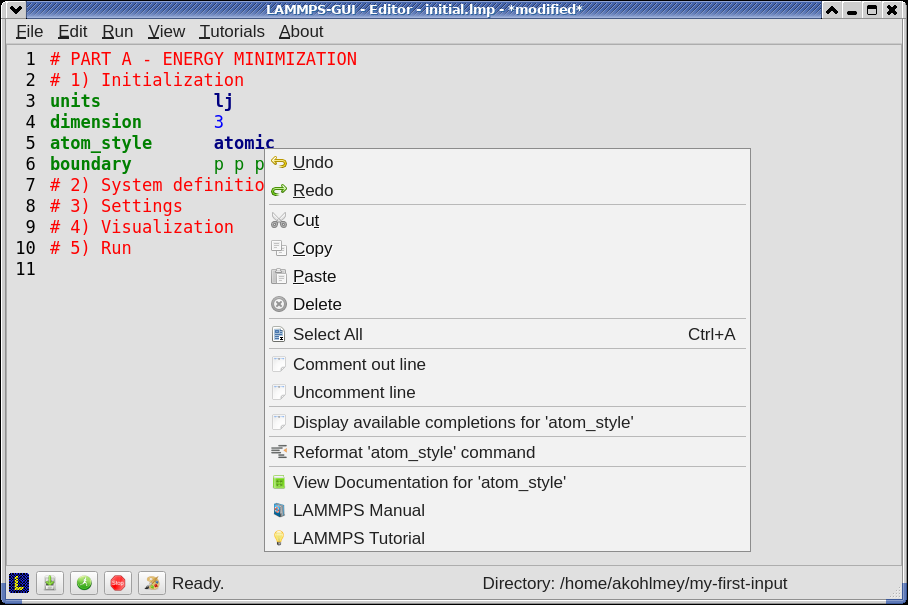
\includegraphics[width=\linewidth]{GUI-1.png}
\caption{A screenshot of the LAMMPS-GUI \guicmd{Editor} window during
  \hyperref[lennard-jones-label]{Tutorial 1}.  The coloring of the text
  is based on the syntax for LAMMPS input files.  The pop-up menu is the
  context menu for right-clicking on the \lmpcmd{atom\_style} line.}
\label{fig:GUI-1}
\end{figure}

Each LAMMPS command is associated with extensive online documentation
detailing the different options for that command.  From the LAMMPS-GUI
editor buffer, the documentation can be accessed by
right-clicking the line with a command, such as \lmpcmd{units lj}, and
selecting \guicmd{View documentation for (\dots)}\,.  LAMMPS--GUI will
prompt your web browser to open the corresponding URL of the online manual.  See
figure~\ref{fig:GUI-1} for a screenshot of this context menu.

\paragraph{System definition}

The next step is to create the simulation box and put some atoms into it.
Modify the \textit{System definition} category of \flecmd{initial.lmp} as follows:
\begin{lstlisting}
# 2) System definition
region simbox block -20 20 -20 20 -20 20
create_box 2 simbox
create_atoms 1 random 1500 34134 simbox overlap 0.3
create_atoms 2 random 100 12756 simbox overlap 0.3
\end{lstlisting}

The first line, \lmpcmd{region simbox (...)}, creates a region
named \lmpcmd{simbox} that is a block (i.e.,~a rectangular
cuboid) extending from -20 to 20 length units along all 3 directions
of space.  % The \lmpcmd{units box} option requests that the region
%dimensions are computed as multiples of the length unit and not as
%multiples of the lattice spacing (\lmpcmd{units lattice}), which is the
%default.  In this specific case there is no difference, since we did not
%use the \lmpcmd{lattice} command and the default lattice spacing is 1.0
%in x-, y-, or z-direction.
% S.G.: I removed "units box", I think it just bring confusion.

The second line, \lmpcmd{create\_box 2 simbox}, creates a simulation box
based on the region \lmpcmd{simbox} with two types of atoms.  From this
point on, any command referencing an atom type larger than \textit{2}
will trigger an error.  You may specify more atom types than
necessary, but for each type you must set the mass and provide
force field parameters.  Failing to do so will cause LAMMPS to abort with an
error at the beginning of a minimization or MD run.

The third line, \lmpcmd{create\_atoms (\dots)}, creates 1500 atoms of type
1 at random positions within the region
\lmpcmd{simbox}.  The integer 34134 is a seed for the
internal random number generator that can be changed to create different
sequences of random numbers and thus different initial geometries for
the simulation.  The fourth line creates 100 atoms of type 2.
Both \lmpcmd{create\_atoms} commands use the optional argument
\lmpcmd{overlap 0.3} to impose a constraint on the randomly placed atoms
so that they must be at least 0.3 length units apart.  This step helps avoid
so-called ``close contacts'' between atoms which can cause
problems due to generating large forces.

\paragraph{Settings}

Next, we specify the settings for the two atom types.  Modify the
\lmpcmd{Settings} category of \flecmd{initial.lmp} as follows:
\begin{lstlisting}
# 3) Settings
mass 1 1.0
mass 2 5.0
pair_style lj/cut 4.0
pair_coeff 1 1 1.0 1.0
pair_coeff 2 2 0.5 3.0
\end{lstlisting}

The two \lmpcmd{mass} commands assign a mass of 1.0 and 5.0 units
to the atoms of type 1 and 2, respectively.  The third line,
\lmpcmd{pair\_style lj/cut 4.0}, specifies that the atoms
will be interacting through a Lennard-Jones (LJ) potential with a
cut-off equal to $r_c = 4.0$ length units
\cite{wang2020lennard,fischer2023history}:
$$E_{ij} (r) = 4 \epsilon_{ij} \left[ \left( \dfrac{\sigma_{ij}}{r} \right)^{12}
  - \left( \dfrac{\sigma_{ij}}{r} \right)^{6} \right], ~ \text{for} ~ r
< r_c,$$ where $r$ is the inter-particle distance, $\epsilon_{ij}$ is
the depth of the potential well, determining the interaction strength, and
$\sigma_{ij}$ is the distance at which the potential energy is zero.
Here, the indexes $ij$ refer to pairs of particle types $i$ and $j$.

The fourth line, \lmpcmd{pair\_coeff 1 1 1.0 1.0}, sets the
Lennard-Jones coefficients for the interactions between pairs of atoms
of type 1, respectively the energy parameter $\epsilon_{11} = 1.0$ and
the distance parameter $\sigma_{11} = 1.0$.  Similarly, the last line
sets the Lennard-Jones coefficients for the interactions between atoms
of type 2, $\epsilon_{22} = 0.5$, and $\sigma_{22} = 3.0$.  By default,
LAMMPS calculates the cross coefficients between the different atom
types using geometric average:
$\epsilon_{ij} = \sqrt{\epsilon_{ii} \epsilon_{jj}}$,
$\sigma_{ij} = \sqrt{\sigma_{ii} \sigma_{jj}}$.  In the present case, we
thus have: $\epsilon_{12} = \sqrt{1.0 \times 0.5} = 0.707$, and
$\sigma_{12} = \sqrt{1.0 \times 3.0} = 1.732$.

\paragraph{Single-point energy}

\begin{figure}
\centering
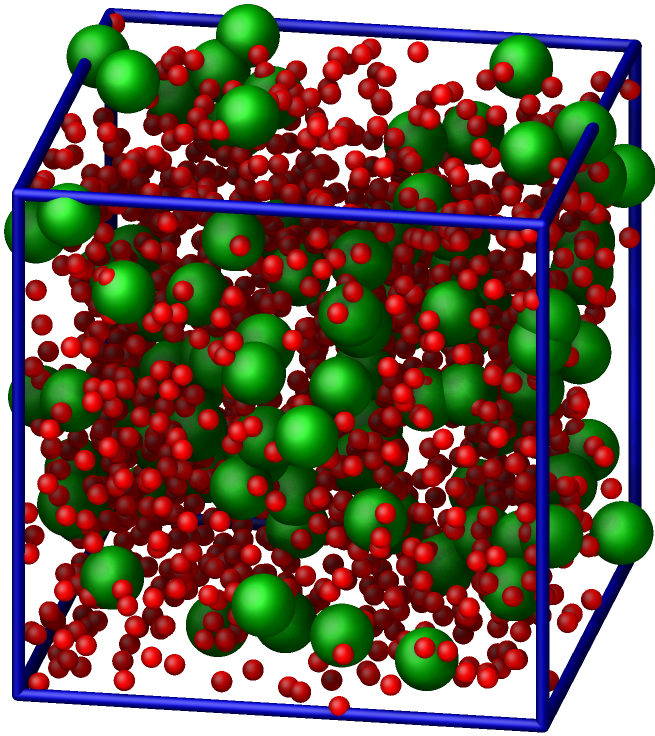
\includegraphics[width=0.55\linewidth]{LJ}
\caption{The binary mixture simulated during \hyperref[lennard-jones-label]{Tutorial 1}.
  The atoms of type 1 are represented as small red spheres, the atoms of type 2 as large
  green spheres, and the edges of the simulation box are represented as blue sticks.}
\label{fig:LJ}
\end{figure}

The system is now fully parameterized, and the input ready to compute
forces.  Let us complete the two remaining categories,
\lmpcmd{Visualization}, and \lmpcmd{Run}, by adding the following lines
into \flecmd{initial.lmp}:
\begin{lstlisting}
# 4) Visualization
thermo 10
thermo_style custom step etotal press
# 5) Run
run 0 post no
\end{lstlisting}

The \lmpcmd{thermo 10} command asks LAMMPS to print thermodynamic
information to the console every given number of steps, in this case,
every 10 simulation steps.  The \lmpcmd{thermo\_style custom} command
specifies what LAMMPS should output -- in this case, the step number
(\textit{step}), total energy (\textit{etotal}), and pressure (\textit{press}).
The \lmpcmd{run 0 post no} command instructs LAMMPS to initialize forces and energy
without actually running the simulation, and the \lmpcmd{post no} option disables
the post-run summary and statistics output.

You can now run LAMMPS.  It should finish quickly, and with the default
settings, LAMMPS--GUI will open two windows: one displaying the console
output and another with a chart.  The \guicmd{Output} window shows information from
the executed commands, along with the total energy and pressure at step 0,
as specified by the thermodynamic data request.  Since no actual simulation
steps were performed, the charts will be empty.

\paragraph{Snapshot Image}

At this point, you can create a snapshot image of the
current system using the \guicmd{Image Viewer} window, which can be
accessed by clicking the \guicmd{Create Image} button in the \guicmd{Run} menu.
The image viewer works by instructing LAMMPS to render an image of the current system using
its internal rendering library via the \lmpcmd{dump image} command.  The
resulting image is then displayed, and various buttons allow you to adjust
the view and rendering style.  The image of
figure~\ref{fig:LJ} was created this way.  This will always capture the current
state of the system.  Save the image for future comparisons.

\paragraph{Energy minimization}

Now, replace the \lmpcmd{run 0 post no} command line with a \lmpcmd{minimize}
command as follows:
\begin{lstlisting}
# 5) Run
minimize 1.0e-6 1.0e-6 1000 10000
\end{lstlisting}

This tells LAMMPS to perform an energy minimization of the system.  That
is, LAMMPS will compute the forces on all atoms and then update the
positions according to a selected algorithm so that the potential energy
decreases.  By default, LAMMPS uses the conjugate gradient (CG)
algorithm \cite{hestenes1952methods}.  The simulation will stop as soon
as the minimizer algorithm cannot find a way to lower the potential
energy.  Except for trivial systems, minimization algorithms will find a
local minimum rather than the global minimum.

Run the minimization and observe that LAMMPS-GUI will capture the output
and update the chart in real time.  This run executes quickly (depending
on your computer's capabilities) and LAMMPS--GUI may fail to capture some
of the thermodynamic data (see figure \ref{fig:chart-log}).  In that
case, use the \guicmd{Preferences} dialog to reduce the data update
interval and switch to single-threaded, unaccelerated execution in the
\guicmd{Accelerators} tab.  You can repeat the run.  Each new run will start
fresh, forgetting the current system and starting over from the top.

\begin{figure}
\centering
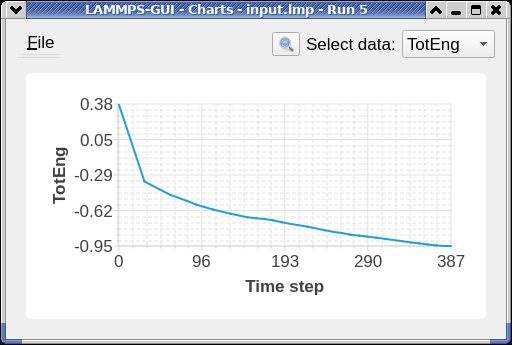
\includegraphics[width=0.49\linewidth]{chart-1}
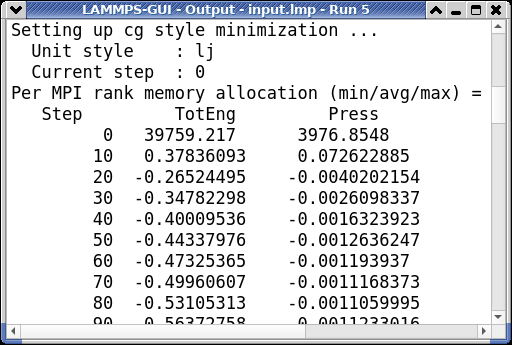
\includegraphics[width=0.497\linewidth]{output-1}
\caption{\guicmd{Charts} (left) and \guicmd{Output} (right) windows of LAMMPS-GUI
  after performing the minimization simulation of \hyperref[lennard-jones-label]{Tutorial 1}.}
\label{fig:chart-log}
\end{figure}

The potential energy decreases from a positive value to a
negative value.  The initially positive value of the potential energy is
expected because the atoms are created at random positions within
the simulation box, with some of them being very close to each other,
resulting in a large initial potential energy due to the repulsive branch of the
Lennard-Jones potential.  As the energy minimization progresses, the
energy decreases -- first rapidly -- then more slowly, and it plateaus at
a negative value, indicating that the atoms are displaced to
reasonable distances from each other.

Create and save a snapshot image of the simulation state after the
minimization and compare the two images.  You should see that the atoms
are ``clumping together''.

Since the \lmpcmd{thermo\_style} command also includes the \textit{press}
keyword, it is possible to switch from plotting the total energy to
displaying the pressure by choosing \guicmd{Press} in the \guicmd{Select data}
drop-down menu of the \guicmd{Charts} window.

\paragraph{Molecular dynamics}

After the energy minimization, any overlapping atoms have been
displaced, and the system is now ready to perform a molecular dynamics
simulation using the minimized geometry.  Since we want to start from
the result of the energy minimization step, we can append commands for
the MD simulation to the same input script, \flecmd{initial.lmp}.  After
the \lmpcmd{minimize} command, add the following lines:
\begin{lstlisting}
# PART B - MOLECULAR DYNAMICS
# 4) Visualization
thermo 50
thermo_style custom step temp etotal pe ke press
\end{lstlisting}

Since LAMMPS reads the input from top to bottom and acts on each line
immediately, these lines will be executed \emph{after} the energy
minimization.  There is no need to re-initialize or re-define the
system.  The \lmpcmd{thermo} command is called a second time to change
the previous value of 10 to a value of 50 as soon as \textit{PART B} of
the simulation starts.  In addition, a new \lmpcmd{thermo\_style}
command changes which thermodynamic information is to be printed by LAMMPS
during \textit{PART B}.  This is done because during molecular
dynamics, the system will have a non-zero temperature (\textit{temp})
and kinetic energy (\textit{ke}) and it is useful to monitor those.
Here, \textit{pe} is the potential energy of the system, such that
\textit{pe + ke = etotal}.

Then, let us add a second \lmpcmd{Run} category by adding the following
lines to \emph{PART B} of \flecmd{initial.lmp}:
\begin{lstlisting}
# 5) Run
fix mynve all nve
timestep 0.005
run 10000
\end{lstlisting}
The \lmpcmd{fix nve} command is used to update the positions and
velocities of the atoms in the group \lmpcmd{all} at every step.  The
group \lmpcmd{all} is a default group that contains every atom.  The
last two lines set the value of the \lmpcmd{timestep} and the number of
steps for the \lmpcmd{run}, respectively, corresponding to a total
duration of 50 time units.

Since there are no other fix commands that change forces or velocities,
and since we have periodic boundary conditions in all directions, the MD
simulation will be performed in the microcanonical or NVE ensemble.
This means the system has no exchange of energy outside the simulation
box and the number of particles and the box volume are constant.  We can
see that there is no equilibrium between potential and kinetic energy
yet, as the former is falling while the latter is rising.  If you extend
the run for more steps (say 100,000), the values for both kinetic and
potential energy will plateau (indicating equilibrium), and the total
energy should fluctuate around some constant value.

Now we change the \lmpcmd{Run} section to:
\begin{lstlisting}
# 5) Run
fix mynve all nve
fix mylgv all langevin 1.0 1.0 0.1 1530917
timestep 0.005
run 10000
\end{lstlisting}

The new command adds a ``Langevin thermostat'' to the atoms in the group
\lmpcmd{all}, with a desired target temperature of 1.0 temperature units
throughout the run (the two numbers stand for the target at the beginning
and at the end of the run, which allows for a temperature ramp if
they differ) \cite{schneider1978molecular}.  A \lmpcmd{damping}
parameter of 0.1 is used.  The \lmpcmd{damping} parameter determines how
rapidly the temperature is relaxed to its desired value.  In a Langevin
thermostat, the atoms are subject to friction and random noise (in the form
of randomly added velocities).  Since a constant friction term removes
more kinetic energy from fast atoms and less from slow atoms, the system
will eventually reach a dynamic equilibrium where the kinetic energy
removed and added are about the same.  The number 1530917 is a
seed used to initialize the random number generator used inside of
\lmpcmd{fix langevin}; you can change it to perform statistically
independent simulations.  In the presence of a thermostat, the MD simulation
will be performed in the canonical or NVT ensemble.

Run the simulation again using LAMMPS. From the information
printed in the \guicmd{Output} window, one can see that the temperature
starts from 0 but rapidly reaches the requested value and
stabilizes itself near $T=1$ temperature units.  One can also see that
the potential energy, $p_\text{e}$, rapidly decreases during energy
minimization (see also figure~\ref{fig:evolution-energy}\,a).  After
the molecular dynamics simulation starts, $p_\text{e}$ increases until
it reaches a plateau value of about -0.25.  The kinetic energy,
$k_\text{e}$, is equal to zero during energy minimization and then
increases during molecular dynamics until it reaches a plateau value of
about 1.5 (Figure~\ref{fig:evolution-energy}\,b).

\begin{figure}
\centering
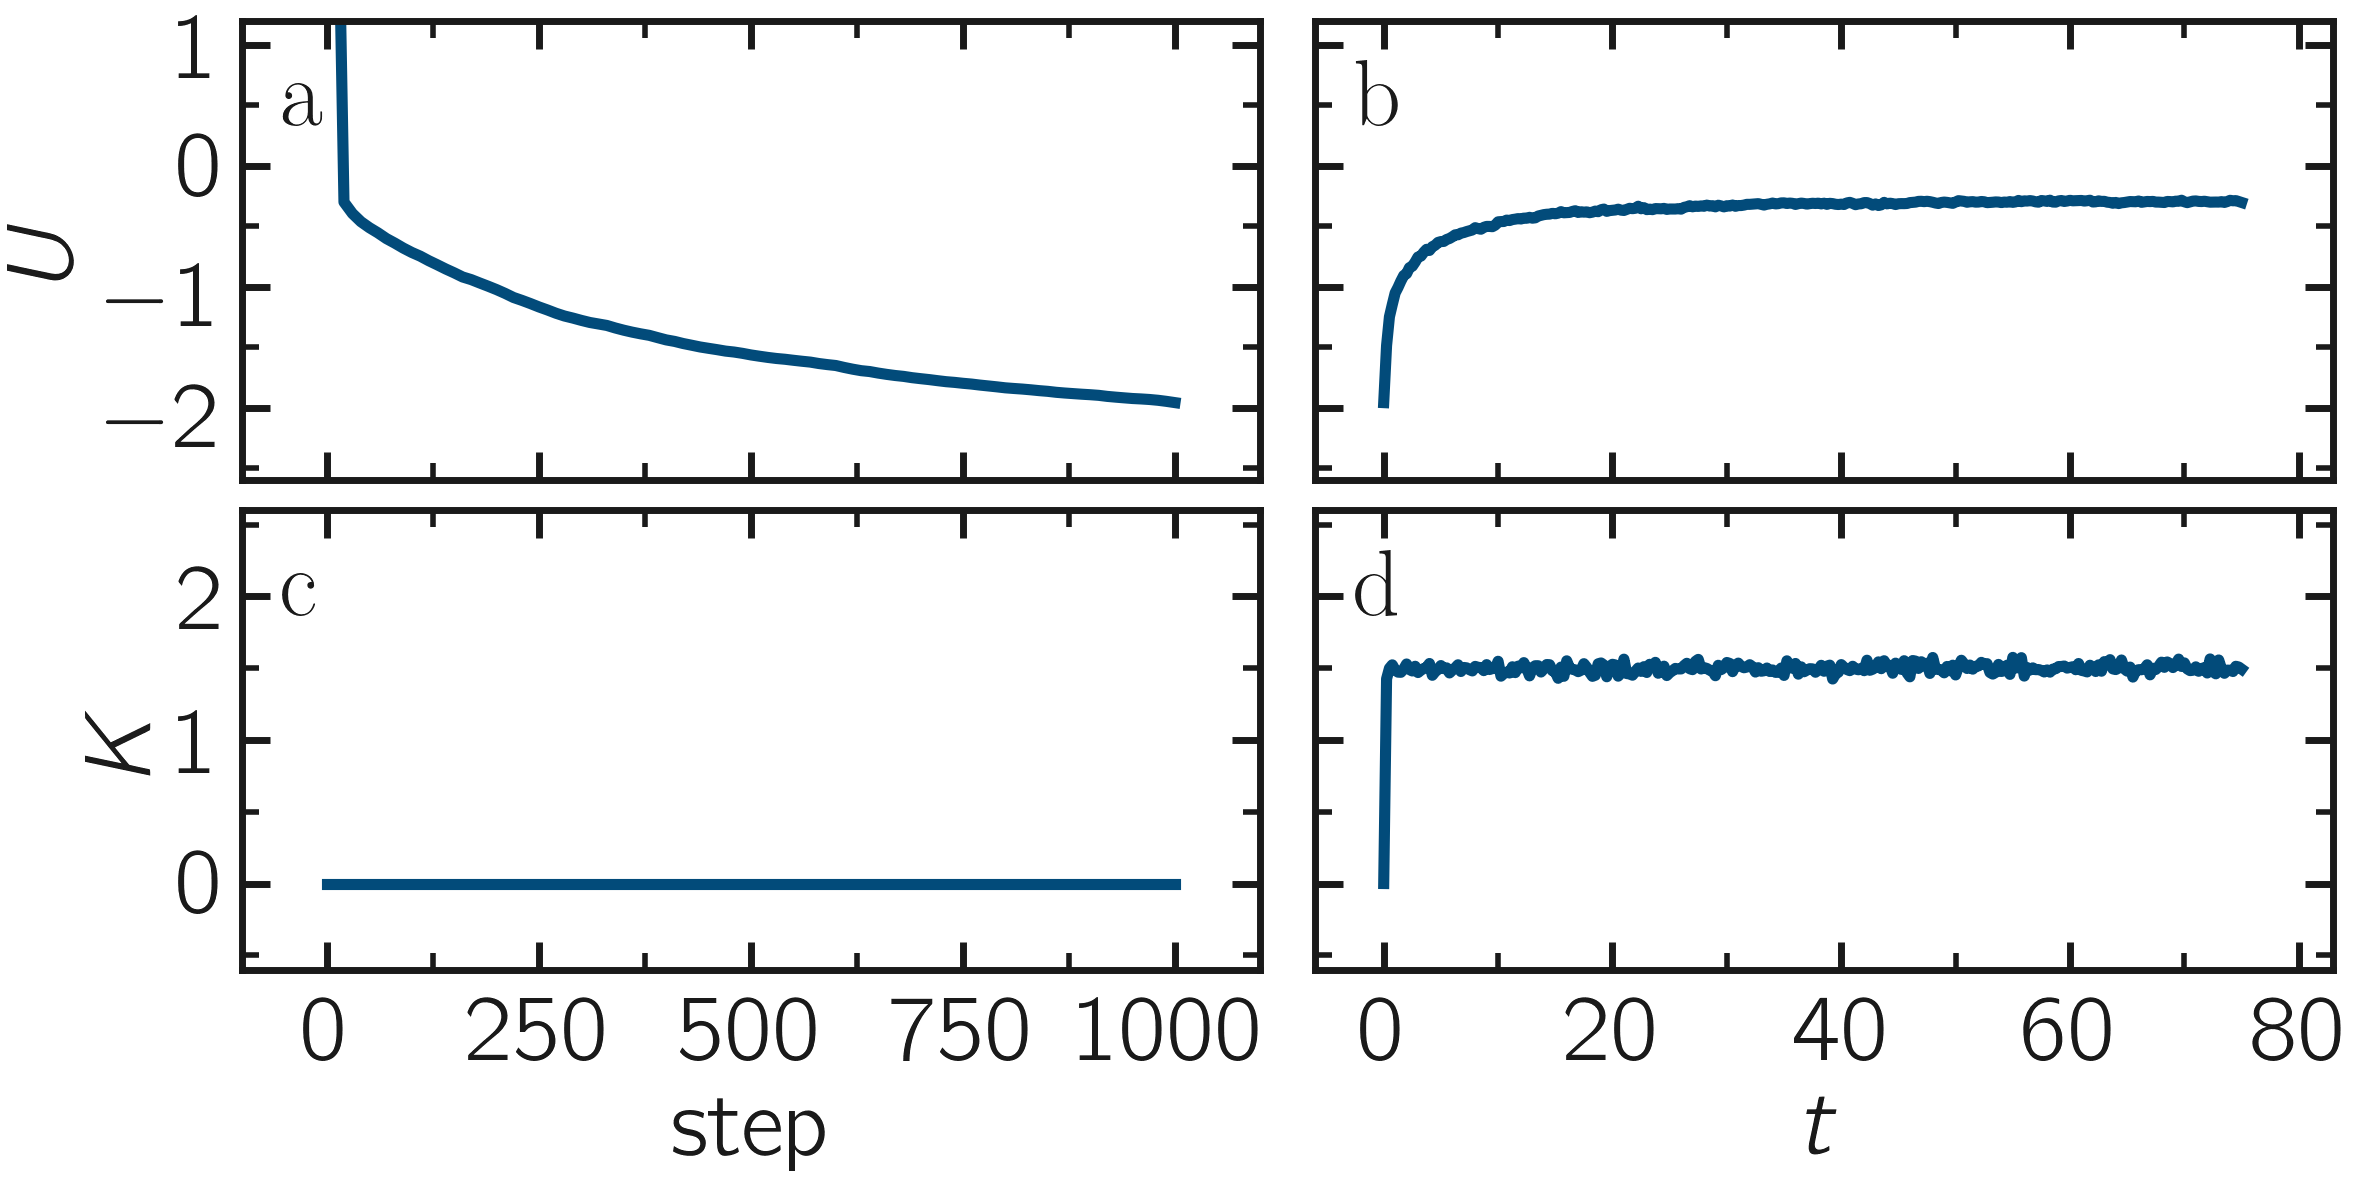
\includegraphics[width=\linewidth]{LJ-energy}
\caption{a)~Potential ($p_\text{e}$) and kinetic energy ($k_\text{e}$) of the
binary mixture simulated during \hyperref[lennard-jones-label]{Tutorial 1} as
functions of the step during energy minimization.
b)~$p_\text{e}$ and $k_\text{e}$ as functions of time $t$ during
molecular dynamics in the NVT ensemble.}
\label{fig:evolution-energy}
\end{figure}

\paragraph{Trajectory visualization}

So far, the simulation has been mostly monitored through the analysis of
thermodynamic information.  To better follow the evolution of the system and visualize
the trajectories of the atoms, let us use the \lmpcmd{dump image} command to
create snapshot images during the simulation.  We have already explored
the \guicmd{Image Viewer} window.  Open it again and adjust the
visualization to your liking using the available buttons.  Now you can
copy the command line used to create this visualization to the clipboard
by either using the \guicmd{Ctrl-D} keyboard shortcut or selecting
\guicmd{Copy dump image command} from the \guicmd{File} menu.  This text
can be pasted into the into the \lmpcmd{Visualization} section of
\lmpcmd{PART B} of the \flecmd{initial.lmp} file.  This may look like the following:

\begin{lstlisting}
dump viz all image 100 myimage-*.ppm type type &
    size 800 800 zoom 1.452 shiny 0.7 fsaa yes &
    view 80 10 box yes 0.025 axes no 0.0 0.0 &
    center s 0.483725 0.510373 0.510373
dump_modify viz pad 9 boxcolor royalblue &
    backcolor white adiam 1 1.6 adiam 2 4.8
\end{lstlisting}
This command tells LAMMPS to generate NetPBM format images every 100
steps.  The two \lmpcmd{type} keywords are for \lmpcmd{color} and
\lmpcmd{diameter}, respectively.  Run the \flecmd{initial.lmp} using
LAMMPS again, and a new window named \guicmd{Slide Show} will pop up.
It will show each image created by the \lmpcmd{dump image} as it is
created and after the simulation is finished (or stopped), the slide
show viewer allows you to animate the trajectory by cycling through the
images.  The window also allows you to export the animation to a movie
(provided the FFMpeg program is installed) and to bulk delete those
image files.

The rendering of the system can be further adjusted using the many
options of the \lmpcmd{dump image} command.  The value for the
\lmpcmd{shiny} keyword is used to adjust the shininess of the atoms, the
\lmpcmd{box} keyword adds or removes a representation of the box, and
the \lmpcmd{view} and \lmpcmd{zoom} keywords adjust the camera (and so
on).

\subsubsection{Improving the script}

Let us improve the input script and perform more advanced operations,
such as specifying initial positions for the atoms and restarting the
simulation from a previously saved configuration.

\paragraph{Control the initial atom positions}

Open the \flecmd{improved.min.lmp}, which was downloaded during the
tutorial setup.  This file contains the \lmpcmd{Part A} of the
\flecmd{initial.lmp} file, but \emph{without} the \lmpcmd{create\_atoms}
commands in the \lmpcmd{System definition} section.

We want to create the atoms of types 1 and 2 in two separate
regions.  To achieve this, we need to add two \lmpcmd{region} commands and then
reintroduce the \lmpcmd{create\_atoms} commands, this time using the new
regions instead of the simulation box region to place the atoms:
\begin{lstlisting}
# 2) System definition
region simbox block -20 20 -20 20 -20 20
create_box 2 simbox
# for creating atoms
region cyl_in cylinder z 0 0 10 INF INF side in
region cyl_out cylinder z 0 0 10 INF INF side out
create_atoms 1 random 1000 34134 cyl_out
create_atoms 2 random 150 12756 cyl_in
\end{lstlisting}
The \lmpcmd{side in} and \lmpcmd{side out} keywords are used to define
regions representing the inside and outside of the cylinder of radius
10 length units.  Then, append a sixth section titled \lmpcmd{Save system} at the end
of the file with the following content (make sure the \lmpcmd{write\_data} command
is placed \emph{after} the \lmpcmd{minimize} command):
\begin{lstlisting}
# 6) Save system
write_data min_coords.data
\end{lstlisting}

A key improvement to the input is the addition of the
\lmpcmd{write\_data} command.  This command writes the state
of the system to a text file called \flecmd{min\_coords.data}.
This \flecmd{.data} file will be used later
to restart the simulation from the final state of the energy
minimization step without having to repeat the system creation and
minimization.

Run the \flecmd{improved.min.lmp} file using LAMMPS.  At the end of the simulation, a file
called \flecmd{min\_coords.data} is created.  You can view the contents
of the file with the file view feature of LAMMPS--GUI, e.g.~from the
\guicmd{File} menu or by right-clicking on the file name in the editor
and selecting the entry \guicmd{View file `min\_coords.data'}.

The created \flecmd{.data} file contains all the information necessary to
restart the simulation, such as the number of atoms, the box size, the
masses, and the pair coefficients.  The
\flecmd{.data} file also contains the final
positions of the atoms within the \lmpcmd{Atoms} section.  The first five
columns of the \lmpcmd{Atoms} section correspond (from left to right) to
the atom indexes (from 1 to the total number of atoms, 1150), the atom
types (1 or 2 here), and the positions of the atoms $x$, $y$, $z$.  The
last three columns are image flags that keep track of which atoms
crossed the periodic boundary.  The exact format of each line in the
\lmpcmd{Atoms} section depends on the choice of \lmpcmd{atom\_style}, which
determines which per-atom data is set and stored internally in LAMMPS.

\begin{note}
  Instead of the \lmpcmd{write\_data} command, you can also use the
  command \lmpcmd{write\_restart improve.min.restart} to save the state
  of the simulation to a binary restart file.  Binary restart files are
  more compact, faster to write, contain more information and thus are
  often more convenient to use.  For example, the choice of atom style
  or pair style is recorded, so those commands do not need to be issued
  before reading the restart.  However, restart files are not expected to be
  portable across LAMMPS versions or platforms.  Thus, in this tutorial,
  we use \lmpcmd{write\_data} so we can provide you with a reference
  copy of the data file in the solutions that will work for you,
  regardless of your LAMMPS version or platform.
\end{note}

\paragraph{Restarting from a saved configuration}

\begin{figure}
\centering
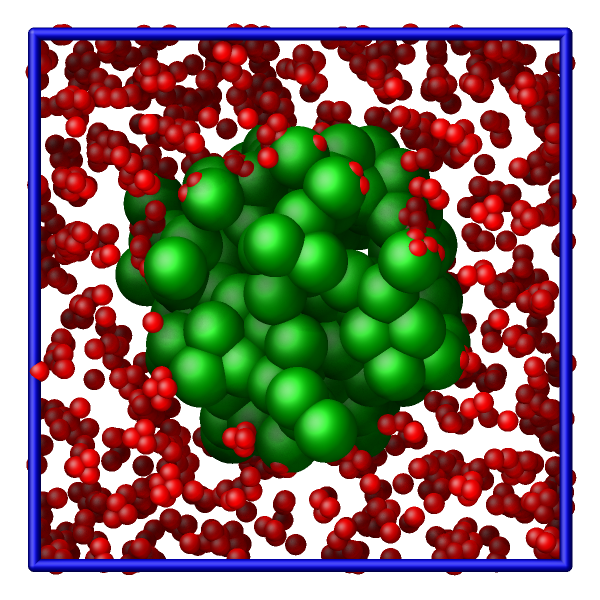
\includegraphics[width=0.55\linewidth]{LJ-cylinder}
\caption{Improved visualization of the binary mixture simulated
during \hyperref[lennard-jones-label]{Tutorial 1}.  The atoms of type 1 are
represented as small red spheres, the atoms of type 2 as large green spheres,
and the edges of the simulation box are represented as blue sticks.}
\label{fig:improved-min}
\end{figure}

To continue a simulation from the saved configuration, open the
\flecmd{improved.md.lmp} file, which was downloaded during the tutorial setup.
This file contains the \textit{Initialization} part from \flecmd{initial.lmp}
and \flecmd{improved.min.lmp}.

Since we want to read the system from the data file, we do not need
to repeat most of the commands from the \lmpcmd{System definition}
and \lmpcmd{Settings} categories.  The exception is the \textit{pair\_style}
command, which now must come \emph{before} the simulation box is defined,
meaning before the \lmpcmd{read\_data} command.  Add the following
lines to \flecmd{improved.md.lmp}:
\begin{lstlisting}
# 2) System definition
pair_style lj/cut 4.0
read_data min_coords.data
\end{lstlisting}

By visualizing the system (see figure \ref{fig:improved-min}), you may
have noticed that some atoms left their original region during
minimization.  To start the simulation from a clean slate, with only
atoms of type 2 inside the cylinder and atoms of type 1 outside the
cylinder, let us delete the misplaced atoms by adding the following
commands to \flecmd{improved.md.lmp}:
\begin{lstlisting}
region cyl_in cylinder z 0 0 10 INF INF side in
region cyl_out cylinder z 0 0 10 INF INF side out
group grp_t1 type 1
group grp_t2 type 2
group grp_in region cyl_in
group grp_out region cyl_out
group grp_t1_in intersect grp_t1 grp_in
group grp_t2_out intersect grp_t2 grp_out
delete_atoms group grp_t1_in
delete_atoms group grp_t2_out
\end{lstlisting}
The first two \lmpcmd{region} commands recreate the previously defined
regions, which is necessary since regions are not saved by the
\lmpcmd{write\_data} command.  The first two \lmpcmd{group} commands
create groups containing all the atoms of type 1 and all the
atoms of type 2, respectively.  The next two \lmpcmd{group} commands
create atom groups based on their positions at the beginning of the
simulation, i.e.~when the commands are being read by LAMMPS.  The last
two \lmpcmd{group} commands create atom groups based on the intersection
between the previously defined groups.  Finally, the two
\lmpcmd{delete\_atoms} commands delete the atoms of type 1
located inside the cylinder and the atoms of type 2 located
outside the cylinder, respectively.

Since LAMMPS has a limited number of custom groups (30), it is good practice
to delete groups that are no longer needed.  This can be done by adding the
following four commands to \flecmd{improved.md.lmp}:
\begin{lstlisting}
# delete unnecessary groups
group grp_in delete
group grp_out delete
group grp_t1_in delete
group grp_t2_out delete
\end{lstlisting}

Let us monitor the number of atoms of each type inside the cylinder as a
function of time by creating the following equal-style variables:
\begin{lstlisting}
variable n1_in equal count(grp_t1,cyl_in)
variable n2_in equal count(grp_t2,cyl_in)
\end{lstlisting}
The equal-style \lmpcmd{variables} are expressions evaluated
during the run and return a number.  Here, they are defined to count
the number of atoms of a specific group within the \lmpcmd{cyl\_in} region.

In addition to counting the atoms in each region, we will also extract
the coordination number of type 2 atoms around type 1 atoms.  The
coordination number measures the number of type 2 atoms near
type 1 atoms, defined by a cutoff distance.  Taking the average provides
as a good indicator of the degree of mixing in a binary mixture.  This
is done using two \lmpcmd{compute} commands:  the first counts the
coordinated atoms, and the second calculates the average over all type 1
atoms.  Add the following lines to \flecmd{improved.md.lmp}:
\begin{lstlisting}
compute coor12 grp_t1 coord/atom cutoff 2 &
  group grp_t2
compute sumcoor12 grp_t1 reduce ave c_coor12
\end{lstlisting}
The \lmpcmd{compute reduce ave} command is used to average the per-atom
coordination number calculated by the \lmpcmd{coord/atom}
compute command.  Compute commands are not automatically invoked; they
require a ``consumer'' command that references the compute.  In this case, the
first compute is referenced by the second, and we reference the second
in a \lmpcmd{thermo\_style custom} command (see below).

\begin{figure}
\centering
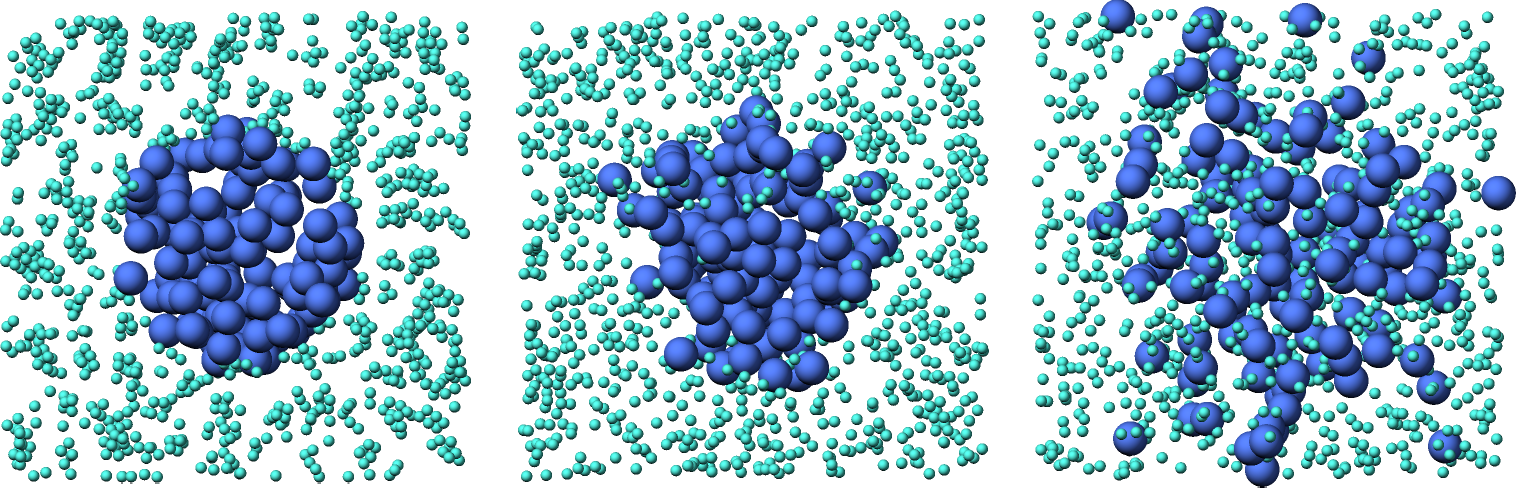
\includegraphics[width=\linewidth]{LJ-evolution}
\caption{Evolution of the system from \hyperref[lennard-jones-label]{Tutorial 1}
during mixing.  The three snapshots show respectively the system
at $t=0$ (left panel), $t=75$ (middle panel), and $t=1500$ (right panel).  The
atoms of type 1 are represented as small turquoise spheres and the atoms of type 2
as large blue spheres.}
\label{fig:evolution-population}
\end{figure}

Finally, let us complete the script by adding the following lines to
\flecmd{improved.md.lmp}.  Note that there is no need for a \lmpcmd{Settings}
section, as the settings are taken from the \flecmd{.data} file.
\begin{lstlisting}
# 4) Visualization
thermo 1000
thermo_style custom step temp pe ke etotal &
  press v_n1_in v_n2_in c_sumcoor12

dump viz all image 100 myimage.md.*.ppm type type &
  shiny 0.1 box no 0.01 view 0 0 zoom 1.8 fsaa yes
dump_modify viz adiam 1 1 adiam 2 3 acolor 1 &
  turquoise acolor 2 royalblue backcolor white
\end{lstlisting}
The two variables \lmpcmd{n1\_in}, \lmpcmd{n2\_in}, along with the compute
\lmpcmd{sumcoor12}, were added to the list of information printed during
the simulation. Additionally, images of the system will be created with
slightly less saturated colors than the default ones. 

Finally, add the following lines to \flecmd{improved.md.lmp}:
\begin{lstlisting}
# 5) Run
velocity all create 1.0 49284 mom yes dist gaussian
fix mynve all nve
fix mylgv all langevin 1.0 1.0 0.1 1530917 zero yes
timestep 0.005
run 300000
\end{lstlisting}

\begin{figure}
\centering
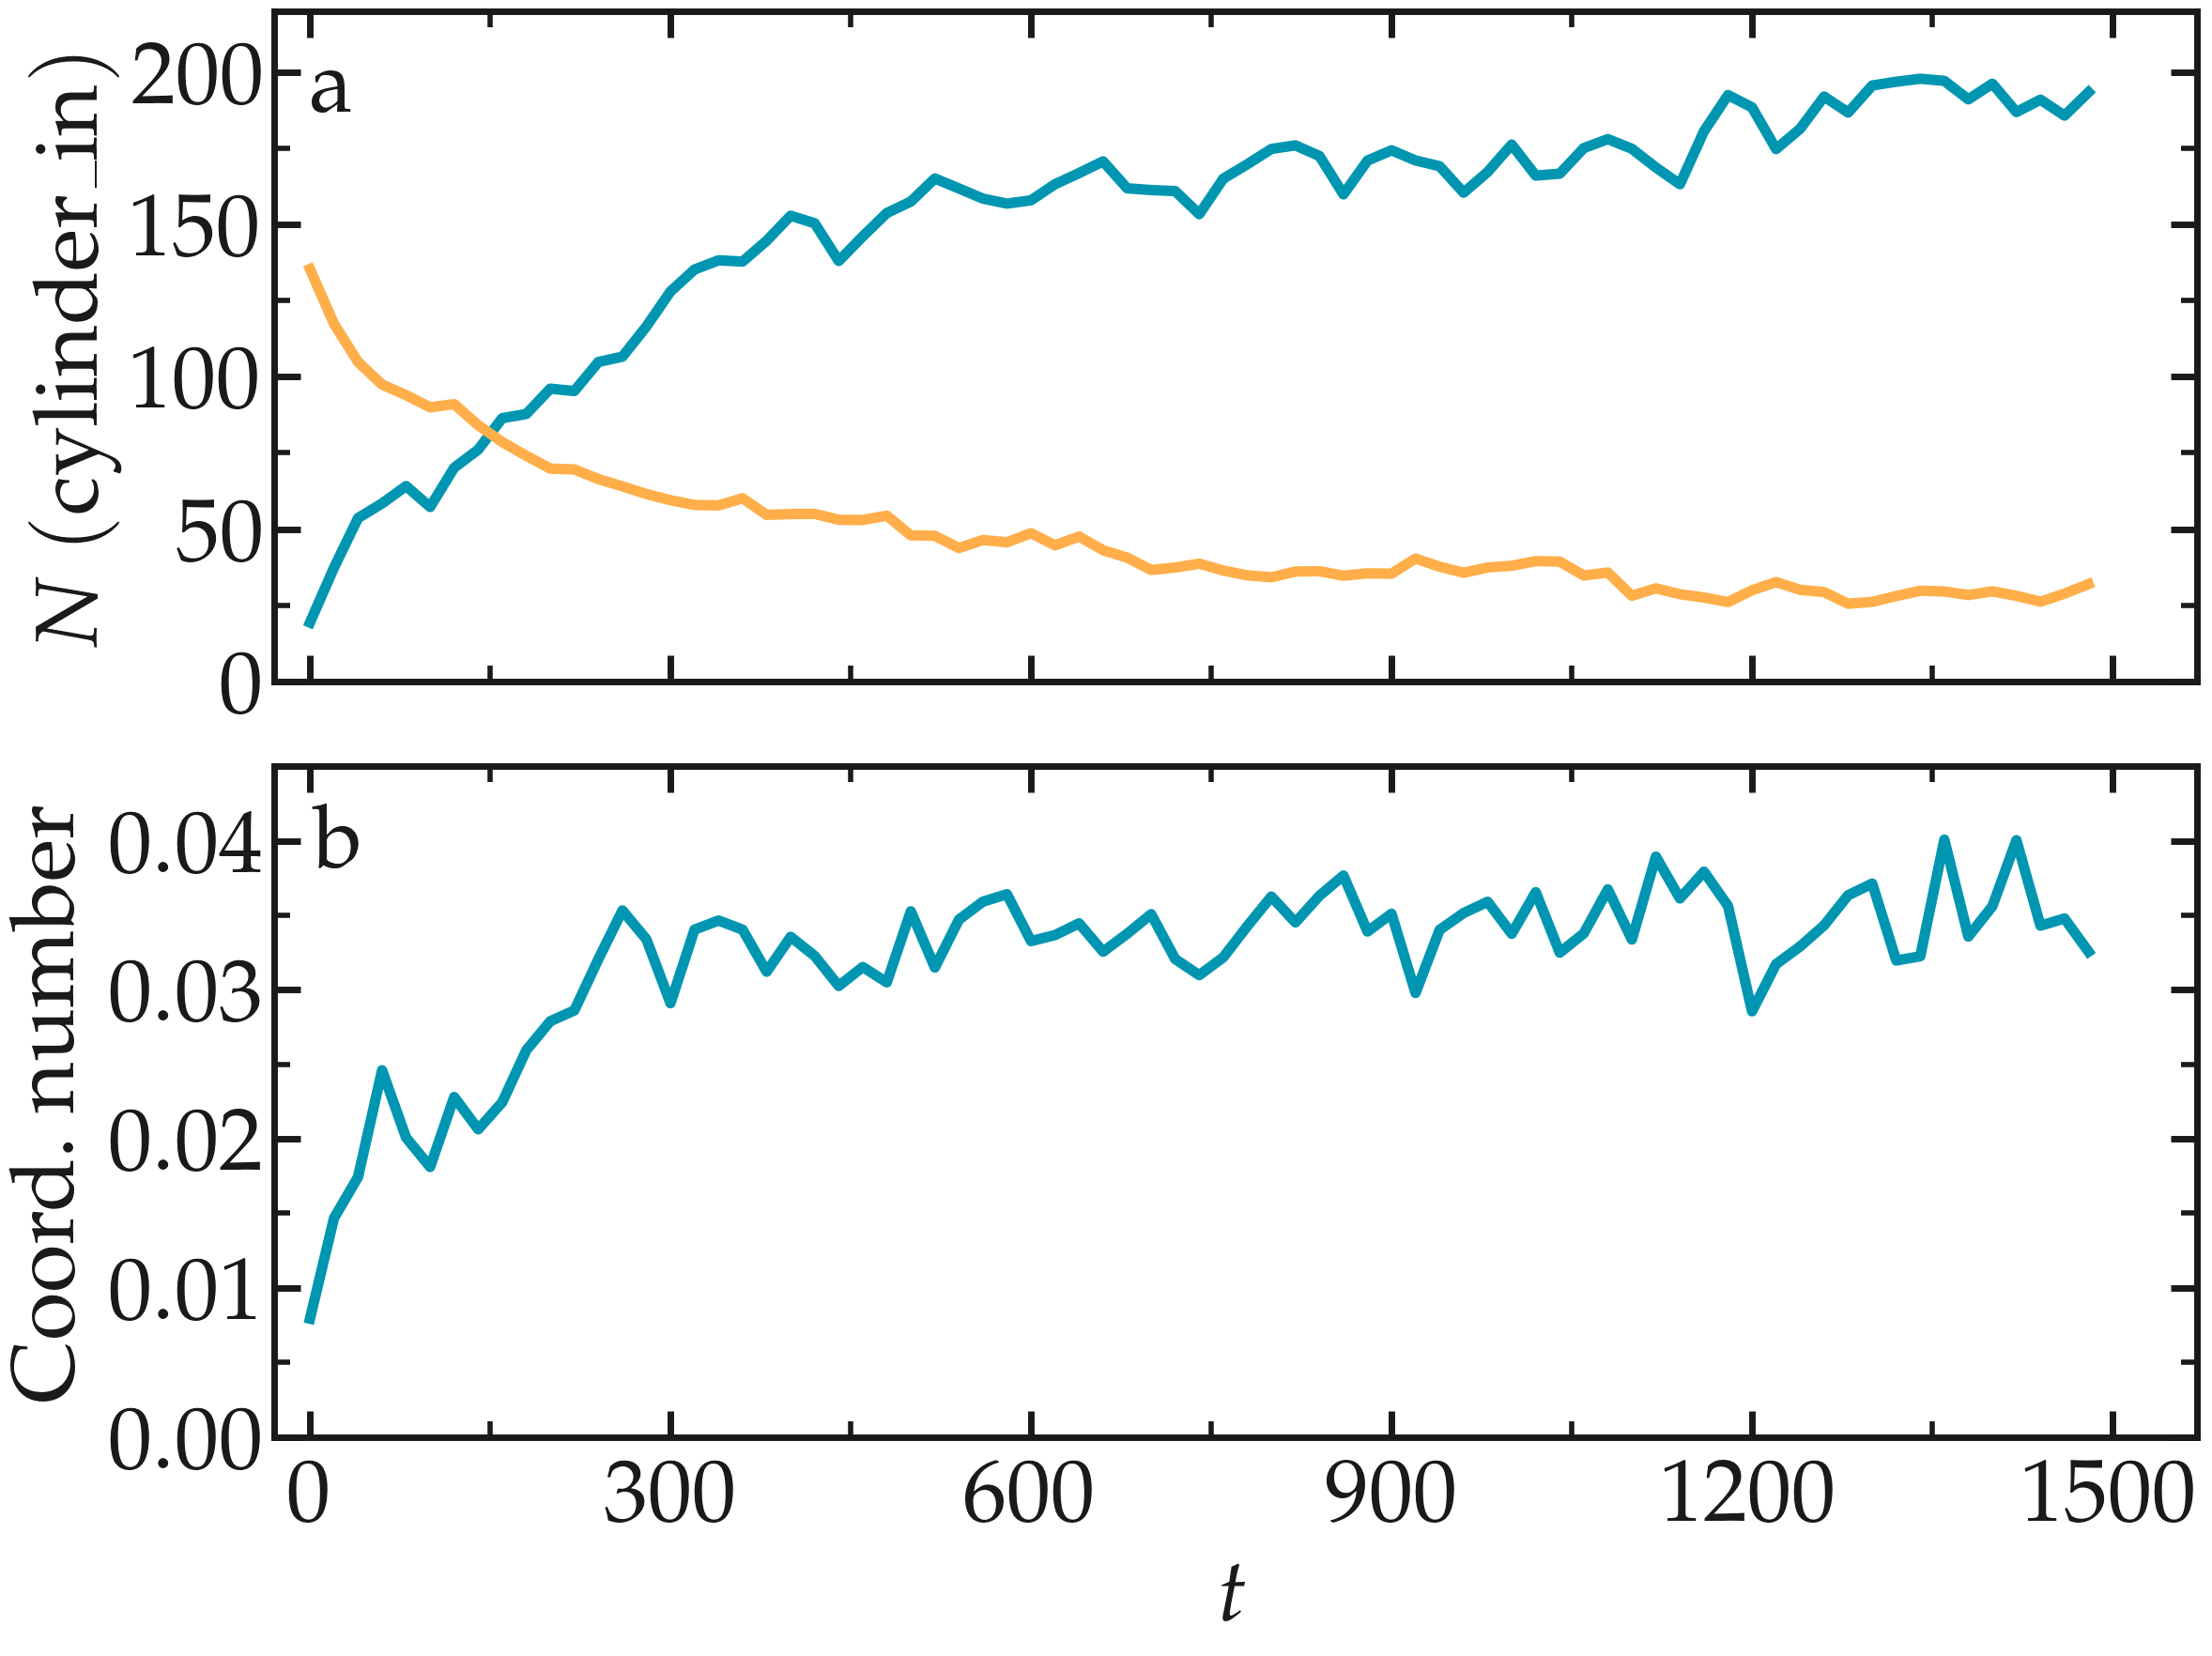
\includegraphics[width=\linewidth]{LJ-mixing}
\caption{a)~Evolution of the numbers $N_\text{1, in}$ and $N_\text{2, in}$ of atoms
of types 1 and 2, respectively, within the \lmpcmd{cyl\_in} region as functions
of time $t$.  b)~Evolution of the coordination number $C_{1-2}$ between atoms of types 1 and 2.}
\label{fig:mixing}
\end{figure}

There are a few more differences from the previous simulation.  First,
the \lmpcmd{velocity create} command assigns an initial velocity to each
atom.  The initial velocity is chosen so that the average initial
temperature is equal to 1.0 temperature units.  The additional keywords
ensure that no linear momentum (\lmpcmd{mom yes}) is given to the
system and that the generated velocities are distributed according to
a Gaussian distribution.  Another improvement is the \lmpcmd{zero yes}
keyword in the Langevin thermostat, which ensures that the total random
force applied to the atoms is equal to zero.

\begin{note}
  The steps to ensure no initial linear momentum and no net random
  force are important to prevent the system from starting to drift or move as a
  whole.  For a bulk system with periodic boundary conditions, it is
  expected to remain in place.  Thus, when computing the temperature from the
  kinetic energy, we use $3N-3$ degrees of freedom since there is no
  global translation.  In a drifting system, some of the kinetic energy is
  due to the drift, which means the system itself cools down.  In
  extreme cases, it can freeze and drift very fast.  This phenomenon is
  sometimes referred to as the ``flying ice cube syndrome'' \cite{wong2016good}.
\end{note}

Run \flecmd{improved.md.lmp} and observe the mixing of the two populations
over time (see also Fig.\,\ref{fig:evolution-population}).  From the
variables \lmpcmd{n1\_in} and \lmpcmd{n2\_in}, you can track the number
of atoms in each region as a function of time
(Fig.\,\ref{fig:mixing}\,a).  To view their evolution, select the entries
\guicmd{v\_n1\_in} or \guicmd{v\_n2\_in} in the \guicmd{Select data} drop-down
menu in the \guicmd{Charts} window of LAMMPS-GUI.

In addition, as the mixing progresses, the average coordination number
between atoms of types 1 and 2 increases from about $0.01$ to $0.04$
(Fig.\,\ref{fig:mixing}\,b).  This indicates that, over time, more and
more particles of type 1 come into contact with particles of type 2, as
expected during mixing.  This can be observed using the entry
\guicmd{c\_sumcoor12} in the \guicmd{Charts} drop-down menu.

\begin{figure}
\centering
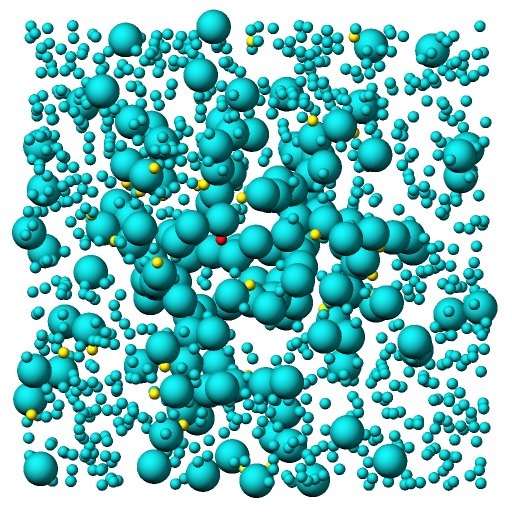
\includegraphics[width=0.55\linewidth]{LJ-coords}
\caption{Snapshot of the binary mixture simulated
  during \hyperref[lennard-jones-label]{Tutorial 1} with atoms of type 1
  colored according to their computed $1-2$ coordination
  number \lmpcmd{c\_coor12}, ranging from turquoise, \lmpcmd{c\_coor12 = 0},
  to yellow, \lmpcmd{c\_coor12 = 1}, and red, \lmpcmd{c\_coor12 = 2}.}
\label{fig:coords-viz}
\end{figure}

\paragraph{Experiments}

Here are some suggestions for further experiments with this system that
may lead to additional insights into how different systems are configured
and how various features function:
\begin{itemize}
\item Use Nos\'e--Hoover thermostat (\lmpcmd{fix nvt}) instead of Langevin
  (\lmpcmd{fix nve} + \lmpcmd{fix langevin}).
\item Omit the energy minimization step for both, Nos\'e--Hoover and Langevin.
\item Apply the thermostat to only one type of atoms and observe the
  temperature for each type separately.
\item Append an NVE run (i.e.~without any thermostat) and observe the energy levels.
\end{itemize}

Another useful experiment to try is to color the atoms in the \guicmd{Slide Show}
according to an observable, such as their respective coordination
numbers.  To do this, replace the
\lmpcmd{dump} and \lmpcmd{dump\_modify} commands with the following lines:
\begin{lstlisting}
variable coor12 atom (type==1)*(c_coor12)+(type==2)*-1
dump viz all image 100 myimage.md.*.ppm v_coor12 &
  type shiny 0.1 box no 0.01 view 0 0 zoom 1.8 fsaa yes
dump_modify viz adiam 1 1 adiam 2 3 backcolor white &
  amap -1 2 ca 0.0 4 min royalblue 0 turquoise 1 yellow max red
\end{lstlisting}
Run LAMMPS again.  Now, the atoms of type 1 are colored based on the value
of \lmpcmd{c\_coor12}, which is mapped continuously from turquoise to yellow
and red for atoms with the highest coordination (Figure~\ref{fig:coords-viz}).
In the definition of the variable \lmpcmd{v\_coor12}, atoms of type 2 are
all assigned a value of -1, and will therefore always be colored their default blue. 

\subsection{Tutorial 2: Pulling on a carbon nanotube}
\label{carbon-nanotube-label}

% "classical" or rather "conventional molecular"?
% SG: "conventional" is indeed better
In this tutorial, the system of interest is a small, single-walled
carbon nanotube (CNT) in an empty box (Fig.\,\ref{fig:CNT}).  The CNT is
strained by fixing atoms at one end and moving atoms at the
other end with constant velocity.  To illustrate the difference between
conventional \cite{typelabel_paper} and reactive force fields, this
tutorial is divided into two parts: in the first part, a conventional molecular force
field (called OPLS-AA \cite{jorgensenDevelopmentTestingOPLS1996}) is
used and the bonds between the atoms of the CNT are unbreakable. In the
second part, a reactive force field (called AIREBO
\cite{stuart2000reactive}) is used, allowing for the breaking of
chemical bonds when the CNT experiences large strain.

To set up this tutorial, select \guicmd{Start Tutorial 2} from the
\guicmd{Tutorials} menu of LAMMPS--GUI and follow the instructions. This will
select a folder, create one if necessary, and place several files into it.
The initial input file, set up for a single-point energy
calculation, will also be loaded into the editor under the name
\flecmd{unbreakable.lmp}.  Additional files are a data file containing the
CNT topology and geometry, named \flecmd{unbreakable.data}, a parameters file
named \flecmd{unbreakable.inc}, as well as the scripts required for the second part
of the tutorial.

\begin{figure}
\centering
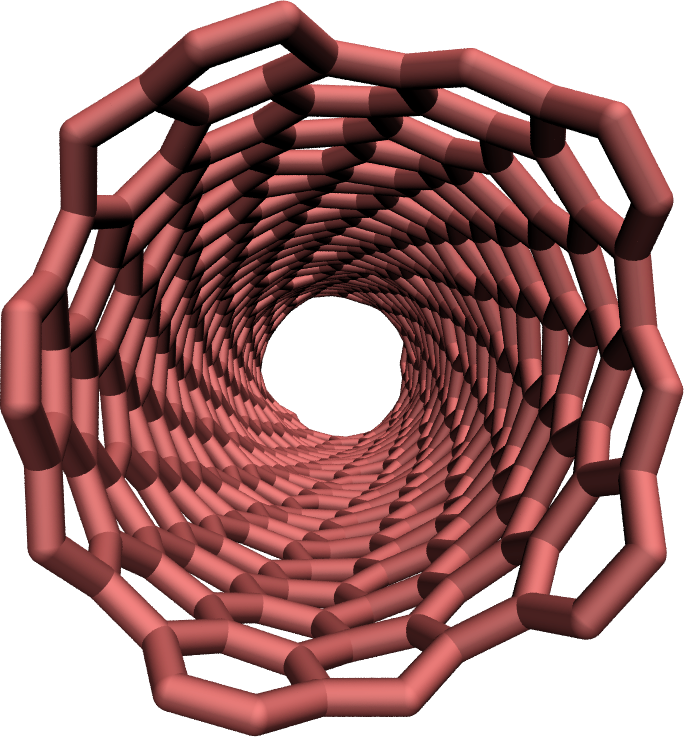
\includegraphics[width=0.55\linewidth]{CNT}
\caption{The carbon nanotube (CNT) simulated during
\hyperref[carbon-nanotube-label]{Tutorial 2}.}
\label{fig:CNT}
\end{figure}

\subsubsection{Unbreakable bonds}

With most conventional molecular force fields, the chemical bonds between
atoms are defined at the start of the simulation and remain fixed, regardless
of the forces applied to the atoms.  These bonds are typically modeled as springs
with equilibrium distances $r_0$ and force constants $k_\text{b}$:
$U_\text{b} = k_\text{b} \left( r - r_0 \right)^2$.  Additionally, angular and
dihedral constraints are often imposed to preserve the molecular structure
by maintaining the relative orientations of neighboring atoms.

\paragraph{The LAMMPS input}

After completing the setup, the editor should display the following content:
\begin{lstlisting}
units real
atom_style molecular
boundary f f f

pair_style lj/cut 14.0
bond_style harmonic
angle_style harmonic
dihedral_style opls
improper_style harmonic
special_bonds lj 0.0 0.0 0.5

read_data unbreakable.data
include unbreakable.inc

run 0 post no
\end{lstlisting}
The chosen unit system is \lmpcmd{real} (therefore distances are in
Ångstrom, times in femtosecond, and energies in kcal/mol), the
\lmpcmd{atom\_style} is \lmpcmd{molecular} (therefore atoms are point particles
that can form bonds with each other), and the boundary conditions are
fixed.  The boundary conditions do not matter here, as the box
boundaries were placed far from the CNT.  Just like in the previous
tutorial, \hyperref[lennard-jones-label]{Lennard-Jones fluid}, the pair
style is \lmpcmd{lj/cut} (i.e.~a Lennard-Jones potential with cutoff)
and its cutoff is set to 14~Ångströms, which means that only the atoms
closer than this distance interact through the Lennard-Jones potential.

The \lmpcmd{bond\_style}, \lmpcmd{angle\_style},
\lmpcmd{dihedral\_style}, and \lmpcmd{improper\_style} commands specify
the different potentials used to constrain the relative positions of the
atoms.  The \lmpcmd{special\_bonds} command sets the weighting factors
for the Lennard-Jones interactions between atoms directly connected by
one bond, two bonds, and three bonds, respectively.  This is done for
convenience when parameterizing the force constants for bonds, angles, and
so on.  By excluding the non-bonded (Lennard-Jones) interactions for
these pairs, those interactions do not need to be considered when determining
the force constants.

The \lmpcmd{read\_data} command imports the
\href{\filepath tutorial2/unbreakable.data}{\dwlcmd{unbreakable.data}}
file, which contains information about the box
size, atom positions, as well as the identity of the atoms that are
linked by \lmpcmd{bonds}, \lmpcmd{angles}, \lmpcmd{dihedrals}, and
\lmpcmd{impropers} interactions.  This file was created using VMD and TopoTools
\cite{kohlmeyer2017topotools}.  The format details of the
different sections in a data file change with different settings.  In
particular, the \lmpcmd{Atoms} section may have a different number of
columns, or the columns may represent different properties when the
\lmpcmd{atom\_style} is changed.  To help users, LAMMPS and tools like
VMD and TopoTools will add a comment (here \lmpcmd{\# molecular}) to the
\lmpcmd{Atoms} header line in the data files that indicates the intended
\lmpcmd{atom\_style}.  LAMMPS will print a warning when the chosen atom
style does not match what is written in that comment.

This data file does not contain any sections with potential parameters; thus,
we need to specify the parameters of both the bonded and
non-bonded potentials.  The parameters we use are taken
from the OPLS-AA (Optimized Potentials for Liquid Simulations-All-Atom)
force field \cite{jorgensenDevelopmentTestingOPLS1996}, and are given
in a separate \lmpcmd{unbreakable.inc} file. This file must be placed within the same
directory as the input file \flecmd{unbreakable.lmp}, and contains the following lines:
\begin{lstlisting}
pair_coeff 1 1 0.066 3.4
bond_coeff 1 469 1.4
angle_coeff 1 63 120
dihedral_coeff 1 0 7.25 0 0
improper_coeff 1 5 180
\end{lstlisting}
% AK: the english here reads a bit "quirky". Jake, any ideas as a native speaker?
The \lmpcmd{pair\_coeff} command sets the parameters for non-bonded
Lennard-Jones interactions atom type 1 to
$\epsilon_{11} = 0.066 \, \text{kcal/mol}$ and
$\sigma_{11} = 3.4 \, \text{\AA{}}$.  The \lmpcmd{bond\_coeff} provides
the equilibrium distance $r_0= 1.4 \, \text{\AA{}}$ and the
spring constant $k_\text{b} = 469 \, \text{kcal/mol/\AA{}}^2$ for the
harmonic potential imposed between two neighboring carbon atoms.  The potential
is given by $U_\text{b} = k_\text{b} ( r - r_0)^2$. The
\lmpcmd{angle\_coeff} gives the equilibrium angle $\theta_0$ and
constant for the potential between three neighboring atoms :
$U_\theta = k_\theta ( \theta - \theta_0)^2$. The
\lmpcmd{dihedral\_coeff} and \lmpcmd{improper\_coeff} define the potentials
for the constraints between 4 atoms.

Rather than copying the contents of the file into the input, we
incorporate it using the \lmpcmd{include} command.  Using \lmpcmd{include} allows
us to conveniently reuse the parameter settings
in other inputs or switch them with others.  This will become more general
when using type labels, which is shown in the next
tutorial \cite{typelabel_paper}.

\paragraph{Prepare the initial state}

In this tutorial, a deformation will be applied to the CNT by displacing
the atoms located at its edges.  To achieve this, we will first isolate the
atoms at the two edges and place them into groups named \lmpcmd{rtop} and
\lmpcmd{rbot}.  Add the following lines to \flecmd{unbreakable.lmp}:
\begin{lstlisting}
group carbon_atoms type 1
variable xmax equal bound(carbon_atoms,xmax)-0.5
variable xmin equal bound(carbon_atoms,xmin)+0.5
region rtop block ${xmax} INF INF INF INF INF
region rbot block INF ${xmin} INF INF INF INF
region rmid block ${xmin} ${xmax} INF INF INF INF
\end{lstlisting}
The first command includes all the atoms of type 1 (i.e.~all the atoms here)
in a group named \lmpcmd{carbon\_atoms}.
The variable $x_\text{max}$ corresponds to the coordinate of the
last atoms along $x$ minus 0.5~Ångströms, and $x_\text{min}$ to the coordinate
of the first atoms along $x$ plus 0.5~Ångströms.  Then, three regions are defined,
corresponding to the following: $x < x_\text{min}$, (\lmpcmd{rbot}, for region
bottom), $x_\text{min} > x > x_\text{max}$ (\lmpcmd{rmid}, for region middle),
and $x > x_\text{max}$ (\lmpcmd{rtop}, for region top).

Finally, let us define 3 groups of atoms corresponding to the atoms
in each of the 3 regions by adding to \flecmd{unbreakable.lmp}:
\begin{lstlisting}
group cnt_top region rtop
group cnt_bot region rbot
group cnt_mid region rmid
set group cnt_top mol 1
set group cnt_bot mol 2
set group cnt_mid mol 3
\end{lstlisting}
With the three \lmpcmd{set} commands, we assign unique, otherwise unused
molecule IDs to atoms in those three groups.  We will use this IDs later to
assign different colors to these groups of atoms.

\begin{figure}
\centering
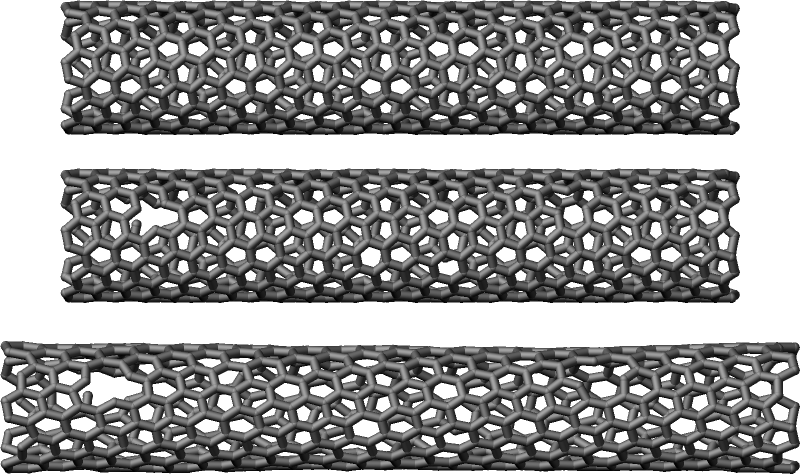
\includegraphics[width=\linewidth]{CNT-unbreakable}
\caption{The unbreakable CNT simulated during \hyperref[carbon-nanotube-label]{Tutorial 2}
before the removal of atoms (top), after the removal of 10 atoms from the \lmpcmd{rmid}
region (middle), and after deformation (bottom).}
\label{fig:CNT-unbreakable}
\end{figure}

Run the simulation using LAMMPS. The number of atoms in each group is given in
the \guicmd{Output} window.  It is an important check to make sure that the number
of atoms in each group corresponds to what is expected, as shown here:
\begin{lstlisting}
10 atoms in group cnt_top
10 atoms in group cnt_bot
680 atoms in group cnt_mid
\end{lstlisting}

Finally, to start from a less ideal state and create a system with some defects,
let us randomly delete a small fraction of the carbon atoms.  To avoid deleting
atoms that are too close to the edges, let us define a new region named \lmpcmd{rdel}
that starts at $2\,\text{\AA{}}$ from the CNT edges:
\begin{lstlisting}
variable xmax_del equal ${xmax}-2
variable xmin_del equal ${xmin}+2
region rdel block ${xmin_del} ${xmax_del} INF INF INF INF
group rdel region rdel
delete_atoms random fraction 0.02 no rdel NULL 2793 bond yes
\end{lstlisting}
The \lmpcmd{delete\_atoms} command randomly deletes $2\,\%$ of the atoms from
the \lmpcmd{rdel} group, here about 10 atoms (compare the top
and the middle panels in Fig.\,\ref{fig:CNT-unbreakable}).

\paragraph{The molecular dynamics}

Let us give an initial temperature to the atoms of the group \lmpcmd{cnt\_mid}:
\begin{lstlisting}
reset_atoms id sort yes
velocity cnt_mid create 300 48455 mom yes rot yes
\end{lstlisting}
Re-setting the atom IDs is necessary before using the \lmpcmd{velocity} command
when atoms were deleted, which is done here with the \lmpcmd{reset\_atoms} command.
The \lmpcmd{velocity} command gives initial velocities to the atoms of the middle
group \lmpcmd{cnt\_mid}, ensuring an initial temperature of $T = 300\,\text{K}$
for these atoms.

Let us specify the thermalization and the dynamics of the system. Add the following
lines into \flecmd{unbreakable.lmp}:
\begin{lstlisting}
fix mynve1 cnt_top nve
fix mynve2 cnt_bot nve
fix mynvt cnt_mid nvt temp 300 300 100
\end{lstlisting}
The \lmpcmd{fix nve} are applied to the atoms of \lmpcmd{cnt\_top} and
\lmpcmd{cnt\_bot}, respectively, and will ensure that the positions of the atoms
from these groups are recalculated at every step.  The \lmpcmd{fix nvt} does the
same for the \lmpcmd{cnt\_mid} group, while also applying a Nos\'e-Hoover thermostat
with desired temperature of 300\,K \cite{nose1984unified, hoover1985canonical}.
To restrain the motion of the atoms at the edges, let us add the following
commands to \flecmd{unbreakable.lmp}:
\begin{lstlisting}
fix mysf1 cnt_top setforce 0 0 0
fix mysf2 cnt_bot setforce 0 0 0
velocity cnt_top set 0 0 0
velocity cnt_bot set 0 0 0
\end{lstlisting}
The two \lmpcmd{setforce} commands cancel the forces applied on the atoms of the
two edges, respectively.  The cancellation of the forces is done at every step,
and along all 3 directions of space, $x$, $y$, and $z$, due to the use of
\lmpcmd{0 0 0}.  The two \lmpcmd{velocity} commands set the initial velocities
along $x$, $y$, and $z$ to 0 for the atoms of \lmpcmd{cnt\_top} and
\lmpcmd{cnt\_bot}, respectively.  As a consequence of these last four commands,
the atoms of the edges will remain immobile during the simulation (or at least
they would if no other command was applied to them).

\begin{note}
  The \lmpcmd{velocity set}
  commands impose the velocity of a group of atoms at the start of a run but do
  not enforce the velocity during the entire simulation. When \lmpcmd{velocity set}
  is used in combination with \lmpcmd{setforce 0 0 0}, as is the case here, the
  atoms won't feel any force during the entire simulation.  According to the Newton
  equation, no force means no acceleration, meaning that the initial velocity
  will persist during the entire simulation, thus producing a constant velocity motion.
\end{note}

\paragraph{Outputs}
Next, to measure the strain and stress applied to the CNT, let us create a
variable for the distance $L_\text{cnt}$ between the two edges,
as well as a variable $F_\text{cnt}$ for the force applied on the edges:
\begin{lstlisting}
variable Lcnt equal xcm(cnt_top,x)-xcm(cnt_bot,x)
variable Fcnt equal f_mysf1[1]-f_mysf2[1]
\end{lstlisting}
Here, the force is extracted from the fixes \lmpcmd{mysf1} and \lmpcmd{mysf2}
using \lmpcmd{f\_}, similarly to the use of \lmpcmd{v\_} to call a variable,
and \lmpcmd{c\_} to call a compute, as seen in \hyperref[lennard-jones-label]{Tutorial 1}.

Let us also add a \lmpcmd{dump image} command to visualize the system
every 500 steps:
\begin{lstlisting}
dump viz all image 500 myimage-*.ppm element type size &
  1000 400 zoom 6 shiny 0.3 fsaa yes bond atom 0.8 &
  view 0 90 box no 0.0 axes no 0.0 0.0
dump_modify viz pad 9 backcolor white adiam 1 0.85 bdiam 1 1.0
\end{lstlisting}
Let us run a small equilibration step to bring the system to the required
temperature before applying any deformation:
\begin{lstlisting}
compute Tmid cnt_mid temp
thermo 100
thermo_style custom step temp etotal v_Lcnt v_Fcnt
thermo_modify temp Tmid line yaml

timestep 1.0
run 5000
\end{lstlisting}
With the \lmpcmd{thermo\_modify} command, we specify to LAMMPS that the
temperature $T_\mathrm{mid}$ of the middle group, \lmpcmd{cnt\_mid},
must be outputted, instead of the temperature of the entire system.
This choice is motivated by the presence of
frozen parts with an effective temperature of 0\,K, which makes the average
temperature of the entire system less relevant.  The \lmpcmd{thermo\_modify}
command also imposes the use of the YAML format that can easily be read by
Python (see below).

Let us impose a constant velocity deformation on the CNT
by combining the \textit{velocity set} command with previously defined
\lmpcmd{fix setforce}.  Add the following lines in the \lmpcmd{unbreakable.lmp}
file, right after the last \lmpcmd{run 5000} command:
\begin{lstlisting}
velocity cnt_top set 0.0005 0 0
velocity cnt_bot set -0.0005 0 0

run 10000
\end{lstlisting}
The chosen velocity for the deformation is $100\,\text{m/s}$, or
$0.001\,\text{\AA{}/fs}$.

\begin{figure}
\centering
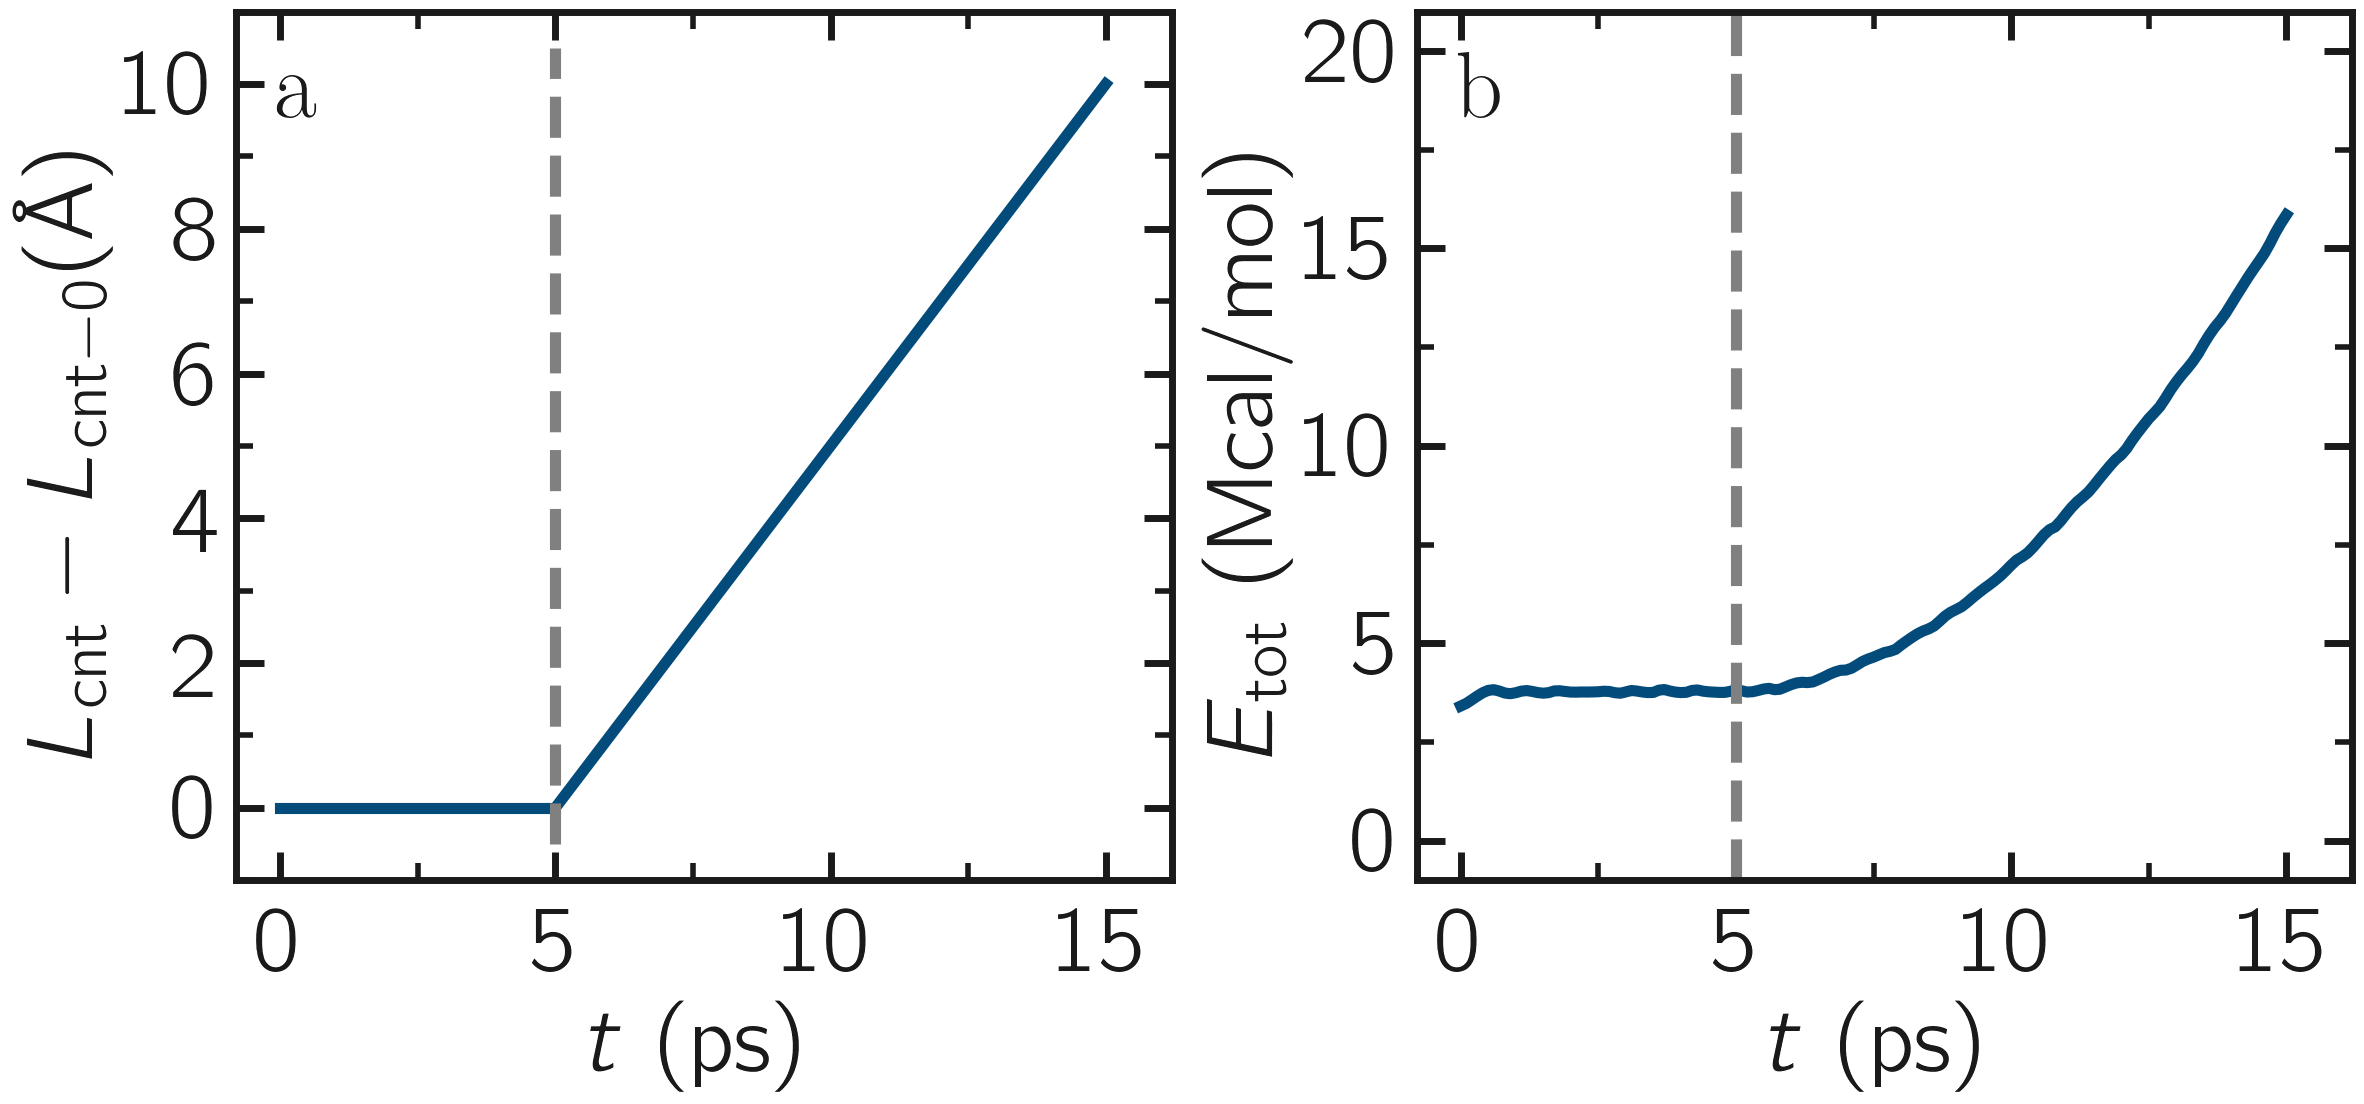
\includegraphics[width=\linewidth]{CNT-unbreakable-length-energy}
\caption{a) Evolution of the length $L_\text{cnt}$ of the CNT with time,
as simulated during \hyperref[carbon-nanotube-label]{Tutorial 2}.
The CNT starts deforming at $t = 5\,\text{ps}$, and $L_\text{cnt-0}$ is the
CNT initial length. b) Evolution of the total energy $E_\text{tot}$ of the system
with time $t$. Here, the potential is OPLS-AA, and the CNT is unbreakable.}
\label{fig:CNT-unbreakable-LE}
\end{figure}

Run the simulation using LAMMPS.  As can be seen from the variable $L_\text{cnt}$, the length
of the CNT increases linearly over time for $t > 5\,\text{ps}$ (Fig.\,\ref{fig:CNT-unbreakable-LE}\,a),
as expected from the imposed constant velocity.  What you observe in the \guicmd{Slide Show}
windows should resembles Fig.\,\ref{fig:CNT-unbreakable}.  The total energy of the system
shows a non-linear increase with $t$ once the deformation starts, which is expected
from the typical dependency of bond energy with bond distance,
$U_\text{b} = k_\text{b} \left( r - r_0 \right)^2$ (Fig.\,\ref{fig:CNT-unbreakable-LE}\,b).

\paragraph{Importing YAML log file into Python}

Let us import the simulation data into Python, and generate a stress-strain curve.
Here, the stress is defined as $F_\text{cnt}/A_\text{cnt}$,
where $A_\text{cnt} = \pi r_\text{cnt}^2$ is the surface area of the
CNT, and $r_\text{cnt}=5.2$\,\AA{} the CNT radius.  The strain is defined
as $(L_\text{cnt}-L_\text{cnt-0})/L_\text{cnt-0}$, where $L_\text{cnt-0}$ is the initial CNT length.

Right-click inside the \guicmd{Output} window, and select
\guicmd{Export YAML data to file}.  Call the output \flecmd{unbreakable.yaml}, and save
it within the same folder as the input files, where a Python script named
\href{\filepath tutorial2/yaml-reader.py}{\dwlcmd{yaml-reader.py}} should also
be located.  When executed using Python, this .py file first imports
the \flecmd{unbreakable.yaml} file.  Then, a certain pattern is
identified and stored as a string character named `docs'.  The string is
then converted into a list, and $F_\text{cnt}$ and $L_\text{cnt}$
are extracted.  The stress and strain
are then calculated, and the result is saved in a data file using the
NumPy `savetxt' function.  `thermo[0]' can be used to access the
information from the first minimization run, and `thermo[1]' to access the
information from the second MD run.  The data extracted from
the \flecmd{unbreakable.yaml} file can then be used to plot the stress-strain
curve, see Fig.\,\ref{fig:CNT-stress-strain-unbreakable}.

\begin{figure}
\centering
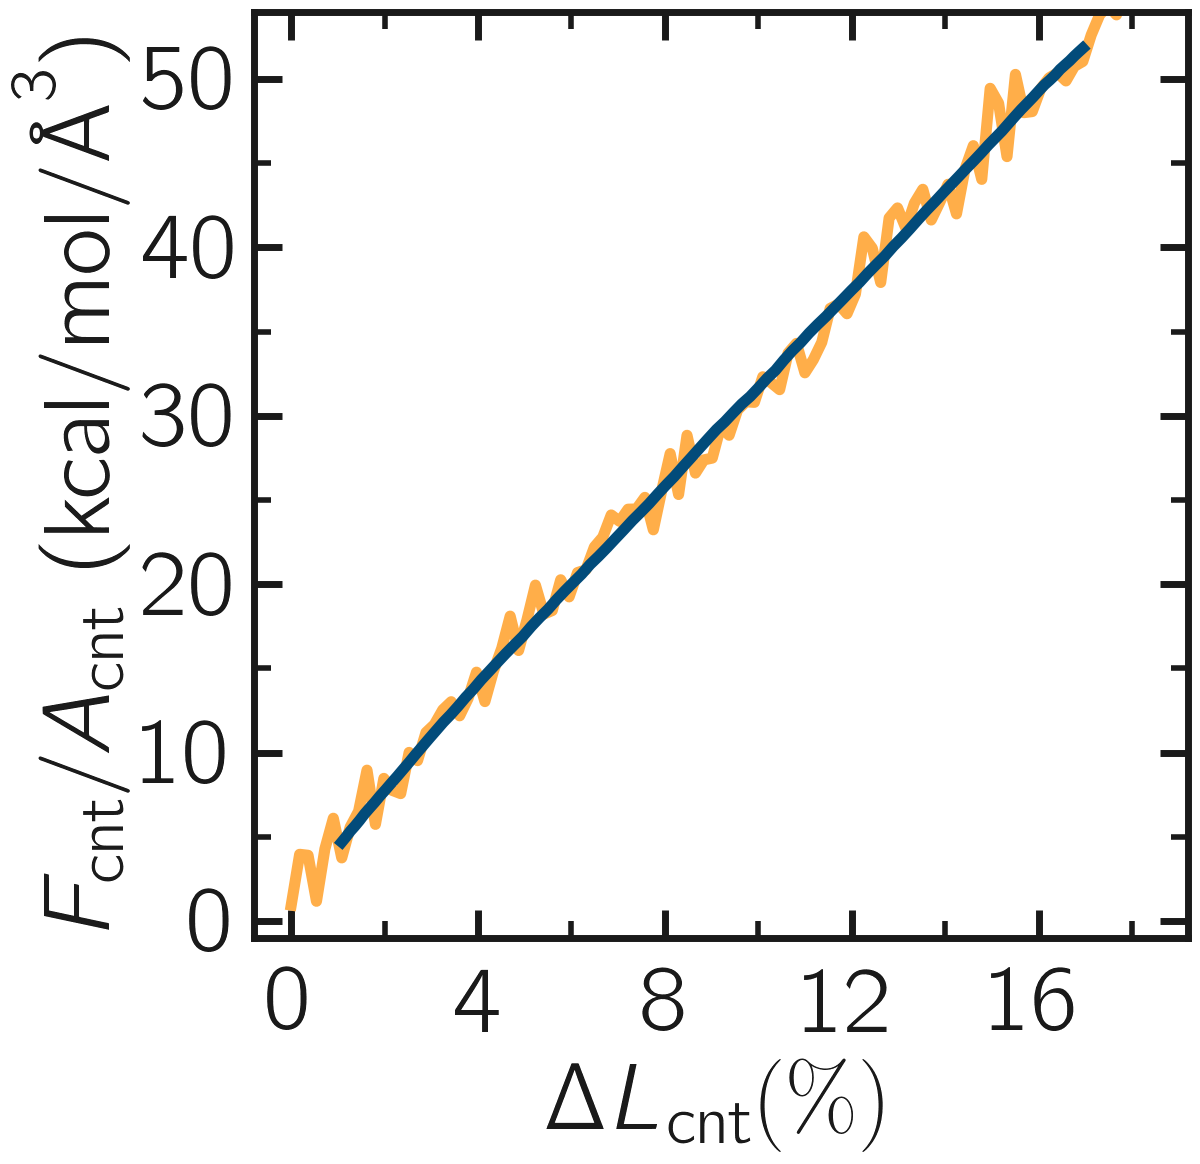
\includegraphics[width=0.55\linewidth]{CNT-unbreakable-stress-strain}
\caption{Stress applied on the CNT during deformation, $F_\text{cnt}/A_\text{cnt}$,
where $F_\text{cnt}$ is the force and $A_\text{cnt}$ the CNT surface area,
as a function of the strain, $\Delta L_\text{cnt} = (L_\text{cnt}-L_\text{cnt-0}/L_\text{cnt-0})$, where
$L_\text{cnt}$ is the CNT length and $L_\text{cnt-0}$ the CNT initial length,
as simulated during \hyperref[carbon-nanotube-label]{Tutorial 2}.
Here, the potential is OPLS-AA, and the CNT is unbreakable.}
\label{fig:CNT-stress-strain-unbreakable}
\end{figure}

\subsubsection{Breakable bonds}

When using a conventional molecular force field, as we have just done, the bonds between the atoms
are non-breakable.  Let us perform a similar simulation and deform a small
CNT again, but this time with a reactive force field that allows bonds
to break if the applied deformation is large enough.

\paragraph{Input file initialization}

Open the input named 
\href{\filepath tutorial2/breakable.lmp}{\dwlcmd{breakable.lmp}} that should have
been downloaded next to \lmpcmd{unbreakable.lmp} during the tutorial setup.
There are only a few differences with the previous input.  First, the \lmpcmd{metal}
units system is used instead of \lmpcmd{real}, which is
required by the AIREBO force field.  A second difference is the use of the
\lmpcmd{atom\_style atomic} instead of \lmpcmd{molecular}, since no explicit
bond information is required with AIREBO. The following commands are
setting up the AIREBO force field:
\begin{lstlisting}
pair_style airebo 3.0
pair_coeff * * CH.airebo C
\end{lstlisting}
Here, \href{\filepath tutorial2/CH.airebo}{\dwlcmd{CH.airebo}} is the file
containing the parameters for AIREBO, and must be placed next
to \lmpcmd{breakable.lmp}.

\begin{note}
  With the \lmpcmd{metal} units system, times are in picoseconds ($10^{-12}$\,s)
  instead of femtoseconds ($10^{-15}$\,s) in the case of the \lmpcmd{real} units system.
  It is important to keep this in mind when setting parameters that are expressed
  in time unit, such as the timestep or the time constant of the thermostat.
\end{note}

\paragraph{Adapt the topology file}

Since bonds, angles, and dihedrals do not need to be
explicitly set when using AIREBO, some simplification must be made to the
\flecmd{.data} file.  The new \flecmd{.data}
file is named \href{\filepath tutorial2/breakable.data}{\dwlcmd{breakable.data}},
and must be placed within the same folder as the input file.  Just like \flecmd{unbreakable.data},
the \flecmd{breakable.data} contains the information
required for placing the atoms in the box, but no bond/angle/dihedral information.
Another difference between the \flecmd{unbreakable.data} and \flecmd{breakable.data} files
is that, here, a larger distance of 120~Ångströms was used for the box size along
the $x$ axis, to allow for larger deformation of the CNT.

\paragraph{Start the simulation}

Here, let us perform a similar deformation as the previous one. 
In \lmpcmd{breakable.lmp}, replace the \lmpcmd{run 0 post no} line with:
\begin{lstlisting}
fix mysf1 cnt_bot setforce 0 0 0
fix mysf2 cnt_top setforce 0 0 0
velocity cnt_bot set 0 0 0
velocity cnt_top set 0 0 0

variable Lcnt equal xcm(cnt_top,x)-xcm(cnt_bot,x)
variable Fcnt equal f_mysf1[1]-f_mysf2[1]

dump viz all image 500 myimage.*.ppm type type size 1000 400 &
  zoom 4 shiny 0.3 adiam 1.5 box no 0.01 view 0 90 &
  shiny 0.1 fsaa yes
dump_modify viz pad 5 backcolor white acolor 1 gray

compute Tmid cnt_mid temp
thermo 100
thermo_style custom step temp etotal v_Lcnt v_Fcnt
thermo_modify temp Tmid line yaml

timestep 0.0005
run 10000
\end{lstlisting}
Note the relatively small timestep of $0.0005$\,ps ($= 0.5$\,fs) used. Reactive force
fields like AIREBO usually require a smaller timestep than conventional ones.  When running
\flecmd{breakable.lmp} with LAMMPS, you can see that the temperature deviates
from the target temperature of $300\,\text{K}$ at the start of the equilibration,
but that after a few steps, it reaches the target value.

\begin{note}
  Bonds cannot be displayed by the \lmpcmd{dump image} when using
  the \lmpcmd{atom\_style atomic}, as it contains no bonds. A tip for displaying bonds
  with the present system is provided at the end of the tutorial.
\end{note}

\paragraph{Launch the deformation}

After equilibration, let us set the velocity of the edges equal to
$75~\text{m/s}$ (or $0.75~\text{\AA{}/fs}$) and run for a longer duration than
previously. Add the following lines into \flecmd{breakable.lmp}:
\begin{lstlisting}
velocity cnt_top set 0.75 0 0
velocity cnt_bot set -0.75 0 0

run 30000
\end{lstlisting}
Run the simulation.  Some bonds are expected to break before the end of the
simulation (Fig.\,\ref{fig:CNT-deformed-breakable}).

\begin{figure}
\centering
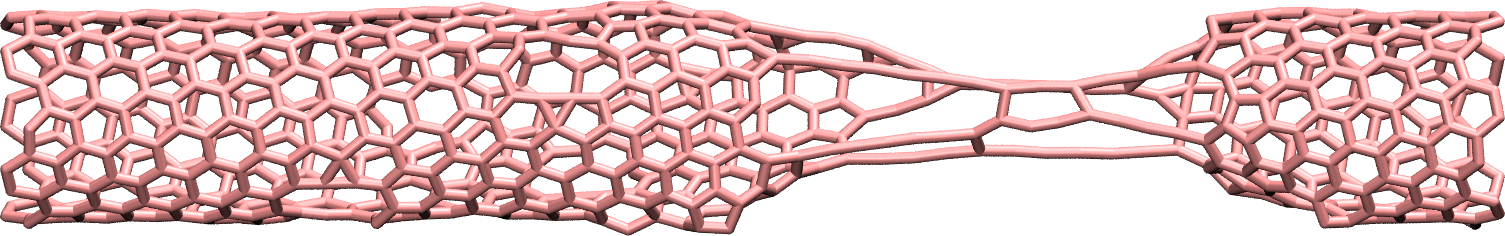
\includegraphics[width=\linewidth]{CNT-deformed-breakable}
\caption{CNT with broken bonds. This image was geenrated using
VMD \cite{vmd_home,humphrey1996vmd} with the \guicmd{DynamicBonds} representation.}
\label{fig:CNT-deformed-breakable}
\end{figure}

Looking at the evolution of the energy, one can see that the total energy $E_\text{tot}$ is initially increasing with the deformation. When bonds break, the energy relaxes abruptly,
as can be seen near $t=110~\text{ps}$ and again near $t=130~\text{ps}$ in
Fig.\,\ref{fig:CNT-deformed-breakable}\,a. Using the same script as previously to
import the data into Python, the stress-strain
curve can be generated, see Fig.\,\ref{fig:CNT-deformed-breakable}\,b.

\begin{figure}
\centering
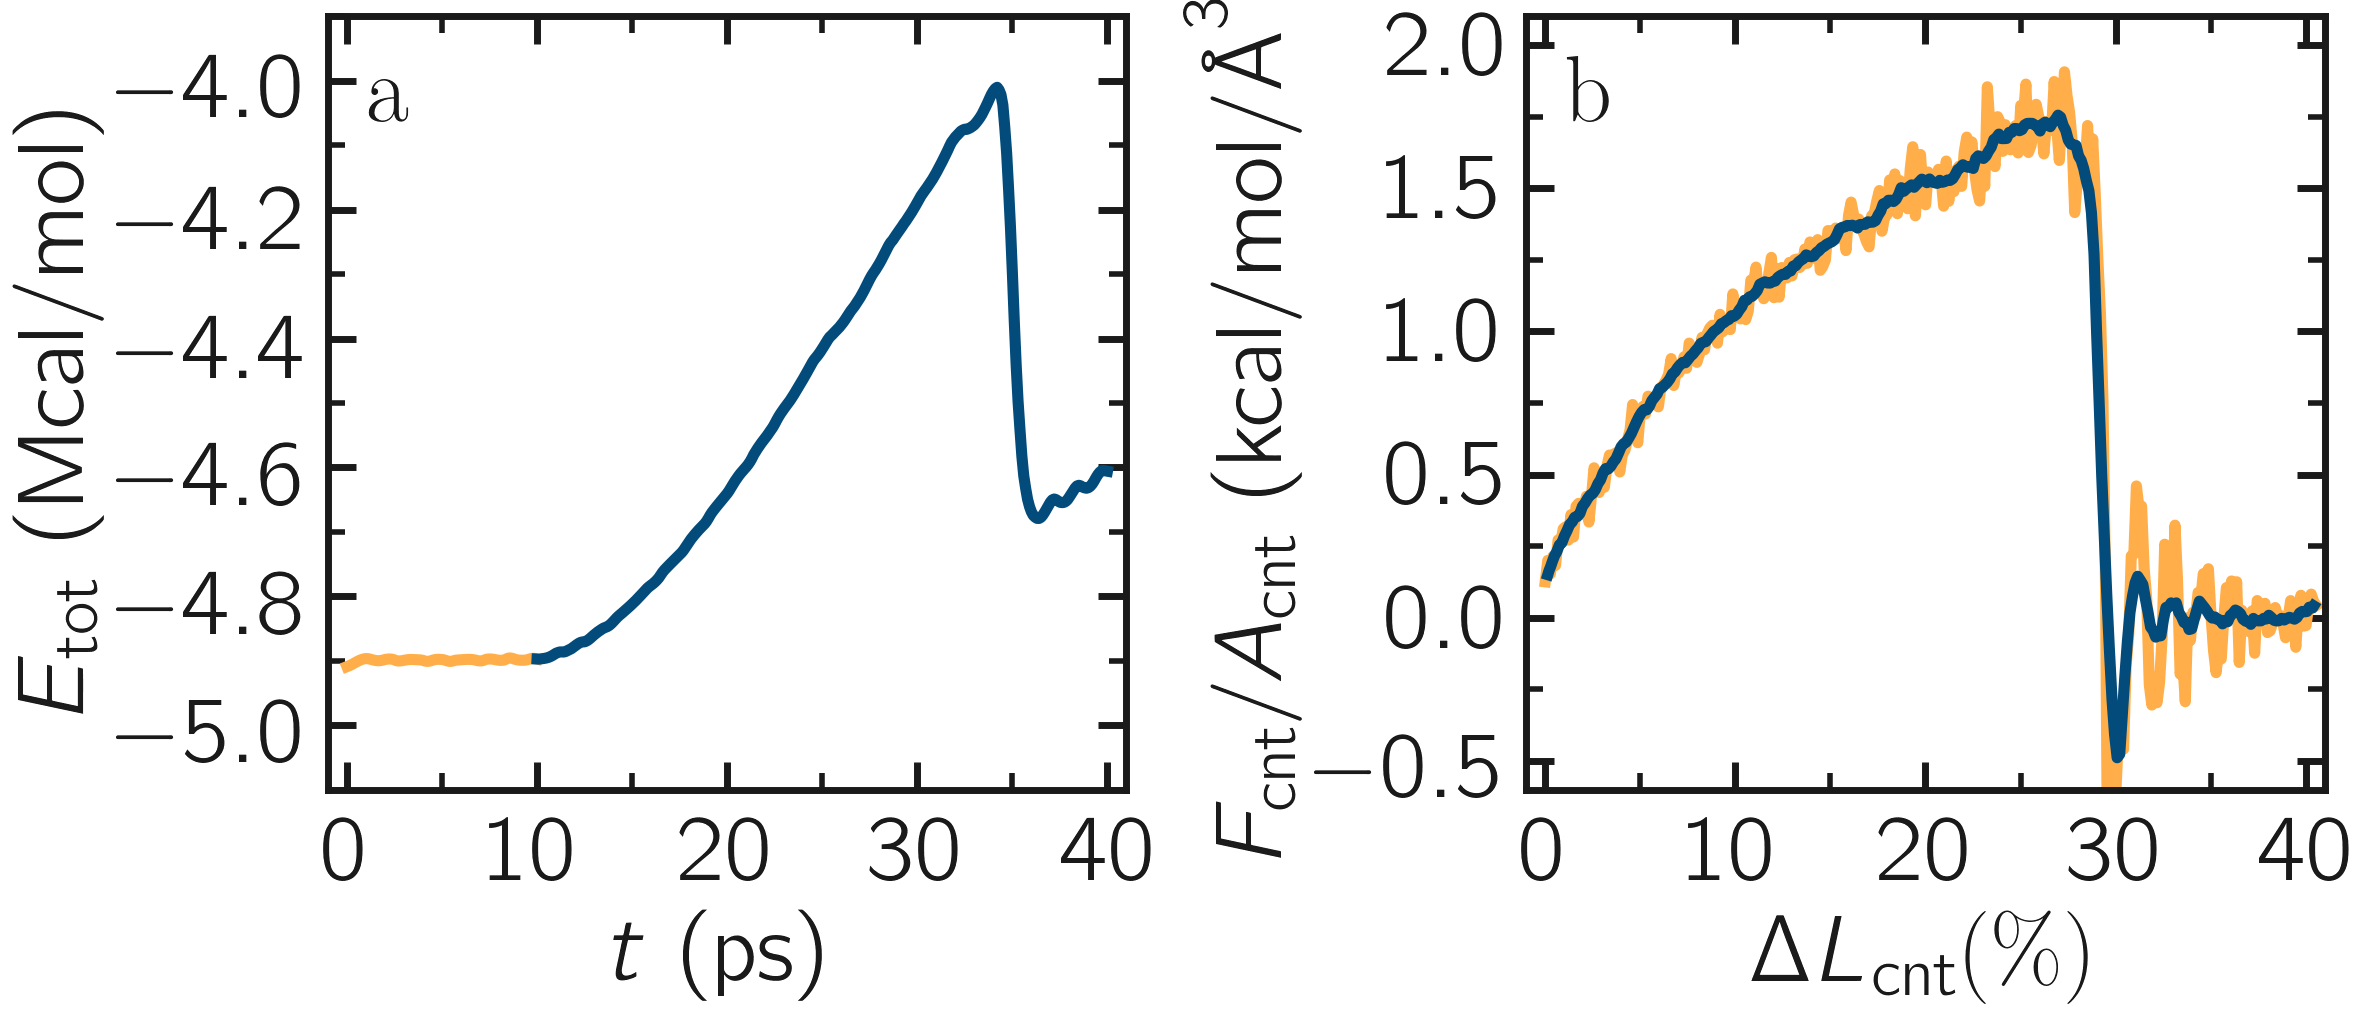
\includegraphics[width=\linewidth]{CNT-breakable-stress-energy}
\caption{a) Evolution of the total energy $E_\text{tot}$ of the CNT with time $t$.
b) Stress applied on the CNT during deformation, $F_\text{cnt}/A_\text{cnt}$,
where $F_\text{cnt}$ is the force and $A_\text{cnt}$ the CNT surface area,
as a function of the strain, $\Delta L_\text{cnt} = (L_\text{cnt}-L_\text{cnt-0}/L_\text{cnt-0})$, where
$L_\text{cnt}$ is the CNT length and $L_\text{cnt-0}$ the CNT initial length,
as simulated during \hyperref[carbon-nanotube-label]{Tutorial 2}.
Here, the potential is AIREBO, and the CNT is breakable.}
\label{fig:CNT-breakable-energy-stress}
\end{figure}

\paragraph{Tip: bonds representation with AIREBO}

In the following input file,
\href{\filepath tutorial2/breakable-with-tip.lmp}{\dwlcmd{breakable-with-tip.lmp}},
a trick is used to represent bonds while using AIREBO.  A detailled
explanation of the script is beyong the scope of the present tutorial.
In short, the trick is to use AIREBO with the molecular atom
style, and use the \lmpcmd{bond/break} command to update the status of the bonds
during the simulation:
\begin{lstlisting}
fix break all bond/break 1000 1 2.5
\end{lstlisting}
% S.G.: we could write a bit more about it

\subsection{Tutorial 3: Polymer in water}
\label{all-atoms-label}

\begin{figure}
\centering
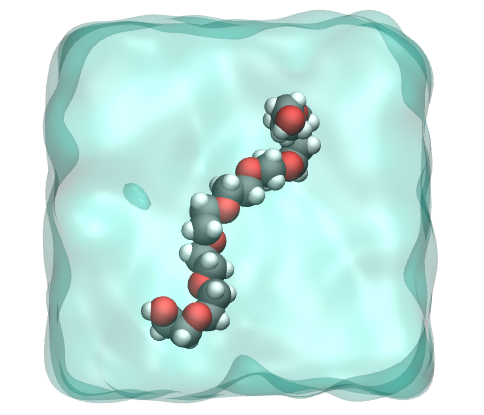
\includegraphics[width=0.55\linewidth]{PEG}
\caption{The polymer molecule (PEG - PolyEthylene Glycol) solvated in water as
simulated during \hyperref[all-atoms-label]{Tutorial 3}. Water molecules are
represented as a transparent continuum field for clarity.}
\label{fig:PEG}
\end{figure}

\noindent The goal of this tutorial is to use LAMMPS to solvate a small hydrophilic
polymer (PEG - PolyEthylene Glycol) in a reservoir of water (Fig.\,\ref{fig:PEG}).
Once the water reservoir is properly equilibrated at the desired temperature and
pressure, the polymer molecule is added and a constant stretching force is applied
to both ends of the polymer. The evolution of the polymer length is measured as
a function of time. The GROMOS 54A7 force field \cite{schmid2011definition} is used
for the PEG, the SPC/Fw model \cite{wu2006flexible} is used for the water, and the
long-range Coulomb interactions are solved using the PPPM solver \cite{luty1996calculating}.
This tutorial was inspired by a publication by Liese and coworkers, in which molecular
dynamics simulations are compared with force spectroscopy experiments \cite{liese2017hydration}.

\subsubsection{Preparing the water reservoir}

In this tutorial, the water reservoir is first prepared in the absence of the polymer.
A rectangular box of water is created and equilibrated at ambient temperature and
pressure.  The SPC/Fw water model is used \cite{wu2006flexible}, which is
a flexible variant of the rigid SPC (simple point charge) model \cite{berendsen1981interaction}.
To set up this tutorial, select \guicmd{Start Tutorial 3} from the
\guicmd{Tutorials} menu of LAMMPS--GUI and follow the instructions.
The editor should display the following content corresponding to \flecmd{water.lmp}:
\begin{lstlisting}
units real
atom_style full
bond_style harmonic
angle_style harmonic
dihedral_style harmonic
pair_style lj/cut/coul/long 10
kspace_style ewald 1e-5
special_bonds lj 0.0 0.0 0.5 coul 0.0 0.0 1.0 angle yes
\end{lstlisting}
With the unit style \lmpcmd{real}, masses are in grams per mole, distances in
Ångströms, time in femtoseconds, and energies in kcal/mole. With the \lmpcmd{atom\_style full},
each atom is a dot with a mass and a charge that can be linked by bonds, angles,
dihedrals, and/or impropers.  The \lmpcmd{bond\_style},
\lmpcmd{angle\_style}, and \lmpcmd{dihedral\_style} commands define the potentials
for the bonds, angles, and dihedrals used in the simulation, here \lmpcmd{harmonic}.
With the \lmpcmd{pair\_style} named \lmpcmd{lj/cut/coul/long}, atoms interact through
both a Lennard-Jones (LJ) potential and Coulomb interactions.  The value of $10\,\text{\AA{}}$ is the cutoff,
and the \lmpcmd{ewald} command defines the long-range solver for the Coulomb
interactions \cite{ewald1921berechnung}.  Finally, the \lmpcmd{special\_bonds} command, which was already seen in
\hyperref[carbon-nanotube-label]{tutorial 2}, sets the LJ and Coulomb weighting
factors for the interaction between neighboring atoms.

Let us create a 3D simulation box of dimensions $6 \times 3 \times 3 \; \text{nm}^3$,
and make space for 8 atom types (2 for the water, 6 for the polymer), 7 bond types
(1 for the water, 6 for the polymer), 8 angle types (1 for the water, 7 for the polymer),
and 4 dihedral types (only for the polymer). Copy the following lines into \flecmd{water.lmp}:
\begin{lstlisting}
 region box block -30 30 -15 15 -15 15
 create_box 8 box &
 bond/types 7 &
 angle/types 8 &
 dihedral/types 4 &
 extra/bond/per/atom 3 &
 extra/angle/per/atom 6 &
 extra/dihedral/per/atom 10 &
 extra/special/per/atom 14
\end{lstlisting}
The \lmpcmd{extra/x/per/atom} commands are here for
memory allocation.  We will use a file named
\href{\filepath tutorial3/parameters.inc}{\dwlcmd{parameters.inc}} that contains
all the parameters (masses, interaction energies, bond equilibrium
distances, etc).  In \flecmd{water.lmp}, add the following line:
\begin{lstlisting}
include parameters.inc
\end{lstlisting}

\begin{note}
This tutorial uses type labels \cite{typelabel_paper} to map each of the
numeric atom types with a string (see the \flecmd{parameters.inc} file):
\begin{lstlisting}
labelmap atom 1 OE 2 C 3 HC 4 H 5 CPos 6 OAlc 7 OW 8 HW
\end{lstlisting}
Therefore, the oxygen and hydrogen atoms of water (respectively types 7 and 8)
can be referred to as `OW' and `HW', respectively.  Similar maps are used for 
the bond types, angle types, and dihedral types.
\end{note}

Let us create water molecules. To do so, let us import a molecule template called
\flecmd{water.mol} and then randomly create 700 molecules.  Add the following
lines into \flecmd{water.lmp}:
\begin{lstlisting}
molecule h2omol water.mol
create_atoms 0 random 700 87910 NULL mol h2omol 454756 &
  overlap 1.0 maxtry 50
\end{lstlisting}
The \lmpcmd{overlap 1.0} option of the \lmpcmd{create\_atoms} command ensures
that no atoms are placed exactly in the same position, as this would cause the
simulation to crash. The \lmpcmd{maxtry 50} asks LAMMPS to try at most 50 times
to insert the molecules, which is useful in case some insertion attempts are
rejected due to overlap.  In some cases, depending on the system and the values
of \lmpcmd{overlap} and \lmpcmd{maxtry}, LAMMPS may not create the desired number
of molecules.  Always check the number of created atoms in the \lmpcmd{log} file
(or in the \guicmd{Output} window), where you should see:
\begin{lstlisting}
Created 2100 atoms
\end{lstlisting}
When LAMMPS fails to create the desired number of molecules, a WARNING appears.
The molecule template called \href{\filepath tutorial3/water.mol}{\dwlcmd{water.mol}}
must be downloaded and saved next to \lmpcmd{water.lmp}.  This template contains
the necessary structural information of a water molecule, such as the number of
atoms, or the IDs of the atoms that are connected by bonds and angles.

Then, let us organize the atoms of types OW and HW of the water molecules in a
group named \textit{H2O} and perform a small energy minimization. The energy
minimization is mandatory here given the small \textit{overlap} value of 1 Ångstrom
chosen in the \textit{create\_atoms} command. Add the following lines into \flecmd{input.lmp}:
\begin{lstlisting}
 group H2O type OW HW
 minimize 1.0e-4 1.0e-6 100 1000
 reset_timestep 0
\end{lstlisting}
In general, resetting the step of the simulation to 0 using the
\textit{reset\_timestep} command is optional.
It is used here because the number of iterations performed by the \textit{minimize}
command is usually not a round number (since the minimization stops when one of
four criteria is reached). Let us use the \textit{fix npt} to control the temperature
of the molecules with a Nosé-Hoover thermostat and the pressure of the system with
a Nosé-Hoover barostat \cite{nose1984unified, hoover1985canonical, martyna1994constant},
by adding the following line into \flecmd{input.lmp}:
\begin{lstlisting}
 fix mynpt all npt temp 300 300 100 &
     iso 1 1 1000
\end{lstlisting}
The \textit{fix npt} allows us to impose both a temperature of $300\,\text{K}$
(with a damping constant of $100\,\text{fs}$), and a pressure of 1 atmosphere
(with a damping constant of $1000\,\text{fs}$). With the \textit{iso} keyword,
the three dimensions of the box will be re-scaled simultaneously.

Let us output the system into images by adding the following commands to \flecmd{input.lmp}:
\begin{lstlisting}
 dump mydmp all image 1000 dump.*.ppm type &
     type shiny 0.1 box no 0.01 &
     view 0 90 zoom 1.8
 dump_modify mydmp backcolor white &
   acolor OW red acolor HW white &
   adiam OW 3 adiam HW 1.5
\end{lstlisting}
Let us also extract the volume and density in the terminal every 1000 steps:
\begin{lstlisting}
 variable myvol equal vol
 variable myoxy equal count(H2O)/3
 variable myrho equal ${myoxy}/v_myvol
 thermo 1000
 thermo_style custom step temp etotal &
     v_myvol v_myrho
\end{lstlisting}
The variable \textit{myoxy} corresponds to the number of atoms divided by 3, i.e.
the number of molecules, and the variable \textit{myrho} is the number of molecules
divided by the volume of the simulation box, i.e.~the density (in $\mathrm{\AA{}}^{-3}$).

Finally, let us set the timestep to 1.0 fs, and run the simulation for 20 ps by
adding the following lines into \flecmd{input.lmp}:
\begin{lstlisting}
 timestep 1.0
 run 20000

 write_data H2O.data
\end{lstlisting}
% S.G. may be a binary restart file could be used here to illustrate the new functionalities of the GUI?
The final state is written into \flecmd{H2O.data}. From the value of \textit{myrho},
it should be clear that the system is quickly reaching its equilibrium
density (see a snapshot of the equilibrated system in Fig.\,\ref{fig:PEG-water},
and the evolution of the density in Fig.\,\ref{fig:PEG-density}).

\begin{figure}
\centering
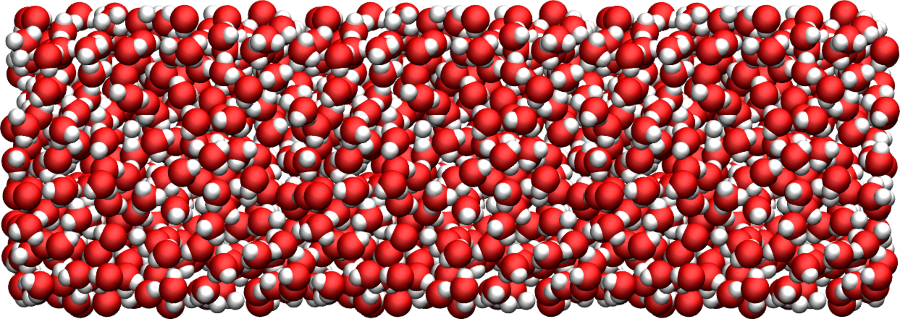
\includegraphics[width=\linewidth]{PEG-water}
\caption{Water reservoir after equilibration. Oxygen atoms are in red, and hydrogen
atoms are in white.}
\label{fig:PEG-water}
\end{figure}

\begin{figure}
\centering
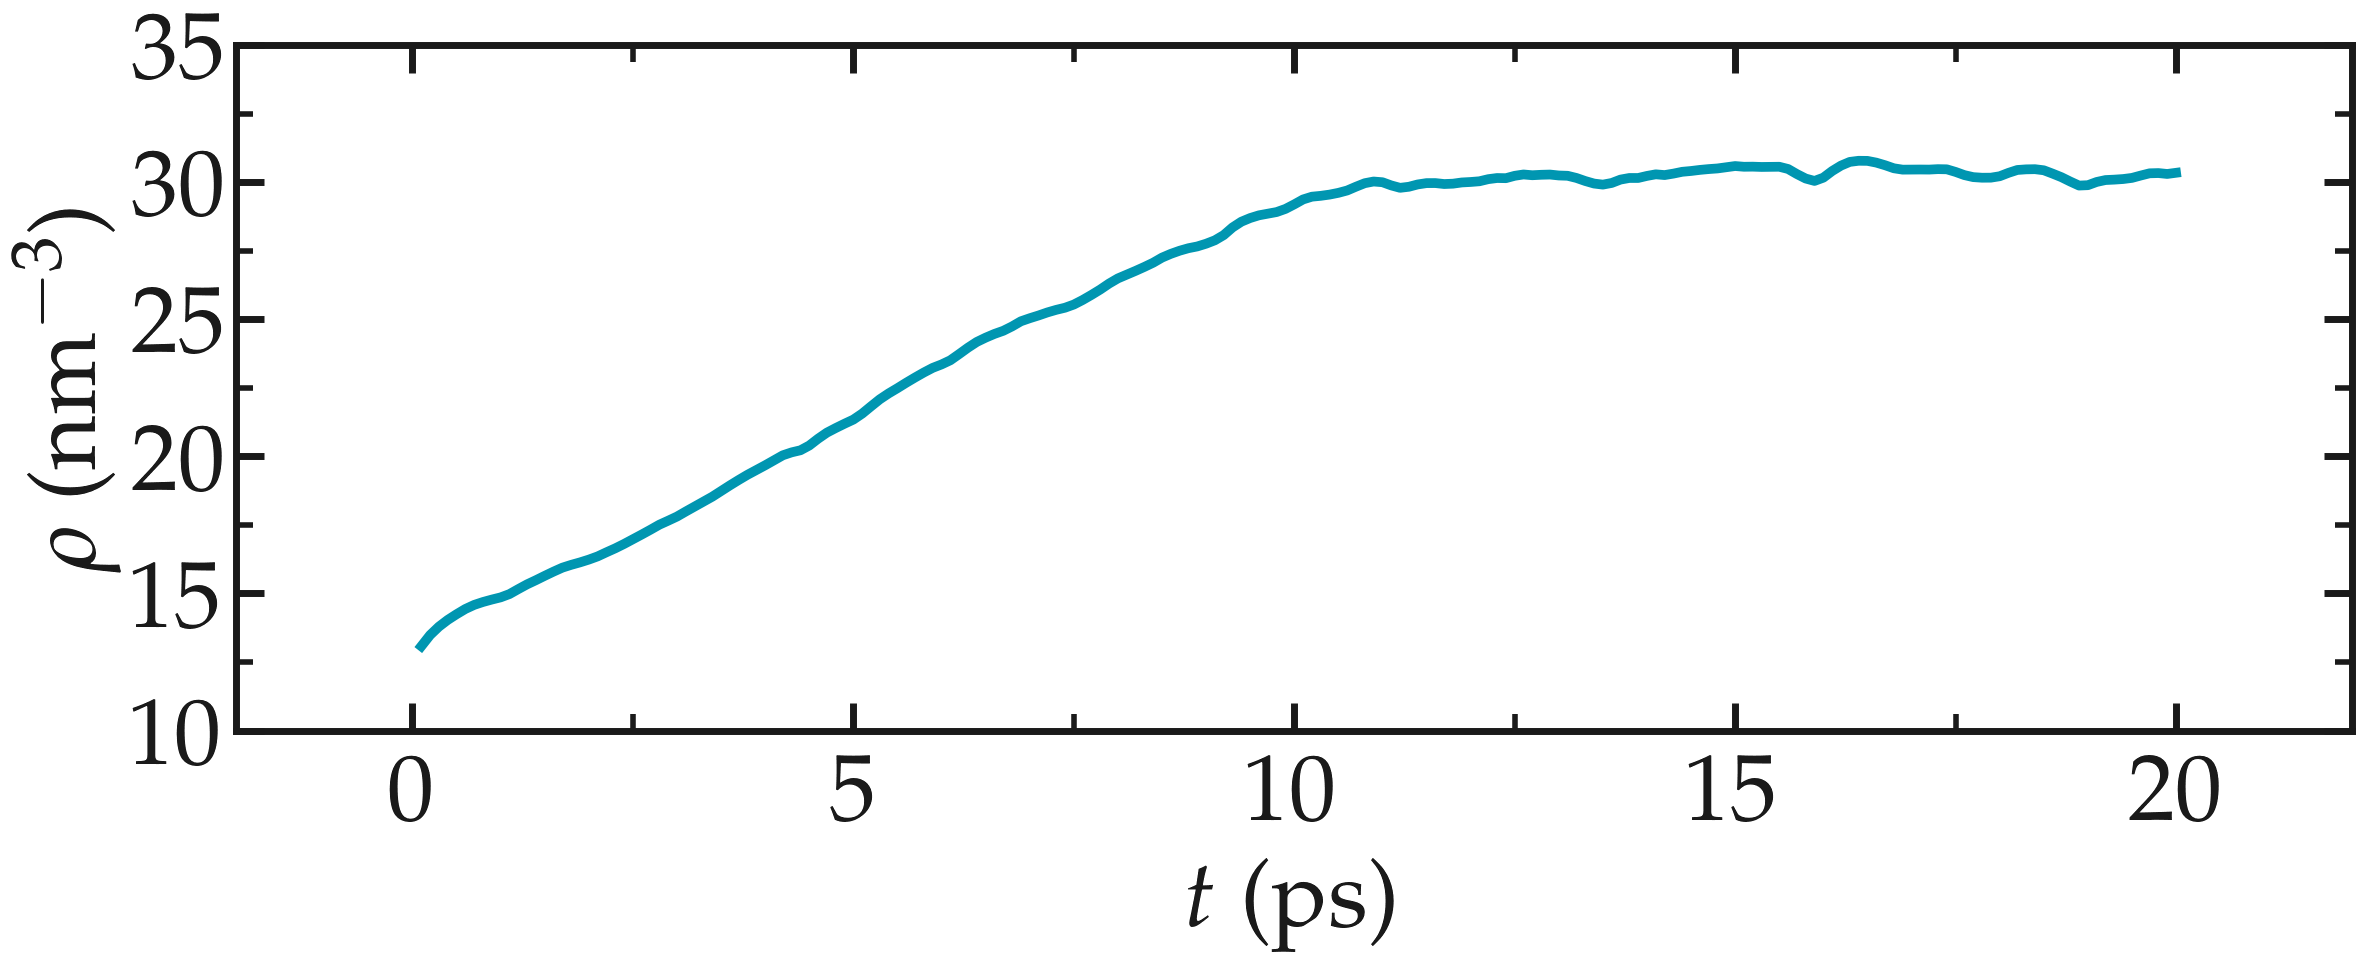
\includegraphics[width=\linewidth]{PEG-density}
\caption{Evolution of the density $\rho$ of water with time $t$. The density
quickly reaches a plateau.}
\label{fig:PEG-density}
\end{figure}

\subsubsection{Solvating the PEG in water}
Now that the water reservoir is equilibrated, we can safely include the PEG polymer
in the water. The PEG molecule topology was downloaded from the ATB repository
\cite{malde2011automated, oostenbrink2004biomolecular}. It has a formula
$\text{C}_{28}\text{H}_{58}\text{O}_{15}$, and the parameters are taken from
the GROMOS 54A7 force field \cite{schmid2011definition}.

\begin{figure}
\centering
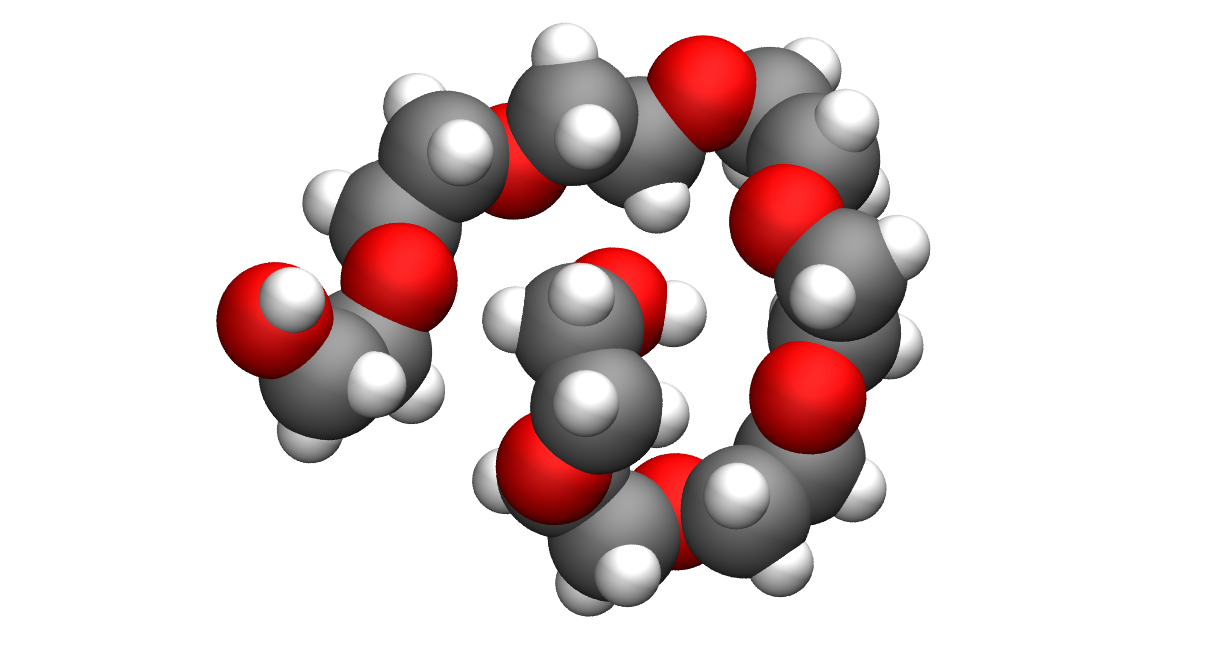
\includegraphics[width=\linewidth]{PEG-in-vacuum}
\caption{The PEG molecule in vacuum. The carbon atoms are in gray, the oxygen
atoms in red, and the hydrogen atoms in white.}
\label{fig:PEG-in-vacuum}
\end{figure}

Create a second folder alongside \flrcmd{pureH2O/} and call it \flrcmd{mergePEGH2O/}.
Create a new blank file in it, call it \flecmd{input.lmp}. Within \flecmd{input.lmp},
copy the same first lines as previously:
\begin{lstlisting}
 units real
 atom_style full
 bond_style harmonic
 angle_style harmonic
 dihedral_style harmonic
 pair_style lj/cut/coul/long 10
 kspace_style pppm 1e-5
 special_bonds lj 0.0 0.0 0.5 coul 0.0 0.0 1.0 &
     angle yes dihedral yes
\end{lstlisting}
Then, import the previously generated data file \flecmd{H2O.data} as well as the \flecmd{PARM.lmp} file:
\begin{lstlisting}
 read_data ../pureH2O/H2O.data &
     extra/bond/per/atom 3 &
     extra/angle/per/atom 6 &
     extra/dihedral/per/atom 10 &
     extra/special/per/atom 14
 include ../PARM.lmp
\end{lstlisting}
Download the template called
\href{\filepath tutorial3/mergePEGH2O/PEG-GROMOS.mol}{\dwlcmd{PEG-GROMOS.mol}}
for the PEG molecule, and then create a single molecule in the middle of the box:
\begin{lstlisting}
 molecule pegmol PEG-GROMOS.mol
 create_atoms 0 single 0 0 0 mol pegmol 454756
\end{lstlisting}
Let us create 2 groups to differentiate the PEG from the H2O, by adding the following
lines into \flecmd{input.lmp}:
\begin{lstlisting}
 group H2O type OW HW
 group PEG type C CPos H HC OAlc OE
\end{lstlisting}
Water molecules that are overlapping with the PEG must be deleted to avoid future crashing.
Add the following line into \flecmd{input.lmp}:
\begin{lstlisting}
 delete_atoms overlap 2.0 H2O PEG mol yes
\end{lstlisting}
Here the value of 2 Ångströms for the overlap cutoff was fixed arbitrarily and can
be chosen through trial and error. If the cutoff is too small, the simulation will
crash. If the cutoff is too large, too many water molecules will unnecessarily be
deleted.

Finally, let us use the \textit{fix npt} to control the temperature, as
well as the pressure by allowing the box size to be rescaled along the \textit{x} axis:
\begin{lstlisting}
 fix mynpt all npt temp 300 300 100 x 1 1 1000
 timestep 1.0
\end{lstlisting}
Once more, let us create images of the systems:
\begin{lstlisting}
 dump mydmp all image 1000 dump.*.ppm type &
     type shiny 0.1 box no 0.01 &
     view 0 90 zoom 1.8  fsaa yes bond atom 0.8
 dump_modify mydmp backcolor white &
     acolor OW red acolor HW white &
     acolor OE red acolor OAlc red &
     acolor C gray acolor CPos gray &
     acolor H white acolor HC white &
     adiam OW 0.2 adiam HW 0.2 &
     adiam C 3 adiam CPos 3 adiam OAlc 2.8 &
     adiam H 1 adiam HC 1 adiam OE 2.8
 thermo 1000
\end{lstlisting}
Finally, let us perform a short equilibration and print the
final state in a data file. Add the following lines to the data file:
\begin{lstlisting}
 run 30000
 write_data mix.data
\end{lstlisting}
From the outputs, you can make sure that the temperature remains close to the
target value of $300~\text{K}$ throughout the entire simulation, and the that
the volume and total energy are almost constant, suggesting
that the system was close to equilibrium from the start. See a snapshot of the
system in Fig.\,\ref{fig:PEG-solvated}.

\begin{figure}
\centering
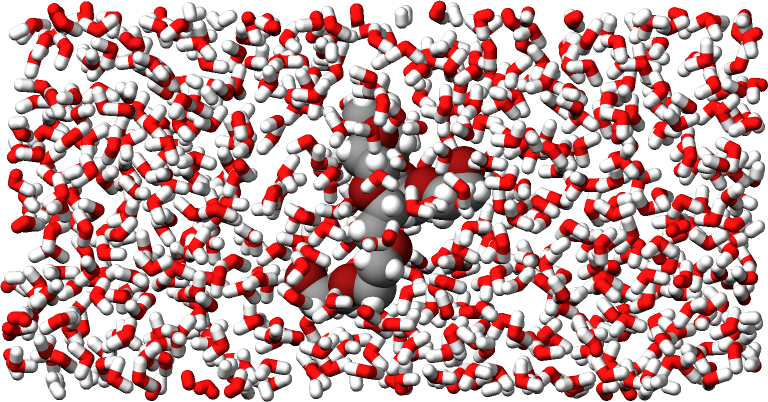
\includegraphics[width=\linewidth]{PEG-solvated}
\caption{A single PEG molecule in water. Water molecules are represented as a
transparent continuum field for clarity.}
\label{fig:PEG-solvated}
\end{figure}

\subsubsection{Stretching the PEG molecule}
Here, a constant forcing is applied to the two ends of the PEG molecule until it
stretches. Create a new folder next to the previously created folders, call it
\flrcmd{pullonPEG/}, and create a new input file in it called \flecmd{input.lmp}.
First, let us create a variable \textit{f0} corresponding to the magnitude of the
force we are going to apply. Copy the following line into the \flecmd{input.lmp} file:
\begin{lstlisting}
variable f0 equal 5
\end{lstlisting}
The force magnitude of $1\,\text{kcal/mol/\AA{}}$ corresponds to $67.2\,\text{pN}$
and was chosen to be large enough to overcome the thermal agitation and the entropic
contribution from both water and PEG molecules (it was chosen by trial and error).
Then, copy the same lines as previously:
\begin{lstlisting}
 units real
 atom_style full
 bond_style harmonic
 angle_style harmonic
 dihedral_style harmonic
 pair_style lj/cut/coul/long 10
 kspace_style pppm 1e-5
 special_bonds lj 0.0 0.0 0.5 &
     coul 0.0 0.0 1.0 &
     angle yes dihedral yes
\end{lstlisting}
Start the simulation from the equilibrated PEG-water system and include again the
parameter file by adding the following lines to the \flecmd{input.lmp}:
\begin{lstlisting}
 read_data ../mergePEGH2O/mix.data
 include ../PARM.lmp
\end{lstlisting}
Next, let us create some useful atom groups, including H2O and PEG (as previously),
as well as 2 groups containing a single atom each, the oxygen atoms at the ends
of the chain. Atoms of types OAlc correspond to the hydroxy (alcohol) group oxygen
atoms located at the ends of the PEG molecule, which we are going to use to pull
on the PEG molecule. Add the following lines to the \flecmd{input.lmp}:
\begin{lstlisting}
 group H2O type OW HW
 group PEG type C CPos H HC OAlc OE
 group ends type OAlc
 variable xcm equal xcm(ends,x)
 variable oxies atom type==label2type(atom,OAlc)
 variable end1 atom v_oxies*(x>v_xcm)
 variable end2 atom v_oxies*(x<v_xcm)
 group topull1 variable end1
 group topull2 variable end2
\end{lstlisting}
Add the following \textit{dump} command to create images of the system:
\begin{lstlisting}
 dump mydmp all image 1000 dump.*.ppm type &
     type shiny 0.1 box no 0.01 &
     view 0 90 zoom 1.8 fsaa yes bond atom 0.8
 dump_modify mydmp backcolor white &
     acolor OW red acolor HW white &
     acolor OE red acolor OAlc red &
     acolor C gray acolor CPos gray &
     acolor H white acolor HC white &
     adiam OW 0.2 adiam HW 0.2 &
     adiam C 3 adiam CPos 3 adiam OAlc 2.8 &
     adiam H 1 adiam HC 1 adiam OE 2.8
\end{lstlisting}
Let us use a single Nosé-Hoover thermostat applied to all the atoms by adding the
following lines to \flecmd{input.lmp}:
\begin{lstlisting}
timestep 1.0
fix mynvt all nvt temp 300 300 100
\end{lstlisting}
Let us also print the end-to-end distance of the PEG,
here defined as the distance between the groups \textit{topull1}
and \textit{topull2}, as well as the gyration
radius of the molecule \cite{fixmanRadiusGyrationPolymer1962a}
by adding the following lines to \flecmd{input.lmp}:
\begin{lstlisting}
 variable x1 equal xcm(topull1,x)
 variable x2 equal xcm(topull2,x)
 variable y1 equal xcm(topull1,y)
variable y2 equal xcm(topull2,y)
 variable z1 equal xcm(topull1,z)
 variable z2 equal xcm(topull2,z)
 variable delta_r equal &
     sqrt((v_x1-v_x2)^2+(v_y1-v_y2)^2 &
     +(v_z1-v_z2)^2)
 compute rgyr PEG gyration
 thermo_style custom step temp etotal v_delta_r c_rgyr
 thermo 1000
\end{lstlisting}
Finally, let us simulate 30 picoseconds without any external forcing:
\begin{lstlisting}
 run 30000
\end{lstlisting}
This first run will serve as a benchmark to quantify later the changes induced
by the forcing. Then, let us apply a forcing on the 2 selected oxygen atoms using two
\textit{add\_force} commands, and run for an extra 30 ps:
\begin{lstlisting}
 fix myaf1 topull1 addforce ${f0} 0 0
 fix myaf2 topull2 addforce -${f0} 0 0
 run 30000
\end{lstlisting}
Run the \flecmd{input.lmp} file using LAMMPS. From the generated images of the system,
you should see that the PEG molecule eventually aligns
in the direction of the force (as seen in Fig.\,\ref{fig:PEG-in-water}).
The evolutions of the end-to-end distance and of the gyration radius over
time show that the PEG is adjusting to the external forcing in less than
$10~\text{ps}$ (Fig.\,\ref{fig:PEG-distance}).

\begin{figure}
\centering
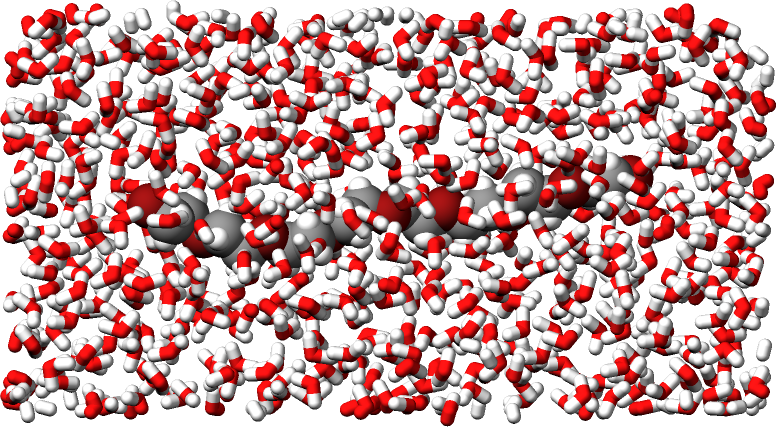
\includegraphics[width=\linewidth]{PEG-in-water}
\caption{PEG molecule stretched along the $x$ direction in water. Water molecules
are represented as a transparent continuum field for clarity.}
\label{fig:PEG-in-water}
\end{figure}

\begin{figure}
\centering
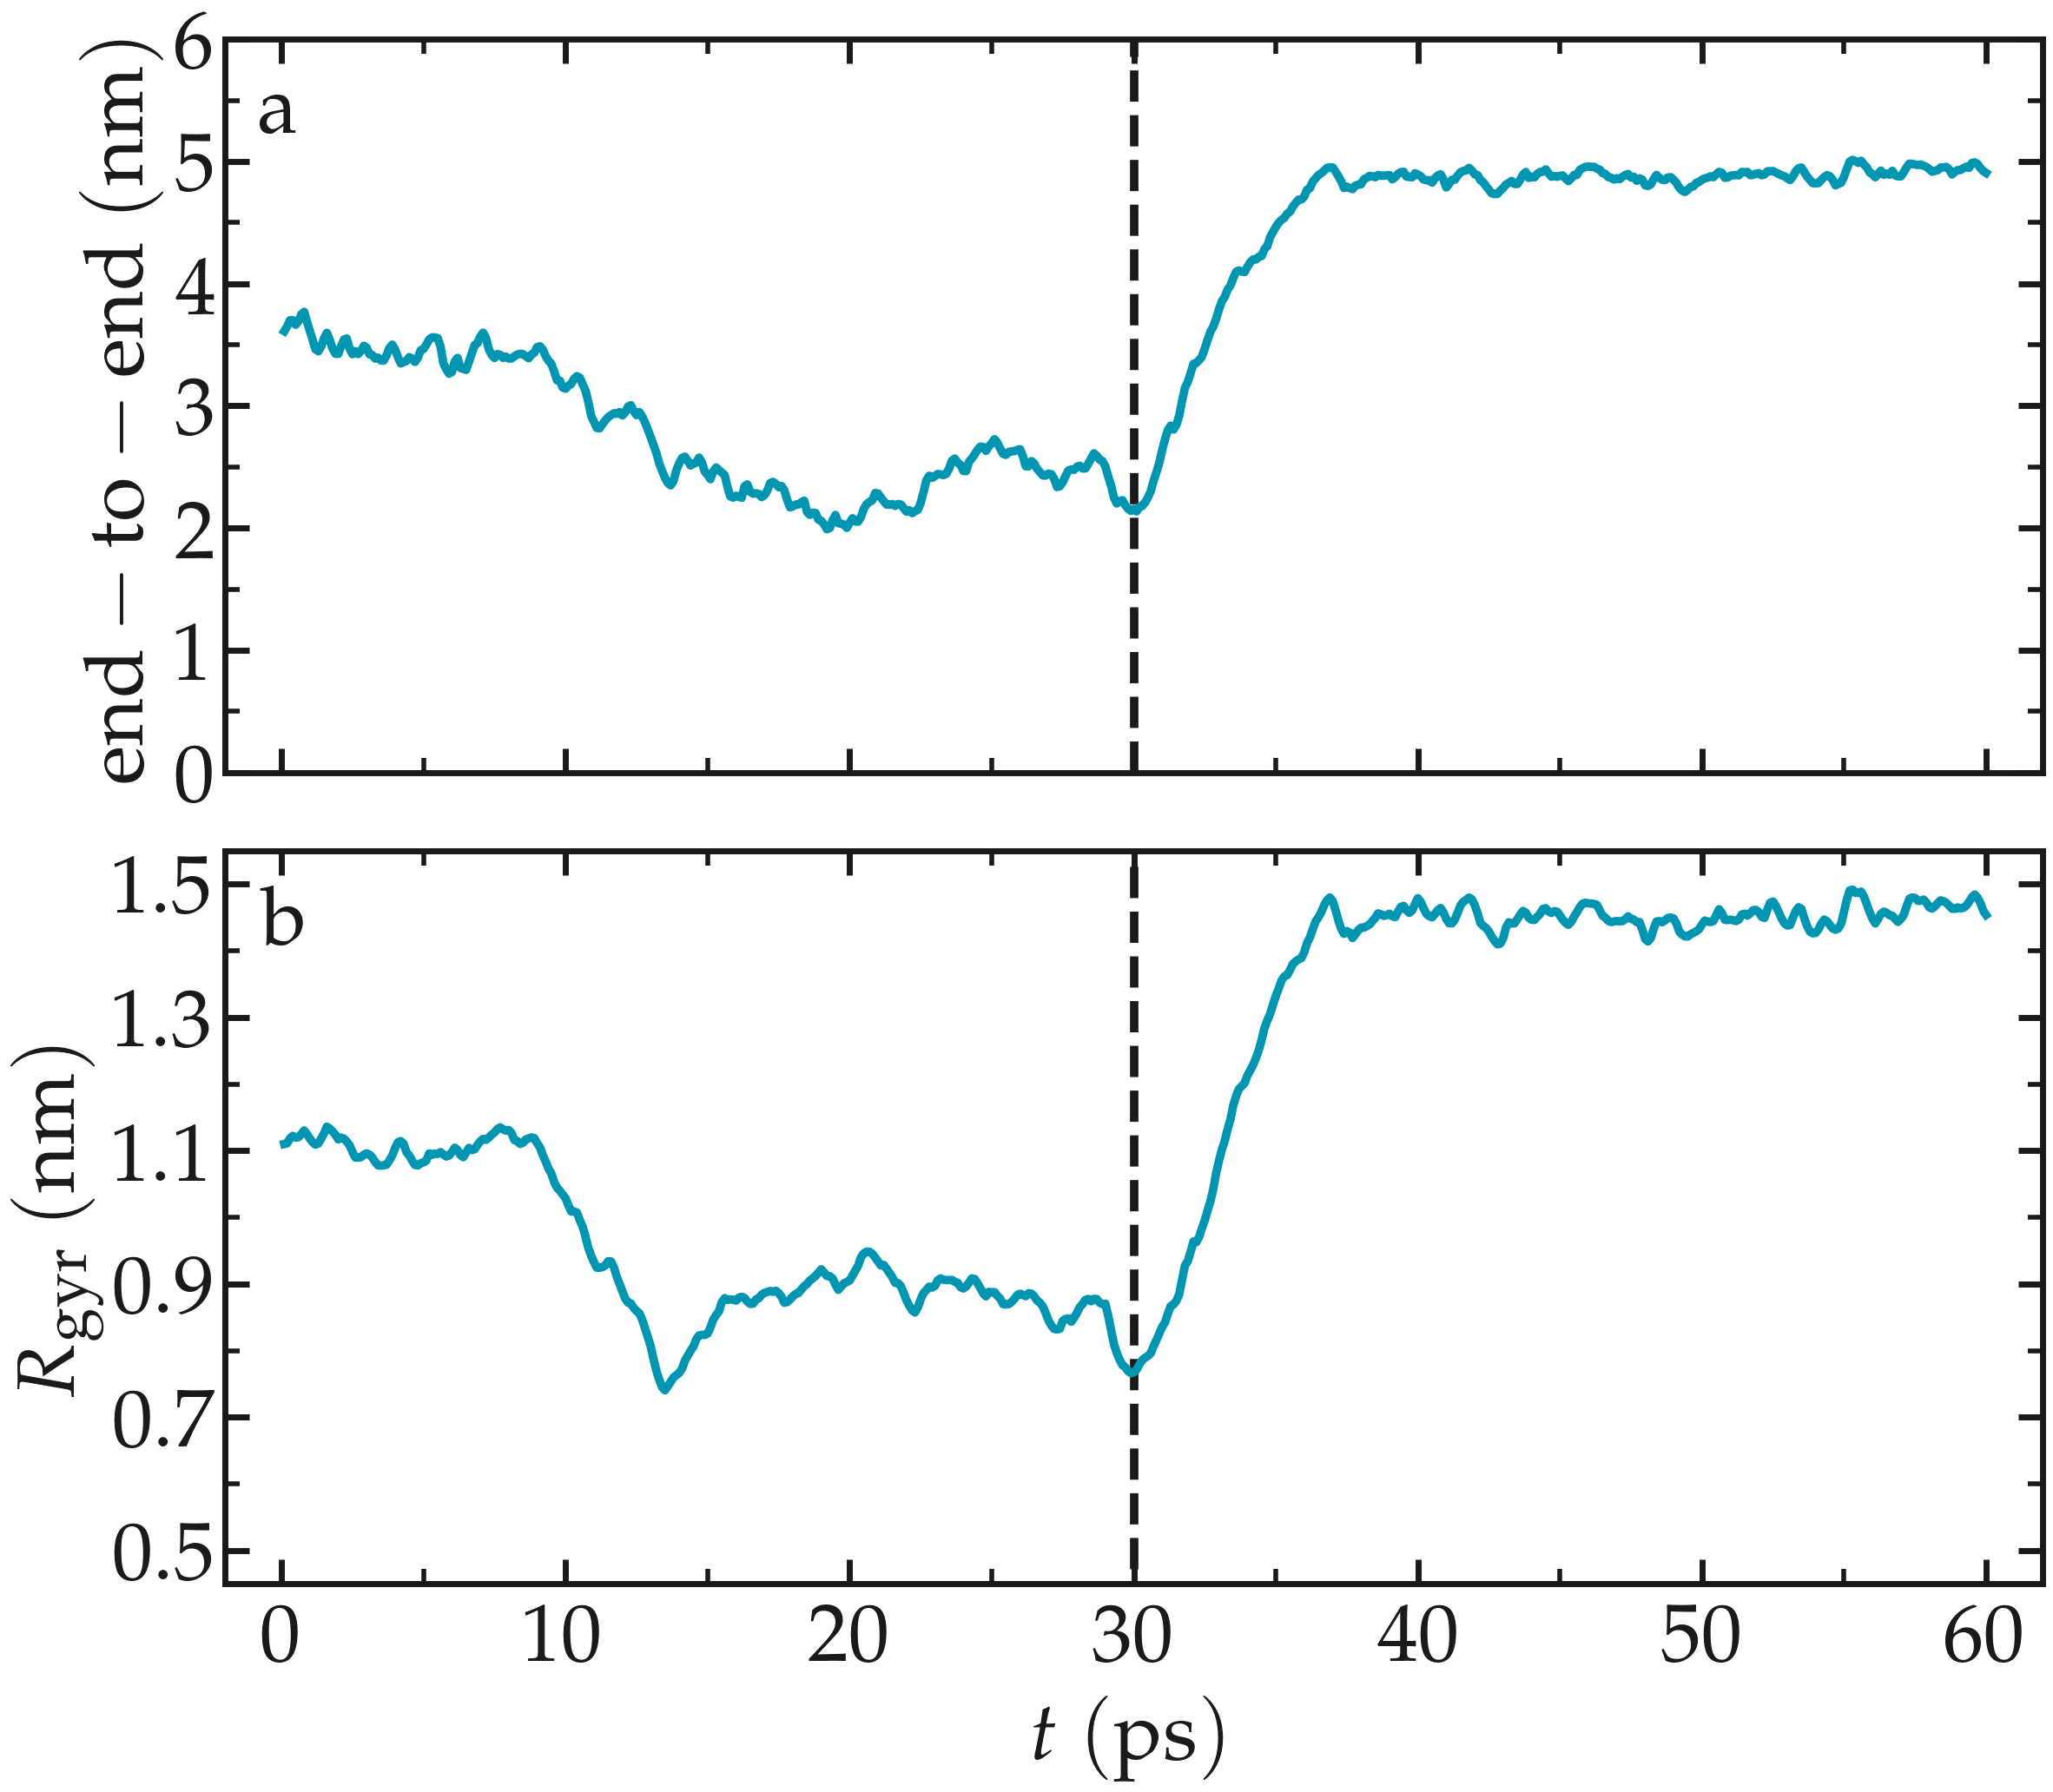
\includegraphics[width=\linewidth]{PEG-distance}
\caption{a) Evolution of the end-to-end distance $d_\text{end-to-end}$ of the
PEG with time $t$. The forcing starts at $t = 5\,\text{ps}$. b) Evolution of
the gyration radius $R_\text{gyr}$ of the PEG molecule.}
\label{fig:PEG-distance}
\end{figure}

\subsection{Tutorial 4: Nanosheared electrolyte}
\label{sheared-confined-label}

\begin{figure}
\centering
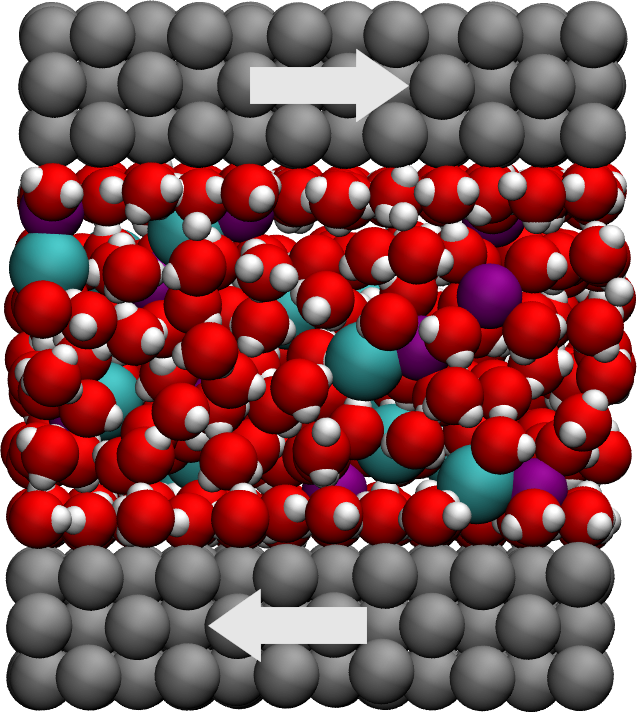
\includegraphics[width=0.55\linewidth]{NANOSHEAR}
\caption{The electrolyte confined in a nanometer slit pore as simulated during
\hyperref[sheared-confined-label]{Tutorial 4}. $\text{Na}^+$ ions are represented
as purple spheres, $\text{Cl}^-$ ions as cyan spheres, water molecules are colored
in red and white, and the walls are colored in gray. The arrows indicate the
imposed lateral motion of the walls.}
\label{fig:NANOSHEAR}
\end{figure}

\noindent The objective of this tutorial is to simulate an electrolyte
nanoconfined and sheared by two walls (Fig.\,\ref{fig:NANOSHEAR}). The density
and velocity profiles of the fluid in the direction normal to the walls are
extracted to highlight the effect of confining a fluid on its local properties.
This tutorial illustrates some key aspects of combining a fluid and a solid in
the same simulation. A major difference from the previous tutorial,
\hyperref[all-atoms-label]{Polymer in water}, is that here a rigid four-point
water model named TIP4P is used \cite{abascal2005general}. TIP4P is one of
the most common water models due to its high accuracy.

\subsubsection{System preparation}
The fluid and walls must first be generated and then equilibrated at a reasonable
temperature and pressure.

\paragraph{System generation}
Create a new folder called \flrcmd{systemcreation/}. Within
\flrcmd{systemcreation/}, open a blank file called \flecmd{input.lmp}, and
copy the following lines into it:
\begin{lstlisting}
boundary p p f
units real
atom_style full
bond_style harmonic
angle_style harmonic
pair_style lj/cut/tip4p/long O H O-H H-O-H &
    0.1546 12.0
kspace_style pppm/tip4p 1.0e-4
kspace_modify slab 3.0
\end{lstlisting}

These lines are used to define the most basic parameters, including the
\textit{atom}, \textit{bond}, and \textit{angle} styles, as well as interaction
potential. Here, \textit{lj/cut/tip4p/long} imposes a Lennard-Jones potential with
a cut-off at $12\,\text{$\text{\AA{}}$}$ and a long-range Coulomb potential.

% S.G. To fix, this was removed from tutorial 3 : The \textit{pppm} style refers to particle-particle particle-mesh . \cite{luty1996calculating}
So far, the commands are relatively similar to those in the previous tutorial,
\hyperref[all-atoms-label]{Polymer in water}, with two major differences: the use
of \textit{lj/cut/tip4p/long} instead of \textit{lj/cut/coul/long}, and \textit{pppm/tip4p}
instead of \textit{pppm}. When using \textit{lj/cut/tip4p/long} and \textit{pppm/tip4p},
the interactions resemble the conventional Lennard-Jones and Coulomb interactions,
except that they are specifically designed for the four-point water model. Therefore,
LAMMPS automatically creates a four-point water molecule using atoms of type O as
oxygen and atoms of type H as hydrogen. The fourth massless atom (\textit{M}) of the
TIP4P water molecule does not have to be defined explicitly, and the value of
$0.1546\,\text{$\text{\AA{}}$}$ corresponds to the \textit{O-M} distance of the
TIP4P-2005 water model \cite{abascal2005general}. All the other atoms in the simulation
are treated normally with long-range Coulomb interactions. Another novelty, here, is
the use of \textit{kspace\_modify slab 3.0} that is combined with the non-periodic
boundaries along the $z$ coordinate: \textit{boundary p p f}. With the \textit{slab}
option, the system is treated as periodical along $z$, but with an empty volume inserted
between the periodic images of the slab, and the interactions along $z$ effectively turned off.

Let us create the box by adding the following lines to \flecmd{input.lmp}:

\begin{lstlisting}
lattice fcc 4.04
region box block -3 3 -3 3 -5 5
create_box 5 box &
bond/types 1 &
angle/types 1 &
extra/bond/per/atom 2 &
extra/angle/per/atom 1 &
extra/special/per/atom 2
labelmap atom 1 O 2 H 3 Na+ 4 Cl- 5 WALL
labelmap bond 1 O-H
labelmap angle 1 H-O-H
\end{lstlisting}
The \textit{lattice} command defines the unit cell. Here, the face-centered cubic (fcc) lattice
with a scale factor of 4.04 has been chosen for the future positioning of the atoms
of the walls. The \textit{region} command defines a geometric region of space. By choosing
\textit{xlo=-3} and \textit{xhi=3}, and because we have previously chosen a lattice with a scale
factor of 4.04, the region box extends from $-12.12~\text{\AA{}}$ to $12.12~\text{\AA{}}$
along the $x$ direction. The \textit{create\_box} command creates a simulation box with
5 types of atoms: the oxygen and hydrogen of the water molecules, the two ions ($\text{Na}^+$,
$\text{Cl}^-$), and the atom of the walls. The \textit{create\_box} command extends over 6
lines thanks to the $\&$ character. The second and third lines are used to indicate that the
simulation contains 1 type of bond and 1 type of angle (both required by the water molecule).
The parameters for these bond and angle constraints will be given later. The three last
lines are for memory allocation. The \textit{labelmap} command assigns alphanumeric type labels
to each numeric atom type, bond type, and angle type.

Now, we can add atoms to the system. First, let us create two sub-regions corresponding
respectively to the two solid walls, and create a larger region from the union of the
two regions. Then, let us create atoms of type WALL within the two regions. Add the
following lines to \flecmd{input.lmp}:
\begin{lstlisting}
region rbotwall block -3 3 -3 3 -4 -3
region rtopwall block -3 3 -3 3 3 4
region rwall union 2 rbotwall rtopwall
create_atoms WALL region rwall
\end{lstlisting}
Atoms will be placed in the positions of the previously defined lattice, thus
forming fcc solids. To add the water molecules, first download the molecule
template called \href{\filepath tutorial4/RigidH2O.txt}{\dwlcmd{RigidH2O.txt}}
and place it within \flrcmd{systemcreation/}. The template contains all the
necessary information concerning the water molecule, such as atom positions,
bonds, and angles. Add the following lines to \flecmd{input.lmp}:
\begin{lstlisting}
region rliquid block INF INF INF INF -2 2
molecule h2omol RigidH2O.txt
create_atoms 0 region rliquid mol h2omol 482793
\end{lstlisting}
Within the last three lines, a \textit{region} named \textit{rliquid} is
created based on the last defined lattice, \textit{fcc 4.04}. \textit{rliquid}
will be used for depositing the water molecules. The \textit{molecule} command
opens up the molecule template called \flecmd{RigidH2O.txt}, and names the
associated molecule \textit{h2omol}. The new molecules are placed on the
\textit{fcc 4.04} lattice by the \textit{create\_atoms} command. The first
parameter is 0, meaning that the atom IDs from the \flecmd{RigidH2O.txt} file
will be used. The number \textit{482793} is a seed that is required by LAMMPS,
it can be any positive integer.

Finally, let us create 30 ions (15 $\text{Na}^+$ and 15 $\text{Cl}^-$) in between
the water molecules, by adding the following commands to \flecmd{input.lmp}:
\begin{lstlisting}
create_atoms Na+ random 15 52802 rliquid &
    overlap 0.3 maxtry 500
create_atoms Cl- random 15 90182 rliquid &
    overlap 0.3 maxtry 500
set type Na+ charge 1
set type Cl- charge -1
\end{lstlisting}
Each \textit{create\_atoms} command will add 15 ions at random positions
within the \textit{rliquid} region, ensuring that there is no \textit{overlap}
with existing molecules. Feel free to increase or decrease the salt concentration
by changing the number of desired ions. To keep the system charge neutral,
always insert the same number of $\text{Na}^+$ and $\text{Cl}^-$, unless there
are other charges in the system. The charges of the newly added ions are specified
by the two \textit{set} commands.

Before starting the simulation, we still need to define the parameters of the
simulation: the mass of the 5 atom types (O, H, $\text{Na}^+$, $\text{Cl}^-$,
and wall), the pairwise interaction parameters (here, the parameters for the
Lennard-Jones potential), and the bond and angle parameters. Copy the following
lines into \flecmd{input.lmp}:
\begin{lstlisting}
include ../PARM.lmp
include ../GROUP.lmp
\end{lstlisting}
Create a new text file called \flecmd{PARM.lmp} next to the \flrcmd{systemcreation/}
folder. Copy the following lines into \flecmd{PARM.lmp}:
\begin{lstlisting}
mass O 15.9994
mass H 1.008
mass Na+ 22.990
mass Cl- 35.453
mass WALL 26.9815

pair_coeff O O 0.185199 3.1589
pair_coeff H H 0.0 1.0
pair_coeff Na+ Na+ 0.04690 2.4299
pair_coeff Cl- Cl- 0.1500 4.04470
pair_coeff WALL WALL 11.697 2.574
pair_coeff O WALL 0.4 2.86645
\end{lstlisting}
Each \textit{mass} command assigns a mass in grams/mole to an atom type.
Each \textit{pair\_coeff} assigns respectively the depth of the LJ potential
(in kcal/mole), and the distance (in Ångstrom) at which the particle-particle
potential energy is 0.

As already seen in previous tutorials and with the important exception of
\textit{pair\_coeff O WALL}, only pairwise interactions between atoms of identical
types was assigned. By default, LAMMPS calculates the pair coefficients for the
interactions between atoms of different types (i and j) by using geometrical average:
$\epsilon_{ij} = (\epsilon_{ii} + \epsilon_{jj})/2$,  $\sigma_{ij} = (\sigma_{ii} + \sigma_{jj})/2$.
If the default value of $5.941\,\text{kcal/mol}$ was kept for $\epsilon_\text{1-5}$, the solid
walls would be extremely hydrophilic, causing the water molecule to form dense layers. As a
comparison, the water-water energy $\epsilon_\text{1-1}$ is only $0.185199\,\text{kcal/mol}$.
Therefore, the walls were made less hydrophilic by reducing the value of $\epsilon_\text{1-5}$.

Copy the following lines into \flecmd{PARM.lmp} as well:
\begin{lstlisting}
bond_coeff O-H 0 0.9572
angle_coeff H-O-H 0 104.52
\end{lstlisting}
The \textit{bond\_coeff} command, used here for the O-H bond of the water
molecule, sets both the spring constant of the harmonic potential and the
equilibrium distance of $0.9572~\text{\AA{}}$. The constant can be 0 for a
rigid water molecule because the shape of the molecule will be preserved by
the SHAKE algorithm (see below) \cite{ryckaert1977numerical, andersen1983rattle}.
Similarly, the angle coefficient for the H-O-H angle of the water molecule sets
the force constant of the angular harmonic potential to 0 and the equilibrium
angle to $104.52^\circ$.

Let us also create another file called \flecmd{GROUP.lmp} next to
\flecmd{PARM.lmp}, and copy the following lines into it:
\begin{lstlisting}
group H2O type O H
group Na type Na+
group Cl type Cl-
group ions union Na Cl
group fluid union H2O ions

group wall type WALL
region rtop block INF INF INF INF 0 INF
region rbot block INF INF INF INF INF 0
group top region rtop
group bot region rbot
group walltop intersect wall top
group wallbot intersect wall bot
\end{lstlisting}
As it is now, the fluid density within the two walls is too high. To avoid
high density and pressure, let us add the following lines into \flecmd{input.lmp}
to delete to delete about $15~\%$ of the water molecules:
\begin{lstlisting}
delete_atoms random fraction 0.15 yes &
    H2O NULL 482793 mol yes
\end{lstlisting}
Finally, add the following lines into \flecmd{input.lmp}:
\begin{lstlisting}
run 0

write_data system.data nocoeff
write_dump all image dump.jpg type type
\end{lstlisting}
With \textit{run 0}, the simulation will run for 0 steps, which is enough for
creating the system and saving the final state. The \textit{write\_data}
creates a file called \flecmd{system.data} containing the information required
to restart the simulation from the final configuration generated by this input
file. With the \textit{nocoeff} option, the parameters from the force field are
not written in the \flecmd{.data} file. The \textit{write\_dump} command creates
an image of the system (see also Fig.\,\ref{fig:NANOSHEAR-system}).
Run the \flecmd{input.lmp} file using LAMMPS.

\begin{figure}
\centering
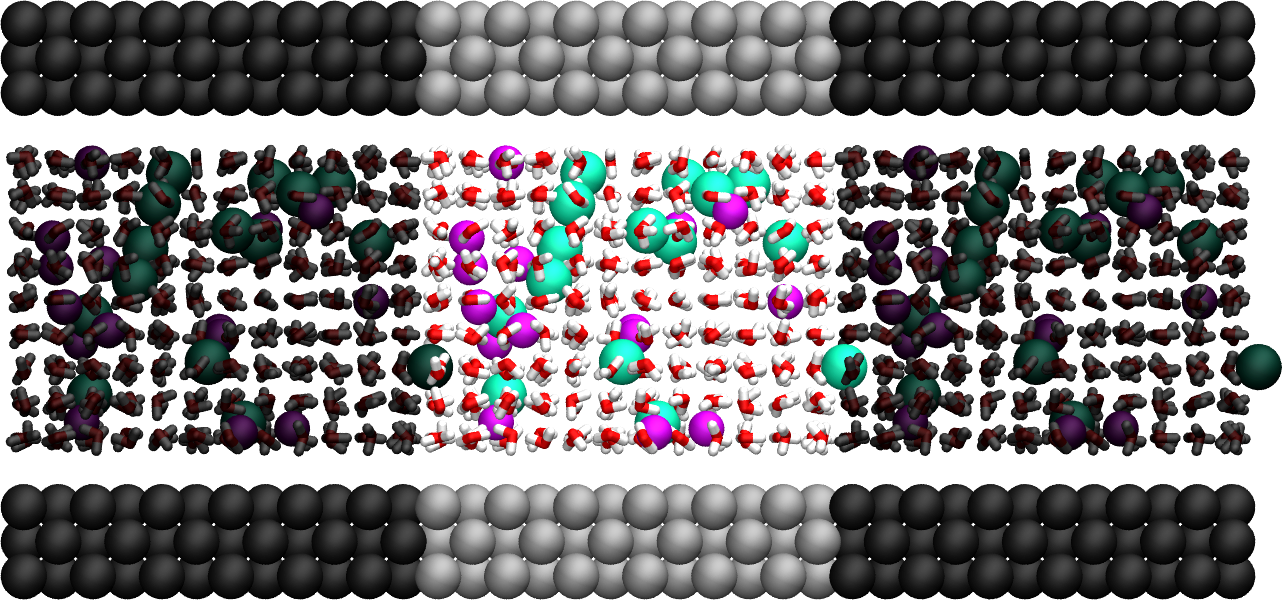
\includegraphics[width=\linewidth]{NANOSHEAR-system}
\caption{Side view of the system. Periodic images are represented in darker colors.
Water molecules are in red and white, $\text{Na}^+$ ions in purple, $\text{Cl}^-$
ions in lime, and wall atoms in gray. Note the absence of atomic defect at the
cell boundaries.}
\label{fig:NANOSHEAR-system}
\end{figure}

\paragraph{Energy minimization}
Let us move the atoms and place them in more energetically favorable positions
before starting the actual molecular dynamics simulation. Let us call this step
\textit{energy minimization}, although it is not a conventional \textit{minimization}
as done for instance in the first tutorial; \hyperref[lennard-jones-label]{Lennard-Jones fluid}.
Instead, a molecular dynamics simulation will be performed here, with some techniques
employed to prevent the system from exploding due to overlapping atoms.

Let us create a new folder called \flrcmd{minimization/} next to \flrcmd{systemcreation/},
and create a new input file called \flecmd{input.lmp} in it. Copy the following lines
in \flecmd{input.lmp}:
\begin{lstlisting}
boundary p p f
units real
atom_style full
bond_style harmonic
angle_style harmonic
pair_style lj/cut/tip4p/long O H O-H H-O-H &
    0.1546 12.0
kspace_style pppm/tip4p 1.0e-4
kspace_modify slab 3.0

read_data ../systemcreation/system.data

include ../PARM.lmp
include ../GROUP.lmp
\end{lstlisting}
The only difference from the previous input is that instead of creating a new
box and new atoms, we open the previously created file \flecmd{system.data}
located in \flrcmd{systemcreation/}. The file \flecmd{system.data} contains the
definition of the simulation box and the positions of the atoms.

Now, let us create a first simulation step using a relatively small
timestep ($0.5\,\text{fs}$) and a low temperature of $T = 1\,\text{K}$:
\begin{lstlisting}
fix mynve fluid nve/limit 0.1
fix myber fluid temp/berendsen 1 1 100
fix myshk H2O shake 1.0e-4 200 0 b O-H a H-O-H
timestep 0.5
\end{lstlisting}
Just like \textit{fix nve}, the \textit{fix nve/limit} command performs constant
NVE integration to update the positions and velocities of the atoms at each
timestep. The difference is that \textit{fix nve/limit} also limits the maximum
distance atoms can travel at each timestep. Here, the chosen maximum distance
is $0.1~\text{\AA{}}$. Because the \textit{fix nve/limit} is applied to the
group \textit{fluid}, only the water molecules and ions will move.
The \textit{fix temp/berendsen} rescales the velocities of the atoms to
force the temperature of the system to reach the desired value of $1~\text{K}$,
and the SHAKE algorithm is used in order to maintain the shape of the water molecules.

Let us also create images of the system and control
the printing of thermodynamic outputs by adding the following lines to \flecmd{input.lmp}:
\begin{lstlisting}
dump mydmp all image 200 dump.*.jpg type type &
    shiny 0.1 box no 0.01 view 90 0 zoom 1.8
dump_modify mydmp backcolor white &
    acolor O red adiam O 2 &
    acolor H white adiam H 1 &
    acolor Na+ blue adiam Na+ 2.5 &
    acolor Cl- cyan adiam Cl- 3 &
    acolor WALL gray adiam WALL 3
thermo 200
\end{lstlisting}
Finally, let us run for 4000 steps. Add the following lines into \flecmd{input.lmp}:
\begin{lstlisting}
run 4000
\end{lstlisting}
When running the \flecmd{input.lmp} file with LAMMPS, you should see that the
total energy of the system is initially very high, but rapidly decreases and
reach a plateau (Fig.\,\ref{fig:NANOSHEAR-minimization}). From the generated image of the system,
you will see that some of the atoms are moving, particularly those that were
initially in problematic positions.

In order to better equilibrate the system, let us perform two additional steps
with a larger timestep and a higher imposed temperature:
\begin{lstlisting}
fix myber fluid temp/berendsen 300 300 100
timestep 1.0

run 4000

unfix mynve
fix mynve fluid nve

run 4000

write_data system.data nocoeff
\end{lstlisting}
For the last of the three steps, fix \textit{nve} is used instead of
\textit{nve/limit}, which will allow for better relaxation of the atom positions.

When running the \flecmd{input.lmp} file with LAMMPS, you should see that the
the temperature reaches the desired value of $300\,\text{K}$. The generated file
\flecmd{system.data} contains the final state of the system.

\begin{figure}
\centering
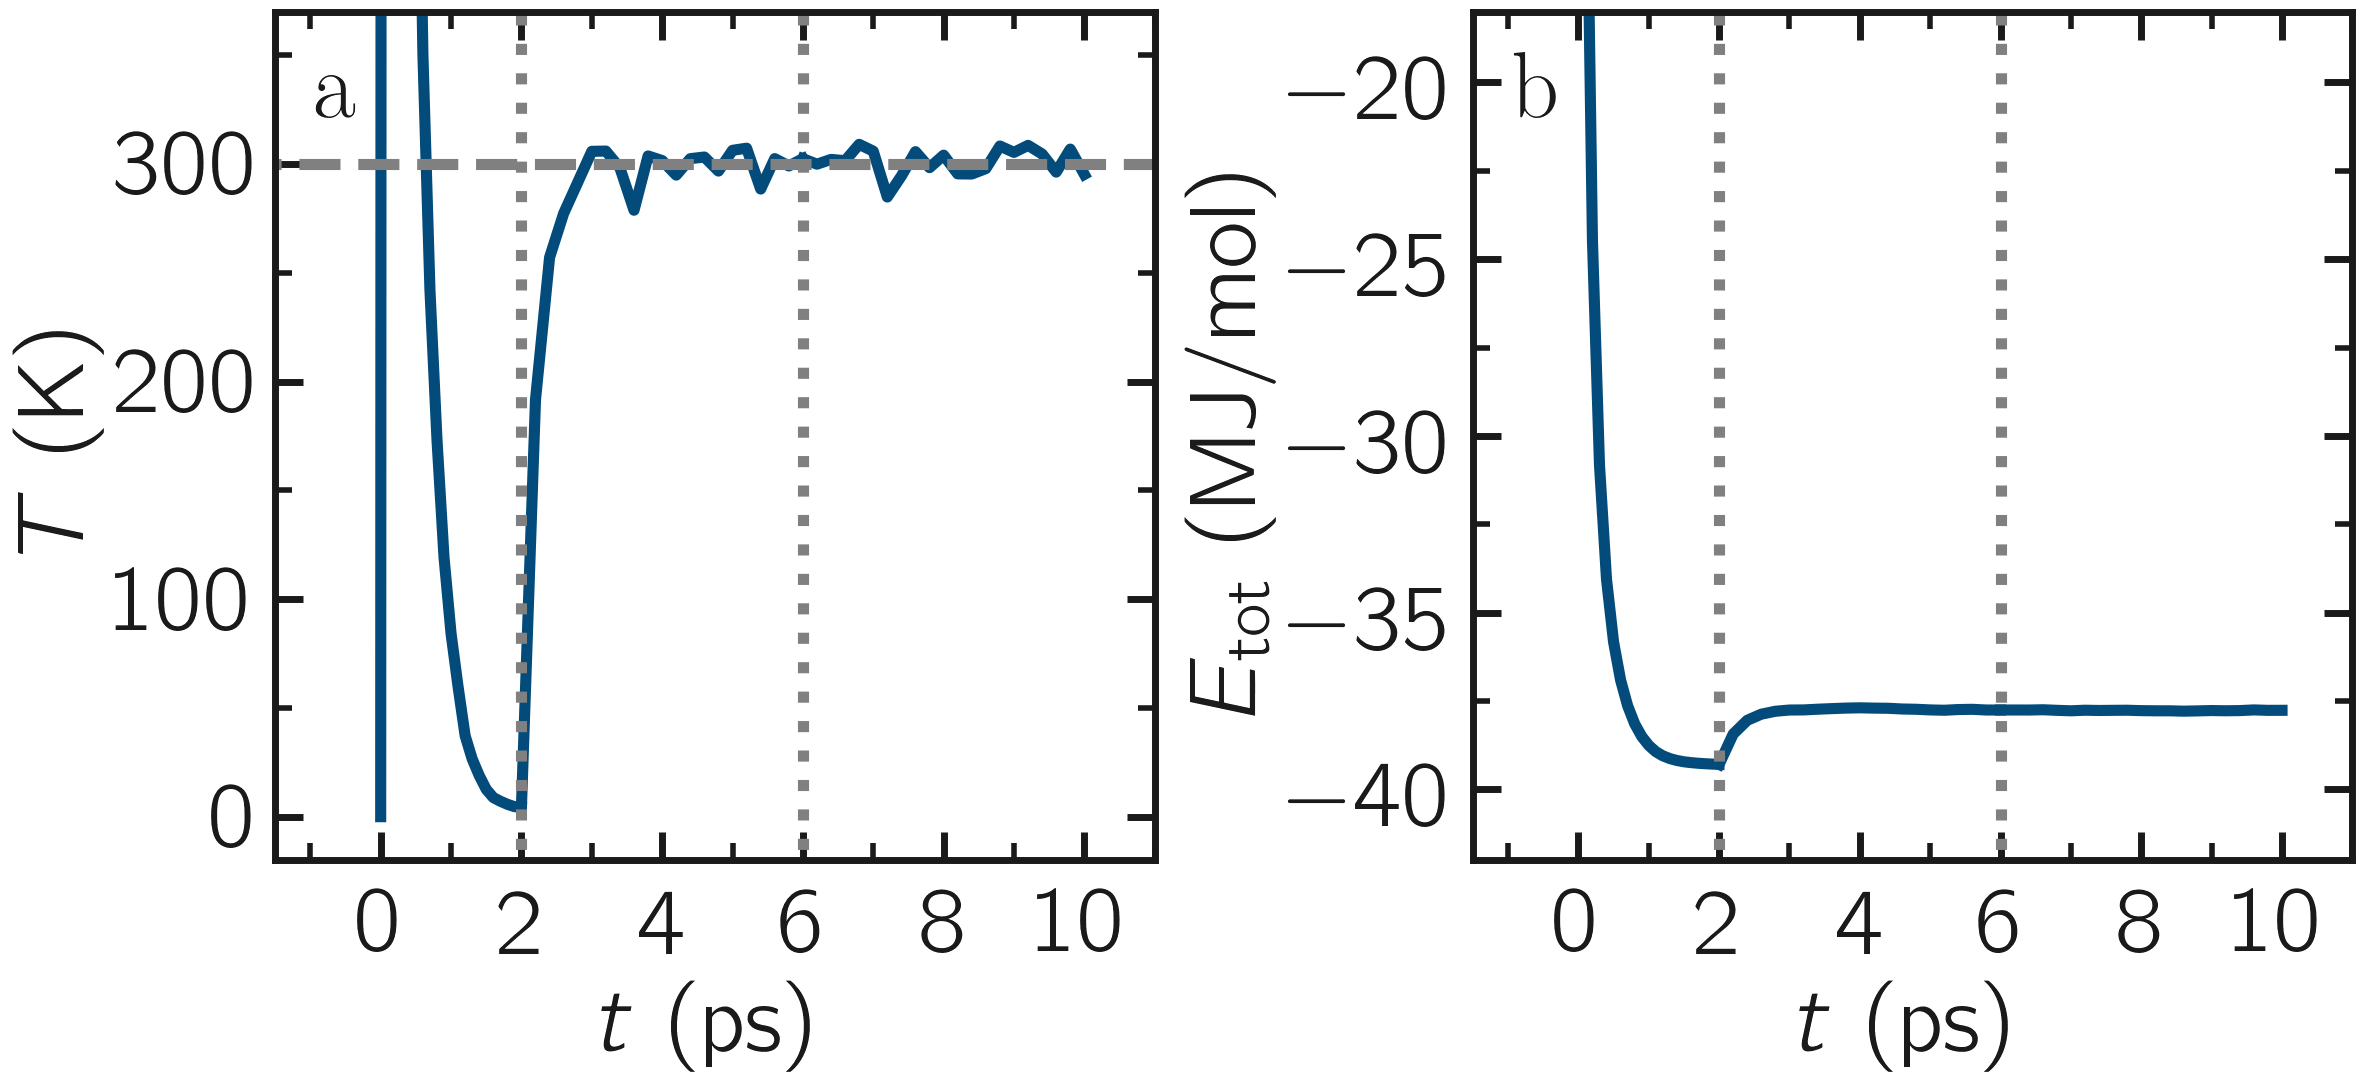
\includegraphics[width=\linewidth]{NANOSHEAR-minimization}
\caption{Total energy of the system $E_\text{tot}$ as a function of time $t$
extracted from the log file using \textit{Python} and \textit{lammps\_logfile}
\cite{sveinsson2021logfile}. The vertical dashed lines demarcate the three
consecutive steps.}
\label{fig:NANOSHEAR-minimization}
\end{figure}

\paragraph{System equilibration}
Let us equilibrate further the entire system by letting both fluid and piston
relax at ambient temperature. Create a new folder called \flrcmd{equilibration/}
next to the previously created folders, and create a new \flecmd{input.lmp}
file in it. Add the following lines into \flecmd{input.lmp}:
\begin{lstlisting}
boundary p p f
units real
atom_style full
bond_style harmonic
angle_style harmonic
pair_style lj/cut/tip4p/long O H O-H H-O-H &
    0.1546 12.0
kspace_style pppm/tip4p 1.0e-4
kspace_modify slab 3.0

read_data ../minimization/system.data

include ../PARM.lmp
include ../GROUP.lmp

fix mynve all nve
fix myber all temp/berendsen 300 300 100
fix myshk H2O shake 1.0e-4 200 0 b O-H a H-O-H
fix myrct all recenter NULL NULL 0
timestep 1.0
\end{lstlisting}
The fix \textit{recenter} does not influence the dynamics but will keep the
system in the center of the box, which makes the
visualization easier. Then, add the following lines into \flecmd{input.lmp}
for the trajectory visualization and output:
\begin{lstlisting}

dump mydmp all image 200 dump.*.jpg type type &
    shiny 0.1 box no 0.01 view 90 0 zoom 1.8
dump_modify mydmp backcolor white &
    acolor O red adiam O 2 &
    acolor H white adiam H 1 &
    acolor Na+ blue adiam Na+ 2.5 &
    acolor Cl- cyan adiam Cl- 3 &
    acolor WALL gray adiam WALL 3
thermo 500
variable walltopz equal xcm(walltop,z)
variable wallbotz equal xcm(wallbot,z)
variable deltaz equal v_walltopz-v_wallbotz
fix myat1 all ave/time 100 1 100 v_deltaz &
    file interwall_distance.dat
\end{lstlisting}
The first two variables extract the centers of mass of the two walls. Then,
the \textit{deltaz} variable is used to calculate the distance between the two
variables \textit{walltopz} and \textit{wallbotz}, i.e.~the distance between the two walls.

Finally, let us add the \textit{run} command:
\begin{lstlisting}
run 30000
write_data system.data nocoeff
\end{lstlisting}
Run the \flecmd{input.lmp} file using LAMMPS. As seen from the data printed by
\textit{fix myat1}, the distance between the two walls reduces until it reaches
an equilibrium value (Fig.\,\ref{fig:NANOSHEAR-equilibration}).

Note that it is generally recommended to run longer equilibration. Here, for
instance, the slowest process in the system is probably the ionic diffusion.
Therefore, the equilibration should in principle be longer than the time
the ions need to diffuse over the size of the pore ($\approx 1.2\,\text{nm}$),
i.e.~on the order of half a nanosecond.

\begin{figure}
\centering
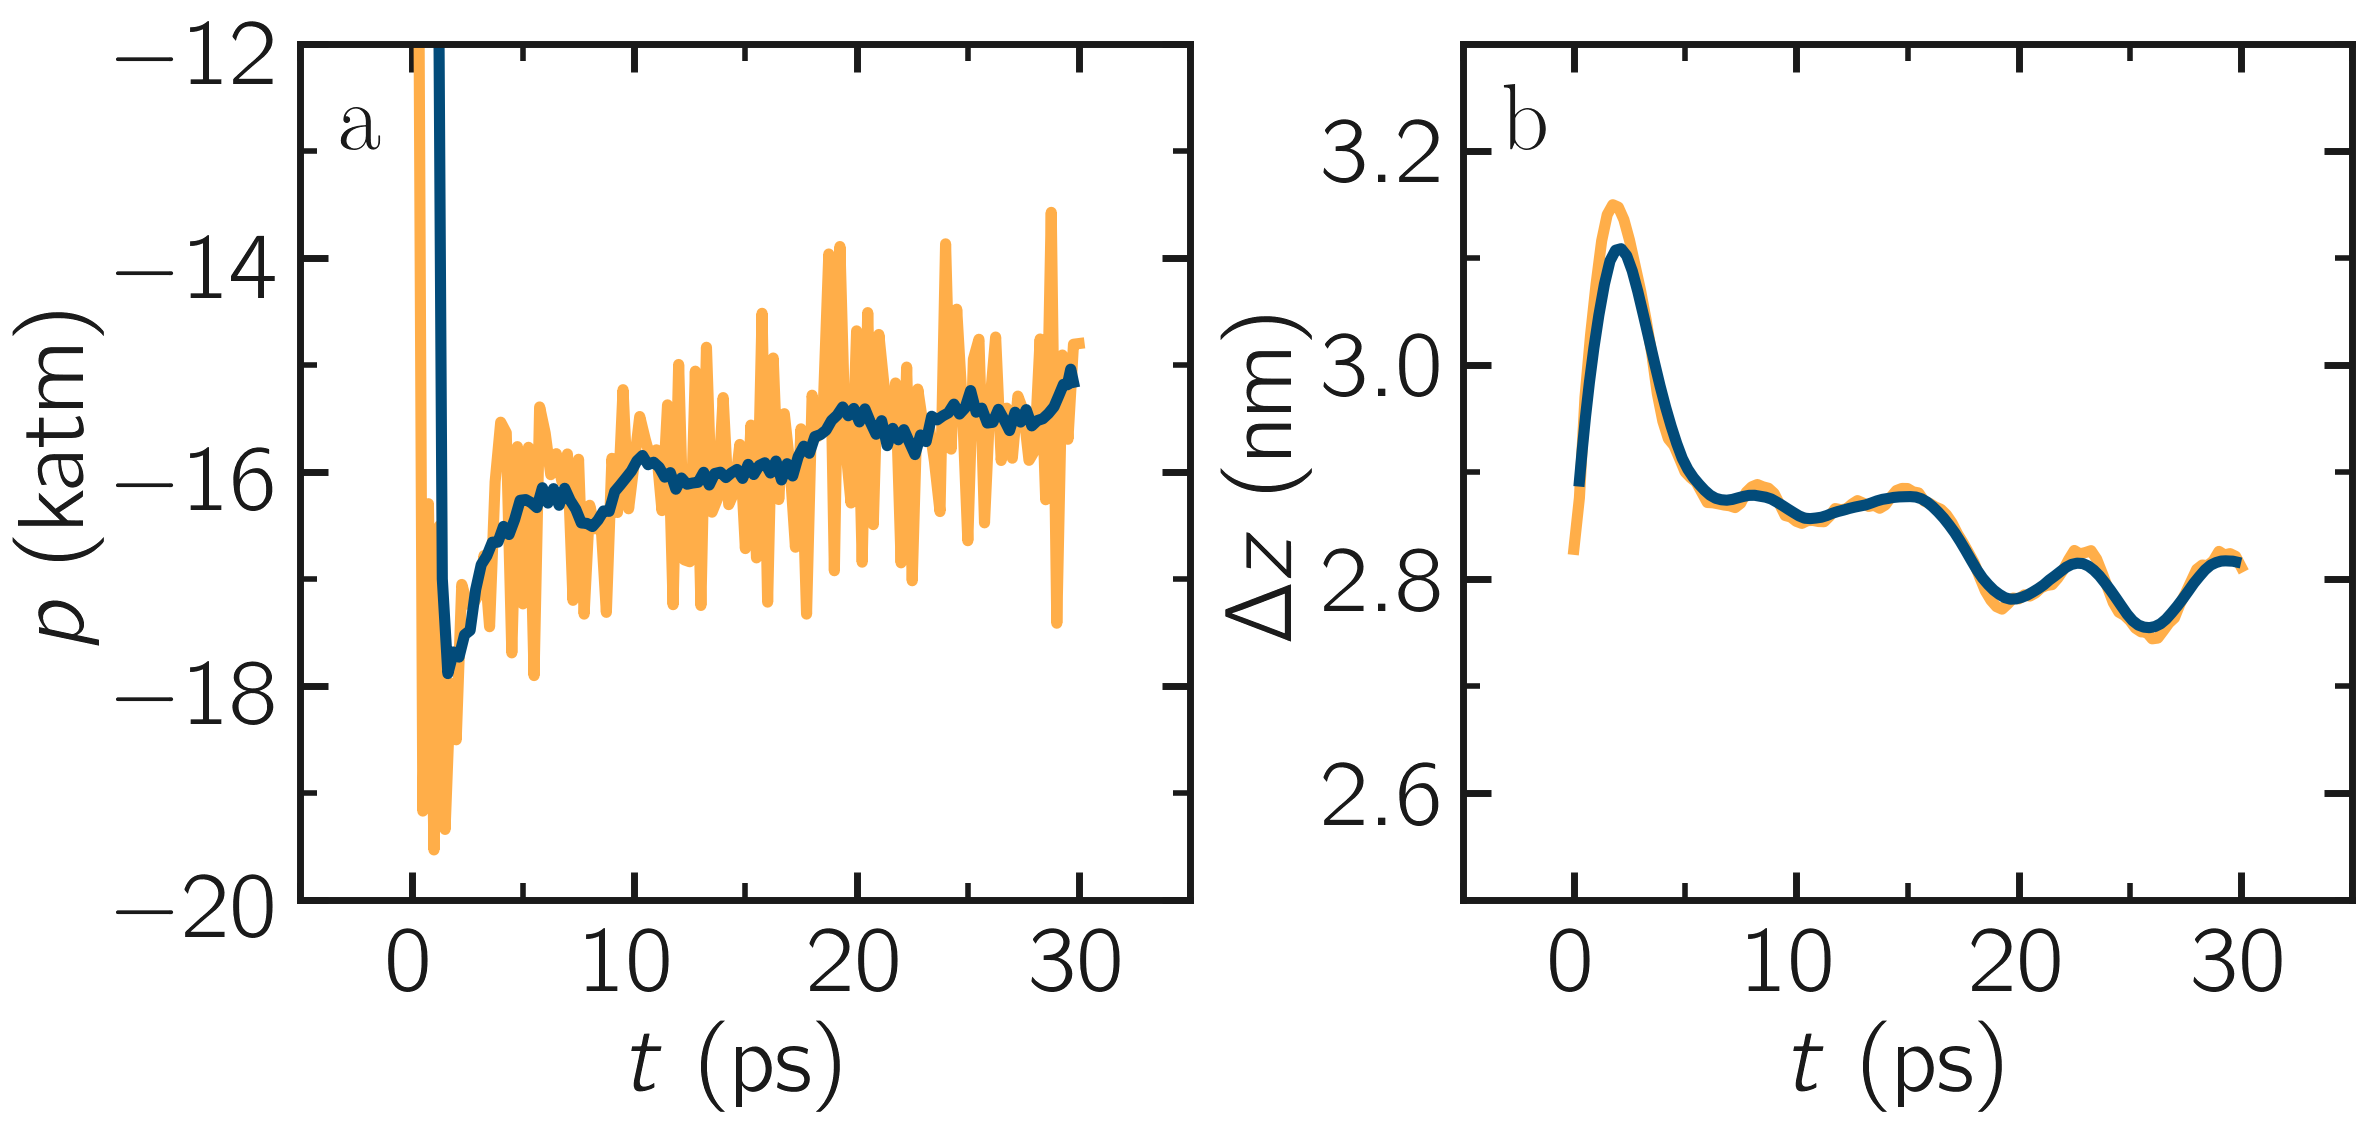
\includegraphics[width=\linewidth]{NANOSHEAR-equilibration}
\caption{Distance between the walls $d$ as a function of time $t$.}
\label{fig:NANOSHEAR-equilibration}
\end{figure}

\subsubsection{Imposed shearing}

From the equilibrated configuration, let us impose a lateral motion on the two
walls and shear the electrolyte. In a new folder called \flrcmd{shearing/},
create a new \flecmd{input.lmp} file that starts like the previous ones:
\begin{lstlisting}
boundary p p f
units real
atom_style full
bond_style harmonic
angle_style harmonic
pair_style lj/cut/tip4p/long O H O-H H-O-H &
    0.1546 12.0
kspace_style pppm/tip4p 1.0e-4
kspace_modify slab 3.0
\end{lstlisting}
Let us import the previously equilibrated data, include the parameter and group
files, and then deal with the dynamics of the system.
\begin{lstlisting}
read_data ../equilibration/system.data

include ../PARM.lmp
include ../GROUP.lmp

fix mynve all nve
compute Tfluid fluid temp/partial 0 1 1
fix myber1 fluid temp/berendsen 300 300 100
fix_modify myber1 temp Tfluid
compute Twall wall temp/partial 0 1 1
fix myber2 wall temp/berendsen 300 300 100
fix_modify myber2 temp Twall
fix myshk H2O shake 1.0e-4 200 0 b O-H a H-O-H
fix myrct all recenter NULL NULL 0
\end{lstlisting}
One difference with the previous input is that, here, two thermostats are used,
one for the fluid (\textit{myber1}) and one for the solid (\textit{myber2}).
The use of \textit{fix\_modify} together with \textit{compute temp} ensures
that the right temperature value is used by the thermostats. The use of
temperature \textit{compute} with \textit{temp/partial 0 1 1} is meant to exclude
the \textit{x} coordinate from the thermalization, which is important since a
large velocity will be imposed along \textit{x}.

Then, let us impose the velocity of the two walls by adding the following
commands to \flecmd{input.lmp}:
\begin{lstlisting}
fix mysf1 walltop setforce 0 NULL NULL
fix mysf2 wallbot setforce 0 NULL NULL
velocity wallbot set -2e-4 NULL NULL
velocity walltop set 2e-4 NULL NULL
\end{lstlisting}
The \textit{setforce} commands cancel the forces on \textit{walltop} and
\textit{wallbot}, respectively. Therefore the atoms of the two groups do not
experience any force from the rest of the system. In the absence of force acting
on those atoms, they will conserve their initial velocity. The \textit{velocity}
commands act only once and impose the velocity of the atoms of the groups
\textit{wallbot} and \textit{walltop}, respectively.

Finally, let us dump the atom positions, and extract the velocity profiles using
several \textit{ave/chunk} commands, extract the force applied on the walls, and
then run for $200\,\text{ps}$ Add the following lines into \flecmd{input.lmp}:
\begin{lstlisting}
dump mydmp all image 200 dump.*.jpg type type &
    shiny 0.1 box no 0.01 view 90 0 zoom 1.8
dump_modify mydmp backcolor white &
    acolor O red adiam O 2 &
    acolor H white adiam H 1 &
    acolor Na+ blue adiam Na+ 2.5 &
    acolor Cl- cyan adiam Cl- 3 &
    acolor WALL gray adiam WALL 3

thermo 500
thermo_modify temp Tfluid

compute cc1 H2O chunk/atom bin/1d z 0.0 1.0
compute cc2 wall chunk/atom bin/1d z 0.0 1.0
compute cc3 ions chunk/atom bin/1d z 0.0 1.0

fix myac1 H2O ave/chunk 10 15000 200000 &
cc1 density/mass vx file water.profile_1A.dat
fix myac2 wall ave/chunk 10 15000 200000 &
cc2 density/mass vx file wall.profile_1A.dat
fix myac3 ions ave/chunk 10 15000 200000 &
cc3 density/mass vx file ions.profile_1A.dat

fix myat1 all ave/time 10 100 1000 f_mysf1[1] &
    f_mysf2[1] file forces.dat

timestep 1.0
run 200000
write_data system.data nocoeff
\end{lstlisting}
Here, a binning of $1\,\text{\AA{}}$ is used for the density profiles generated
by the \textit{ave/chunk} commands. For smoother profiles, you can reduce the value
of the bins. The averaged velocity and density profiles of the fluid are plotted
in Figs.\ref{fig:NANOSHEAR-velocity}-\ref{fig:NANOSHEAR-density}. As expected for
such Couette flow geometry, the velocity of the fluid is found to increase linearly
along $z$.

\begin{figure}
\centering
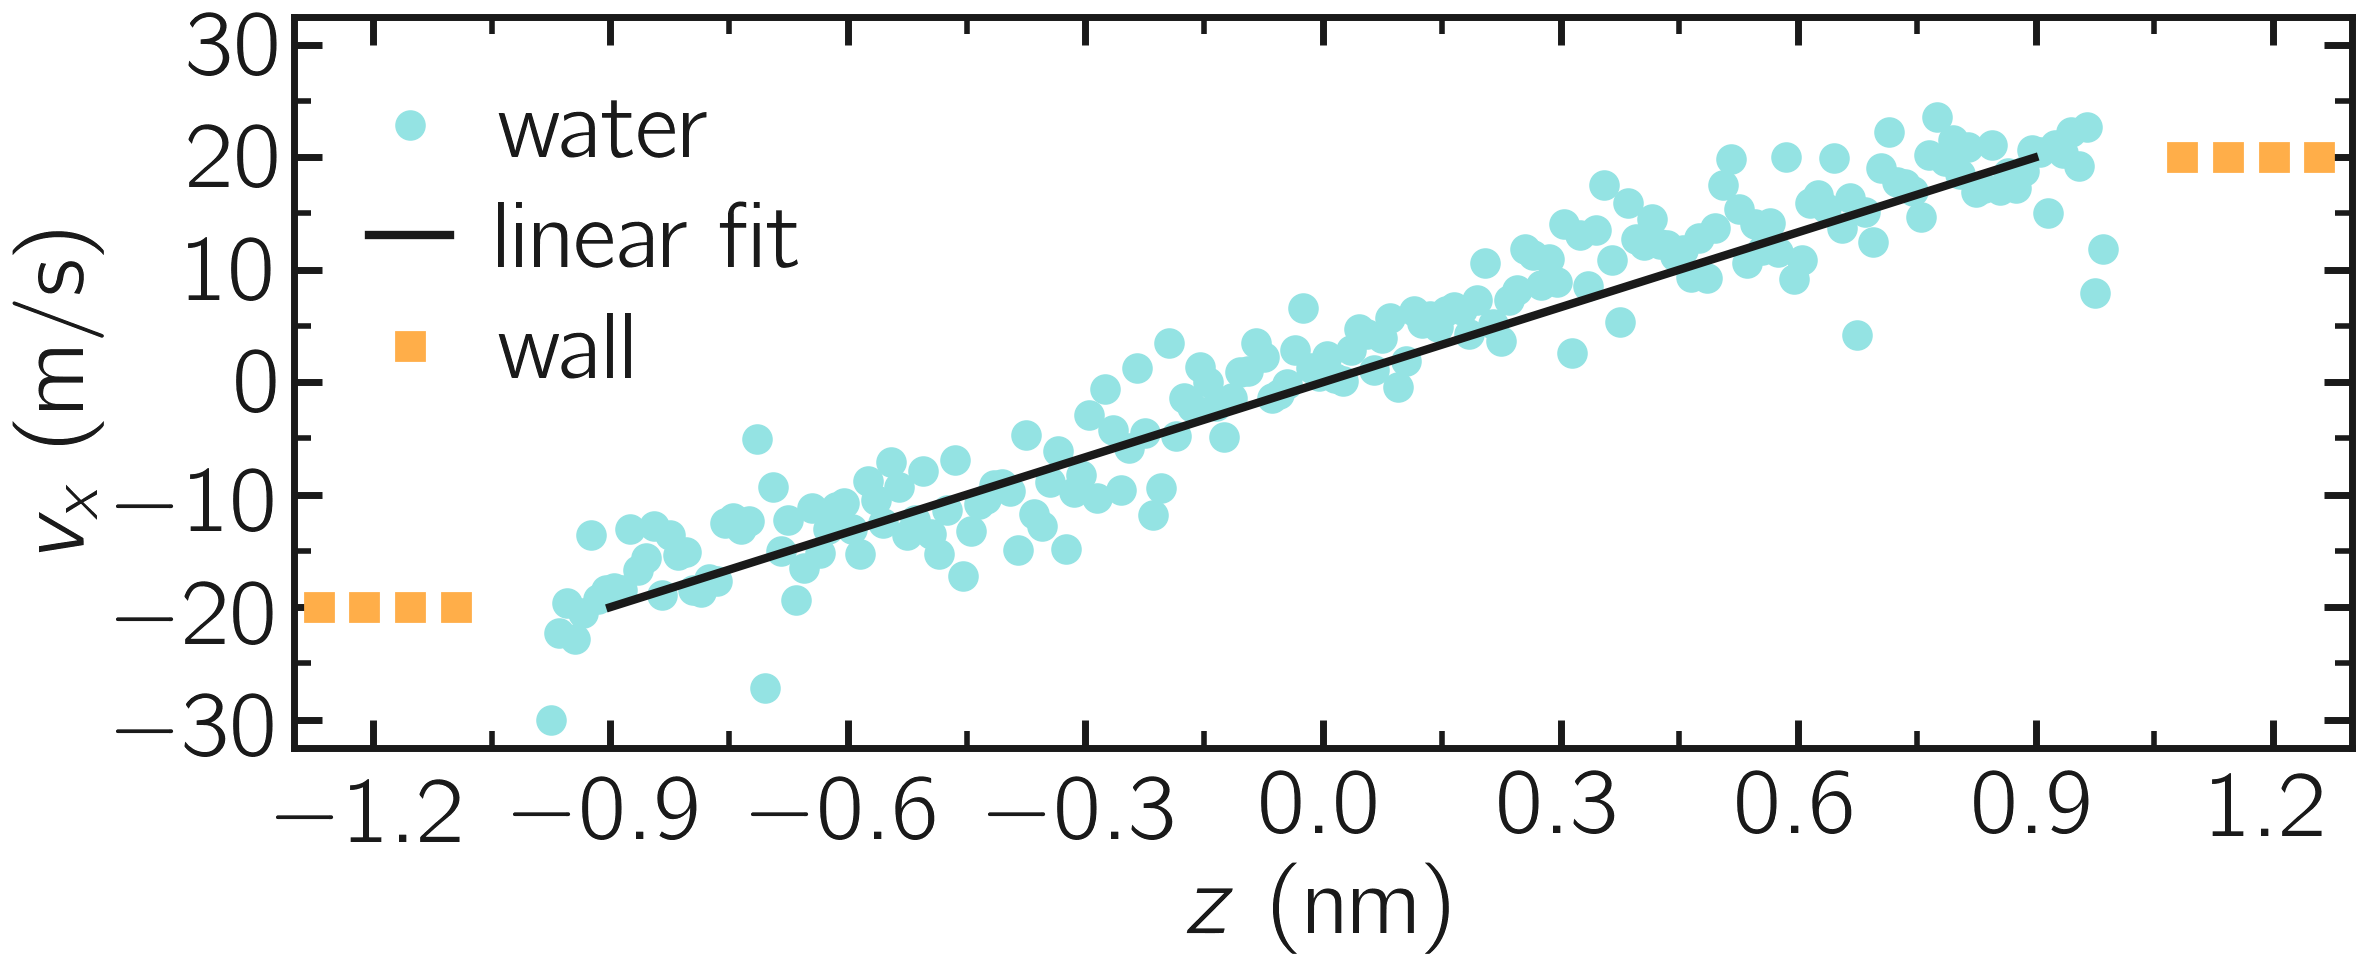
\includegraphics[width=\linewidth]{NANOSHEAR-velocity}
\caption{Velocity profiles for water molecules and ions (blue disks), and walls
(orange squares) along the \textit{z} axis. The line is a linear fit assuming
that the pore size is $h = 1.8\,\text{nm}$.}
\label{fig:NANOSHEAR-velocity}
\end{figure}

\begin{figure}
\centering
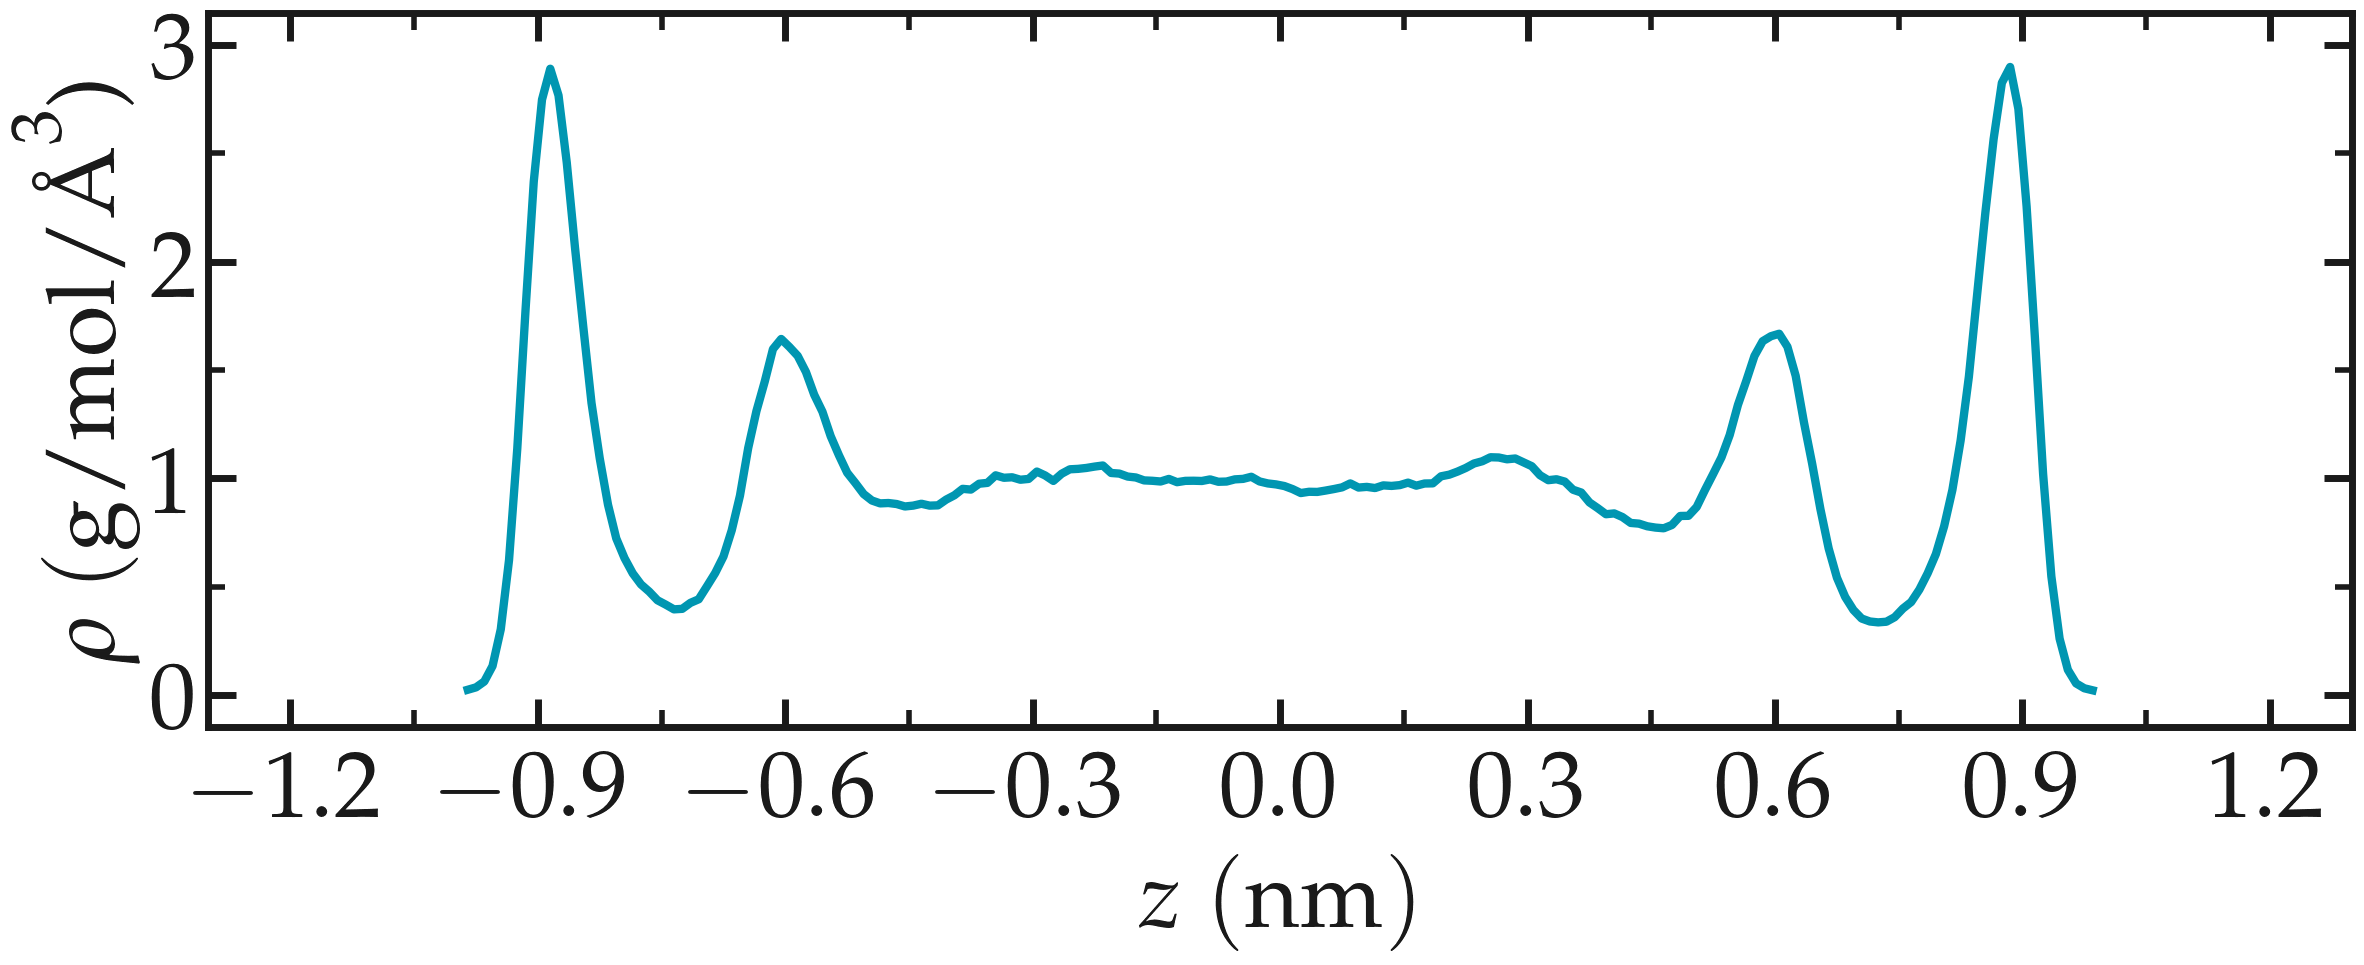
\includegraphics[width=\linewidth]{NANOSHEAR-density}
\caption{Water density $\rho$ along the \textit{z} axis.}
\label{fig:NANOSHEAR-density}
\end{figure}

From the force applied by the fluid on the solid, one can extract the stress
within the fluid, which allows for the measurement of its viscosity $\dot{\eta}$
according to $\eta = \tau / \dot{\gamma}$ where $\tau$ is the stress applied by
the fluid on the shearing wall, and $\dot{\gamma}$ the shear rate (which is
imposed here) \cite{gravelle2021violations}. Here, the shear rate is
approximatively $\dot{\gamma} = 16 \cdot 10^9\,\text{s}^{-1}$, and using a
surface area of $A = 6 \cdot 10^{-18}\,\text{m}^2$, one gets an estimate for
the shear viscosity for the confined fluid of $\eta = 6.6\,\text{mPa.s}$. The
viscosity calculated at such a high shear rate may differ from the expected
\textit{bulk} value. In general, it is recommended to use a lower value for the
shear rate. Note that for lower shear rates, the ratio of noise-to-signal is
larger, and longer simulations are needed. Another important point to keep in
mind is that the viscosity of a fluid next to a solid surface is typically larger
than in bulk due to interaction with the walls \cite{wolde-kidanInterplayInterfacialViscosity2021}.
Therefore, one expects the present simulation to return a viscosity that is slightly
larger than what would be measured in the absence of a wall.

\subsection{Tutorial 5: Reactive silicon dioxide}
\label{reactive-silicon-dioxide-label}

\begin{figure}
\centering
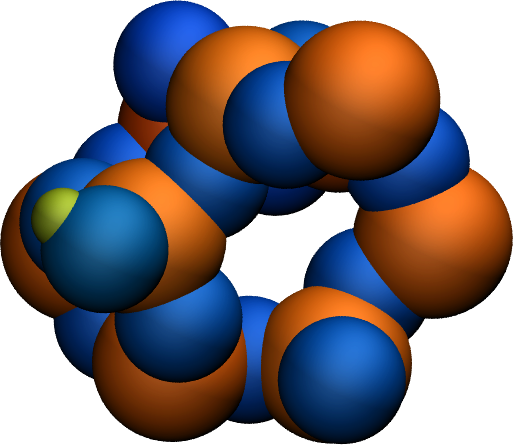
\includegraphics[width=0.55\linewidth]{SIO}
\caption{A portion of the silicon dioxide structure as simulated during
\hyperref[reactive-silicon-dioxide-label]{Tutorial 5}. Atoms are colored by their charges.}
\label{fig:SIO}
\end{figure}

\noindent The objective of this tutorial is to use the reactive force field ReaxFF
to calculate the partial charges of a system undergoing deformation, as well as
the formation and breaking of chemical bonds \cite{van2001reaxff, zou2012investigation}.
The system simulated here is a block of silicon dioxide $\text{SiO}_2$ (Fig.\,\ref{fig:SIO})
that is deformed until rupture. Particular attention is given to the evolution of
the atomic charges during the deformation of the structure, and the chemical
reactions occurring due to the deformation are tracked over time.

\subsubsection{Prepare and relax}
Create a folder, name it \flrcmd{RelaxSilica/}, and download the initial topology
of a small amorphous silica structure called
\href{\filepath tutorial5/silica.data}{\dwlcmd{silica.data}}.
This structure was created using a classical force field called
Vashishta \cite{vashishta1990interaction}. If you open the \flecmd{silica.data}
file, you will see in the Atoms section that all silicon atoms have the same
charge $q = 1.1\,\text{e}$, and all oxygen atoms have the charge $q = -0.55\,\text{e}$.
This is common with classical force fields and will change once ReaxFF is used.

The first action we need to perform here is to relax the structure with ReaxFF,
which we are gonna do using molecular dynamics. To make sure that the system
equilibrates nicely, let us track some parameters over time. Create an input
file called \flecmd{input.lmp} in \flrcmd{RelaxSilica/}, and copy the following
lines into it:
\begin{lstlisting}
units real
atom_style full

read_data silica.data

mass Si 28.0855
mass O 15.999
\end{lstlisting}
So far, the input is very similar to what was seen in the previous tutorials.
Some basic parameters are defined (\textit{units}, \textit{atom\_style} and \textit{masses}),
and the \flecmd{.data} file is imported by the \textit{read\_data} command.

Now, let us copy three crucial lines into the \flecmd{input.lmp} file:
\begin{lstlisting}
pair_style reaxff NULL safezone 3.0 mincap 150
pair_coeff * * reaxCHOFe.ff Si O
fix myqeq all qeq/reaxff 1 0.0 10.0 1.0e-6 &
    reaxff maxiter 400
\end{lstlisting}
Here, the \textit{pair\_style reaxff} is used with no control file. The
\textit{safezone} and \textit{mincap} keywords have been added to avoid memory
allocation issues, which sometimes can trigger the segmentation faults and
\textit{bondchk} failed errors. The \textit{pair\_coeff} uses the
\href{\filepath tutorial5/reaxCHOFe.ff}{\dwlcmd{reaxCHOFe.ff}}
file, which must be downloaded and saved within \flrcmd{RelaxSilica/}. Finally, the
\textit{fix qeq/reaxff} is used to perform charge equilibration \cite{rappe1991charge}.
The charge equilibration occurs at every step. The values 0.0 and 10.0 are the
low and the high cutoffs, respectively, and $1.0 \text{e} -6$ is a tolerance.
Finally, \textit{maxiter} sets an upper limit to the number of attempts to
equilibrate the charge.

Then, let us add some commands to the \flecmd{input.lmp} file  to measure the
evolution of the charges during the simulation:
\begin{lstlisting}
group grpSi type Si
group grpO type O
variable qSi equal charge(grpSi)/count(grpSi)
variable qO equal charge(grpO)/count(grpO)
\end{lstlisting}
Let us also print the charge in the \textit{.log} file by using \textit{thermo\_style},
and create images of the system. Add the following lines into the \flecmd{input.lmp}:
\begin{lstlisting}
thermo 200
thermo_style custom step temp etotal press &
    vol v_qSi v_qO
dump mydmp all image 200 dump.*.jpg type type &
    shiny 0.1 box no 0.01 view 0 0 zoom 1.8
dump_modify mydmp backcolor white &
    acolor Si yellow adiam Si 2.5 &
    acolor O red adiam O 2
\end{lstlisting}

In order to also visualize the system using an external tool, VMD, let us also
create a \textit{.lammpstrj} file for visualization:
\begin{lstlisting}
dump dmp all custom 200 dump.lammpstrj &
    id typelabel q x y z
\end{lstlisting}
The \textit{.lammpstrj} that will be created when running lammps will contain
6 columns with respectively the atom IDs, the atom types, the atom charges ($q$),
and finally the atom coordinates ($x$, $y$, and $z$).

Let us also use the \textit{fix reaxff/species} to evaluate what species are
present within the simulation. It will be useful later when the system is deformed
and some bonds are broken:
\begin{lstlisting}
fix myspec all reaxff/species 5 1 5 &
    species.log element Si O
\end{lstlisting}
Here, the information will be printed every 5 steps in a file called \textit{species.log}.
Let us perform a very short run using the anisotropic NPT command and relax the
density of the system.
\begin{lstlisting}
velocity all create 300.0 3482028
fix mynpt all npt temp 300.0 300.0 100 &
    aniso 1.0 1.0 1000
timestep 0.5

run 5000

write_data silica-relaxed.data
\end{lstlisting}
Run the \flecmd{input.lmp} file using LAMMPS. As seen from \textit{species.log},
only one species is detected, called O384Si192, representing the entire system.
The value of the charge of the atoms can be extracted from the \textit{dump.lammpstrj}
file using Python. You can use this
\href{\filepath tutorial5/dump-reader.py}{\dwlcmd{dump-reader.py}}
script to import the charge values into Python.
As the simulation progresses, the charge of every atom fluctuates
because it is adjusting to the local environment of the atom (Fig.\,\ref{fig:SIO-charge}).
It can also be seen that the averaged charges for both silicon and oxygen
atoms vary abruptly at the beginning of the simulation, which correlates with
a rapid volume change of the box during which the inter-atomic distances are
expected to quickly change (Fig.\,\ref{fig:SIO-volume}).

\begin{figure}
\centering
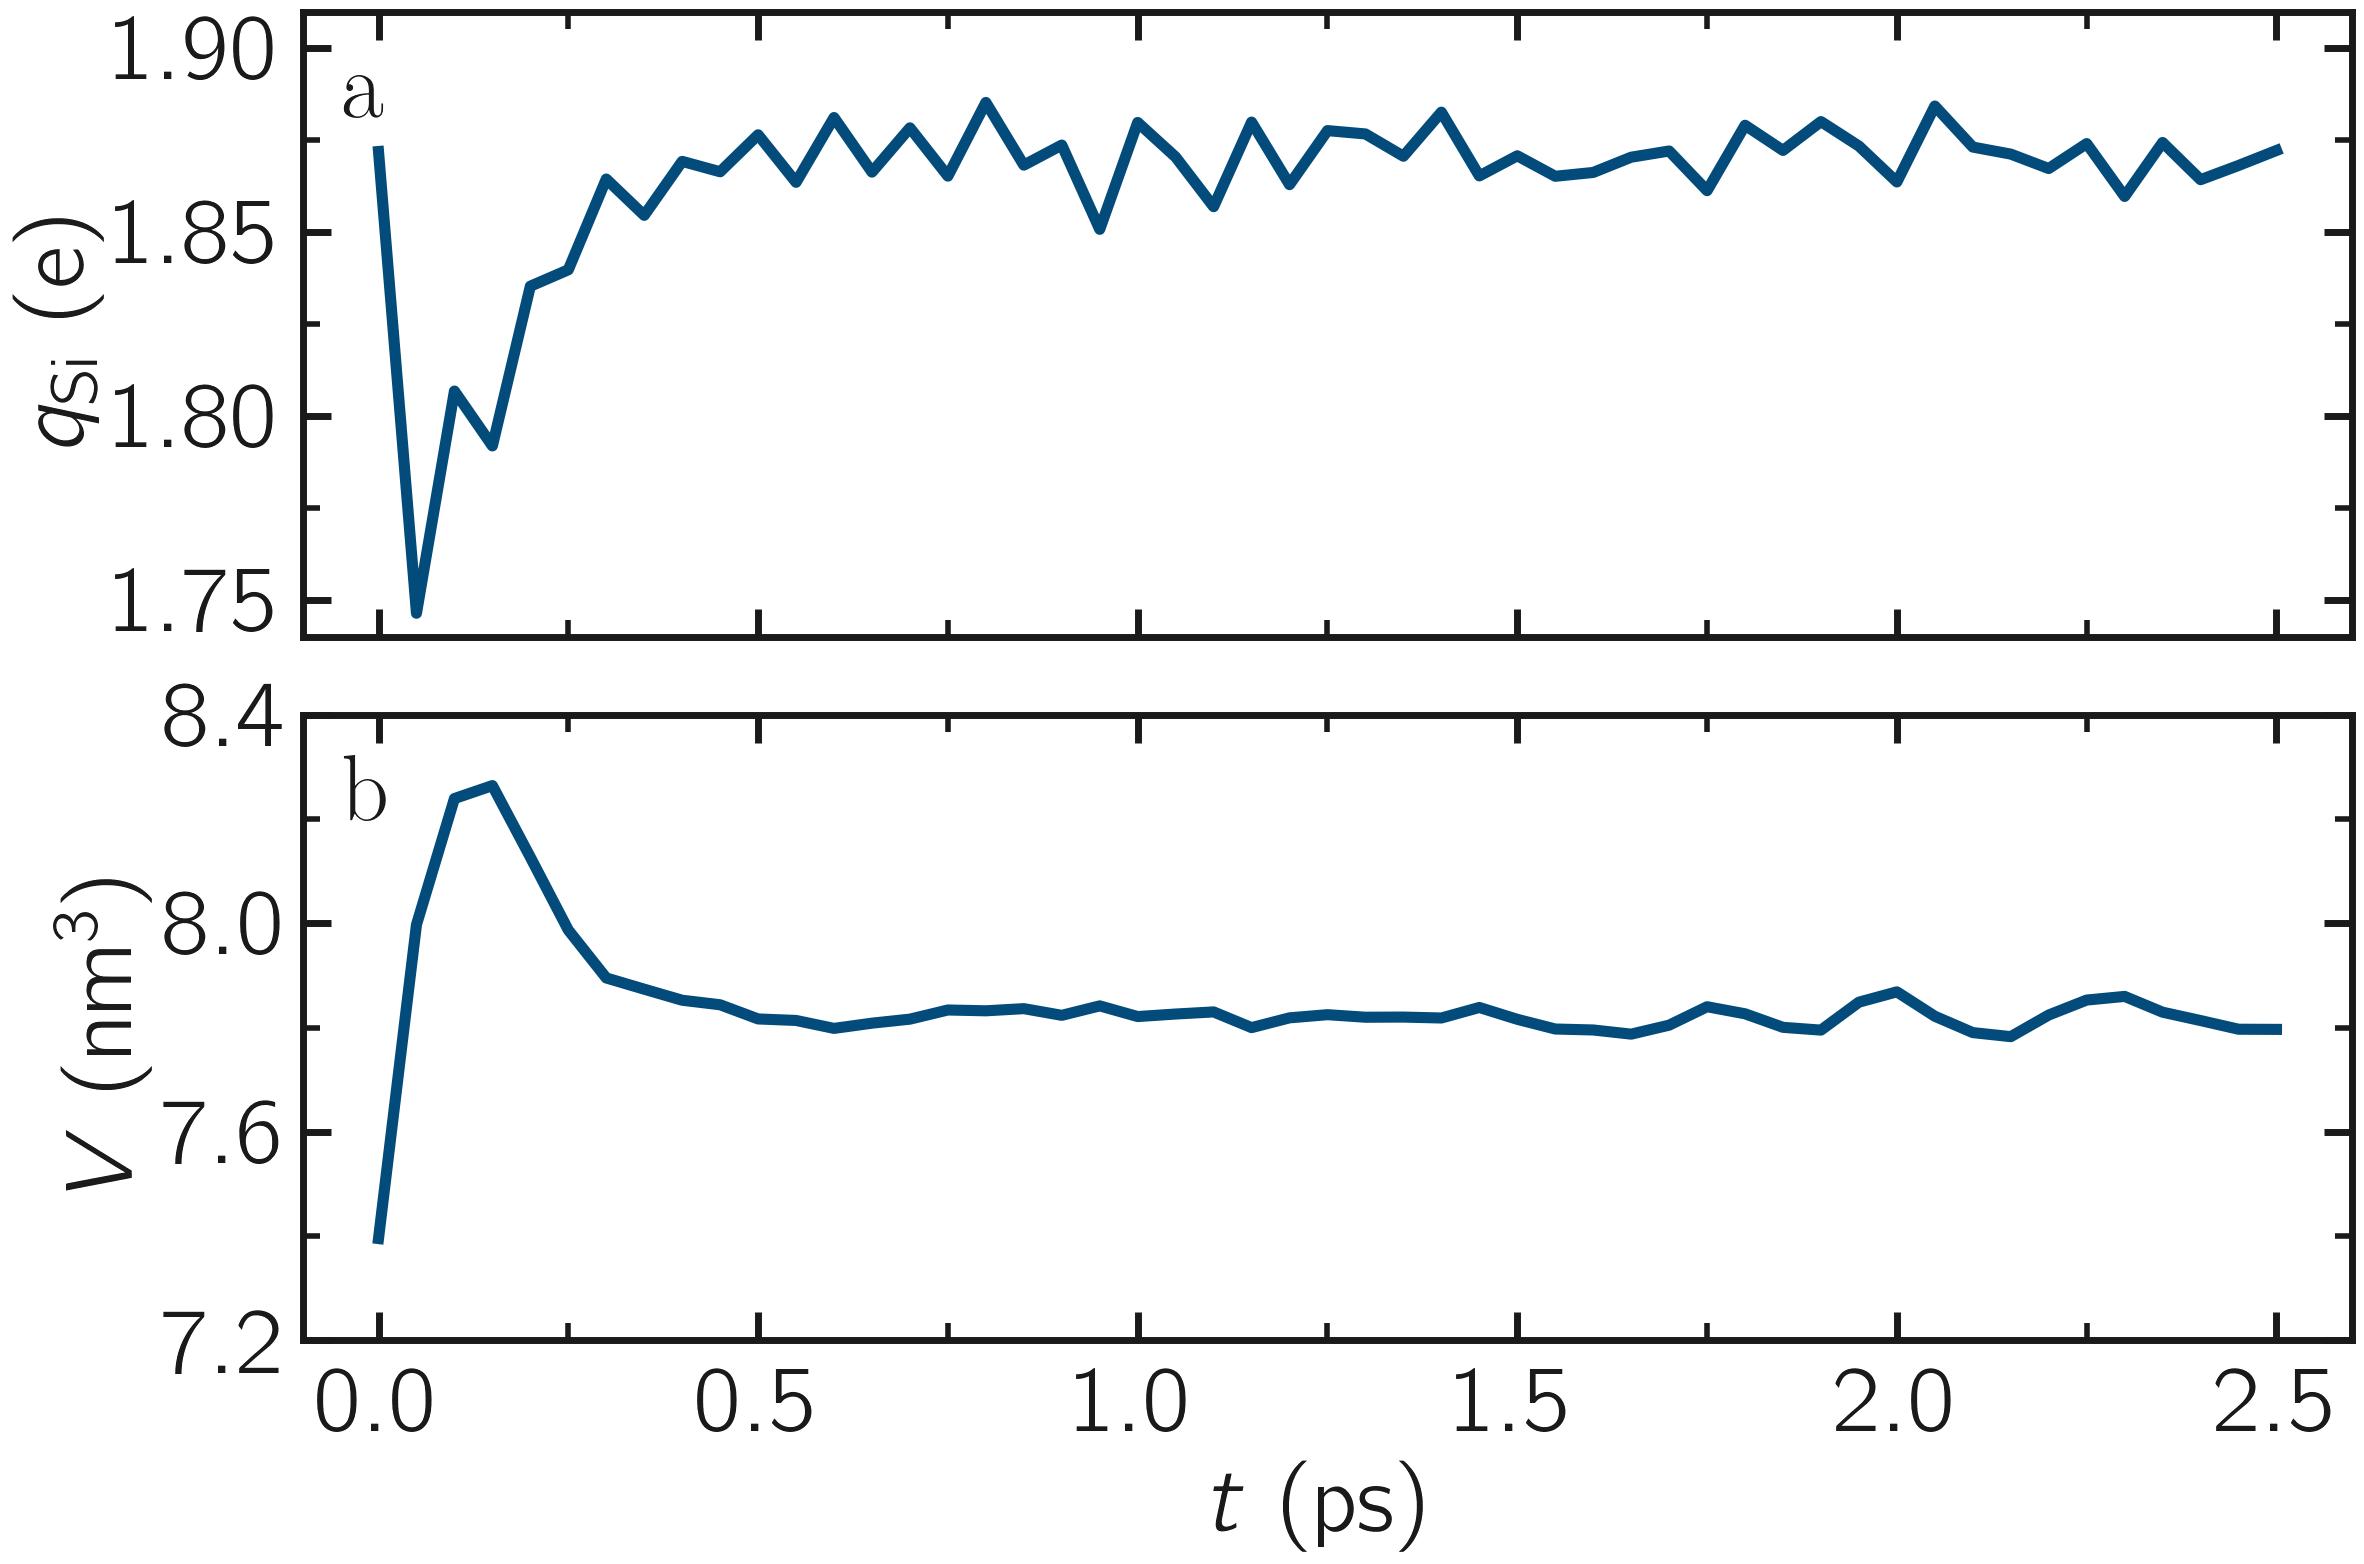
\includegraphics[width=\linewidth]{SIO-charge}
\caption{Average charge per atom of the silicon $q_\text{Si}$ (a) and oxygen
$q_\text{O}$ (b) atoms as a function of time $t$ during equilibration.  $q_\text{Si}$
and $q_\text{O}$ are given by the \textit{v\_qSi} and \textit{v\_qO} variables,
respectively.}
\label{fig:SIO-charge}
\end{figure}

\begin{figure}
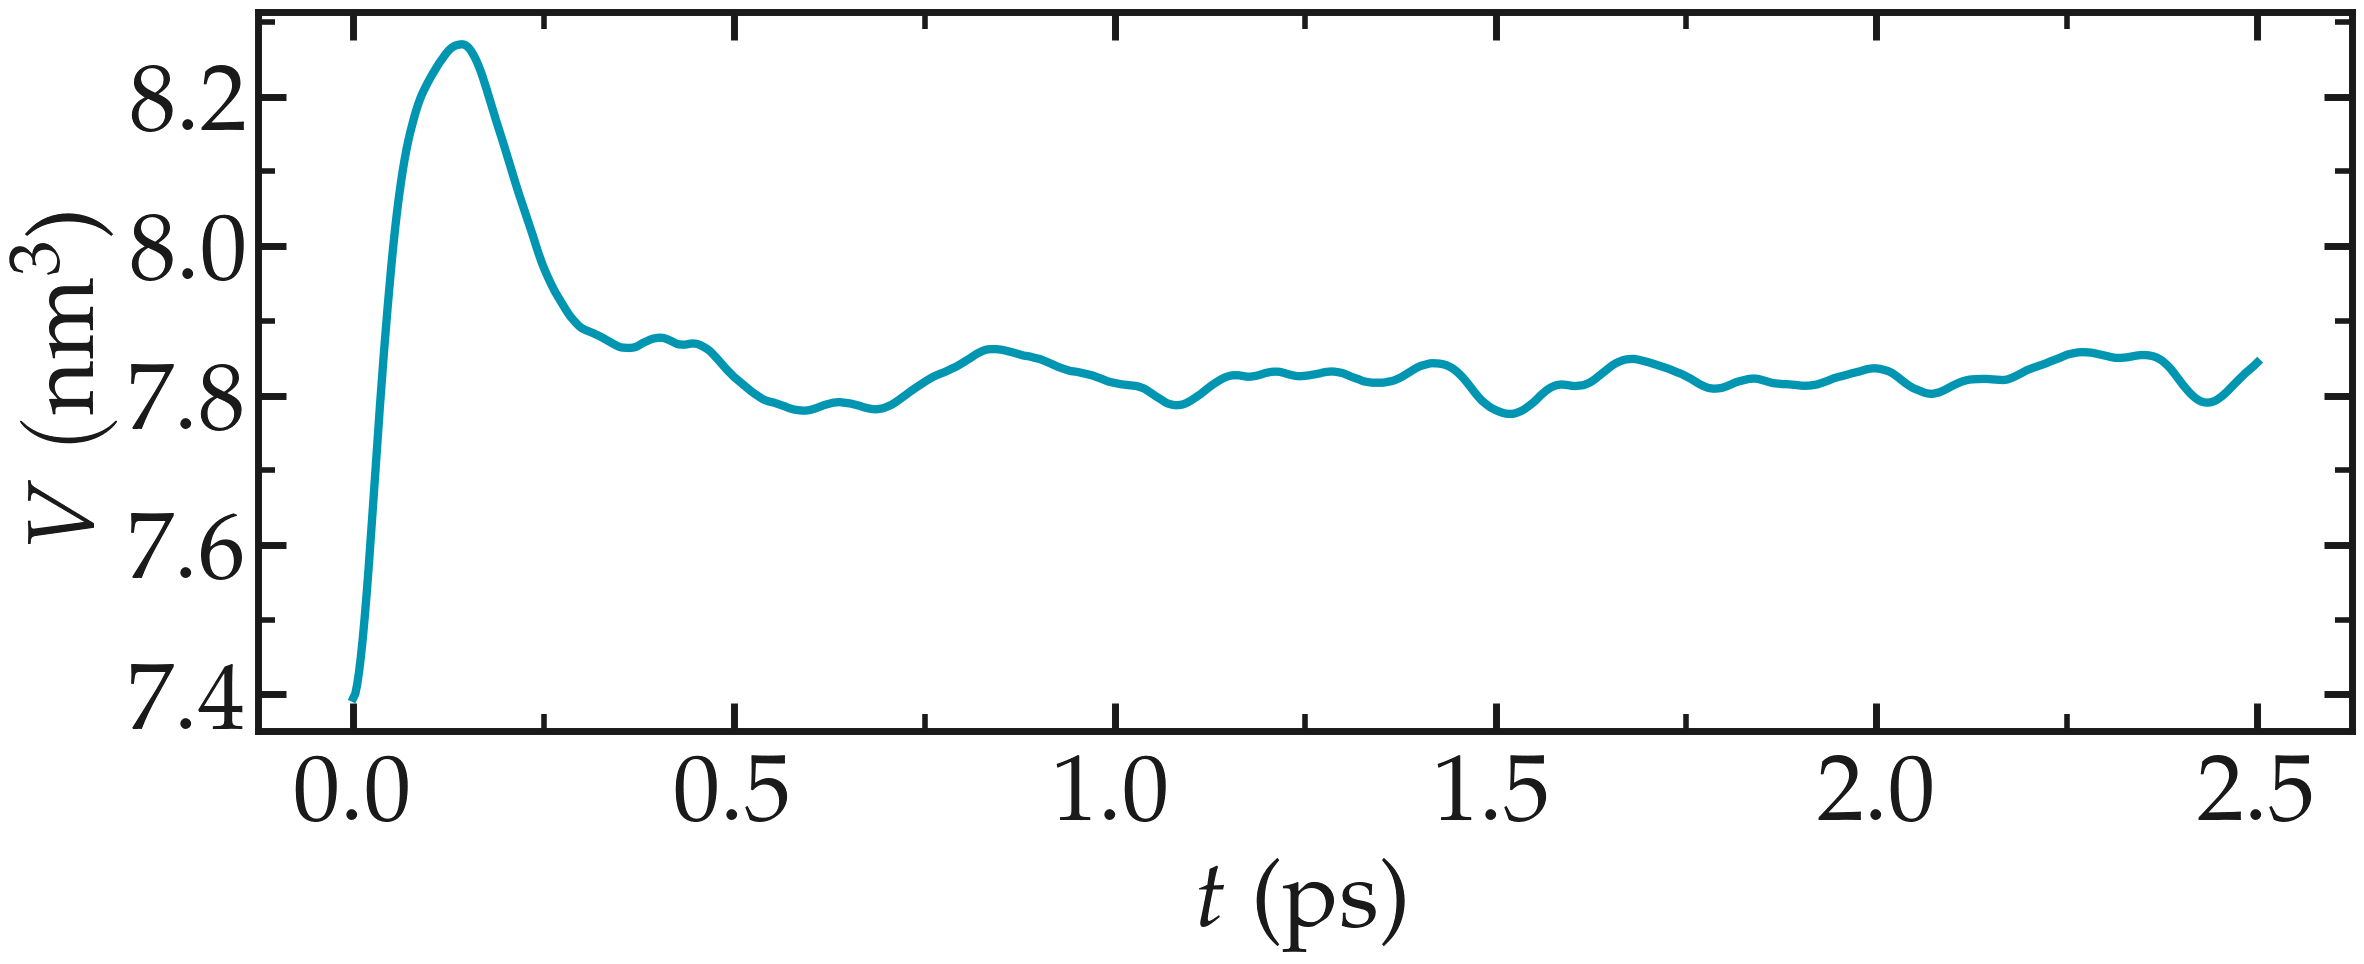
\includegraphics[width=\linewidth]{SIO-volume}
\caption{Volume of the system $V$ as a function of time $t$.}
\label{fig:SIO-volume}
\end{figure}

We can also plot the charge distribution $P(q)$, using the charge values
printed in the \textit{dump.lammptrj} file (Fig.\,\ref{fig:SIO-distribution}).
The \textit{dump.lammptrj} file can be opened using VMD. By coloring the atoms
by their charges, one can see that the atoms with the extreme-most charges are
located at defects in the amorphous structure (here at the positions of the
dangling oxygen groups) (Fig.\,\ref{fig:SIO-slice}).

\begin{figure}
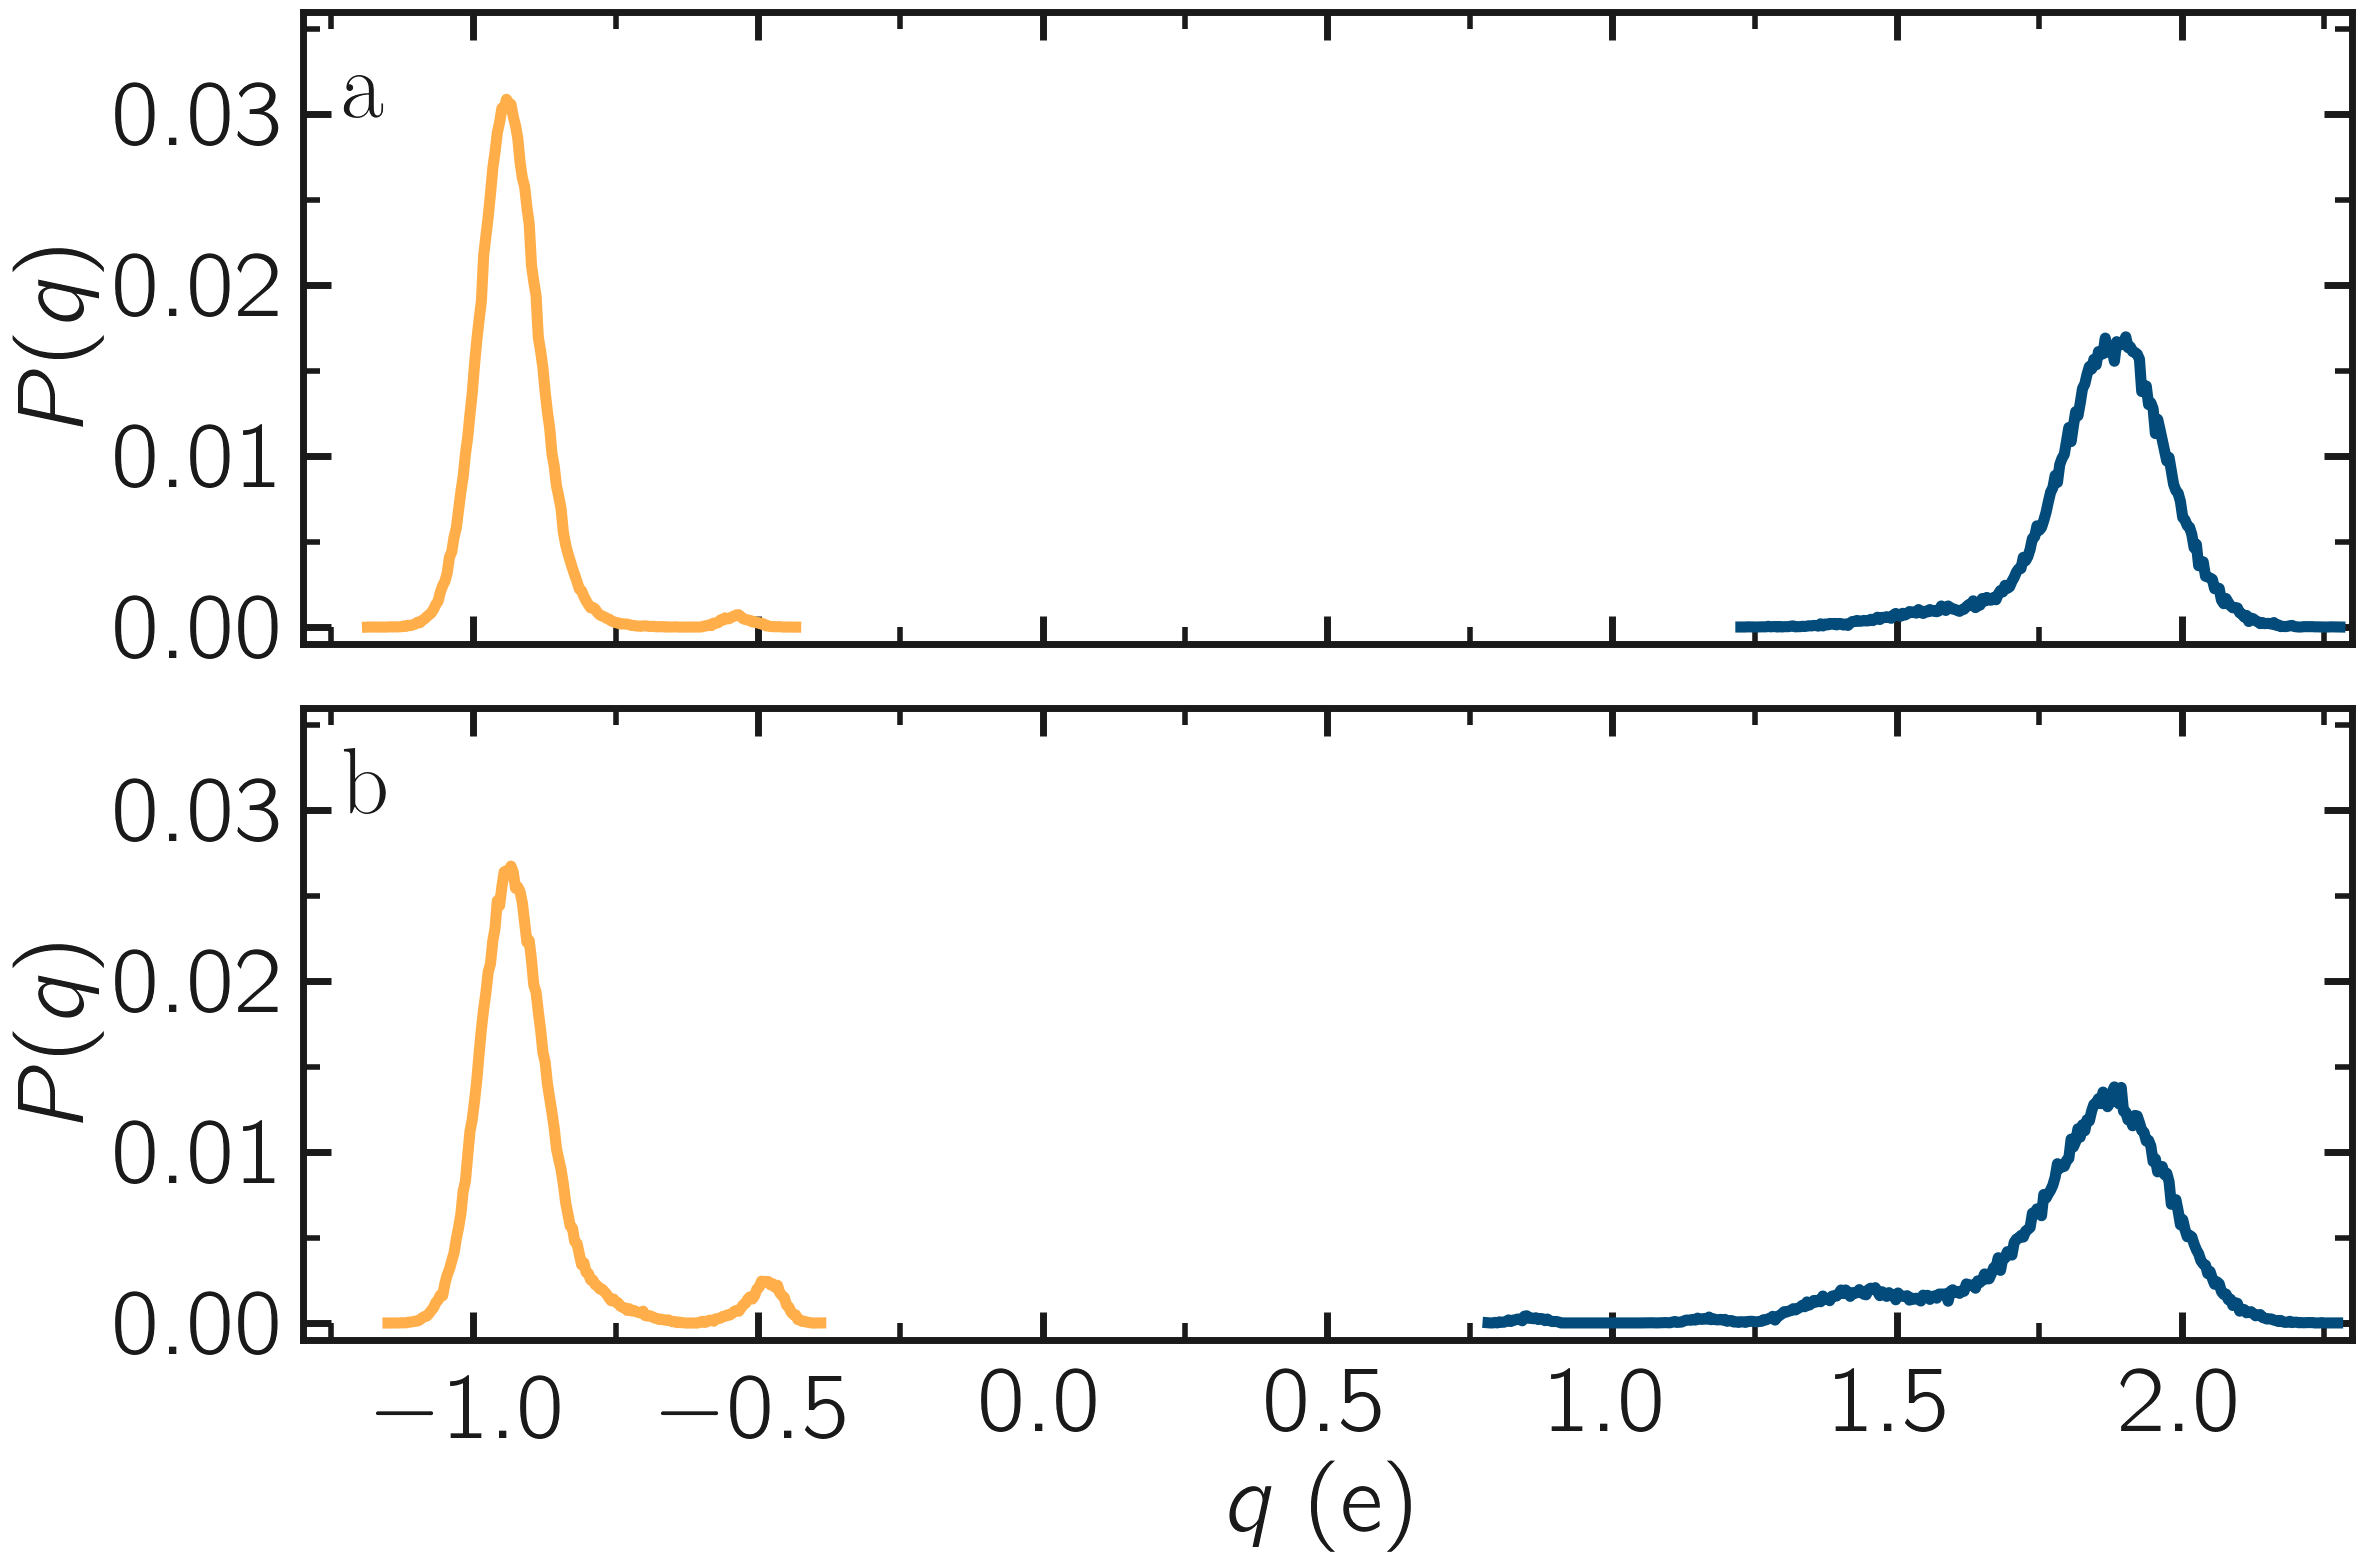
\includegraphics[width=\linewidth]{SIO-distribution}
\caption{Probability distribution of charge of silicon (positive, blue) and oxygen
(negative, orange) atoms during equilibration.}
\label{fig:SIO-distribution}
\end{figure}

\begin{figure}
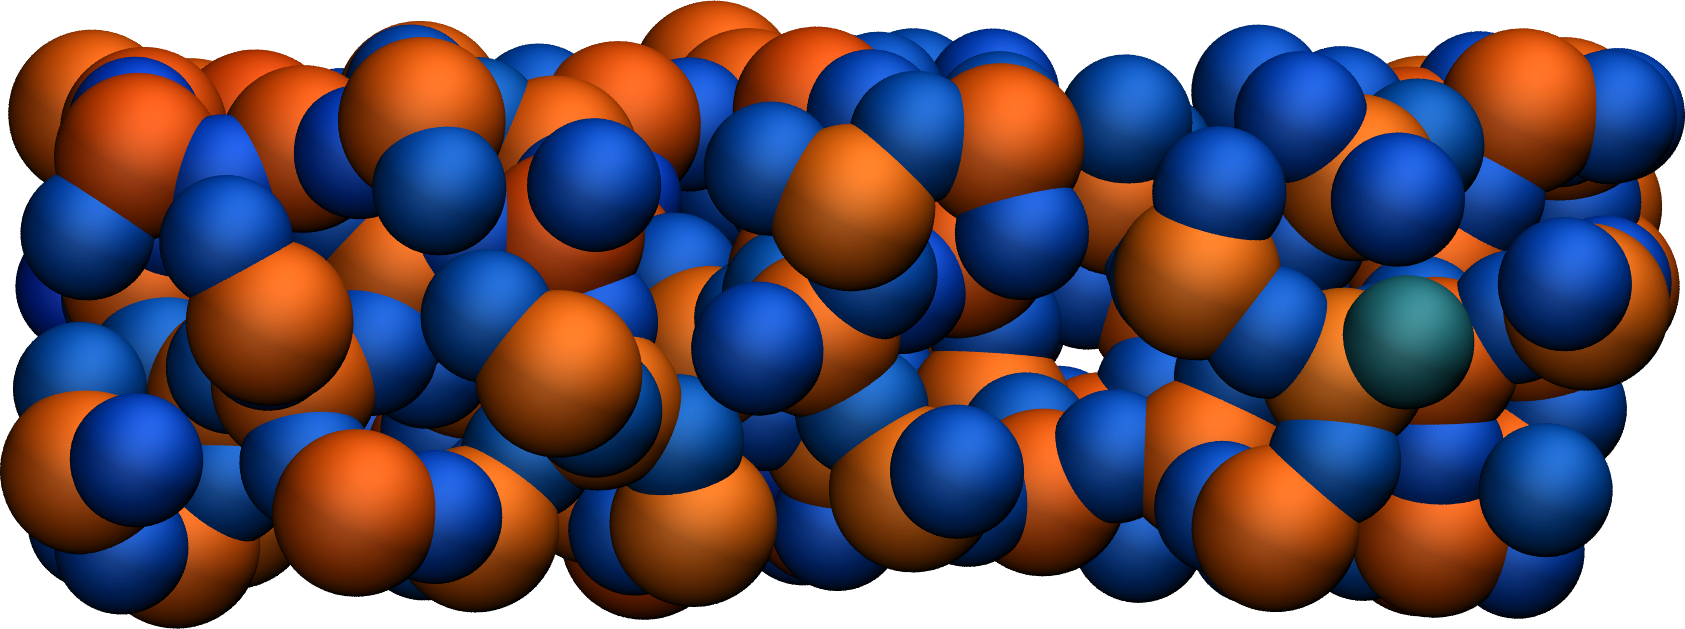
\includegraphics[width=\linewidth]{SIO-slice}
\caption{A slice of the amorphous silica, where atoms are colored by their charges.
Dangling oxygen groups appear in greenish, bulk Si atoms with a charge of about
$1.8~\text{e}$  appear in red/orange, and bulk O atoms with a charge of about
$-0.9~\text{e}$ appear in blue. To color the atoms by their charge using VMD,
use \textit{Charge} as the coloring method in the representation windows, and
then tune the \textit{Color scale} in the \textit{Color control windows}.}
\label{fig:SIO-slice}
\end{figure}

\subsubsection{Deform the structure}
Let us apply a deformation to the structure to force some $\text{Si}-\text{O}$
bonds to break (and eventually re-assemble). Next to \flrcmd{RelaxSilica/},
create a folder, call it \flrcmd{Deform/} and create a file called \flecmd{input.lmp}
in it. Copy the same lines as previously in \flecmd{input.lmp}:
\begin{lstlisting}
units real
atom_style full

read_data ../RelaxSilica/silica-relaxed.data

mass Si 28.0855
mass O 15.999

pair_style reaxff NULL safezone 3.0 mincap 150
pair_coeff * * ../RelaxSilica/reaxCHOFe.ff Si O
fix myqeq all qeq/reaxff 1 0.0 10.0 1.0e-6 &
    reaxff maxiter 400
\end{lstlisting}
The only differences with the previous \flecmd{input.lmp} file are the paths to
the \flecmd{.data} and \flecmd{.ff} files located within \flrcmd{RelaxSilica/}.
Copy the following lines as well:
\begin{lstlisting}
group grpSi type Si
group grpO type O
variable qSi equal charge(grpSi)/count(grpSi)
variable qO equal charge(grpO)/count(grpO)

thermo 200
thermo_style custom step temp etotal &
    press vol v_qSi v_qO

dump mydmp all image 200 dump.*.jpg type type &
    shiny 0.1 box no 0.01 view 0 0 zoom 1.8
dump_modify mydmp backcolor white &
    acolor Si yellow adiam Si 2.5 &
    acolor O red adiam O 2

dump dmp all custom 200 dump.lammpstrj &
    id typelabel q x y z

fix myspec all reaxff/species 5 1 5 species.log &
    element Si O
\end{lstlisting}
Then, let us use \textit{fix nvt} instead of \textit{fix npt} to apply a
thermostat but no barostat:
\begin{lstlisting}
fix mynvt all nvt temp 300.0 300.0 100
timestep 0.5
\end{lstlisting}
Here, no barostat is used because the box volume will be imposed by the \textit{fix deform}.

\begin{figure}
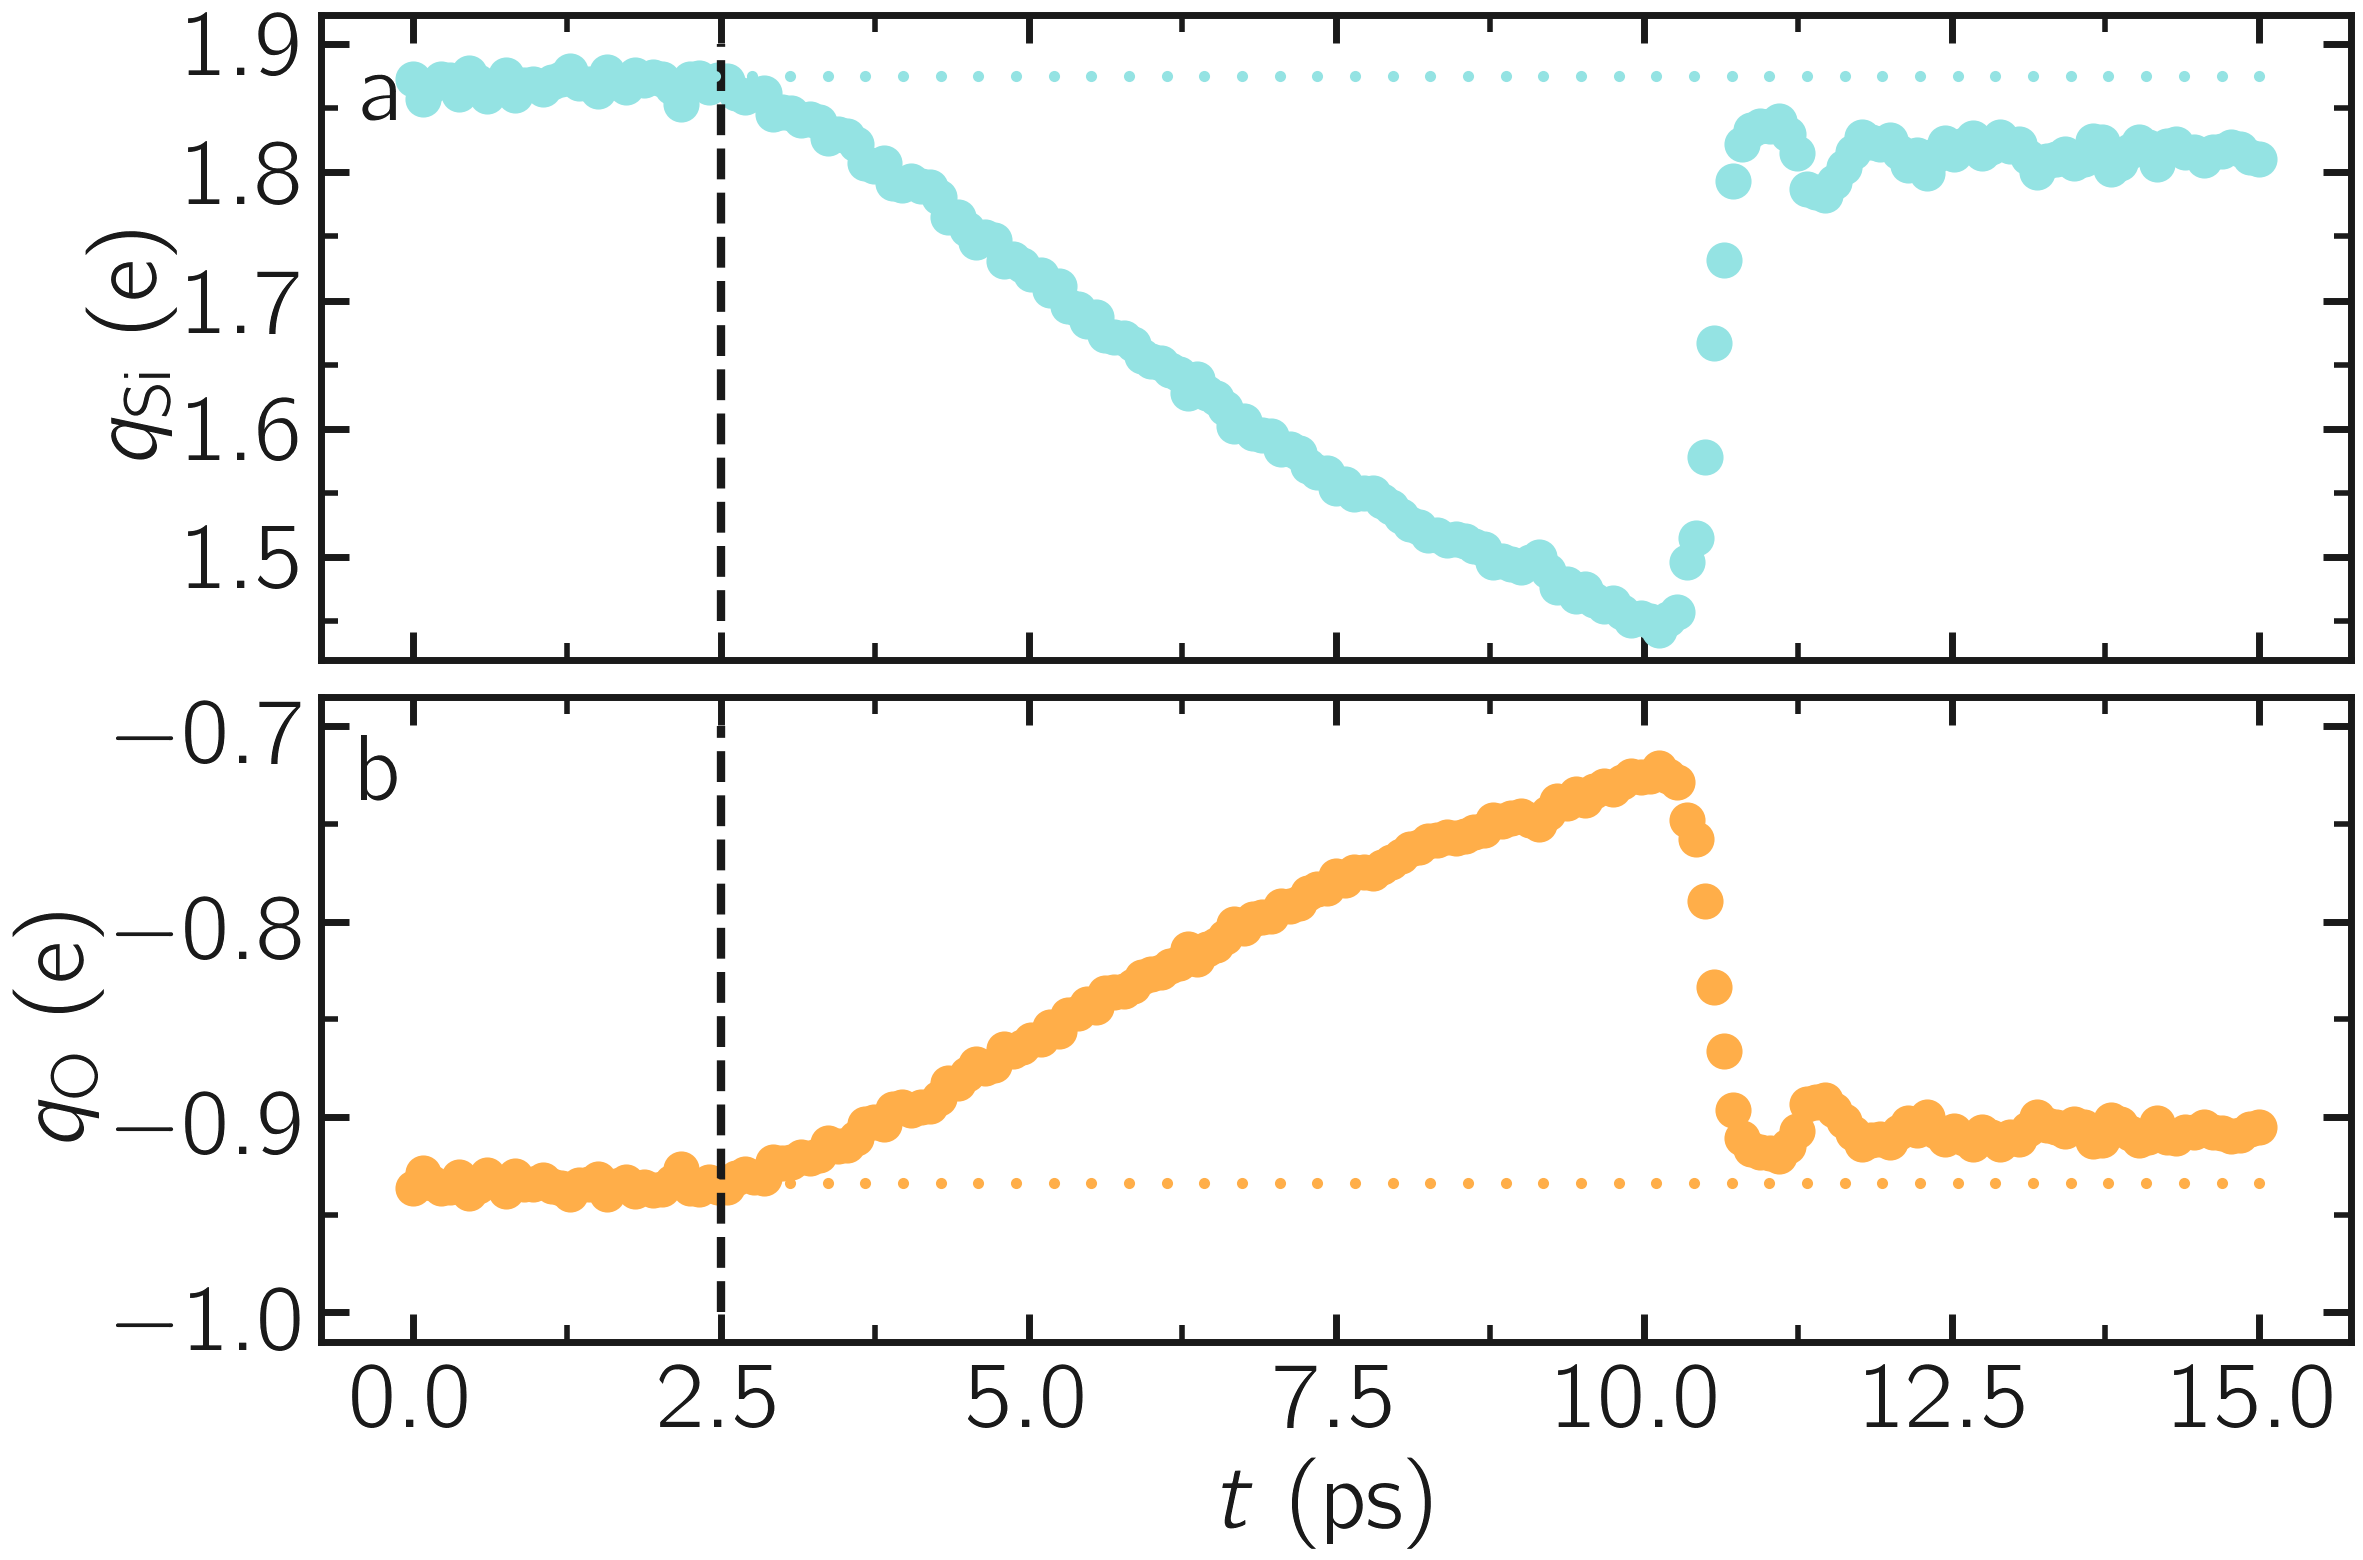
\includegraphics[width=\linewidth]{SIO-deformed-charge}
\caption{Evolution of the average charge per atom of the silicon $q_\text{Si}$
(a) and oxygen $q_\text{O}$ (b) over time $t$. The vertical dashed lines mark
the beginning of the deformation, and the horizontal dotted lines denote the
initial values for the average charge.}
\label{fig:SIO-deformed-charge}
\end{figure}

Let us run for 5000 steps without deformation, then apply the \textit{fix deform}
for elongating progressively the box along \textit{x} during 25000 steps. Add
the following line to \flecmd{input.lmp}:
\begin{lstlisting}
run 5000

fix mydef all deform 1 x erate 5e-5

run 25000

write_data silica-deformed.data
\end{lstlisting}
Run the \flecmd{input.lmp} file using LAMMPS. During the deformation, the charge
values progressively evolve until the structure eventually breaks down. After the
structure breaks down, the charges equilibrate near new average values that differ
from the starting averages (Fig.\,\ref{fig:SIO-deformed-charge}). The difference
between the initial and the final charges can be explained by the presence of
defects as well as new solid/vacuum interfaces, and the fact that surface atoms
typically have different charges compared to bulk atoms. There is also a strong
increase in temperature during the rupture of the material (Fig.\,\ref{fig:SIO-temperature}).
At the end of the deformation, one can visualize the broken material using VMD.
Notice the different charge values of the atoms located near the vacuum interfaces,
compared to the atoms located in the bulk of the material (Fig.\,\ref{fig:SIO-deformed}).

\begin{figure}
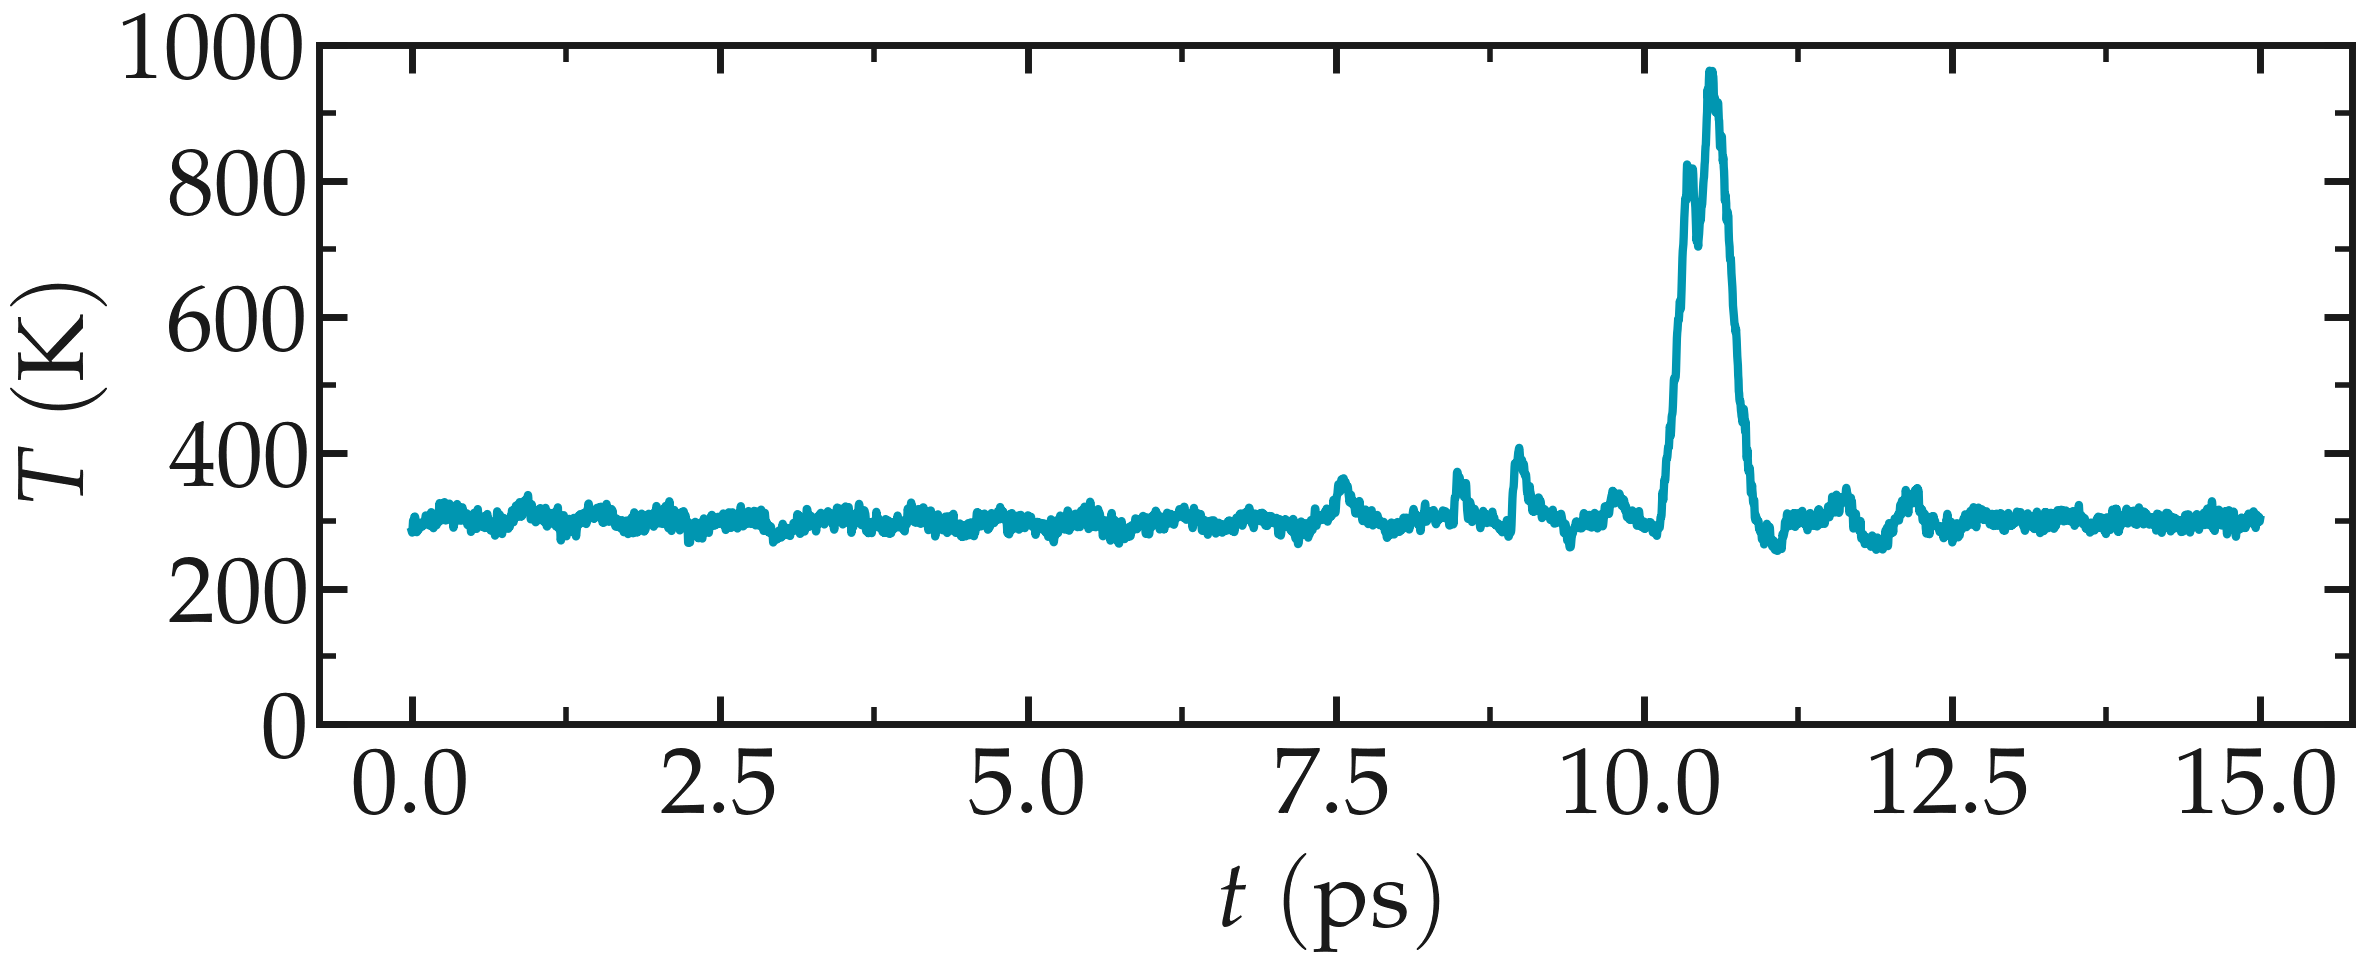
\includegraphics[width=\linewidth]{SIO-temperature}
\caption{Evolution of the temperature $T$ of the silica system over time $t$.
The material ruptures near $t = 10~\text{ps}$.}
\label{fig:SIO-temperature}
\end{figure}

\begin{figure}
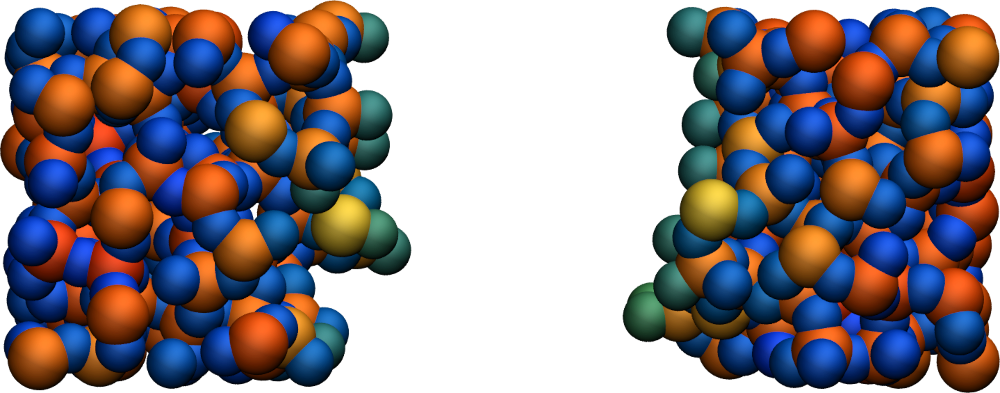
\includegraphics[width=\linewidth]{SIO-deformed}
\caption{Amorphous silicon oxide after deformation. The atoms are colored by their
charges. Dangling oxygen groups appear in greenish, bulk Si atoms with a charge of
about $1.8~\text{e}$  appear in red/orange, and bulk O atoms with a charge of
about $-0.9 ~ \text{e}$ appear in blue.}
\label{fig:SIO-deformed}
\end{figure}

One can have a look at the charge distribution after deformation, as well as during
the deformation (Fig.\,\ref{fig:SIO-distribution-bis}). As expected, the final
charge distribution slightly differs from the previously calculated. If
no new species were formed during the simulation, the \textit{species.log} file
should resemble:
\begin{lstlisting}
#  Timestep   No_Moles   No_Specs  O384Si192
        5            1          1          1
(...)
#  Timestep   No_Moles   No_Specs  O384Si192
    30000            1          1          1
\end{lstlisting}
Sometimes, $\text{O}_2$ molecules are formed during the deformation. If this is
the case, a new column \textit{O2} appears in the \textit{species.log} file.

\begin{figure}
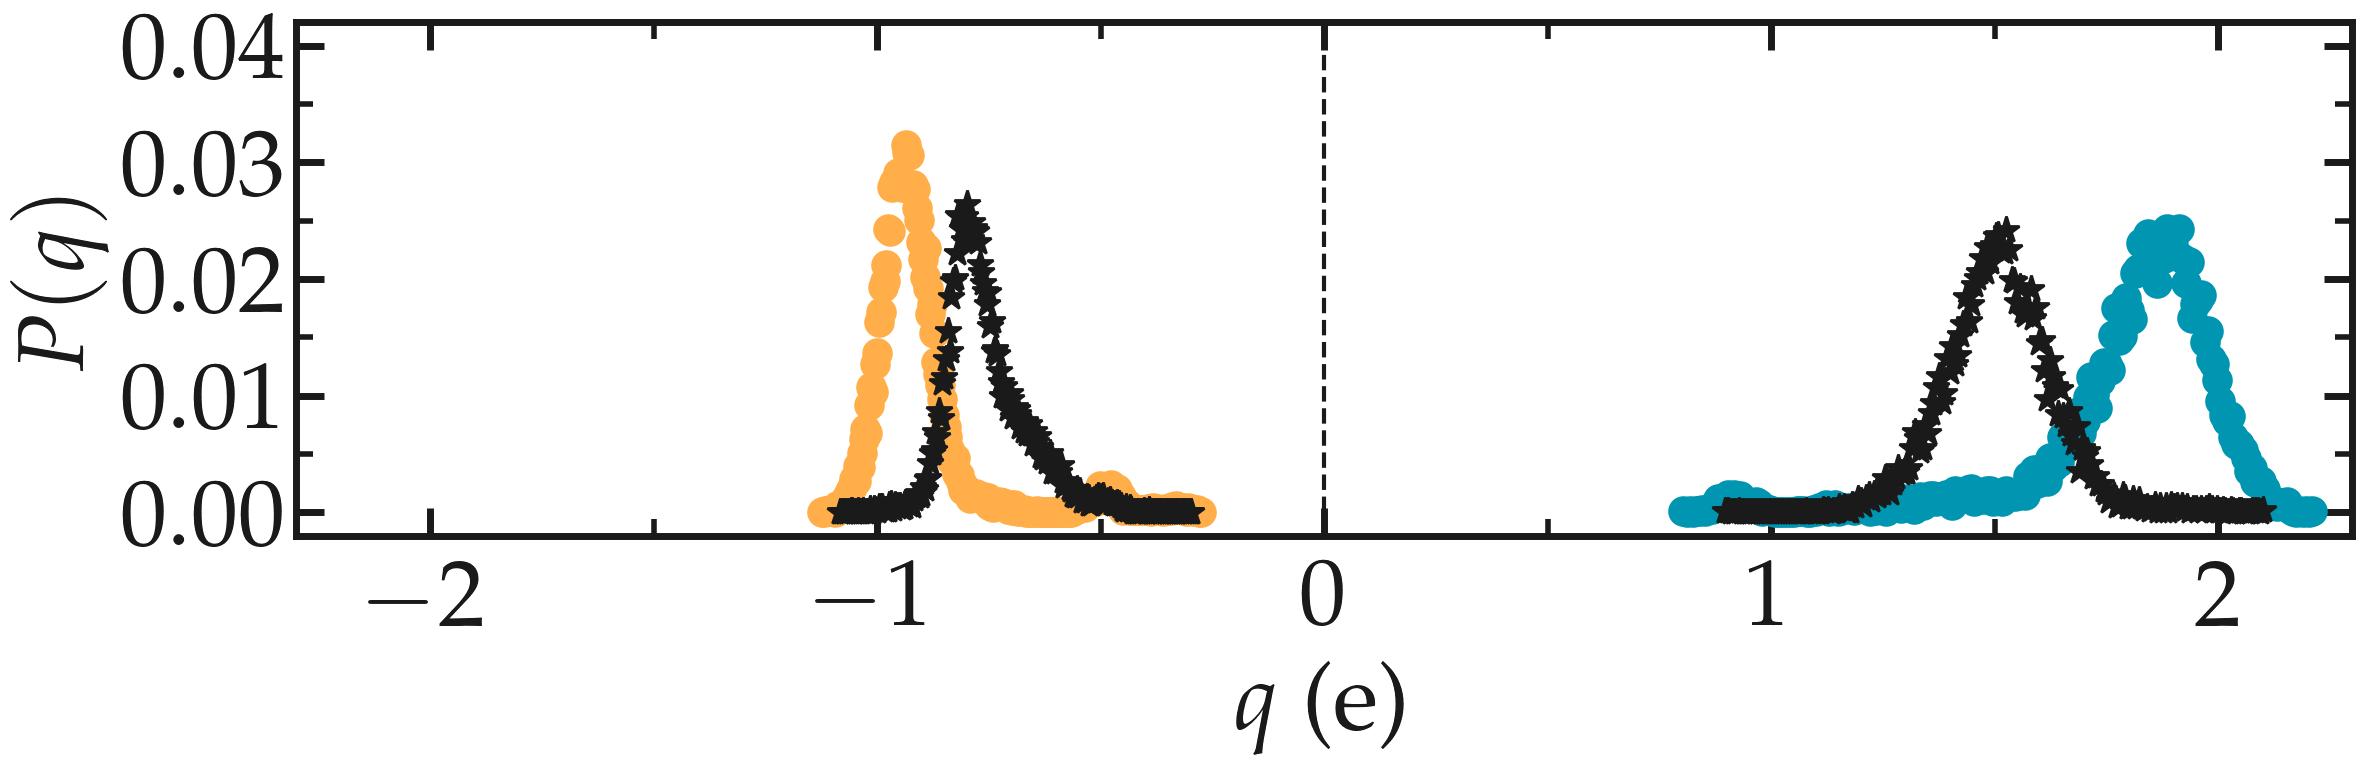
\includegraphics[width=\linewidth]{SIO-distribution-bis}
\caption{Probability distribution of charge of silicon (positive, blue) and oxygen
(negative, orange) after deformation. The stars correspond to the charge distribution
during deformation.}
\label{fig:SIO-distribution-bis}
\end{figure}

\subsubsection{Decorate the surface}
In ambient conditions, some of the surface $\text{SiO}_2$ atoms are chemically
passivated by forming covalent bonds with hydrogen (H) atom \cite{sulpizi2012silica}.
Let us add hydrogen atoms randomly to the cracked silica and observe how the
system evolves.  Next to \flrcmd{RelaxSilica/} and \flrcmd{Deform/}, create a folder,
and call it \flrcmd{Decorate/}. Then, let us modify the previously generated data
file \flecmd{silica-deformed.data} and make space for a third atom type.
Copy \flecmd{silica-deformed.data} from the \flrcmd{Deform/} folder, and modify
the first lines as follows:
\begin{lstlisting}
576 atoms
3 atom types

(...)

Masses

Si 28.0855
O 15.999
H 1.008

(...)
\end{lstlisting}
Create a file called \flecmd{input.lmp} into the \flrcmd{Decorate/} folder, and
copy the following lines into it:
\begin{lstlisting}
units real
atom_style full

read_data silica-deformed.data
displace_atoms all move -12 0 0 # optional

pair_style reaxff NULL safezone 3.0 mincap 150
pair_coeff * * ../RelaxSilica/reaxCHOFe.ff &
    Si O H
fix myqeq all qeq/reaxff 1 0.0 10.0 1.0e-6 &
    reaxff maxiter 400
\end{lstlisting}
Here, the \textit{displace\_atoms} command was used to move the center of the
crack near the center of the box. This step is optional but makes the visualization
of the interface in VMD easier. A different value for the shift may be needed in
your case, depending on the location of the crack. A difference with the previous
input is that three atom types are specified in the \textit{pair\_coeff} command,
\textit{Si O H}, instead of two.

Then, let us adapt some familiar commands to measure the charges of all three
types of atoms, and output the charge values into log files:
\begin{lstlisting}
group grpSi type Si
group grpO type O
group grpH type H
variable qSi equal charge(grpSi)/count(grpSi)
variable qO equal charge(grpO)/count(grpO)
variable qH equal &
    charge(grpH)/(count(grpH)+1e-10)

thermo 5
thermo_style custom step temp etotal press &
    vol v_qSi v_qO v_qH
fix myspec all reaxff/species 5 1 5 &
    species.log element Si O H
\end{lstlisting}
Here, the $+1\text{e}-10$ was added to the denominator of the \textit{variable qH}
to avoid dividing by 0 at the beginning of the simulation. Finally, let us
create a loop with 10 steps, and create two hydrogen atoms at random locations at
every step:
\begin{lstlisting}
fix mynvt all nvt temp 300.0 300.0 100
timestep 0.5

label loop
variable a loop 10

variable seed equal 35672+${a}
create_atoms 3 random 2 ${seed} NULL &
    overlap 2.6 maxtry 50
group grpH type H

run 2000
write_dump all custom dump.${a}.lammpstrj &
    id typelabel q x y z
undump mydmp

next a
jump SELF loop

write_data decorated.data
\end{lstlisting}
Here, a different \textit{lammpstrj} file is created for each step of the loop
to avoid creating dump files with varying numbers of atoms, which VMD can't read.
Once the simulation is over, it can be seen from the \textit{species.log} file that
all the created hydrogen atoms reacted with the $\text{SiO}_{2}$ structure to
form surface groups (such as hydroxyl (-OH) groups).
\begin{lstlisting}
(...)
# Timestep   No_Moles No_Specs H20O384Si192
  20000      1        1        1
\end{lstlisting}
At the end of the simulation, hydroxyl (-OH) groups can be seen at the interfaces
(Fig.\,\ref{fig:SIO-decorated}).

\begin{figure}
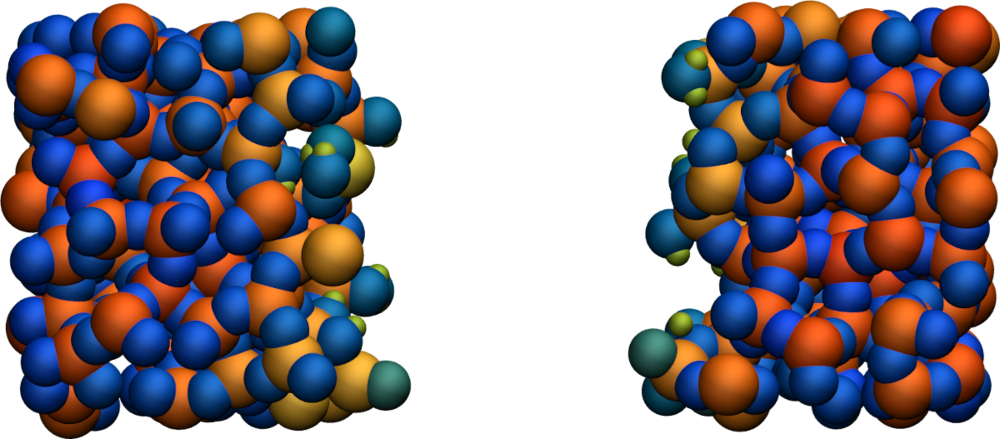
\includegraphics[width=\linewidth]{SIO-decorated}
\caption{Cracked silicon oxide after the addition of hydrogen atoms. The atoms
are colored by their charges. Dangling oxygen groups appear in greenish, bulk
Si atoms with a charge of about $1.8~\text{e}$  appear in red/orange, and bulk
O atoms with a charge of about $-0.9 ~ \text{e}$ appear in blue.}
\label{fig:SIO-decorated}
\end{figure}

\subsection{Tutorial 6: Water adsorption in silica}
\label{gcmc-silica-label}

\begin{figure}
\centering
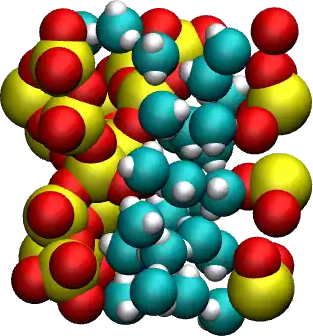
\includegraphics[width=0.55\linewidth]{GCMC}
\caption{Water molecules adsorbed in cracked silica (SiO$_2$) material as simulated
during \hyperref[gcmc-silica-label]{Tutorial 6}. Water molecules are colored in
cyan and white, oxygen (O) atoms from SiO$_2$ in red, and silicon (Si) atoms in yellow.}
\label{fig:GCMC}
\end{figure}

\noindent The objective of this tutorial is to combine molecular dynamics and
grand canonical Monte Carlo simulations to compute the adsorption of water
molecules in cracked silica material (Fig.\,\ref{fig:GCMC}). This tutorial
illustrates the use of the grand canonical ensemble in molecular simulation, an
open ensemble in which the number of atoms or molecules within the simulation
box is not constant. When using the grand canonical ensemble, it is possible to
impose the chemical potential (or pressure) of a given fluid in a nanoporous structure.

\subsubsection{Generation of the silica block}
\noindent Let us first generate a block of amorphous silica ($\text{SiO}_2$).
To do so, we are going to replicate a building block containing 3 Si and 6 O atoms.
Create two folders side by side, and name them respectively \flrcmd{Potential/}
and \flrcmd{SilicaBlock/}. The initial data file for the SiO atoms called
\href{\filepath tutorial6/SiO.data}{\dwlcmd{SiO.data}}
must be downloaded and saved in \flrcmd{SilicaBlock/}. This data file contains
the coordinates of the 9 atoms, their masses, and their charges.

Let us replicate these atoms using LAMMPS, and apply an annealing procedure to
obtain a block of amorphous silica. Create a new input file called \flecmd{input.lmp}
in the \flrcmd{SilicaBlock/} folder, and copy
the following lines into it:
\begin{lstlisting}
units metal
boundary p p p
atom_style full
pair_style vashishta
neighbor 1.0 bin
neigh_modify delay 1
\end{lstlisting}
The main difference from some of the previous tutorials is the use of the \textit{Vashishta}
pair style. The Vashishta potential is a bond-angle energy-based potential, it deduces
the bonds between atoms from their relative positions \cite{vashishta1990interaction}.

Let us then import the system consisting of 9 atoms, and replicate it four times
in all three directions of space, thus creating a system with 576 atoms. Add the
following lines into \flecmd{input.lmp}:
\begin{lstlisting}
read_data SiO.data
replicate 4 4 4
\end{lstlisting}
Then, let us specify the pair coefficients by indicating that the first atom type
is \textit{Si} and the second is \textit{O}. Let us also add a dump command to
print out the positions of the atoms every 5000 steps:
\begin{lstlisting}
pair_coeff * * &
    ../Potential/SiO.1990.vashishta Si O
\end{lstlisting}
Download the \href{\filepath tutorial6/SiO.1990.vashishta}{\dwlcmd{SiO.1990.vashishta}},
and copy it within the \flrcmd{Potential/} folder.

Let us add a \textit{dump image} command to \flecmd{input.lmp} to follow the
evolution of the system with time:
\begin{lstlisting}
dump mydmp all image 200 dump.*.jpg type type &
    shiny 0.1 box no 0.01 view 0 0 zoom 1.2
dump_modify mydmp backcolor white &
    acolor Si yellow adiam Si 2.5 &
    acolor O red adiam O 2
thermo 1000
thermo_style custom step temp etotal &
    vol lx ly lz
\end{lstlisting}
Thanks to the \textit{thermo\_style custom} command, the box size along each direction
will be printed in the log file.

Finally, let us create the last part of our script. The annealing procedure is
made of four consecutive runs. First, a $50\,\text{ps}$ phase at $T = 6000\,\text{K}$
and isotropic pressure coupling with desired pressure $p = 100\,\text{atm}$:
\begin{lstlisting}
velocity all create 6000 4928459 &
    rot yes dist gaussian
fix npt1 all npt temp 6000 6000 0.1 &
    iso 100 100 1
timestep 0.001
run 50000
\end{lstlisting}
Then, a second phase during which the system is cooled down from $T = 6000\,\text{K}$
to $T = 4000\,\text{K}$. An anisotropic pressure coupling is used, allowing all
three dimensions of the box to evolve independently from one another:
\begin{lstlisting}
fix npt1 all npt temp 6000 4000 0.1 &
    aniso 100 100 1
run 50000
\end{lstlisting}
Then, let us cool down the system further while also reducing the pressure, and then
perform a small equilibration step at the final desired condition, $T = 300\,\text{K}$ and $p = 1\,\text{atm}$.
\begin{lstlisting}
fix npt1 all npt temp 4000 300 0.1 &
    aniso 100 1 1
run 200000
fix npt1 all npt temp 300 300 0.1 &
    aniso 1 1 1
run 50000
write_data amorphousSiO.data
\end{lstlisting}
Here, an isotropic barostat is used for the melted phase at $T = 6000\,\text{K}$,
and an anisotropic barostat is used for all following phases. With the anisotropic
barostat, all three directions of space are adjusted independently from one another.
An anisotropic barostat is usually a better choice for a solid phase. For a liquid
or a gas, an isotropic barostat is usually the best choice.

Run the simulation using LAMMPS. From the \textit{Charts} window, the temperature
can be seen to follow well the desired annealing procedure (Fig.\,\ref{fig:GCMC-temperature}).
The evolution of the box dimensions over time confirms that the box was indeed
deformed isotropically during the first stage of the simulation, and then anisotropically
(Fig.\,\ref{fig:GCMC-dimension}). After running
the simulation, the final LAMMPS topology file called \flecmd{amorphousSiO.data}
will be located in \flrcmd{SilicaBlock/} (Fig.\,\ref{fig:GCMC-snapshot}).

\begin{figure}
\centering
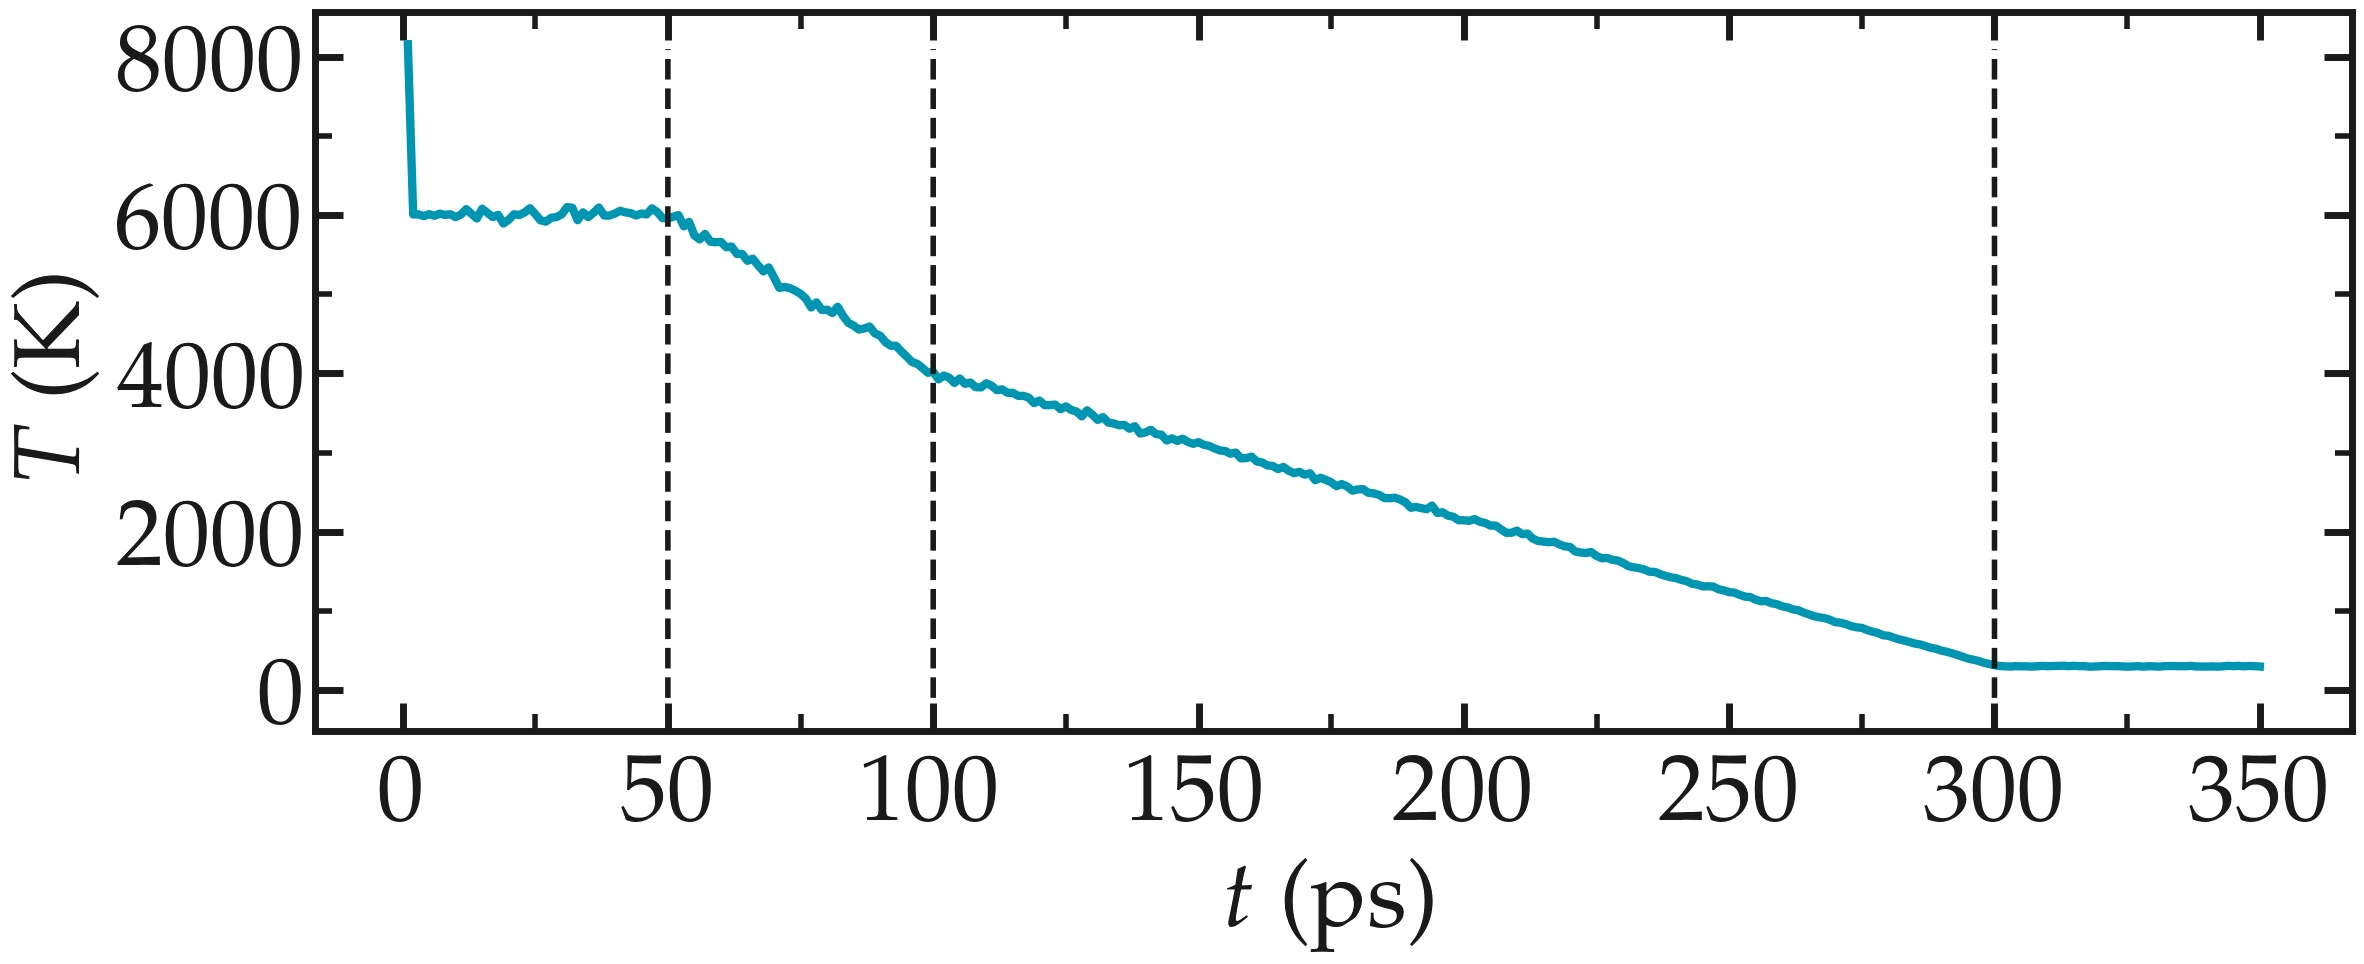
\includegraphics[width=\linewidth]{GCMC-temperature}
\caption{Temperature $T$ of the system during annealing. The vertical dashed lines
mark the transition between the different phases of the simulation.}
\label{fig:GCMC-temperature}
\end{figure}

\begin{figure}
\centering
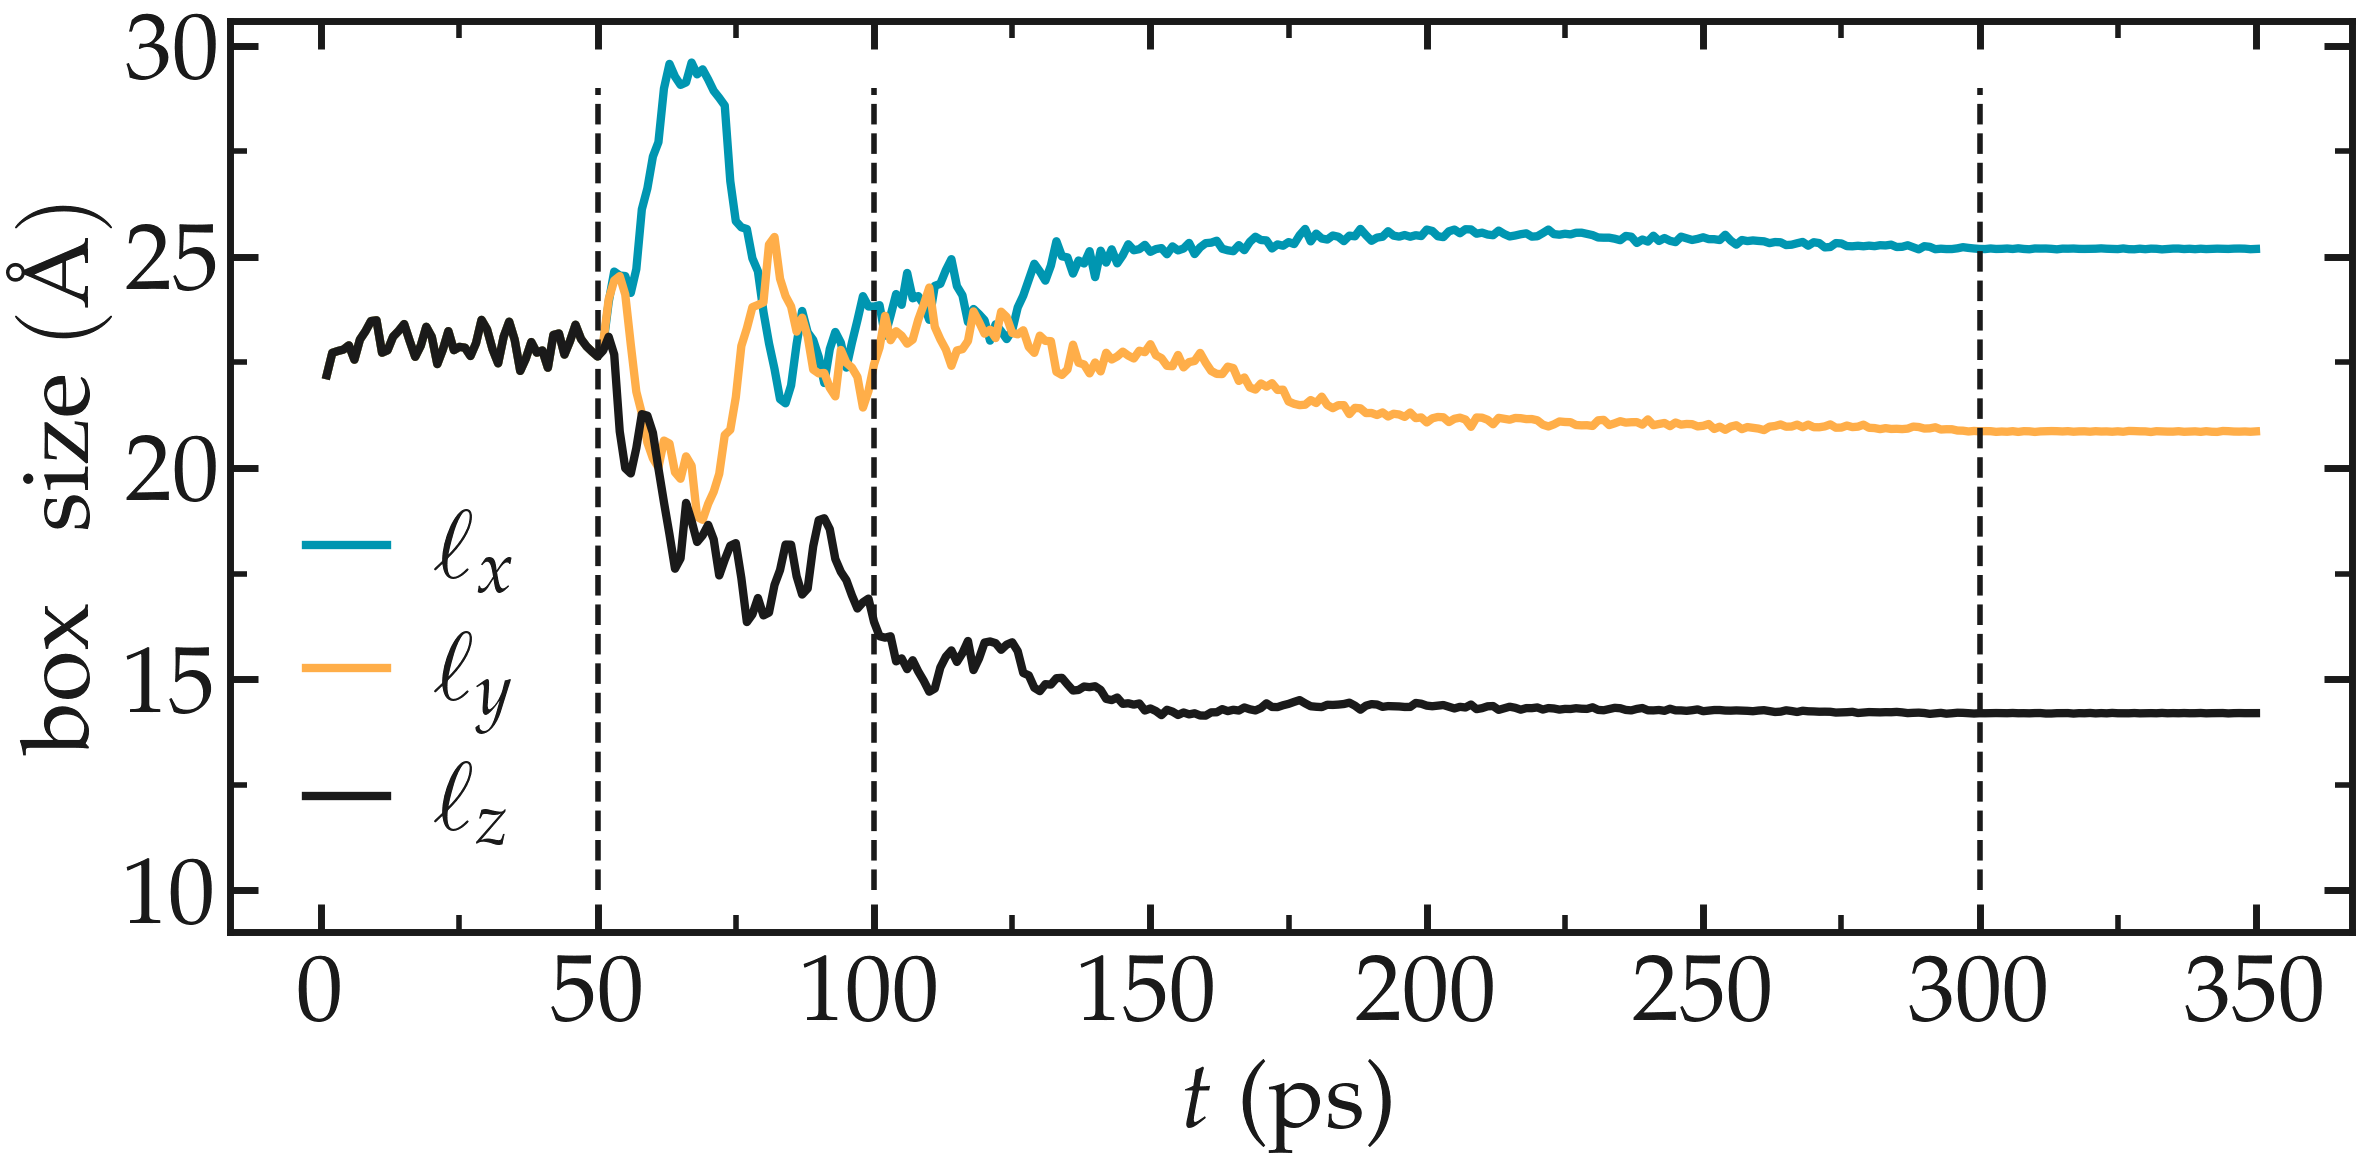
\includegraphics[width=\linewidth]{GCMC-dimension}
\caption{Box dimensions along $x$ (blue), $y$ (orange), and $z$ (dark) during
annealing. The vertical dashed lines mark the transition between the different
phases of the simulation.}
\label{fig:GCMC-dimension}
\end{figure}

\begin{figure}
\centering
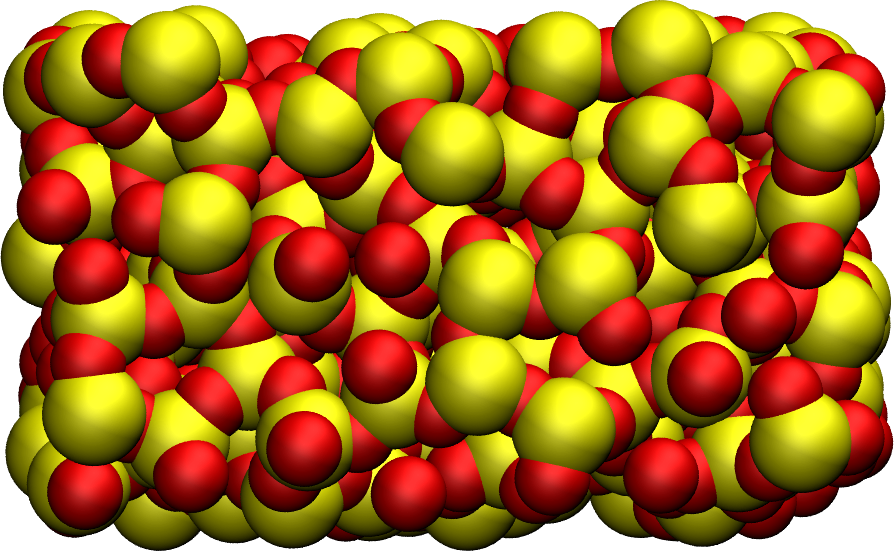
\includegraphics[width=0.9\linewidth]{GCMC-snapshot}
\caption{Final amorphous silica ($\text{SiO}_2$). The silicon atoms are
represented in yellow, and the oxygen atoms in red.}
\label{fig:GCMC-snapshot}
\end{figure}

\subsubsection{Cracking the silica}
Let us dilate the block of silica until a crack forms. Create a new folder
called \flrcmd{Cracking/} next to \flrcmd{SilicaBlock/}, as well as a new
\flecmd{input.lmp} file starting with familiar lines as previously:
\begin{lstlisting}
units metal
boundary p p p
atom_style full
neighbor 1.0 bin
neigh_modify delay 1

read_data ../SilicaBlock/amorphousSiO.data

pair_style vashishta
pair_coeff * * &
    ../Potential/SiO.1990.vashishta Si O
dump dmp all atom 1000 dump.lammpstrj
\end{lstlisting}
Let us progressively increase the size of the box in the $x$ direction, thus forcing
the silica to deform and eventually crack. To do so, a loop based on the jump command
is used. At every step of the loop, the box dimension over $x$ will be multiplied
by a scaling factor 1.005. Add the following lines into the \flecmd{input.lmp}:
\begin{lstlisting}
fix nvt1 all nvt temp 300 300 0.1
timestep 0.001
thermo 1000
variable var loop 45
label loop
change_box all x scale 1.005 remap
run 2000
next var
jump input.lmp loop
run 20000
write_data dilatedSiO.data
\end{lstlisting}
The \textit{fix nvt} is used to control the temperature of the system, while the
\textit{change\_box} command imposes incremental deformations of the box. Different
scaling factors or different numbers of steps can be used to generate different
defects in the silica. After the expansion, a final equilibration step of a duration
of 20 picoseconds is performed. If you look at the \textit{dump.lammpstrj} file
using VMD, you can see the expansion occurring step-by-step, and the atoms
progressively adjusting to the box dimensions. At first, the deformations are
reversible (elastic regime). At some point, bonds start breaking and dislocations
appear (plastic regime). The final system is shown in Fig.\,\ref{fig:GCMC-cracked}.

\begin{figure}
\centering
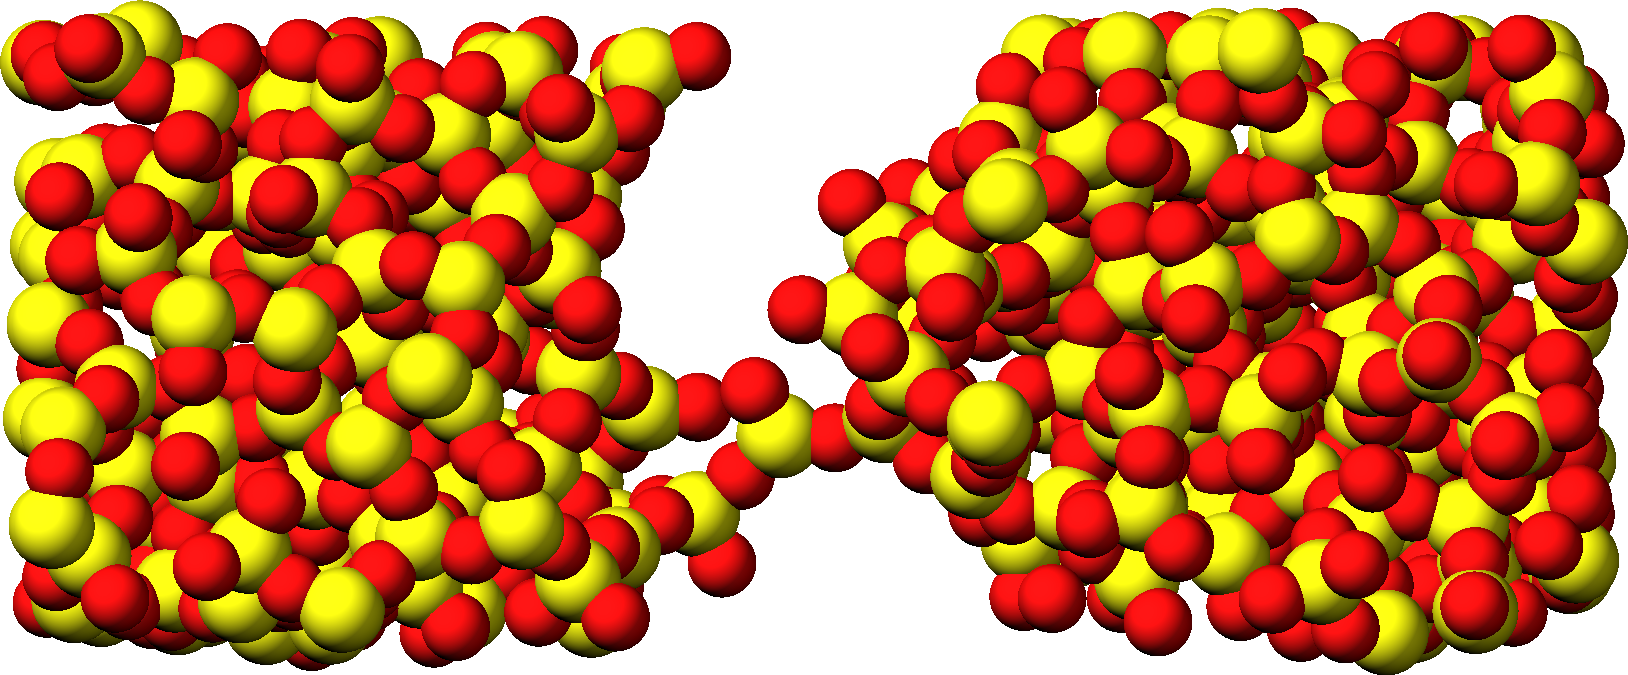
\includegraphics[width=\linewidth]{GCMC-cracked}
\caption{Block of silica after deformation. The silicon atoms are represented in
yellow, and the oxygen atoms in red. Some holes are visible.}
\label{fig:GCMC-cracked}
\end{figure}

\subsubsection{Adding water}
\noindent In order to add the water molecules to the silica, we are going to use
the Monte Carlo method in the grand canonical ensemble (GCMC). In short, the
system is put into contact with a virtual reservoir of a given chemical potential
$\mu$, and multiple attempts to insert water molecules at random positions are
made. Each attempt is either accepted or rejected based on energy considerations.
Find more details in classical textbooks like Ref.~\citenum{frenkel2023understanding}.

\paragraph{Using hydrid potentials}
\noindent Create a new folder called \flrcmd{Addingwater/}. Download and save
the water molecule template called
\href{\filepath tutorial6/H2O.mol}{\dwlcmd{H2O.mol}}
within the \flrcmd{Addingwater/} folder. Create a new input file called \flecmd{input.lmp}
within \flrcmd{Addingwater/}, and copy the following lines into it:
\begin{lstlisting}
units metal
boundary p p p
atom_style full
neighbor 1.0 bin
neigh_modify delay 1
pair_style hybrid/overlay vashishta &
    lj/cut/tip4p/long OW HW OW-HW HW-OW-HW &
    0.1546 10
kspace_style pppm/tip4p 1.0e-4
bond_style harmonic
angle_style harmonic
\end{lstlisting}
There are several differences with the previous input files used in this tutorial.
From now on, the system will combine water and silica, and therefore two force
fields are combined: Vashishta for $\text{SiO}_2$, and lj/cut/tip4p/long for
TIP4P water model (here the TIP4P/2005 model is used \cite{abascal2005general}).
Combining the two force fields is done using the \textit{hybrid/overlay} pair
style. The PPPM solver \cite{luty1996calculating} is set with the \textit{kspace}
command, and is used to calculate the long-range Coulomb interactions associated
with \textit{tip4p/long}. Finally, the style for the bonds
and angles of the water molecules are defined, although they are not important
since TIP4P/2005 is a rigid water model.

Before going further, we also need to make a few changes to our data file.
Currently, \flecmd{dilatedSiO.data} only includes two atom types, but we need four.
Copy the previously generated \flecmd{dilatedSiO.data} file within \flrcmd{Addingwater/}.
Currently, \flecmd{dilatedSiO.data} starts with:
\begin{lstlisting}
576 atoms
2 atom types

-3.517115256285223 24.10269296788487 xlo xhi
0.5721674106566077 20.013410300943264 ylo yhi
1.3237302567479095 19.261847454851658 zlo zhi

Masses

Si 28.0855
O 15.9994

Atoms # full

(...)
\end{lstlisting}
Make the following changes to allow for the addition of water molecules. Modify
the file so that it looks like the following (with 4 atom types, 1 bond type,
1 angle type, and four masses):
\begin{lstlisting}
576 atoms
4 atom types
1 bond types
1 angle types

2 extra bond per atom
1 extra angle per atom
2 extra special per atom

-3.517115256285223 24.10269296788487 xlo xhi
0.5721674106566077 20.013410300943264 ylo yhi
1.3237302567479095 19.261847454851658 zlo zhi

Atom Type Labels

1 Si
2 O
3 OW
4 HW

Bond Type Labels

1 OW-HW

Angle Type Labels

1 HW-OW-HW

Masses

Si 28.0855
O 15.9994
OW 15.9994
HW 1.008

Atoms # full

(...)
\end{lstlisting}
Doing so, we anticipate that there will be 4 atom types in the simulations,
with O and H of $\text{H}_2\text{O}$ having types OW and HW, respectively. There
will also be 1 bond type and 1 angle type. The extra bond, extra angle, and
extra special lines are here for memory allocation. We can continue to fill in
the \flecmd{input.lmp} file, by adding the system definition:
\begin{lstlisting}
read_data dilatedSiO.data
molecule h2omol H2O.mol
lattice sc 3
create_atoms 0 box mol h2omol 45585
lattice none 1

group SiO type Si O
group H2O type OW HW
\end{lstlisting}
After reading the data file and defining the h2omol molecule from the \flecmd{H2O.txt}
file, the \textit{create\_atoms} command is used to include some water molecules
in the system on a simple cubic lattice. Not adding a molecule before starting
the GCMC steps usually leads to failure. Note that here, most water molecules
overlap with the silica. These overlapping water molecules will have to be
deleted before starting the simulation (see below). Then, add the following
settings to \flecmd{input.lmp}:
\begin{lstlisting}
pair_coeff * * vashishta &
    ../Potential/SiO.1990.vashishta &
    Si O NULL NULL
pair_coeff * * lj/cut/tip4p/long 0 0
pair_coeff Si OW lj/cut/tip4p/long 0.0057 4.42
pair_coeff O OW lj/cut/tip4p/long 0.0043 3.12
pair_coeff OW OW lj/cut/tip4p/long 0.008 3.1589
pair_coeff HW HW lj/cut/tip4p/long 0.0 0.0
bond_coeff OW-HW 0 0.9572
angle_coeff HW-OW-HW 0 104.52
\end{lstlisting}
The force field Vashishta applies only to Si and O of $\text{SiO}_2$,
and not to the O and H of $\text{H}_2\text{O}$, thanks to the NULL parameters
used for atoms of types OW and HW. Pair coefficients for the lj/cut/tip4p/long
potential are defined between O($\text{H}_2\text{O}$) and between H($\text{H}_2\text{O}$)
atoms, as well as between O($\text{SiO}_2$)-O($\text{H}_2\text{O}$) and
Si($\text{SiO}_2$)-O($\text{H}_2\text{O}$). Therefore, the fluid-fluid and the
fluid-solid interactions will be dealt with by the lj/cut/tip4p/long potential.

Add the following lines as well:
\begin{lstlisting}
variable oxygen atom type==label2type(atom,OW)
group oxygen dynamic all var oxygen
variable nO equal count(oxygen)
thermo_style custom step temp etotal v_nO
thermo 1000

fix shak H2O shake 1.0e-4 200 0 b OW-HW &
    a HW-OW-HW mol h2omol
\end{lstlisting}
The number of oxygen atoms from water molecules (i.e.~the number of molecules)
is calculated by the \textit{nO} variable, and will be printed in the log file.
The SHAKE algorithm is used to maintain the shape of the water molecules over time,
as seen in \hyperref[sheared-confined-label]{tutorial 4}.

Finally, let us delete the overlapping water molecules, and create images
of the system using \textit{dump image}:
\begin{lstlisting}
delete_atoms overlap 2 H2O SiO mol yes

dump mydmp all image 1000 dump.*.jpg type type &
    shiny 0.1 box yes 0.01 view 0 0 zoom 1.2
dump_modify mydmp backcolor white &
    acolor Si yellow adiam Si 2.5 &
    acolor O red adiam O 2 &
    acolor OW cyan adiam OW 2 &
    acolor HW white adiam HW 1 &
    boxcolor black
\end{lstlisting}

\paragraph{GCMC simulation}
To prepare for the GCMC simulation, let us make the first equilibration step by
adding the following lines into \flecmd{input.lmp}:
\begin{lstlisting}
compute_modify thermo_temp dynamic yes
compute ctH2O H2O temp
compute_modify ctH2O dynamic yes
fix mynvt1 H2O nvt temp 300 300 0.1
fix_modify mynvt1 temp ctH2O
compute ctSiO SiO temp
fix mynvt2 SiO nvt temp 300 300 0.1
fix_modify mynvt2 temp ctSiO
timestep 0.001

run 5000
\end{lstlisting}
Two different thermostats are used for $\text{SiO}_2$ and $\text{H}_2\text{O}$,
respectively. Using separate thermostats is usually better when the system contains
two separate species, such as a solid and a liquid. It is particularly important
to use two thermostats here because the number of water molecules will fluctuate
with time. The \textit{compute\_modify} with \textit{dynamic yes} for water is
used to specify that the number of molecules is not constant.

Finally, let us use the \textit{fix gcmc} and perform the grand canonical Monte
Carlo steps. Add the following lines into \flecmd{input.lmp}:
\begin{lstlisting}
variable tfac equal 5.0/3.0
fix fgcmc H2O gcmc 100 100 0 0 65899 300 &
    -0.5 0.1 mol h2omol tfac_insert ${tfac} &
    group H2O shake shak full_energy &
    pressure 10000
run 45000
\end{lstlisting}
The \textit{tfac\_insert} option ensures the correct estimate for the temperature
of the inserted water molecules by taking into account the internal degrees of
freedom. Running this simulation, you should see the number of molecules increasing
progressively. When using the pressure argument, LAMMPS ignores the value of the
chemical potential (here $\mu = -0.5\,\text{eV}$, which corresponds roughly to
ambient conditions, i.e.~to a relative humidity $\text{RH} \approx 50\,\%$ \cite{gravelle2020multi}.)
The large pressure value of 10000 bars was chosen to ensure that some successful
insertions of molecules would occur during the extremely short duration of this simulation.

\begin{figure}
\centering
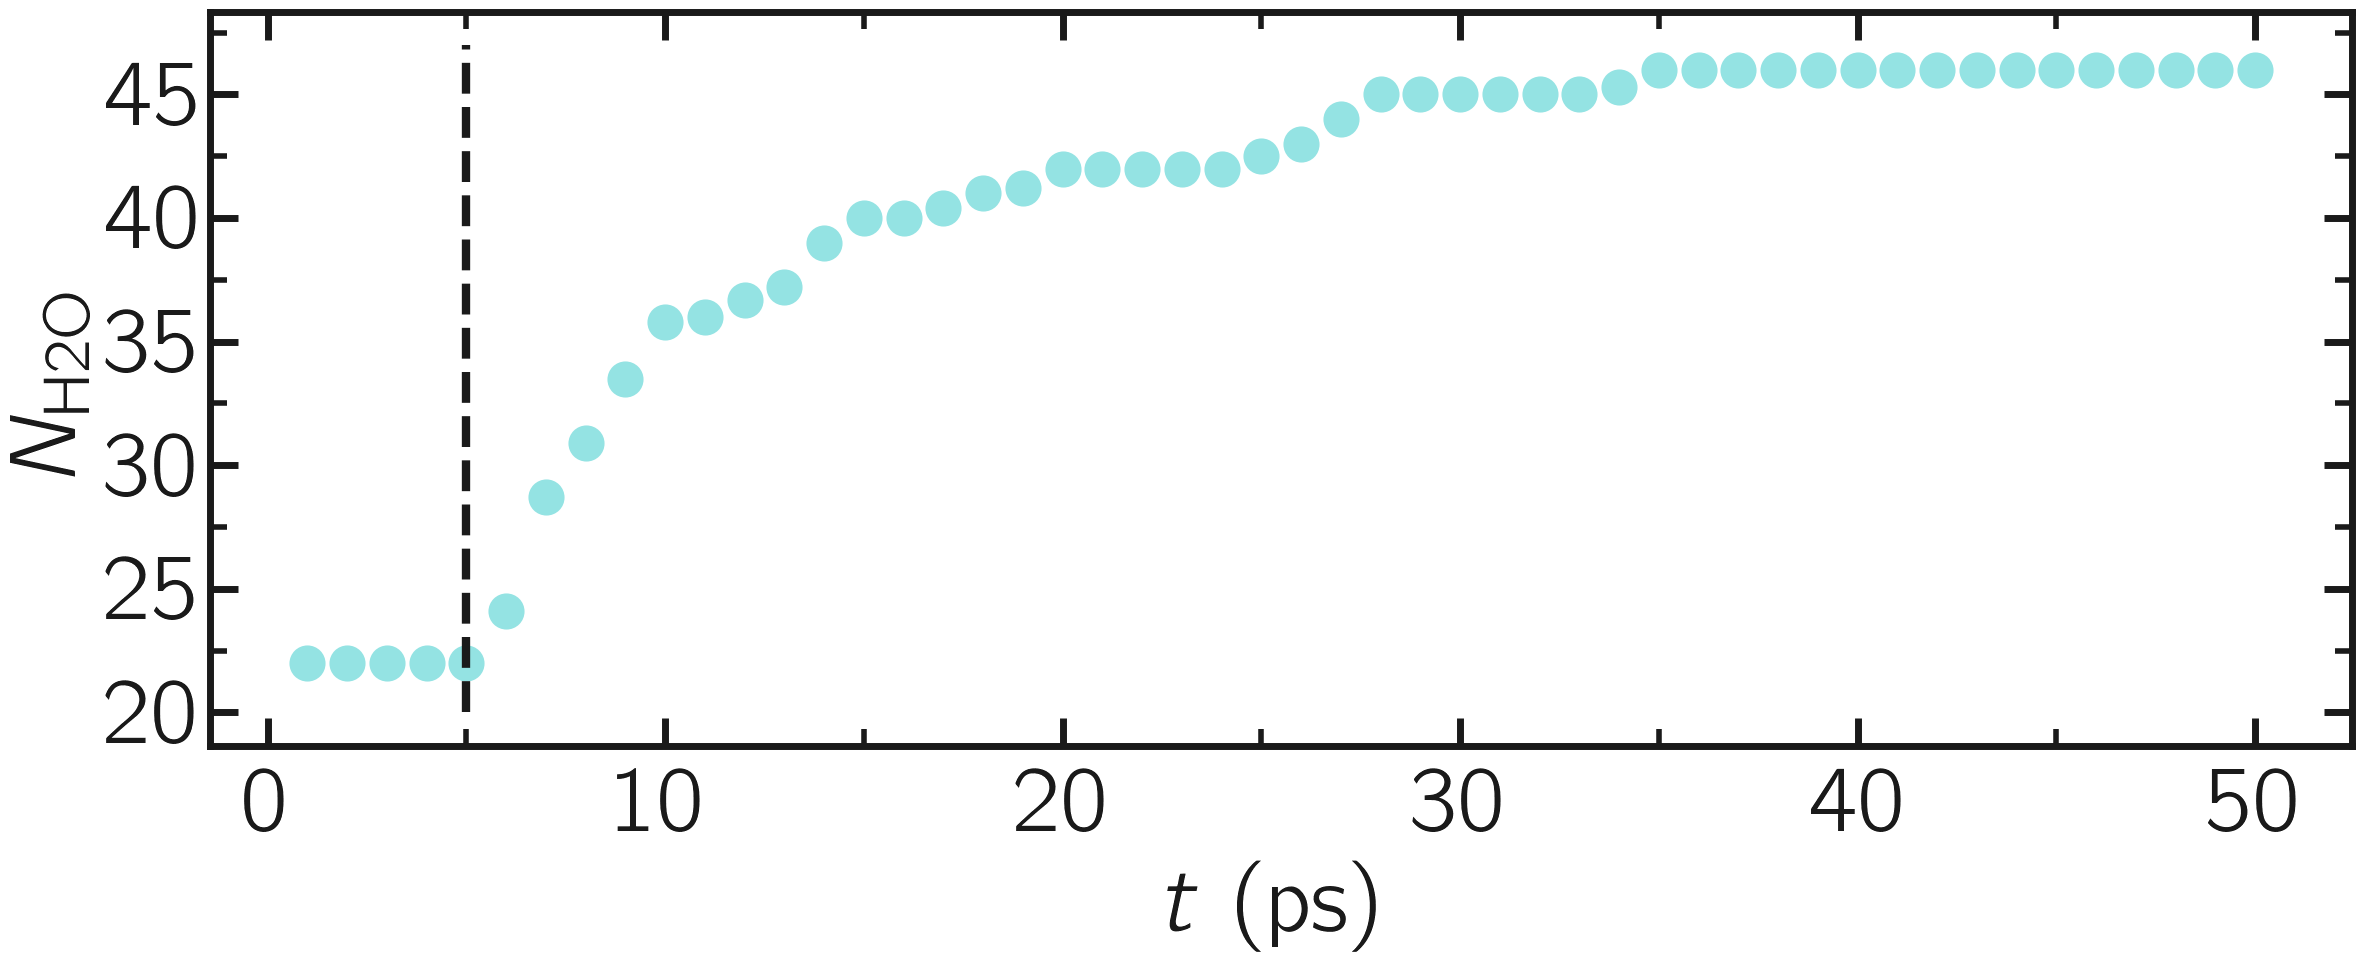
\includegraphics[width=\linewidth]{GCMC-number}
\caption{Number of water molecules $N_\text{H2O}$ as a function of the time $t$.
The dashed vertical line marks the beginning of the GCMC step.}
\label{fig:GCMC-number}
\end{figure}

When you run the simulation, the log file indicates that 840 atoms (i.e.~280 molecules)
were added by the \textit{create\_atoms} command (the exact number you get may differ):
\begin{lstlisting}
Created 840 atoms
\end{lstlisting}
You can also see that 258 molecules were immediately deleted, leaving 24 water
molecules (again, the exact number you get may differ):
\begin{lstlisting}
Deleted 774 atoms, new total = 642
Deleted 516 bonds, new total = 44
Deleted 258 angles, new total = 22
\end{lstlisting}
After just a few GCMC steps, the number of molecules starts increasing. Once the
crack is filled with water molecules, the number of molecules reaches a plateau
(Figs.\,\ref{fig:GCMC-number}-\ref{fig:GCMC-solvated}). The final number of
molecules depends on the imposed pressure, temperature, and the interaction
between water and silica (i.e.~its hydrophilicity). Note that GCMC simulations
of such dense phases are usually slow to converge due to the very low probability
of successfully inserting a molecule. Here, the short simulation duration was
made possible by the use of a large pressure.

\begin{figure}
\centering
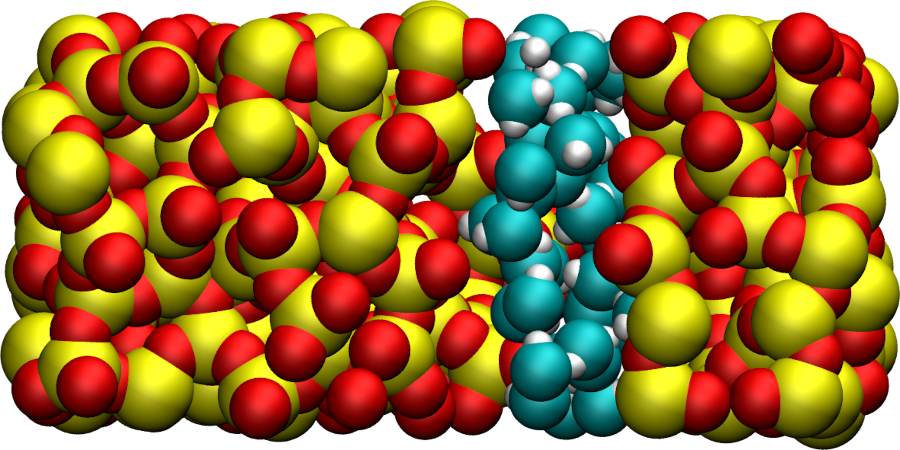
\includegraphics[width=\linewidth]{GCMC-solvated}
\caption{Snapshot of the silica system after the adsorption of water molecules.
The oxygen atoms of the water molecules are represented in cyan, the silicon
atoms in yellow, and the oxygen atoms of the solid in red.}
\label{fig:GCMC-solvated}
\end{figure}

\subsection{Tutorial 7: Free energy calculation}
\label{umbrella-sampling-label}

\begin{figure}
\centering
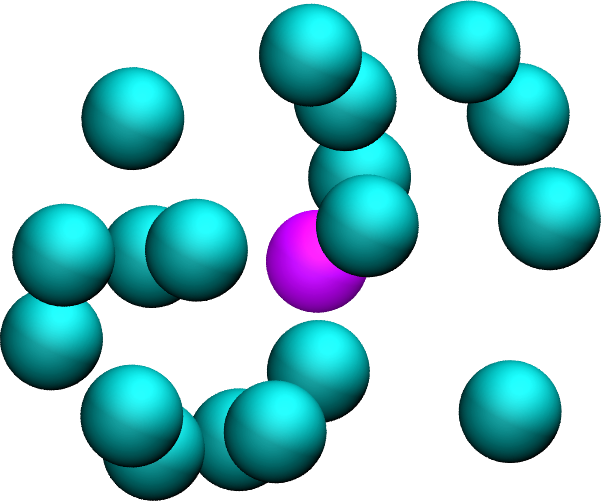
\includegraphics[width=0.55\linewidth]{US}
\caption{Atoms as simulated during \hyperref[umbrella-sampling-label]{Tutorial 7}.
Only the atom colored in pink feels the additional force used for the umbrella
sampling method.}
\label{fig:US}
\end{figure}

\noindent The objective of this tutorial is to measure the free energy profile
of particles across a barrier potential using two methods: free sampling and
umbrella sampling \cite{kastner2011umbrella, allen2017computer, frenkel2023understanding} (Fig.\,\ref{fig:US}).
For simplicity and to reduce computation time, the barrier potential will be
imposed on the atoms with an additional force, mimicking the presence of a repulsive
area in the middle of the simulation box without the need to simulate extra atoms.
The procedure is valid for more complex systems and can be adapted to many other
situations, such as measuring the adsorption barrier near an interface, or for
calculating a translocation barrier through a membrane
\cite{wilson1997adsorption, makarov2009computer, gravelle2021adsorption}.

\subsubsection{Method 1: Free sampling}
The most direct way to calculate a free energy profile is to extract the partition
function from a classical (i.e.~unbiased) molecular dynamics simulation, and
then estimate the Gibbs free energy using
\begin{equation}
\Delta G = -RT \ln(p/p_0),
\label{eq:G}
\end{equation}
where $\Delta G$ is the free energy difference, $R$ is the gas constant, $T$
is the temperature, $p$ is the pressure, and $p_0$ is a reference pressure.
As an illustration, let us apply this method to an extremely simple configuration
that consists of a few particles diffusing in a box in the presence of a
position-dependent repelling force that makes the center of the box a relatively
unfavorable area to explore.

\paragraph{Basic LAMMPS parameters}
\noindent Create a folder called \textit{FreeSampling/}, and create an input
script called \flecmd{input.lmp} in it. Copy the following lines into it:
\begin{lstlisting}
variable sigma equal 3.405
variable epsilon equal 0.238
variable U0 equal 1.5*${epsilon}
variable dlt equal 0.5
variable x0 equal 5.0

units real
atom_style atomic
pair_style lj/cut 3.822
pair_modify shift yes
boundary p p p
\end{lstlisting}
Here, we start by defining variables for the Lennard-Jones interaction
$\sigma$ and $\epsilon$ and for the repulsive potential $U$: $U_0$, $\delta$, and $x_0$,
see the analytical expression below. The value of 3.822 for the cut-off was chosen to
create a WCA, purely repulsive, potential \cite{weeks1971role}. It was calculated
as $2^{1/6} \times 3.405$ where $3.405 = \sigma$. The potential is shifted to be
equal to 0 at the cut-off using the \textit{pair\_modify}. The system of unit
\textit{real}, for which energy is in kcal/mol, distance in Ångstrom, or time in
femtosecond, has been chosen for practical reasons: the WHAM algorithm used in
the second part of the tutorial automatically assumes the energy to be in kcal/mol.

\paragraph{System creation and settings}
\noindent Let us define the simulation box and randomly add atoms by copying the
following lines into \flecmd{input.lmp}:
\begin{lstlisting}
region myreg block -25 25 -5 5 -25 25
create_box 1 myreg
labelmap atom 1 A1
create_atoms A1 random 60 34134 myreg &
    overlap 1.5 maxtry 50

mass * 39.95
pair_coeff * * ${epsilon} ${sigma}
neigh_modify every 1 delay 4 check yes
\end{lstlisting}

The variables $U_0$, $\delta$, and $x_0$ defined in the previous subsection are
used here to create the repulsive potential, restricting the atoms from exploring
the center of the box:
\begin{equation}
U = U_0 \left[ \arctan \left( \dfrac{x+x_0}{\delta} \right)
- \arctan \left(\dfrac{x-x_0}{\delta} \right) \right].
\label{eq:U}
\end{equation}
From the derivative of the potential with respect to $x$, we obtain the expression
for the force that will be imposed on the atoms:
\begin{equation}
F= \dfrac{U_0}{\delta} \left[ \dfrac{1}{(x-x_0)^2/\delta^2+1}
- \dfrac{1}{(x+x_0)^2/\delta^2+1} \right].
\label{eq:F}
\end{equation}
Fig.\,\ref{fig:potential} shows the potential $U$ and force $F$ along the $x$ axis.
With $U_0 = 1.5 \epsilon = 0.36\,\text{kcal/mol}$, $U_0$ is of the same order as the
thermal energy $k_\text{B} T = 0.24\,\text{kcal/mol}$, where $k_\text{B} = 0.002\,\text{kcal/mol/K}$
is the Boltzmann constant and $T = 119.8\,\text{K}$ (see below). In this case,
particles are expected to regularly overcome the energy barrier thanks to
the thermal agitation.

\begin{figure}
\centering
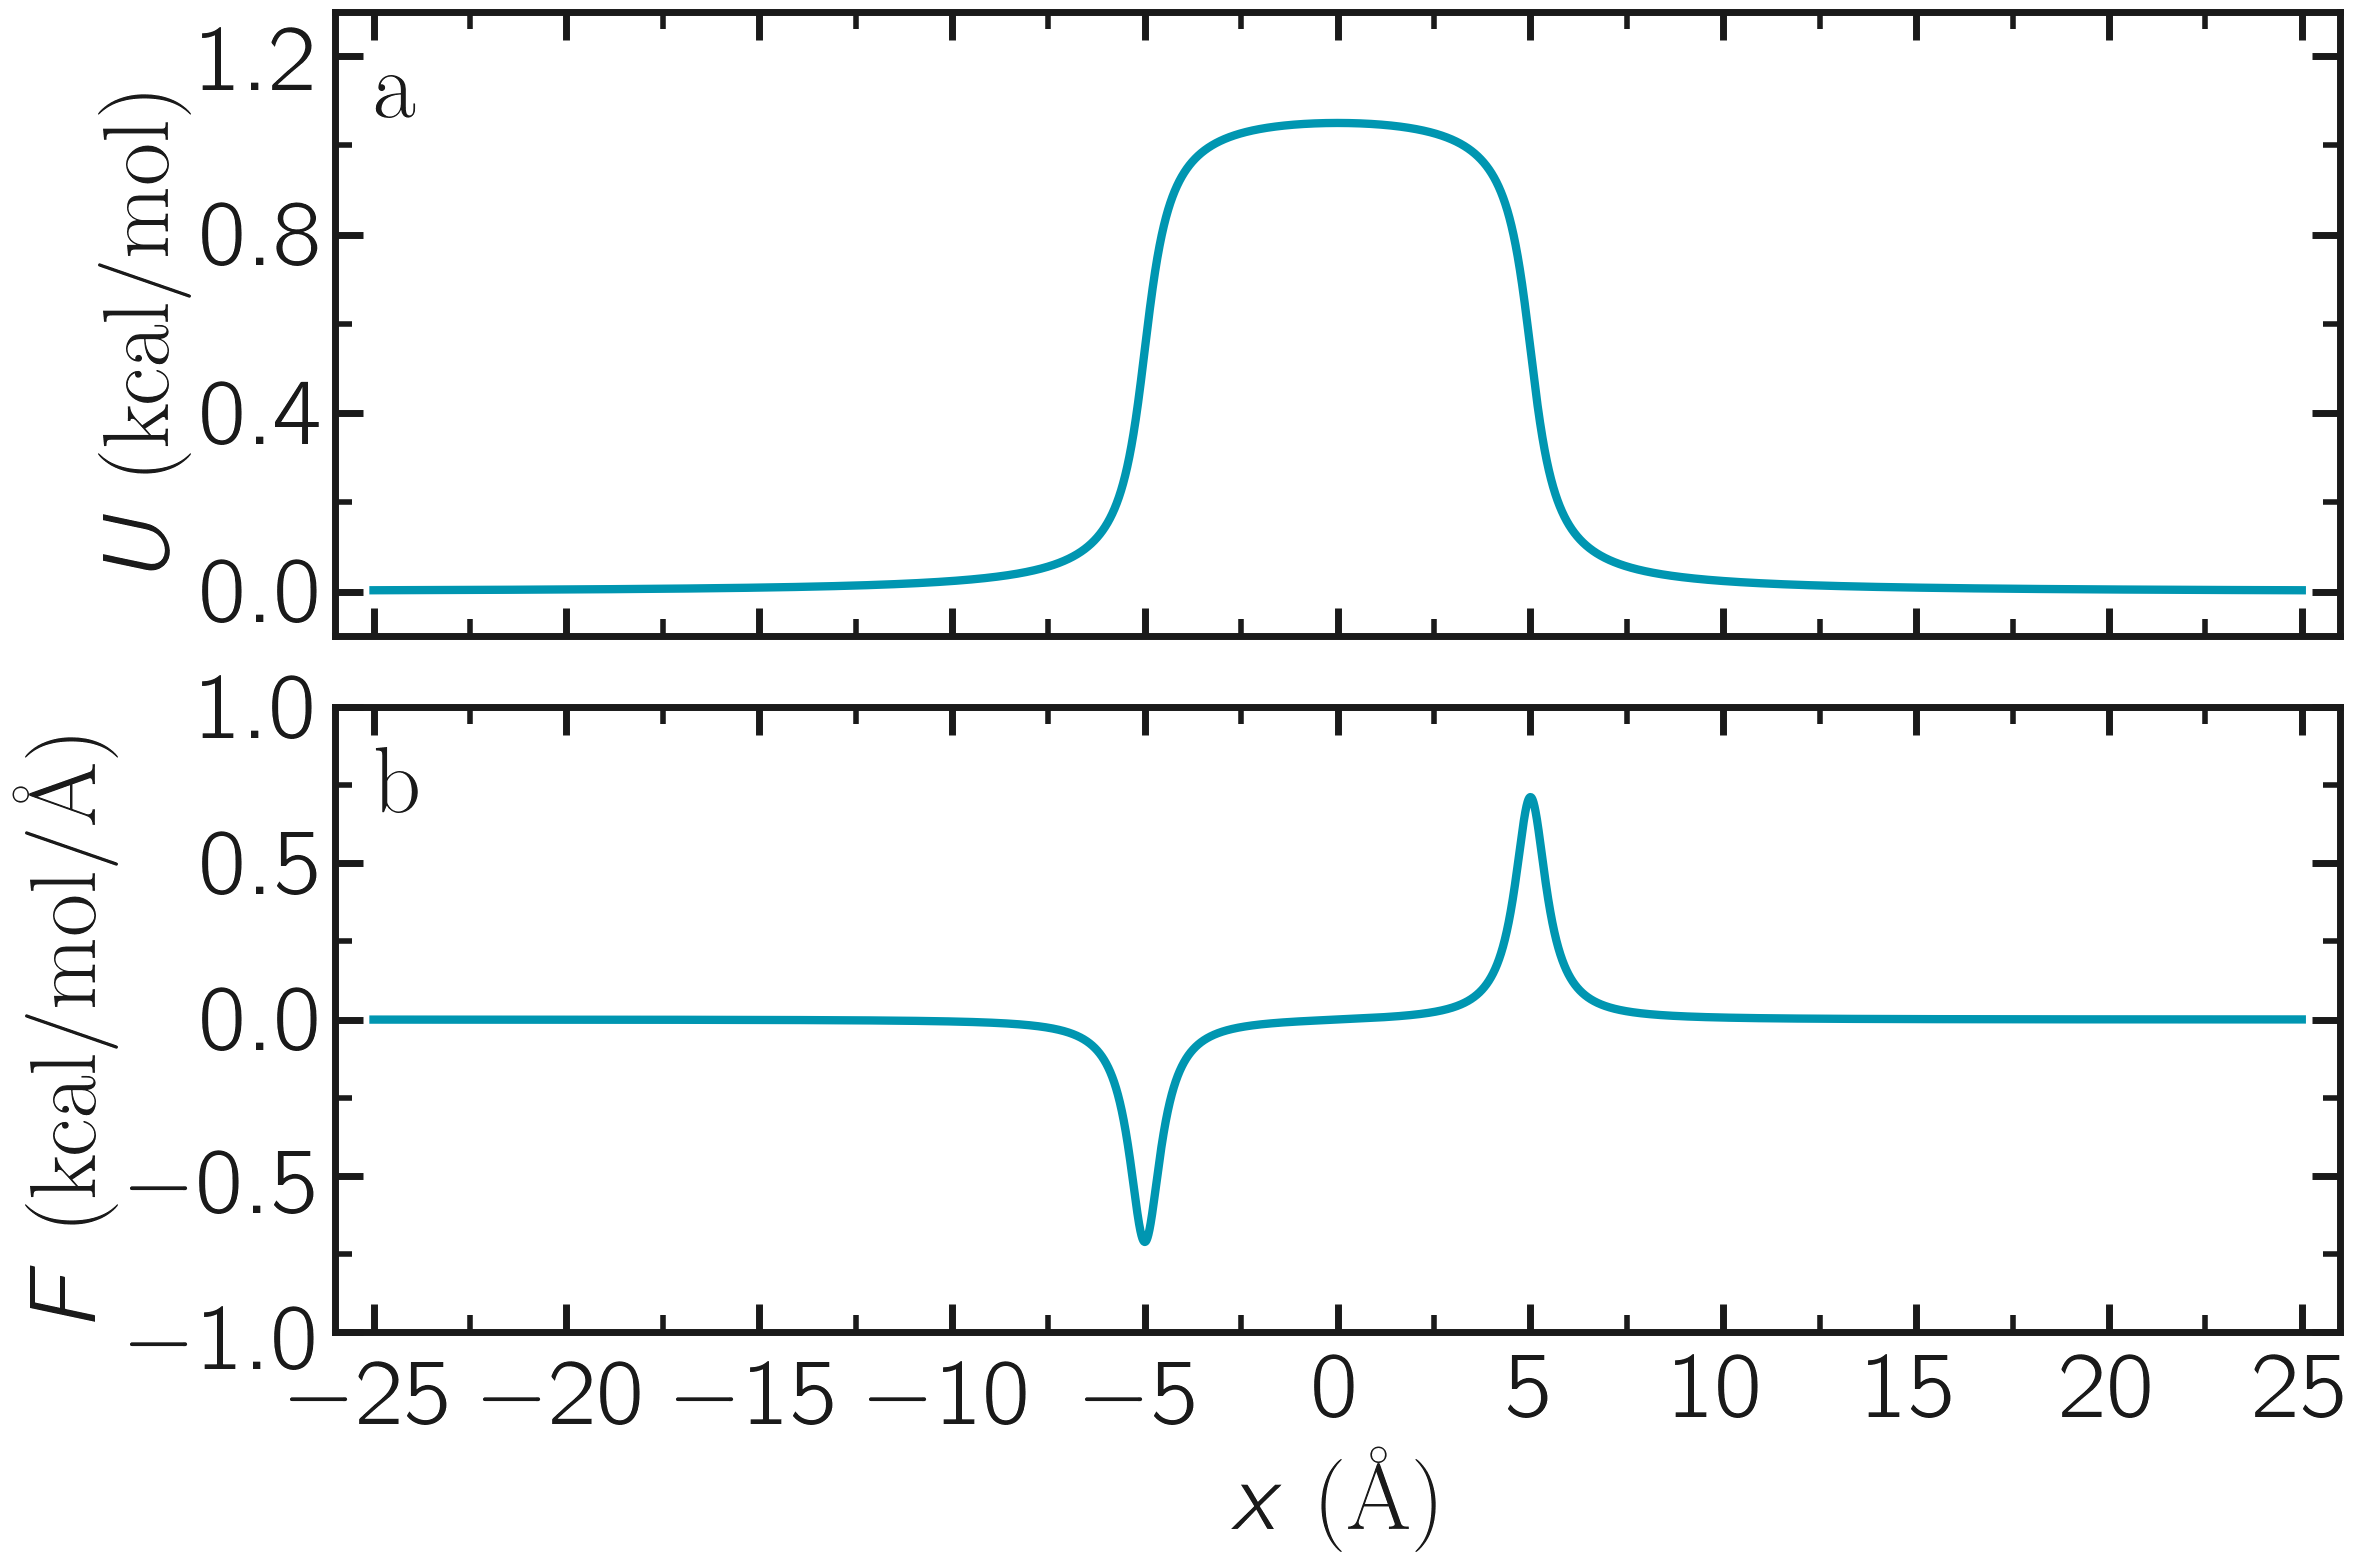
\includegraphics[width=\linewidth]{US-potential}
\caption{Potential $U$ given in Eq.\,\eqref{eq:U} (a) and force $F$ given in
Eq.\,\eqref{eq:F} (b) as a function of the coordinate $x$. Here,
$U_0 = 0.36~\text{kcal/mol}$, $\delta = 0.5~\mathrm{\AA{}}$, and $x_0 = 5~\mathrm{\AA{}}$.}
\label{fig:potential}
\end{figure}

Let us apply energy minimization to the system, and then impose the force $F(x)$
to all of the atoms in the simulation using the \textit{addforce} command. Add
the following lines to \flecmd{input.lmp}:
\begin{lstlisting}
minimize 1e-4 1e-6 100 1000
reset_timestep 0

variable U atom ${U0}*atan((x+${x0})/${dlt})&
    -${U0}*atan((x-${x0})/${dlt})
variable F atom &
    ${U0}/((x-${x0})^2/${dlt}^2+1)/${dlt}&
    -${U0}/((x+${x0})^2/${dlt}^2+1)/${dlt}
fix myadf all addforce v_F 0.0 0.0 energy v_U
\end{lstlisting}
Finally, let us combine the \textit{fix nve} with a \textit{Langevin} thermostat
and run a molecular dynamics simulation:
\begin{lstlisting}
fix mynve all nve
fix mylgv all langevin 119.8 119.8 50 1530917
\end{lstlisting}
With these two commands, the MD simulation
is effectively in the NVT ensemble: constant number of atoms $N$, constant volume
$V$, and constant temperature $T$.

To make sure that $1\,\text{ns}$ is long enough, we will record the evolution of
the number of atoms in the central (energetically unfavorable) region called \textit{mymes}
using the \textit{n\_center} variable:
\begin{lstlisting}
region mymes block -${x0} ${x0} INF INF INF INF
variable n_center equal count(all,mymes)
thermo_style custom step temp etotal v_n_center
thermo 10000

dump mydmp all image 5000 dump.*.jpg type type &
    shiny 0.1 box yes 0.02 view 0 90 zoom 1.9
dump_modify mydmp backcolor white &
    acolor A1 cyan adiam A1 1 boxcolor black
\end{lstlisting}
A \textit{dump image} was also added for system visualization.

Finally, let us perform an equilibration of 500000 steps
in total, using a timestep of $2\,\text{fs}$ (i.e.~a total duration of $1\,\text{ns}$):
\begin{lstlisting}
timestep 2.0
run 500000
\end{lstlisting}
Run the simulation with LAMMPS. To ensure that the equilibration of $1\,\text{ns}$ is long
enough, let us have a look at the evolution of the number of atoms in the central region,
$n_\mathrm{center}$. We can see that $n_\mathrm{center}$ reaches
its equilibrium value (which is close to 0) after about $0.1\,\text{ns}$
(Fig.\,\ref{fig:US-density-evolution}). See also a snapshot of the equilibrated
system in Fig.\,\ref{fig:US-system-unbiased}.

\paragraph{Run and data acquisition}
Once the system is equilibrated, let us record the density profile of
the atoms along the $x$ axis using
the \textit{ave/chunk} command. A total of 10 density profiles will be printed.
Add the following line to \flecmd{input.lmp}:
\begin{lstlisting}
unfix myat
undump mydmp
reset_timestep 0

compute cc1 all chunk/atom bin/1d x 0.0 1.0
fix myac all ave/chunk 10 400000 4000000 &
    cc1 density/number file density_profile.dat
dump mydmp all atom 200000 dump.lammpstrj

thermo 100000
run 4000000
\end{lstlisting}
The step count is reset to 0 using \textit{reset\_timestep} to synchronize
with the output times of \textit{fix density/number}. Feel free to increase the
duration of the last run for a better resolved density profile.

\begin{figure}
\centering
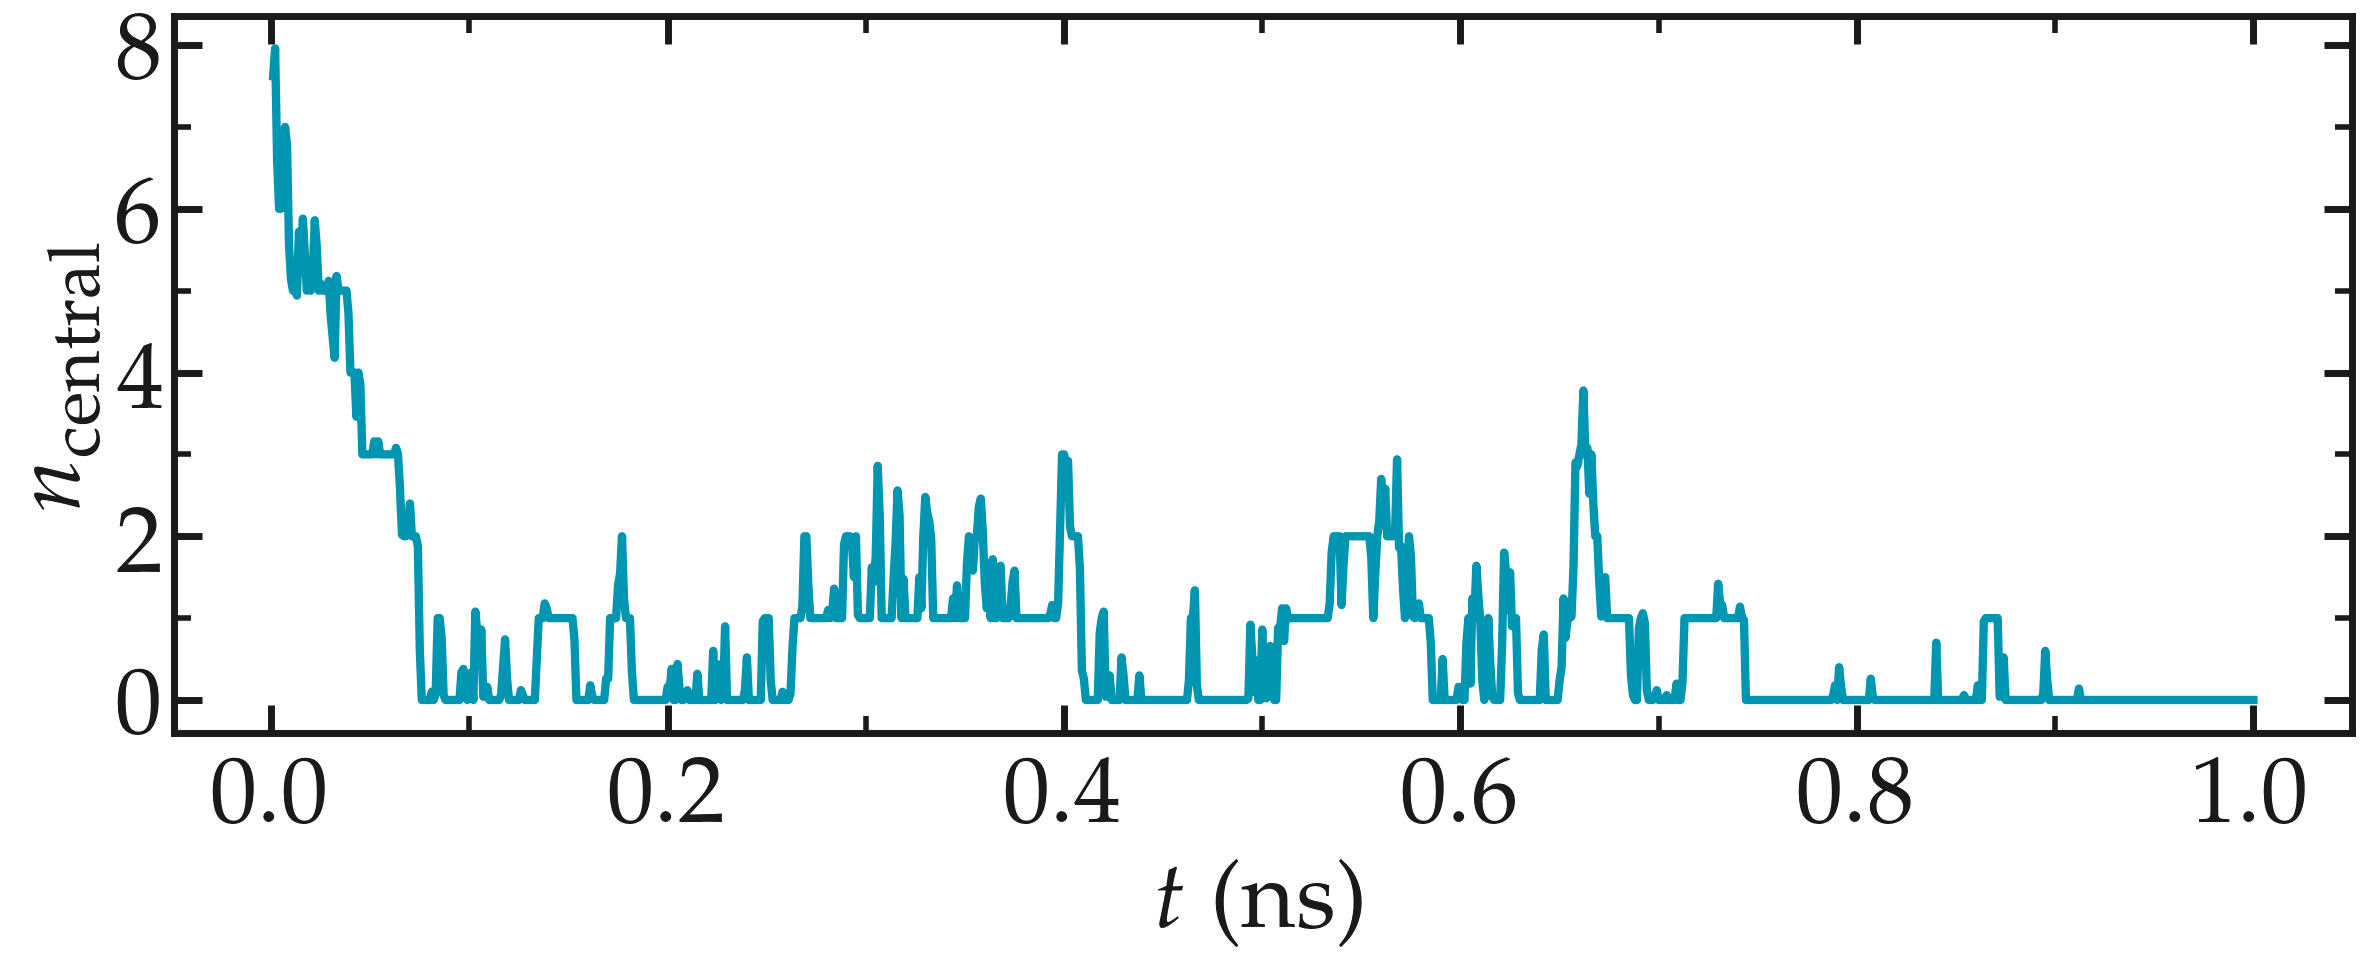
\includegraphics[width=\linewidth]{US-density-evolution}
\caption{Evolution of the number of atoms $n_\text{center}$ in the central
region \textit{mymes} as a function of time $t$ during equilibration. The dark line
serves as a guide for the eyes. Here, $U_0 = 0.36~\text{kcal/mol}$,
$\delta = 0.5~\mathrm{\AA{}}$, and $x_0 = 5~\mathrm{\AA{}}$.}
\label{fig:US-density-evolution}
\end{figure}

\paragraph{Data analysis}

Once the simulation is over, the density profile shows that the density in the center of the box is
about two orders of magnitude lower than inside the reservoir (Fig.\,\ref{fig:US-density}).
Then, let us plot $-R T \ln(\rho/\rho_\mathrm{bulk})$ (i.e.~Eq.\,\eqref{eq:G} where
the pressure ratio $p/p_\mathrm{bulk}$ is replaced by the density ratio
$\rho/\rho_\mathrm{bulk}$ assuming the system is an ideal gas) and compare it
with the imposed potential $U$ from Eq.\,\eqref{eq:U} (Fig.\,\ref{fig:US-FreeSampling}).
The value for the reference density $\rho_\text{bulk} = 0.0033~\text{\AA{}}^{-3}$
was estimated by measuring the density of the reservoir from the raw density
profiles. The agreement between the MD results and the imposed energy profile
is reasonable, despite some noise in the central part (where fewer data points
are available due to the repulsive potential).

\begin{figure}
\centering
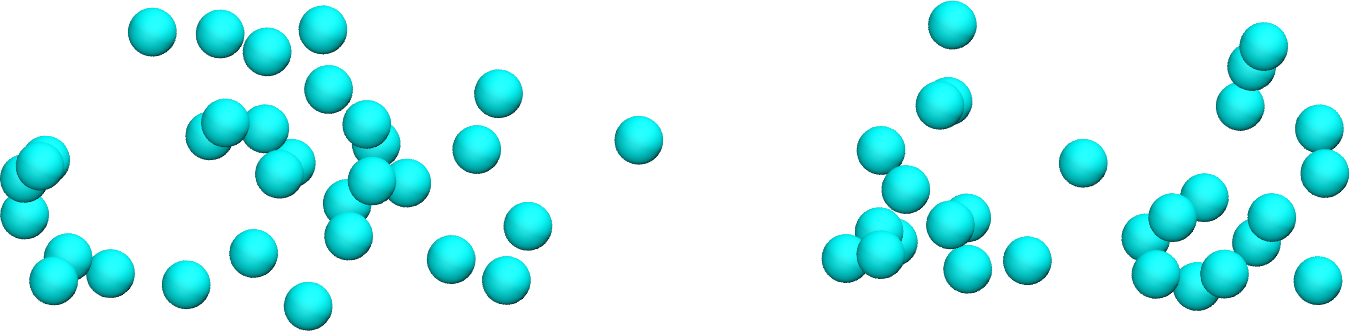
\includegraphics[width=\linewidth]{US-system-unbiased}
\caption{Snapshot of the system. The density of atoms is lowest in the central
part of the box, \textit{mymes}, due to the additional force $F$. Here,
$U_0 = 0.36~\text{kcal/mol}$, $\delta = 0.5~\mathrm{\AA{}}$, and $x_0 = 5~\mathrm{\AA{}}$.}
\label{fig:US-system-unbiased}
\end{figure}

\begin{figure}
\centering
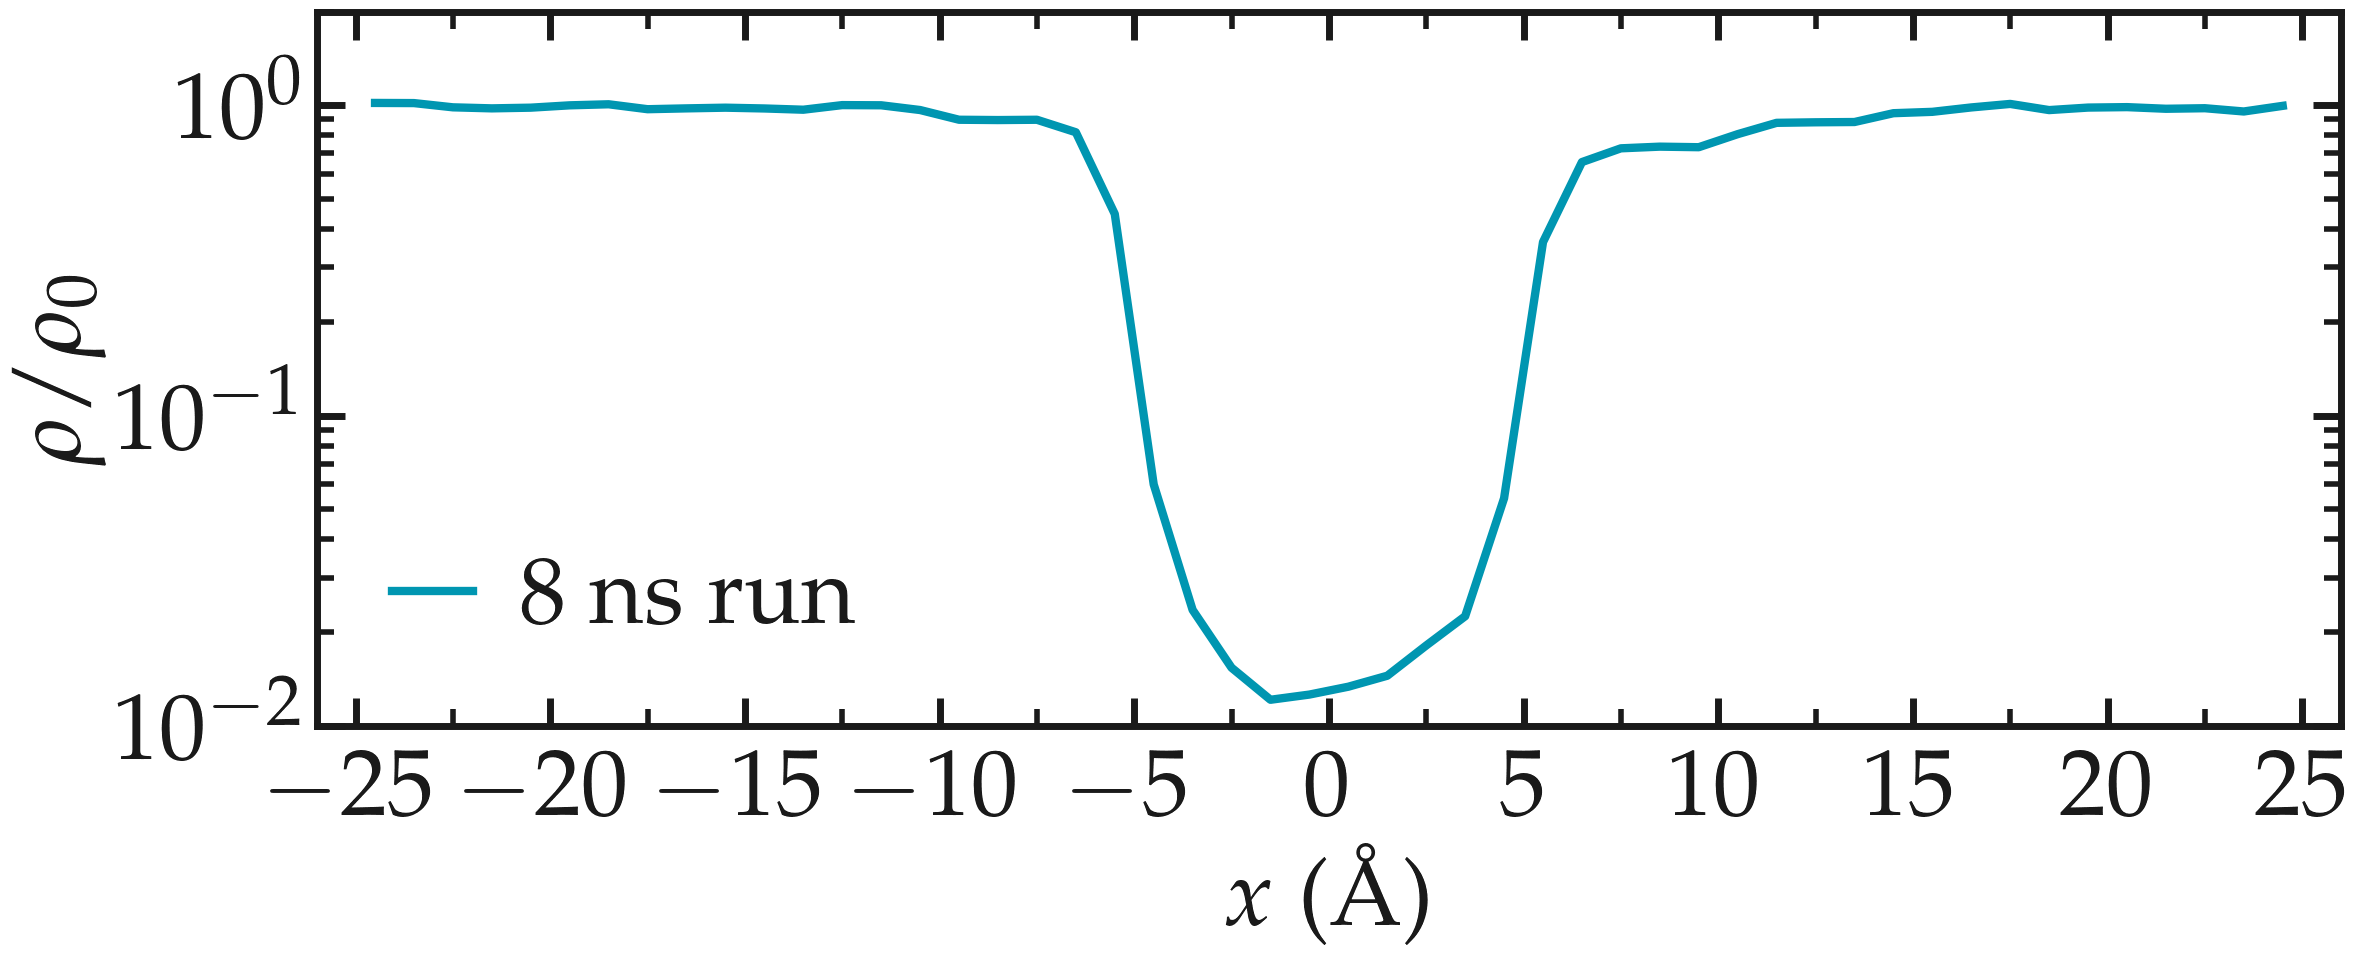
\includegraphics[width=\linewidth]{US-density}
\caption{Fluid density $\rho$ along the $x$ direction. Here,
$U_0 = 0.36~\text{kcal/mol}$, $\delta = 0.5~\mathrm{\AA{}}$, $x_0 = 5~\mathrm{\AA{}}$,
and reference density $\rho_\text{bulk} = 0.0033~\text{\AA{}}^{-3}$.}
\label{fig:US-density}
\end{figure}

\begin{figure}
\centering
\includegraphics[width=\linewidth]{US-FreeSampling}
\caption{Potential $U$ as a function of $x$ measured using free sampling (blue disks)
compared to the imposed potential given in Eq.\,\eqref{eq:U} (dark line). Here,
$U_0 = 0.36~\text{kcal/mol}$, $\delta = 0.5~\mathrm{\AA{}}$, and $x_0 = 5~\mathrm{\AA{}}$.}
\label{fig:US-FreeSampling}
\end{figure}

\paragraph{The limits of free sampling}
If we increase the value of $U_0$, the average number of atoms in the central
region will decrease, making it difficult to obtain a good resolution for the free
energy profile. For instance, when we run the same simulation using $U_0 = 10 \epsilon$,
which corresponds to a situation where $U_0 \approx 10 k_\text{B} T$, not a single
atom explores the central part of the simulation box during the 8 ns of simulation.
In this case, using an enhanced sampling method is preferred; see the next section.

\subsubsection{Method 2: Umbrella sampling}
Umbrella sampling is a biased molecular dynamics method in which additional forces
are added to a chosen atom to force it to explore the more unfavorable areas of
the system \cite{kastner2011umbrella, allen2017computer, frenkel2023understanding}.
Here, to encourage one of the atoms to explore the central region of the box,
we apply a potential $V$ and force it to move along the $x$-axis. The chosen path
is called the axis of reaction. Several simulations (called windows) will be
conducted with varying positions for the center of the applied biasing. The results
will be analyzed using the weighted histogram analysis method (WHAM) \cite{kumar1992weighted},
which allows for the removal of the biasing effect and ultimately deduces the
unbiased free energy profile.

\paragraph{LAMMPS input script}
Create a new folder called \flrcmd{BiasedSampling/}, and create a new input file
called \flecmd{input.lmp} in it, and copy the following lines:
\begin{lstlisting}
variable sigma equal 3.405
variable epsilon equal 0.238
variable U0 equal 10*${epsilon}
variable dlt equal 0.5
variable x0 equal 5.0
variable k equal 1.5

units real
atom_style atomic
pair_style lj/cut 3.822
pair_modify shift yes
boundary p p p

region myreg block -25 25 -5 5 -25 25
create_box 2 myreg
labelmap atom 1 A1 2 A2
create_atoms A2 single 0 0 0
create_atoms A1 random 5 34134 myreg &
    overlap 1.5 maxtry 50

mass * 39.948
pair_coeff * * ${epsilon} ${sigma}
neigh_modify every 1 delay 4 check yes
group topull type 2

minimize 1e-4 1e-6 100 1000
reset_timestep 0

variable U atom ${U0}*atan((x+${x0})/${dlt})&
    -${U0}*atan((x-${x0})/${dlt})
variable F atom &
    ${U0}/((x-${x0})^2/${dlt}^2+1)/${dlt}&
    -${U0}/((x+${x0})^2/${dlt}^2+1)/${dlt}
fix pot all addforce v_F 0.0 0.0 energy v_U

fix mynve all nve
fix mylgv all langevin 119.8 119.8 50 1530917
timestep 2.0
thermo 100000
run 500000
reset_timestep 0

dump mydmp all image 1000000 dump.*.jpg type &
type shiny 0.1 box yes 0.02 view 0 90 zoom 1.9
dump_modify mydmp backcolor white &
    acolor A1 cyan adiam A1 1 &
    acolor A2 pink adiam A2 1 &
    boxcolor black
\end{lstlisting}
So far, this code resembles that of Method 1, except for the additional particle
of type A2. Particles of type A1 and A2
are identical, having the same mass and Lennard-Jones parameters. However, the
particle of type A2 will additionally be exposed to the biasing potential
$V$ (Fig.\,){fig:US-system-biased}).

Let us create a loop with 50 steps, and move progressively the center of the
bias potential by an increment of 0.1 nm. Add the following lines to \flecmd{input.lmp}:
\begin{lstlisting}
variable a loop 50
label loop
variable xdes equal ${a}-25
variable xave equal xcm(topull,x)
fix mytth topull spring tether ${k} &
    ${xdes} 0 0 0
run 200000
fix myat1 all ave/time 10 10 100 v_xave &
    v_xdes file data/position.${a}.dat
run 1000000
unfix myat1
next a
jump SELF loop
\end{lstlisting}
A folder called \flrcmd{data/} needs to be created within \flrcmd{BiasedSampling/}.
The spring command serves to impose the additional harmonic potential $V$ with
the spring constant $k$. Note that the value of $k$ should be chosen with care,
if $k$ is too small, the particle won't follow the biasing potential center,
and if $k$ is too large, there will be no overlapping between the different windows.
The center of the harmonic potential $x_\text{des}$ successively takes values
from -25 to 25. For each value of $x_\text{des}$, an equilibration step of 0.4 ns
is performed, followed by a step of 2 ns during which the position along $x$ of
the particle is saved in data files (one data file per value of $x_\text{des}$).
You can always increase the duration of the runs for better samplings. Run the
\flecmd{input.lmp}  file using LAMMPS.

\begin{figure}
\centering
\includegraphics[width=\linewidth]{US-system-biased}
\caption{Snapshot of the system with atoms of type 1 in cyan and the single atom
of type 2 in pink. Only the atom of type 2 explores the central part of the box,
\textit{mymes}, due to its additional biasing potential $V$. Here,
$U_0 = 2.38~\text{kcal/mol}$, $\delta = 0.5~\mathrm{\AA{}}$, and $x_0 = 5~\mathrm{\AA{}}$.}
\label{fig:US-system-biased}
\end{figure}

\paragraph{WHAM algorithm}
\noindent To generate the free energy profile from the density distribution,
let us use the WHAM algorithm as implemented by Marc Grossfield \cite{grossfieldimplementation}.
You can download it from \href{http://membrane.urmc.rochester.edu/?page_id=126}{Alan Grossfield}
website, and compile it by typing in the terminal:
\begin{lstlisting}
cd wham
make clean
make
\end{lstlisting}
\noindent The compilation creates an executable called \textit{wham} that you can
copy in the \flrcmd{BiasedSampling/} folder. To apply the WHAM algorithm to our
simulation, we first need to create a metadata file. This file simply contains
\begin{itemize}
\item the paths to all the data files,
\item the value of $x_\text{des}$,
\item and the values of $k$.
\end{itemize}
Download the \href{\filepath tutorial7/metadata.dat}{\dwlcmd{metadata.dat}}
file I have written and save it in \flrcmd{BiasedSampling/}. Then, simply run the
following command in the terminal:
\begin{lstlisting}
./wham -25 25 50 1e-8 119.8 0 \
    metadata.dat PMF.dat
\end{lstlisting}
where -25 and 25 are the boundaries, 50 is the number of bins, 1e-8 is the tolerance,
and 119.8 is the temperature. A file called \textit{PMF.dat} has been created,
containing the free energy profile in kcal/mol. Again, one can compare the result of
the PMF with the imposed potential $U$, demonstrating excellent agreement
(Fig.\,\ref{fig:US-freenergy}). We can see that the agreement is quite good despite
the very short calculation time and the very high value for the energy barrier.
Obtaining the same results with Free Sampling would require performing extremely
long and costly simulations.

\begin{figure}
\centering
\includegraphics[width=\linewidth]{US-freenergy}
\caption{Potential $U$ as a function of $x$ measured using umbrella sampling
(blue disks) compared to the imposed potential given in Eq.\,\eqref{eq:U}
(dark line). Here, $U_0 = 2.38~\text{kcal/mol}$, $\delta = 0.5~\mathrm{\AA{}}$,
and $x_0 = 5~\mathrm{\AA{}}$.}
\label{fig:US-freenergy}
\end{figure}

\subsection{Tutorial 8: Reactive Molecular Dynamics}
\label{bond-react-label}

\begin{figure}
\centering
\includegraphics[width=0.55\linewidth]{REACT}
\caption{Polymer melt made in nylon and carbon nanotubes (CNTs) simulated during
\hyperref[bond-react-label]{Tutorial 8}. The water molecules (in red and white)
are created by the polymerization of nylon simulation using REACTER.}
\label{fig:REACT}
\end{figure}

The goal of this tutorial is to create a system made of 
carbon nanotubes (CNTs) embedded in a polymer melt made in nylon-6,6 (Fig.\,\ref{fig:REACT}). The
REACTER protocol is used to simulate the polymerization of nylon, and the formation
of water molecules is followed in time \cite{gissinger2020reacter, gissinger2024molecular}.
In contrast with Airebo (\hyperref[carbon-nanotube-label]{Tutorial 2})
and ReaxFF (\hyperref[reactive-silicon-dioxide-label]{Tutorial 5}), the REACTER
protocol relies on the use of a \textit{classical} force field.

\subsubsection{Creating the system}

The first step of the tutorial is to mix small carbon nanotubes
with the initial, unreacted, molecules. The molecules are hexamethylenediamine
(C$_6$H$_{16}$N$_2$) and adipic acid (C$_6$H$_{10}$O$_4$). Create a new input
file, call it \textit{mixing.lmp}, and copy the following lines into it:
{\normalsize
\begin{verbatim}
units real
boundary p p p
atom_style full

kspace_style pppm 1.0e-5
pair_style lj/class2/coul/long 8.5
angle_style class2
bond_style class2
dihedral_style class2
improper_style class2
pair_modify tail yes mix sixthpower
special_bonds lj/coul 0 0 1
\end{verbatim}
}
The \textit{class2} styles compute a 6/9 Lennard-Jones \cite{sun1998compass}.
The \textit{class2} bonds, angles, dihedrals, and impropers are used as
well, see the documention for a description of their respective potentials.
The \textit{mix sixthpower} imposes the following mixing rule for the calculation
of the cross coefficients: $\sigma_{ij} = ( 0.5 (\sigma^6_i+\sigma_j^6))^{1/6}$,
and $\epsilon_{ij} = (2 \sqrt{\epsilon_i \epsilon_j} \sigma^3_i \sigma^3_j)
/ (\sigma^6_i+\sigma_j^6)$.

Let us read a data file named \href{\filepath tutorial8/nylon.data}{\textit{nylon.data}}
containing the unreacted molecule template, and let us replicate it. Add the
folloxing lines to \textit{mixing.lmp}:
{\normalsize
\begin{verbatim}
read_data nylon.data &
  extra/bond/per/atom 5  &
  extra/angle/per/atom 15 &
  extra/dihedral/per/atom 15 &
  extra/improper/per/atom 25 &
  extra/special/per/atom 25
replicate 3 4 4
\end{verbatim}
}
The resulting box is $(7.2\,\text{nm})^3$ in size, and its density is low
enough that inserting CNTs will be easy.
% S.G.: @jrgissing, here we could describe the content of nylon.data.
% How was it created, what is the specifity of the molecules involved, etc...

To add 5 CNTs to the simulation box, add the following commands
to \textit{mixing.lmp}:
{\normalsize
\begin{verbatim}
molecule CNT cnt.molecule
create_atoms 0 random 5 8305 NULL overlap 3 &
  maxtry 500 mol CNT 7687
\end{verbatim}
}
Let us use the \textit{minimize} command to reduce the energy of the system:
{\normalsize
\begin{verbatim}
minimize 1.0e-4 1.0e-6 100 1000
reset_timestep 0
\end{verbatim}
}
Then, let us use \textit{dump image} to output images every 1000 steps:
{\normalsize
\begin{verbatim}
dump mydmp all image 1000 dump.mixing.*.ppm &
  type type shiny 0.1 box no 0.01 &
  view 0 0 zoom 1.8 fsaa yes bond atom 0.5
dump_modify mydmp backcolor white &
  acolor c2 gray acolor c_1 lightslategray &
  acolor o dimgray acolor o_1 dimgray &
  acolor hc lightslategray &
  acolor ho lightslategray &
  acolor hn lightslategray acolor hw white &
  acolor o* red acolor n darkslategray &
  acolor na darkslategray &
  acolor cp lightpink &
  adiam c2 0.3 adiam c_1 0.3 &
  adiam cp 0.3 adiam o 0.28 &
  adiam o_1 0.28 adiam o* 2.8 &
  adiam hc 0.15 adiam ho 0.15 &
  adiam hn 0.15 adiam hw 1.5 &
  adiam n 0.3 adiam na 0.3 
\end{verbatim}
}
Then, let us perform a short equilibration of system using \textit{fix npt}
with a isotropic couplage. To speed up the equilibration of the system, let us 
impose a relatively large pressure of 1000\,atm for the first 10\,ps:
{\normalsize
\begin{verbatim}
velocity all create 300 1829 dist gaussian &
  mom yes rot yes
fix mynpt all npt temp 300 300 100 &
  iso 1000 1000 1000

thermo 1000
thermo_style custom step temp pe etotal press &
  density vol

run 10000
\end{verbatim}
}
Then, for the following 20\,ps, let us continue the equilibration
with an imposed pressure of 1\,atm, and write the final state of the
system in a file named \textit{cnt-nylon-mix.data}:
{\normalsize
\begin{verbatim}
fix mynpt all npt temp 300 300 100 iso 1 1 1000

run 20000
write_data cnt-nylon-mix.data
\end{verbatim}
}
As the time progresses, the density $\rho$ of the system progressively
converges toward an equilibrium value $\rho \approx 1.3$\,g/cm$^3$
(Fig.\,\ref{fig:evolution-density}).

\begin{figure}
\centering
\includegraphics[width=\linewidth]{REACT-mixing}
\caption{Evolution of the system density, $\rho$, as a function of the
time, $t$, during equilibration.}
\label{fig:evolution-density}
\end{figure}

\subsubsection{Atom maps and molecule templates}

The REACTER protocol relies on classical force fields. For the reaction to
occur, an \textit{atom map} containing information about the reaction mechanism
must be provided by the user. The atom map specifies which atoms are
the initiators to the reaction and what are the distance cutoffs. In addition,
pre-reaction and post-reaction molecule templates must be provided.

Download the two atoms maps, \href{\filepath tutorial8/rxn1_stp1_map}{\textit{rxn1$\_$stp1$\_$map}}
and \href{\filepath tutorial8/rxn1_stp1_map}{\textit{rxn1$\_$stp1$\_$map}},
the two templates for the unreacted molecules,
\href{\filepath tutorial8/rxn1_stp1_unreacted.molecule_template}{\textit{rxn1$\_$stp1$\_$unreacted.molecule$\_$template}}
and 
\href{\filepath tutorial8/rxn1_stp2_unreacted.molecule_template}{\textit{rxn1$\_$stp2$\_$unreacted.molecule$\_$template}},
as well as the two templates for the reacted molecules,
\href{\filepath tutorial8/rxn1_stp1_reacted.molecule_template}{\textit{rxn1$\_$stp1$\_$reacted.molecule$\_$template}}
and 
\href{\filepath tutorial8/rxn1_stp2_reacted.molecule_template}{\textit{rxn1$\_$stp2$\_$reacted.molecule$\_$template}}.

% S.G.: @jrgissing, here we could describe the specifity, or at least the most important
% details of the atom maps.
% S.G.: the name of the molecule templates are too long. Would it be possible to shorten them
% for the sake of the tutorial? like "reacted-1.mol" instead of rxn1_stp1_reacted.molecule_template.

\subsubsection{Simulating the reaction}

The first step, before simulating the reaction, is to import the previously
generated configuration. Create a new input file named \textit{reacting.lmp},
and copy the following lines into it:
{\normalsize
\begin{verbatim}
units real
boundary p p p
atom_style full

kspace_style pppm 1.0e-5
pair_style lj/class2/coul/long 8.5
angle_style class2
bond_style class2
dihedral_style class2
improper_style class2
pair_modify tail yes mix sixthpower

special_bonds lj/coul 0 0 1

read_data cnt-nylon-mix.data &
  extra/bond/per/atom 5  &
  extra/angle/per/atom 15 &
  extra/dihedral/per/atom 15 &
  extra/improper/per/atom 25 &
  extra/special/per/atom 25
\end{verbatim}
}
Here, the \textit{read$\_$data} command is used to import \textit{cnt-nylon-mix.data}.
Then, let us import all four molecules template using the \textit{molecule} command:
{\normalsize
\begin{verbatim}
molecule mol1 rxn1_stp1_unreacted.molecule_template
molecule mol2 rxn1_stp1_reacted.molecule_template
molecule mol3 rxn1_stp2_unreacted.molecule_template
molecule mol4 rxn1_stp2_reacted.molecule_template 
\end{verbatim}
}
In order to follow the evolution of the reaction with time, let us generate images
of the system using \textit{dump image}:
{\normalsize
\begin{verbatim}
dump mydmp all image 1000 dump.mixing.*.ppm &
  type type shiny 0.1 box no 0.01 &
  view 0 0 zoom 1.8 fsaa yes bond atom 0.5
dump_modify mydmp backcolor white &
  acolor c2 gray acolor c_1 lightslategray &
  acolor o dimgray acolor o_1 dimgray &
  acolor hc lightslategray &
  acolor ho lightslategray &
  acolor hn lightslategray acolor hw white &
  acolor o* red acolor n darkslategray &
  acolor na darkslategray &
  acolor cp lightpink &
  adiam c2 0.3 adiam c_1 0.3 &
  adiam cp 0.3 adiam o 0.28 &
  adiam o_1 0.28 adiam o* 2.8 &
  adiam hc 0.15 adiam ho 0.15 &
  adiam hn 0.15 adiam hw 1.5 &
  adiam n 0.3 adiam na 0.3
\end{verbatim}
}
Then, using the \textit{fix bond/react}, 
{\normalsize
\begin{verbatim}
fix myrxns all bond/react &
  stabilization yes statted_grp 0.03 &
  react rxn1 all 1 0.0 2.9 mol1 mol2 rxn1_stp1_map 
  react rxn2 all 1 0.0 5.0 mol3 mol4 rxn1_stp2_map
\end{verbatim}
}
With the \textit{stabilization} keyword, the \textit{bond/react} command will
try to stabilize the atoms involved in the reaction using the nve/limit
command with a maximum displacement of $0.03\,\mathrm{\AA{}}$ (a command that was
used, for instance, in \hyperref[sheared-confined-label]{Tutorial 4}). The two
\textit{react} keywords contain specific details about the two reactions
involved here, i.e. a transformation of \textit{mol1} into \textit{mol2} based
on the atom map \textit{rxn1$\_$stp1$\_$map}, and a transformation of 
\textit{mol3} into \textit{mol4} based on the atom map \textit{rxn1$\_$stp2$\_$map}.

Finally, let us use the \textit{fix nvt} to perform the integration of the 
equation of motion and control the temperature of the system:
{\normalsize
\begin{verbatim}
fix mynvt statted_grp_REACT nvt $
  temp 300 300 100

thermo 1000
thermo_style custom step temp pe $
  etotal press f_myrxns[1] f_myrxns[2]

run 50000
\end{verbatim}
}
Here, in addition, the \textit{thermo custom} command was called and was
asked to print the cumulative reaction counts from \textit{fix myrxns}.
The number of reaction, $N_r$, can be seen to increase with time
(Fig.\,\ref{fig:evolution-reacting})

\begin{figure}
\centering
\includegraphics[width=\linewidth]{REACT-reacting}
\caption{Evolution of the reaction counts, $\text{N}_r$,
as a function of the time, $t$, during the reaction.}
\label{fig:evolution-reacting}
\end{figure}

\section*{Author Contributions}
% S.G. to update
S.G. conceived and wrote all the online tutorials and underlying Sphinx documentation
for \href{https://lammpstutorials.github.io}{lammpstutorials.github.io}.

\noindent A.K. wrote the LAMMPS GUI software and helped revise the
tutorials for use with it.

\noindent J.G. is the principal author of fix bond/react and type label
support in LAMMPS.  He revised tutorials to use type labels.
% and contributed the eighth tutorial using fix bond/react (?).

\section*{Potentially Conflicting Interests}

There are no conflicting interests to declare.

\section*{Funding Information}

S.G. acknowledges funding from the European Union's Horizon 2020 research and
innovation programme under the Marie Skłodowska-Curie grant agreement N$^\circ\;101065060$.

\noindent A.K. acknowledges financial support by Sandia National Laboratories under
POs 2149742 and 2407526.

\section*{Author Information}
\makeorcid

\bibliography{journal-article}

%%%%%%%%%%%%%%%%%%%%%%%%%%%%%%%%%%%%%%%%%%%%%%%%%%%%%%%%%%%%
%%% APPENDICES
%%%%%%%%%%%%%%%%%%%%%%%%%%%%%%%%%%%%%%%%%%%%%%%%%%%%%%%%%%%%

\begin{appendices}
\section{Using LAMMPS--GUI}
\label{using-lammps-gui-label}

\begin{note}
  For the sake of simplicity we will refer during the tutorials to
  keyboard shortcuts using the assignments from Linux and Windows.

  Users of macOS have to use the ``Command'' key (\cmd) instead of the
  ``Ctrl'' key for keyboard shortcuts.
\end{note}

\subsection{Installation}

Precompiled versions of LAMMPS--GUI exist for Linux, {macOS}, and
Windows.  The Linux version comes in two variants, as compressed tar
archive (.tar.gz) and as a flatpak \cite{flatpak_home} bundle. The macOS
version as a .dmg installer image and the Window version is an
executable Installer package.

\subsubsection{Installing Linux .tar.gz variant}

Download the archive, e.g.~LAMMPS-Linux-x86\_64-GUI-XXXXAug2024.tar.gz,
and unpack it.  This will create a folder LAMMPS\_GUI which contains the
included commands that can be launched directly as ``./lammps-gui'' and
``./lmp'' for example.  Adding this folder to the PATH environment
variable, will make them available everywhere and without the ``./''
prefix.

\subsubsection{Installing Linux .flatpak variant}

Download the bundle file and then install it with
{
\normalsize
\begin{verbatim}
flatpak install --user \
    LAMMPS-Linux-x86_64-GUI-XXXAug2024.flatpak
\end{verbatim}
}
This should integrate LAMMPS--GUI into your desktop environment
(e.g.~GNOME, KDE, XFCE) and it should appear in the ``Applications''
menu under ``Science''.  Also the ``.lmp'' file extension should have
been registered to launch LAMMPS--GUI when opening a file with that
extension in the desktop's file manager.

It is possible to launch it from the command line with:
\begin{lstlisting}
flatpak run org.lammps.lammps-gui
\end{lstlisting}
Similarly for the LAMMPS command line version:
\begin{lstlisting}
flatpak run --command=lmp \
    org.lammps.lammps-gui -in in.melt
\end{lstlisting}

\subsubsection{Installing macOS .dmg package}

After downloading the LAMMPS-macOS-multiarch-GUI-XXXAug2024.dmg file,
you need double-click on it and then drag the LAMMPS\_GUI app bundle
into the Applications folder shown in the dialog that opens.  For
enabling command line access follow the instructions in the README.txt
file.

After installation, LAMMPS\_GUI can be launched from the Applications
folder, you can also drag an input file on top of it or open files with
the ``.lmp'' extension.  The LAMMPS--GUI bundle is currently not
cryptographically signed so macOS may initially refuse to launch it.
But you can clear its access in the ``Security \& Privacy" system
setting dialog.

\subsubsection{Installing Windows .exe package}

When downloading the LAMMPS-Win10-64bit-GUI-XXXAug2024.exe installer,
Windows will suggest to delete the file since it is from an unknown
developer and downloaded from the internet.  This is because neither the
installer nor the LAMMPS--GUI and other applications inside have been
cryptographically signed.  You have to tell it keep it and when
launching the installer again confirm that you want to run it anyway.

After installation, there should be a new entry in the start menu and
also the ``.lmp'' extension should be registered with the Windows File
Explorer to open LAMMPS--GUI when opening a file with that
extension. The ``lammps-gui'' and ``lmp'' commands should be available
on the command line in a Command Prompt or Terminal window as well.

\subsection{Opening, Editing, and Saving Files}

LAMMPS--GUI can be launched from the command line as explained above where you
can launch it without arguments or provide one file name as argument.  All
other arguments are ignored. Example:
{
\normalsize
\begin{verbatim}
  lammps-gui input.lmp
\end{verbatim}
}
Files can also be opened from the ``File'' menu.  There is the option
to select a file through a dialog and then open it.  There is also a
record of the last five opened files and entries to open them directly.
Finally, there is the \texttt{Ctrl--O} keyboard shortcut to open a file.

When integrated into a desktop environment, it also possible to open
files with a ``.lmp'' extension or use drag-n-drop.

For the most part, the editor window behaves like other graphical
editors.  You can enter, delete, and copy and paste text.  When entering
text, for the first word in a line, there will be a pop-up window with
possible completions after typing the first two characters. You can
change the highlight with the up and down cursor keys and select a
completion with the enter key or using the mouse.  You can also keep
typing and the selection in the pop-up will be refined.  For some
commands, there will also be completion pop-ups for some of their
keywords or if a filename is expected (then the pop-up lists files in
the current folder).

As soon as LAMMPS--GUI recognizes a command line, it will apply syntax
highlighting according to some built-in categories.  This can be used as
a hint for detecting typos, since those may cause LAMMPS--GUI not to
recognize the syntax and thus not apply the syntax highlighting or only
partially.  When hitting the \texttt{Tab} key, the line will be
reformatted.  A consistent formatting can improve the readability of
input files, especially long and complex ones.

If the file in the editor has unsaved changes an additional
``\*modified\*'' text is shown in the window title.  The current input
buffer can be saved be selection ``Save'' or ``Save As..'' from the
``File'' menu.  You can also click on the ``Save'' icon on the left side
of the status bar, and finally, there is the \texttt{Ctrl--S} keyboard
shortcut.


\begin{note}
When LAMMPS--GUI is opening a file it will \emph{switch} the working directory
of the folder that contains the input file.  The same happens when saving to
a different folder than the current working directory.  The current working
directory can be seen in the status bar on the bottom right.  This is important
to know since LAMMPS input files often require other files for reading and may
write output files (images, trajectory dumps, averaged data files) and usually
expects those files to be in the same folder as the input file.
\end{note}

%The contents of the \textit{Editor} window can be saved by either using
%the ``Save'' or ``Save As'' entry in the ``File'' menu, using the
%\texttt{Ctrl--S} keyboard shortcut or by clicking on the ``Save'' icon
%at the bottom left of the \textit{Editor} window status bar.  For
%running LAMMPS in LAMMPS--GUI it is not required to save the buffer.
%The current contents of the buffer will be passed on to LAMMPS.
%However, if you prefer to have your editor buffer automatically saved
%before launching a run or exiting the LAMMPS-GUI, there is a setting for this
%in the \textit{Preferences} dialog.

\subsection{Running LAMMPS}

FIXME: add section
% mention no log file -> Output window -> Save to file

\subsection{Creating Snapshot Images}

  To open it, use
either \textit{Create Image} from the \textit{Run} menu, the
\texttt{Ctrl-I} keyboard shortcut, or by clicking on the (right) palette
button in the status bar. FIXME: add section

\subsection{Output Window}

FIXME: add section

\subsection{Graphs Window}

FIXME: add section
% mention export to .dat, .csv, .yml

\subsection{Preferences}

FIXME: add section
% mention auto-save, fonts, acceleration,

\section{Compiling LAMMPS from Source on Linux}
  \label{compiling-lammps-label}
  FIXME: add section

  % AK: For beginner we recommend CMake and a current Linux OS (at least Ubuntu 22.04LTS, RHEL 9 (and Alma, or Rocky), Fedora 39)
  % The Linux system must support packages for software development installed and the corresponding development packages for compiling with MPI

  % AK: a mostly complete list of packages for different Linux flavors can be inferred from singularity/apptainer container definition files in "tools/singularity"

%Depending on your operating system (i.e.~Linux, macOS, or Windows), the procedure may differ. LAMMPS must be compiled with the following packages:
%\begin{itemize}
%\item MANYBODY
%\item MOLECULE
%\item KSPACE
%\item RIGID
%\item REAXFF
%\item EXTRA-DUMP
%\end{itemize}

% AK: for non-Linux OS please refer to LAMMPS Manual.


  \section{Running LAMMPS in Parallel with MPI}
  \label{parallel-lammps-label}
  FIXME: add section
\end{appendices}

\end{document}

%%% Local Variables:
%%% mode: latex
%%% TeX-master: t
%%% End:
